%!TEX TS-program = pdflatex
%!TEX TS-program = pdflatex

%%% -------------- Preamble ----------------- %%%



%!TEX root = ./report.tex
%-*- coding: utf-8 -*-
%!TeX encoding = UTF-8


%%%%%%%%%%%%%%%%%%%%%%%%%%%%%%%%%%%%%
% ----------- Preamble ------------ %
%%%%%%%%%%%%%%%%%%%%%%%%%%%%%%%%%%%%%



% ----------- dokumentclass ------------ %

\documentclass[11pt,a4paper,report,danish,oneside]{memoir} % for a short document
%brug article til kortere opgaver, hvor en af effekterne er at chapters og sections har samme status


% ----------- Font og sprog ------------ %

\usepackage[utf8]{inputenc} % set input encoding to utf8
\usepackage[T1]{fontenc}
\usepackage{kpfonts}
\usepackage[danish]{babel} %dansk sprog
\renewcommand{\danishhyphenmins}{22} % gør ordopdeling bedre men den er lort i forvejen så hvor slemt kan det være hvis det her er det bedste?! Prøv at eksperimentér med det der tal, 22, se hvad der sker.


% \usepackage[avantgarde]{quotchap}   % Pænere kapitler

\usepackage[scaled]{helvet}
\renewcommand\familydefault{\sfdefault} 
% \usepackage[T1]{fontenc}


% ----------- Sidelayout------------ %
% Set up the paper to be as close as possible to both A4 & letter:
\setulmarginsandblock{3cm}{3cm}{*} % 50pt upper margins
\setlrmarginsandblock{3cm}{3cm}{*} % golden ratio again for left/right margins
\checkandfixthelayout 
% Ovenstående er fra the memoir manual

\pagestyle{ruled} % try also: empty , plain , headings , ruled , Ruled , companion

%\SingleSpacing
\OnehalfSpacing
%\DoubleSpacing
%\setstretch{1.1}
\setcounter{secnumdepth}{2}
\setcounter{tocdepth}{2}

%indholdsfortegnelse
\renewcommand\cftappendixname{\appendixname~} %gør at der står "bilag A" i stedet for bare "A"

% fjerner sidenr fra \part-sider
\makeatletter
\renewcommand\part{%
  \if@openright
    \cleardoublepage
  \else
    \clearpage
  \fi
  \thispagestyle{empty}%
  \if@twocolumn
    \onecolumn
    \@tempswatrue
  \else
    \@tempswafalse
  \fi
  \null\vfil
  \secdef\@part\@spart}
\makeatother




% Ændre skrifttypen:
% \renewcommand{\familydefault}{\ttdefault} % typewriter font i hele documentet, men fucker med linjebrydningen/hypernation, ved ikke hvorfor.


% ----------- Diverse pakker - rækkefølgen er IKKE ligegyldig ------------ %

%\usepackage{longtable}  For at kunne lave tabeller fx i Stata der rækker over flere sider

\usepackage[table,xcdraw]{xcolor} % farver i tabeller
\usepackage{enumitem} %en ekstra slags liste 
\usepackage{float} % for at kunne placere en floater PRÆCIS her med \begin{figure}[H]
\usepackage{pdfpages} % understøtter inkluderingen af pdf-filer
\usepackage[plainpages=false,pdfpagelabels,pageanchor=false,hidelinks]{hyperref}   % aktive links
\usepackage{memhfixc}       % rettelser til hyperref - ved ikke hvad den gør
\usepackage{booktabs} %fancy tabeller
\usepackage{tabularx} % til statas tabout
\usepackage{multirow} % flere rækker i tabeller
\usepackage{graphicx} % indsæt billeder
\usepackage{rotating} %tillader figurer der står sidelæns
\usepackage{csquotes}
\usepackage{enumitem} %mindre mellemrum mellem items
\usepackage{dashrule} %stiblede linier i tabeller
%\usepackage{comment} % kunne sætte sectioner er ikke helt overbevidst om den her er brugbar, måske bare ifelse-løsningen
\usepackage{nameref} %giver mulighed for at refere til chapters etc med navn i stedet for bare en counter eller sidetal. 
% \usepackage{bytefield} % til at skabe datafigurer, se http://tex.stackexchange.com/questions/108257/implementing-a-way-to-show-data-structures-in-latex
\usepackage[normalem]{ulem} %striketrough
\usepackage{array} %centering 
\usepackage{wallpaper}
\usepackage{wrapfig} % wrap figure
\usepackage[font=small]{caption}

% Test pakker
\usepackage{appendix} %[toc,page]
\usepackage{capt-of} % til at sættte figurer og tabeller side-by-side
\usepackage[table,xcdraw]{xcolor} % farver til tabeller
\usepackage{courier} %sætter \texttt{} command til courier i stedet for den anden. courier er angiveligt bedre fordi den visuelt er mere forskellig fra standardfonten.
\usepackage{tcolorbox}
% \usepackage{siunitx}
% \sisetup{locale = DA}
\usepackage{multirow} 
\usepackage{geometry}
\usepackage{nicefrac}
\usepackage{flowchart}
\usetikzlibrary{arrows}
% \usepackage{pgfplotstable}


% ----------- Bibliografi ------------ %



%%bibliografi med biblatex
\usepackage[citestyle=authoryear-ibid, sorting=nty,backend=biber,bibencoding=UTF8,maxcitenames=2,defernumbers=true]{biblatex}
%% options til ovenstaaende:
%% maxcitenames=x styrer antal af forfattere før der står et.al/m.fl.
%% uniquelist=false/true styrer om den alligevel skal skrive flere navne end specifieret i maxcitenames i tvivlspørgsmål, dvs. hvis en forfatter optræder i flere referencer med andre forfattere.


%\usepackage[style=authoryear,backend=biber]{biblatex}
%bibtex-fil

%lave filtre så bibliografien kan deles op
% \defbibfilter{notonline}{
%   not type=Electronic, 
%   % and not type=manual
%   not keyword={DSTmanual}
% }

% \defbibfilter{DSTmanual}{%
% keyword=DSTmanual %keyword er et felt i en bib-entry
% }

% \defbibfilter{onlinekilder}{%
% type={Electronic}, 
% notkeyword={DSTmanual}
% }



\addbibresource{biblio/bibliografi.bib}



% ----------- Floaters ------------ %


%%% Ikke sikker på effekten af følgende. Måske slet, eksperimenter dig frem når du står i en situation hvor du kan se floaters opfører sig underligt.
%Alter some LaTeX defaults for better treatment of figures:
    % See p.105 of "TeX Unbound" for suggested values.
    % See pp. 199-200 of Lamport's "LaTeX" book for details.
    %   General parameters, for ALL pages:
    \renewcommand{\topfraction}{0.9}	% max fraction of floats at top
    \renewcommand{\bottomfraction}{0.8}	% max fraction of floats at bottom
    %   Parameters for TEXT pages (not float pages):
    \setcounter{topnumber}{2}
    \setcounter{bottomnumber}{2}
    \setcounter{totalnumber}{4}     % 2 may work better
    \setcounter{dbltopnumber}{2}    % for 2-column pages
    \renewcommand{\dbltopfraction}{0.9}	% fit big float above 2-col. text
    \renewcommand{\textfraction}{0.07}	% allow minimal text w. figs
    %   Parameters for FLOAT pages (not text pages):
    \renewcommand{\floatpagefraction}{0.7}	% require fuller float pages
	% N.B.: floatpagefraction MUST be less than topfraction !!
    \renewcommand{\dblfloatpagefraction}{0.7}	% require fuller float pages
	% remember to use [htp] or [htpb] for placement


% ----------- Egne kommandoer ------------ %

% \newcommand{\5.1}{5.1} (bruges ikke længere men for eksemplets skyld)

% \newcommand{\antalkat}{150} (bruges ikke længere men for eksemplets skyld)

% \fref og venner er defineret saaledes i memoir

% \renewcommand{\fref}[1]{\figurerefname~ef{#1}} 
% \renewcommand{\tref}[1]{\tablerefname~ef{#1}} 
% \renewcommand{\pref}[1]{\pagerefname~\pageref{#1}} 
% \renewcommand{\Pref}[1]{\partrefnameef{#1}} 
% \renewcommand{\Cref}[1]{\chapterrefnameef{#1}} 
% \renewcommand{\Sref}[1]{\sectionrefnameef{#1}} 

% og de navne som er anvendt er defineret som det her, dvs her kan man ændre om det er på dansk eller engelsk:

% \renewcommand*{\figurerefname}{Figur} 
% \renewcommand*{\tablerefname}{Tabel} 
\renewcommand*{\pagerefname}{side} 
% \renewcommand*{\partrefname}{Part~} 
% \renewcommand*{\chapterrefname}{Chapter~} 
% \renewcommand*{\sectionrefname}{\S} 

% \renewcommand*{\pref}{side} 


%Local Variables: 
%mode: latex
%TeX-master: "report"
%End: 







%%% -------------- Dokument ----------------- %%%

\begin{document} \selectlanguage{danish}


% egne kommandoer / makroer
% \newcommand\kfemen[0]{5.1} % virker ikke så godt
% \def\5.2{5.2}
% \def\3.5{3.5}
% \def\5.1{5.1}
%  skrå brøk, dvs 1/4 

% makroer

\newcommand{\DefineRemark}[2]{%
  \expandafter\newcommand\csname rmk-#1\endcsname{#2}%
}
\newcommand{\emak}[1]{\csname rmk-#1\endcsname}


%!TEX root = ../report.tex


% segmenter
\DefineRemark{s5.2}{5.2}
\DefineRemark{s5.1}{5.1}
\DefineRemark{s4.9}{4.9}
\DefineRemark{s4.8}{4.8}
\DefineRemark{s4.6}{4.6}
\DefineRemark{s4.4}{4.4}
\DefineRemark{s4.2}{4.2}
\DefineRemark{s4.13}{4.13}
\DefineRemark{s4.12}{4.12}
\DefineRemark{s4.11}{4.11}
\DefineRemark{s4.10}{4.10}
\DefineRemark{s4.1}{4.1}
\DefineRemark{s3.9}{3.9}
\DefineRemark{s3.8}{3.8}
\DefineRemark{s3.37}{3.37}
\DefineRemark{s3.36}{3.36}
\DefineRemark{s3.35}{3.35}
\DefineRemark{s3.30}{3.30}
\DefineRemark{s3.26}{3.26}
\DefineRemark{s3.25}{3.25}
\DefineRemark{s3.24}{3.24}
\DefineRemark{s3.21}{3.21}
\DefineRemark{s3.20}{3.20}
\DefineRemark{s3.2}{3.2}
\DefineRemark{s3.18}{3.18}
\DefineRemark{s3.15}{3.15}
\DefineRemark{s3.14}{3.14}
\DefineRemark{s3.12}{3.12}
\DefineRemark{s2.80}{2.80}
\DefineRemark{s2.78}{2.78}
\DefineRemark{s2.74}{2.74}
\DefineRemark{s2.66}{2.66}
\DefineRemark{s2.64}{2.64}
\DefineRemark{s2.61}{2.61}
\DefineRemark{s2.58}{2.58}
\DefineRemark{s2.56}{2.56}
\DefineRemark{s2.40}{2.40}
\DefineRemark{s2.31}{2.31}
\DefineRemark{s2.24}{2.24}
\DefineRemark{s1.93}{1.93}
\DefineRemark{s1.75}{1.75}
\DefineRemark{s1.45}{1.45}
\DefineRemark{s1.27}{1.27}
\DefineRemark{s1.260}{1.260}
\DefineRemark{s1.223}{1.223}
\DefineRemark{s1.217}{1.217}
\DefineRemark{s1.214}{1.214}
\DefineRemark{s1.204}{1.204}
\DefineRemark{s1.194}{1.194}
\DefineRemark{s1.162}{1.162}
\DefineRemark{s1.159}{1.159}

% disco
\DefineRemark{d110}{\texttt{110: Militaert arbejde}}
\DefineRemark{d1110}{\texttt{1110: Lovgivningsarbejde og ledelse i offentlig administration}}
\DefineRemark{d1140}{\texttt{114: Overordnet ledelse i interesseorganisationer og humanitaere organisationer}}
\DefineRemark{d1210}{\texttt{1210: Overordnet og/eller tvaergaaende ledelse i virksomheder m. 10+ ansatte}}
\DefineRemark{d1222}{\texttt{1222: Ledelse af produktionen i haandvaerks- og industrivirksomheder}}
\DefineRemark{d1223}{\texttt{1223: Ledelse af produktionen i bygge- og anlaegssektoren}}
\DefineRemark{d1224}{\texttt{1224: Ledelse af salget i engros- og detailhandelsvirksomheder}}
\DefineRemark{d1225}{\texttt{1225: Ledelse af hovedaktiviteten i hotel- og restaurationsvirksomheder}}
\DefineRemark{d1226}{\texttt{1226: Ledelse af hovedaktiviteten i virksomheder inden for transport og kommunikation}}
\DefineRemark{d1227}{\texttt{1227: Ledelse af hovedaktiviteten i virksomheder inden for forretningsservice}}
\DefineRemark{d1229}{\texttt{1229: Ledelse af hovedaktiviteten i oevrige virksomheder m. 10+ ansatte}}
\DefineRemark{d1231}{\texttt{1231: Ledelse vedr. administration og finansiering i ikke-finansielle virksomheder}}
\DefineRemark{d1232}{\texttt{1232: Personaleledelse}}
\DefineRemark{d1233}{\texttt{1233: Salgs- og afsaetningsledelse, eksklusive salgsvirksomheder}}
\DefineRemark{d1234}{\texttt{1234: Informations- og markedsfoeringsledelse}}
\DefineRemark{d1235}{\texttt{1235: Indkoebs- og forsyningsledelse}}
\DefineRemark{d1236}{\texttt{1236: Edb-ledelse, eksklusive edb-virksomheder}}
\DefineRemark{d1237}{\texttt{1237: Forsknings- og udviklingsledelse}}
\DefineRemark{d1239}{\texttt{1239: Ledelse af andre specialomraader i virksomheder m. 10+ ansatte}}
\DefineRemark{d1311}{\texttt{1311: Ledelse af virksomhed: landbrug, skovbrug og fiskeri}}
\DefineRemark{d1312}{\texttt{1312: Ledelse af virksomhed: haandvaerks- og industri}}
\DefineRemark{d1313}{\texttt{1313: Ledelse af virksomhed: bygge- og anlaeg}}
\DefineRemark{d1314}{\texttt{1314: Ledelse af virksomhed: engros- og detailhandel}}
\DefineRemark{d1315}{\texttt{1315: Ledelse af virksomhed: hotel- og restaurations}}
\DefineRemark{d1316}{\texttt{1316: Ledelse af virksomhed: transport og kommunikation}}
\DefineRemark{d1317}{\texttt{1317: Ledelse af virksomhed: forretningsservice}}
\DefineRemark{d1318}{\texttt{1318: Ledelse af virksomhed. "personlige tjenesteydelser"}}
\DefineRemark{d1319}{\texttt{1319: Ledelse af oevrige virksomhed m. <10 ansatte}}
\DefineRemark{d2110}{\texttt{2110: Arbejde m. fysik, kemi, astronomi, meteorologi, geologi og geofysik}}
\DefineRemark{d2120}{\texttt{2120: Arbejde m. matematiske og statistiske begreber, teorier og metoder}}
\DefineRemark{d2131}{\texttt{2131: Design, analyse og overordnet planlaegning af edb-systemer}}
\DefineRemark{d2132}{\texttt{2132: Systemudvikling samt konstruktion/programmering af edb-systemer}}
\DefineRemark{d2139}{\texttt{2139: Andet edb-arbejde paa hoejeste faglige niveau}}
\DefineRemark{d2141}{\texttt{2141: Arkitektarbejde og planlaegning af anlaegsarbejder}}
\DefineRemark{d2142}{\texttt{2142: Ingenioerarbejde vedr. bygninger og anlaeg}}
\DefineRemark{d2143}{\texttt{2143: Ingenioerarbejde vedr. staerkstroem}}
\DefineRemark{d2144}{\texttt{2144: Ingenioerarbejde vedr. svagstroem}}
\DefineRemark{d2145}{\texttt{2145: Ingenioerarbejde vedr. ikke-elektriske motorer og maskinanlaeg}}
\DefineRemark{d2146}{\texttt{2146: Ingenioerarbejde vedr. kemiske processer ved industriel produktion}}
\DefineRemark{d2148}{\texttt{2148: Landinspektoerarbejde}}
\DefineRemark{d2149}{\texttt{2149: Andet arkitekt- og ingenioerarbejde m.v.}}
\DefineRemark{d2211}{\texttt{2211: Arbejde m. biologi, genetik, zoologi, botanik, oekologi og levnedsmidler}}
\DefineRemark{d2212}{\texttt{2212:Arbejde m. anatomi, biokemi, fysiologi, patologi og farmakologi}}
\DefineRemark{d2213}{\texttt{2213: Arbejde m. agronomi vedr. plante- og husdyravl}}
\DefineRemark{d2221}{\texttt{2221: Laegearbejde}}
\DefineRemark{d2222}{\texttt{2222: Tandlaegearbejde}}
\DefineRemark{d2223}{\texttt{2223: Veterinaerarbejde}}
\DefineRemark{d2224}{\texttt{2224: Farmaceutarbejde}}
\DefineRemark{d2225}{\texttt{2225: Arbejde m. medicin, odontologi, veterinaervidenskab og anden farmaci}}
\DefineRemark{d2230}{\texttt{2230: Jordemoderarbejde, overordnet sygeplejearbejde m.v.}}
\DefineRemark{d2310}{\texttt{2310: Undervisning paa universiteter og andre hoejere laereanstalter}}
\DefineRemark{d2320}{\texttt{2320: Undervisning paa gymnasier, erhvervsskoler m.v.}}
\DefineRemark{d2330}{\texttt{2330: Undervisning i folkeskoler o.lign.}}
\DefineRemark{d2341}{\texttt{2340: Undervisning af handicappede mennesker}}
\DefineRemark{d2351}{\texttt{2351: Forskning, udvikling og raadgivning vedr. undervisningsmetoder}}
\DefineRemark{d2352}{\texttt{2352: Kontrol og tilrettelaeggelse af undervisning}}
\DefineRemark{d2359}{\texttt{2359: Andet arbejde vedr. undervisning, herunder kursusvirksomhed}}
\DefineRemark{d2411}{\texttt{2411: Overordnet revisions- og regnskabsarbejde}}
\DefineRemark{d2412}{\texttt{2412: Udvikling og planlaegning af personalespoergsmaal}}
\DefineRemark{d2419}{\texttt{2419: Specialfunktioner vedr. organisation, herunder ledelsesraadgivning}}
\DefineRemark{d2421}{\texttt{2421: Advokatarbejde}}
\DefineRemark{d2422}{\texttt{2422: Dommerarbejde}}
\DefineRemark{d2429}{\texttt{2429: Juridisk praeget arbejde i oevrigt}}
\DefineRemark{d2432}{\texttt{2432: Bibliotekararbejde}}
\DefineRemark{d2441}{\texttt{2441: Arbejde m. samfundsoekonomi}}
\DefineRemark{d2442}{\texttt{2442: Arbejde m. sociologi og antropologi}}
\DefineRemark{d2443}{\texttt{2443: Arbejde m. filosofi og historie}}
\DefineRemark{d2444}{\texttt{2444: Arbejde m. sprogvidenskab}}
\DefineRemark{d2445}{\texttt{2445: Arbejde m. psykologi}}
\DefineRemark{d2446}{\texttt{2446: Overordnet socialraadgivningsarbejde}}
\DefineRemark{d2451}{\texttt{2451:Alment journalistisk arbejde og skribentarbejde}}
\DefineRemark{d2452}{\texttt{2452: Illustrationsgrafisk arbejde vedr. formidling og billedkunst/formgivning}}
\DefineRemark{d2453}{\texttt{2453: Kunstnerisk arbejde vedr. udoevelse/instruktion af musik/sang}}
\DefineRemark{d2455}{\texttt{2455: Film- og skuespilarbejde}}
\DefineRemark{d2460}{\texttt{2460: Arbejde inden for religion}}
\DefineRemark{d2470}{\texttt{2470: Arbejde m. administration af lovgivningen I den offentlige sektor}}
\DefineRemark{d3111}{\texttt{3111: Teknikerarbejde inden for fysik, kemi, astronomi, meteorologi, geologi m.v.}}
\DefineRemark{d3112}{\texttt{3112: Teknikerarbejde vedr. bygninger og anlaeg}}
\DefineRemark{d3113}{\texttt{3113: Teknikerarbejde vedr. elektriske anlaeg m.v.}}
\DefineRemark{d3114}{\texttt{3114: Teknikerarbejde vedr. elektroniske anlaeg m.v.}}
\DefineRemark{d3115}{\texttt{3115: Teknikerarbejde vedr. maskiner og roeranlaeg (skibsvedligeholdelse undtaget)}}
\DefineRemark{d3116}{\texttt{3116: Teknikerarbejde vedr. kemiske processer ved industriel produktion}}
\DefineRemark{d3118}{\texttt{3118:Teknisk tegnearbejde}}
\DefineRemark{d3119}{\texttt{3119: Teknikerarbejde i oevrigt inden for fysik, kemi, mekanik m.v.}}
\DefineRemark{d3121}{\texttt{3121: Programmoerarbejde}}
\DefineRemark{d3122}{\texttt{3122: Edb-operatoerarbejde samt planlaegning af edb-drift}}
\DefineRemark{d3131}{\texttt{3131: Arbejde m. lyd, lys og billeder ved fotografering, film- og teaterforestillinger m.v.}}
\DefineRemark{d3133}{\texttt{3133: Betjening af medicinsk udstyr}}
\DefineRemark{d3139}{\texttt{3139: Arbejde m. lyd, lys og billeder i oevrigt}}
\DefineRemark{d3141}{\texttt{3141: Teknisk arbejde om bord paa skibe m. mekaniske, elektriske/elektroniske installationer}}
\DefineRemark{d3142}{\texttt{3142: Skibsfoererarbejde}}
\DefineRemark{d3143}{\texttt{3143: Flypilot}}
\DefineRemark{d3144}{\texttt{3144: Flyvelederarbejde samt planlaegning og afvikling af flytrafik i oevrigt}}
\DefineRemark{d3152}{\texttt{3152: Arbejde vedr. kontrol af miljoe, sikkerhed og kvalitet}}
\DefineRemark{d3211}{\texttt{3211: Teknikerarbejde inden for biologi, medicin m.v.}}
\DefineRemark{d3212}{\texttt{3212: Teknikerarbejde inden for landbrug og skovbrug}}
\DefineRemark{d3213}{\texttt{3213: Raadgivningsarbejde inden for landbrug og skovbrug}}
\DefineRemark{d3223}{\texttt{3223: Assistentarbejde og raadgivning vedr. kostforplejning paa hospitaler o.lign.}}
\DefineRemark{d3224}{\texttt{3224: Optikerarbejde}}
\DefineRemark{d3225}{\texttt{3225: Assistentarbejde vedr. tandpleje}}
\DefineRemark{d3226}{\texttt{3226: Arbejde m. fysioterapi, kiropraktik m.v.}}
\DefineRemark{d3228}{\texttt{3228: Assistentarbejde inden for farmaci}}
\DefineRemark{d3229}{\texttt{3229: Arbejde m. ergoterapi, zoneterapi, yoga m.v.}}
\DefineRemark{d3230}{\texttt{3230: Sygeplejearbejde}}
\DefineRemark{d3310}{\texttt{3310: Skoleundervisning af boern under den undervisningspligtige alder}}
\DefineRemark{d3320}{\texttt{3320: Paedagogisk arbejde m. boern under den undervisningspligtige alder}}
\DefineRemark{d3330}{\texttt{3330: Omsorgsarbejde m. handicappede mennesker}}
\DefineRemark{d3340}{\texttt{3340: Undervisnings- og omsorgsarbejde i oevrigt}}
\DefineRemark{d3411}{\texttt{3411: Finansielt arbejde vedr. Vaerdipapirer, laanebetingelser, kreditvaerdighed m.v.}}
\DefineRemark{d3412}{\texttt{3412: Forsikringssalgsarbejde}}
\DefineRemark{d3413}{\texttt{3413: Arbejde m. koeb, salg, leje og leasing af fast ejendom}}
\DefineRemark{d3414}{\texttt{3414: Arbejde vedr. tilrettelaeggelse af rejser}}
\DefineRemark{d3415}{\texttt{3415: Opsoegende salgsarbejde, eksklusive detailsalg}}
\DefineRemark{d3416}{\texttt{3416: Indkoebsarbejde i virksomheder og organisationer}}
\DefineRemark{d3417}{\texttt{3417: Vurderings- og takseringsarbejde}}
\DefineRemark{d3419}{\texttt{3419: Salgs- og finansieringsarbejde i oevrigt}}
\DefineRemark{d3421}{\texttt{3421: Maeglerarbejde}}
\DefineRemark{d3422}{\texttt{3422: Speditionsarbejde}}
\DefineRemark{d3423}{\texttt{3423: Jobformidlingsarbejde}}
\DefineRemark{d3429}{\texttt{3429: Agentarbejde og forretningsservice i oevrigt}}
\DefineRemark{d3431}{\texttt{3431: Administrativt arbejde i sekretariat o.lign.}}
\DefineRemark{d3432}{\texttt{3432: Advokatsekretaerarbejde}}
\DefineRemark{d3433}{\texttt{3433: Revisions- og regnskabsarbejde}}
\DefineRemark{d3434}{\texttt{3434: Assistentarbejde ved matematiske beregninger og udarbejdelse af statistik}}
\DefineRemark{d3439}{\texttt{3439: Administrationsarbejde i oevrigt}}
\DefineRemark{d3443}{\texttt{3443: Arbejde vedr. tildeling af offentlige ydelser}}
\DefineRemark{d3449}{\texttt{3449: Andet administrativt arbejde vedr. offentlige ydelser og afgifter}}
\DefineRemark{d3450}{\texttt{3450: Politimaessigt undersoegelsesarbejde}}
\DefineRemark{d3460}{\texttt{3460: Socialt vejlednings- og omsorgsarbejde}}
\DefineRemark{d3471}{\texttt{3471: Arbejde m. dekoration, design, illustration og indretning}}
\DefineRemark{d3475}{\texttt{3475: Sportsudoevelse og traenervirksomhed}}
\DefineRemark{d3480}{\texttt{3480: Arbejde m. tilknytning til religion}}
\DefineRemark{d4111}{\texttt{4111: Arbejde m. stenografering og maskinskrivning}}
\DefineRemark{d4113}{\texttt{4113: Edb-indtastningsarbejde}}
\DefineRemark{d4114}{\texttt{4114: Andet indtastningsarbejde paa regnemaskine m.v.}}
\DefineRemark{d4115}{\texttt{4115: Alment kontorarbejde}}
\DefineRemark{d4121}{\texttt{4121: Beregningsarbejde i forbindelse m. bogfoering, loenadministration og revision}}
\DefineRemark{d4122}{\texttt{4122: Beregningsarbejde i forbindelse m. finansielle transaktioner, statistik m.v.}}
\DefineRemark{d4131}{\texttt{4131: Registreringsarbejde vedr. lagerfoering af faerdige produkter og produktionsmidler}}
\DefineRemark{d4132}{\texttt{4132: Registreringsarbejde vedr. ordrer, forbrug o.lign. samt kontrol af produktionsprogrammer}}
\DefineRemark{d4133}{\texttt{4133: Registrerings- og kontrolarbejde vedr. transport og transporttilrettelaeggelse}}
\DefineRemark{d4141}{\texttt{4141: Registreringsarbejde vedr. samlinger af boeger o.lign.}}
\DefineRemark{d4142}{\texttt{4142: Post- og betjentarbejde}}
\DefineRemark{d4190}{\texttt{4190: Internt kontorarbejde i oevrigt}}
\DefineRemark{d4211}{\texttt{4211: Kassererarbejde og billetsalg}}
\DefineRemark{d4212}{\texttt{4212: Arbejde m. registrering af pengetransaktioner, veksling af valuta m.v.}}
\DefineRemark{d4221}{\texttt{4221: Rejsebureauarbejde}}
\DefineRemark{d4222}{\texttt{4222: Receptionsarbejde}}
\DefineRemark{d4223}{\texttt{4223: Telefonomstillingsarbejde}}
\DefineRemark{d5111}{\texttt{5111: Betjening af passagerer og besaetning, eksklusive ekspedientarbejde}}
\DefineRemark{d5112}{\texttt{5112: Kontrol- og informationsvirksomhed under rejser}}
\DefineRemark{d5113}{\texttt{5113: Turist- og rejselederarbejde}}
\DefineRemark{d5121}{\texttt{5121: Generelt husholdningsarbejde}}
\DefineRemark{d5122}{\texttt{5122: Tilberedning af maaltider}}
\DefineRemark{d5123}{\texttt{5123: Serveringsarbejde}}
\DefineRemark{d5131}{\texttt{5131: Boernepasning i private hjem}}
\DefineRemark{d5132}{\texttt{5132: Plejearbejde paa institutioner}}
\DefineRemark{d5133}{\texttt{5133: Omsorgsarbejde i private hjem}}
\DefineRemark{d5141}{\texttt{5141: Personpleje}}
\DefineRemark{d5161}{\texttt{5161: Brandbekaempelse}}
\DefineRemark{d5162}{\texttt{5162: Politiarbejde}}
\DefineRemark{d5163}{\texttt{5163: Overvaagningsarbejde i faengsler}}
\DefineRemark{d5169}{\texttt{5169: Overvaagnings- og redningsarbejde i oevrigt}}
\DefineRemark{d5181}{\texttt{5181: Servicearbejde for privatpersoner i oevrigt}}
\DefineRemark{d5220}{\texttt{5220: Ekspedient-, kasse- og demonstrationsarbejde}}
\DefineRemark{d6111}{\texttt{6111: Arbejde m. markafgroeder inden for landbrug}}
\DefineRemark{d6112}{\texttt{6112: Arbejde vedr. plantevaekst inden for gartneri}}
\DefineRemark{d6121}{\texttt{6121: Arbejde m. husdyr undtagen fjerkrae}}
\DefineRemark{d6129}{\texttt{6129: Arbejde m. dyr i oevrigt}}
\DefineRemark{d6130}{\texttt{6130: Arbejde m. såvel markafgrøder som husdyr, fx som landmand}}
\DefineRemark{d6150}{\texttt{6150: Arbejde inden for fiskeri og jagt}}
\DefineRemark{d6181}{\texttt{6181: Skovbrugsarbejde}}
\DefineRemark{d7121}{\texttt{7121: Bygningsarbejde m. naturmaterialer}}
\DefineRemark{d7122}{\texttt{7122: Murer- og brolaegningsarbejde}}
\DefineRemark{d7124}{\texttt{7124: Toemrer- og snedkerarbejde}}
\DefineRemark{d7129}{\texttt{7129: Bygningsarbejde (basis) i oevrigt}}
\DefineRemark{d7131}{\texttt{7131: Tagdaekningsarbejde}}
\DefineRemark{d7132}{\texttt{7132: Arbejde m. gulvlaegning, vedligeholdelse af gulve o.lign.}}
\DefineRemark{d7134}{\texttt{7134: Isoleringsarbejde}}
\DefineRemark{d7135}{\texttt{7135: Glarmesterarbejde}}
\DefineRemark{d7136}{\texttt{7136: VVS-arbejde}}
\DefineRemark{d7137}{\texttt{7137: Elektrikerarbejde}}
\DefineRemark{d7139}{\texttt{7139: Bygningsarbejde (finish) i oevrigt}}
\DefineRemark{d7141}{\texttt{7141: Maler-og tapetsererarbejde, herunder skibsmaler- og skiltemalerarbejde}}
\DefineRemark{d7142}{\texttt{7142: Sproejtelakeringsarbejde}}
\DefineRemark{d7143}{\texttt{7143: Arbejde m. bygningsrengoering}}
\DefineRemark{d7211}{\texttt{7211: Formningsarbejde}}
\DefineRemark{d7212}{\texttt{7212: Svejsearbejde}}
\DefineRemark{d7213}{\texttt{7213: Tyndpladearbejde}}
\DefineRemark{d7214}{\texttt{7214: Staalkonstruktionsarbejde}}
\DefineRemark{d7221}{\texttt{7221: Grovsmedearbejde}}
\DefineRemark{d7222}{\texttt{7222: Vaerktoejsmagerarbejde}}
\DefineRemark{d7223}{\texttt{7223: Maskinelt praecisionsarbejde i metal og indstilling af metalforarbejdningsmaskiner}}
\DefineRemark{d7224}{\texttt{7224: Polerings- og slibearbejde i metal}}
\DefineRemark{d7231}{\texttt{7231: Automekaniker- og automontoerarbejde}}
\DefineRemark{d7232}{\texttt{7232: Flymekaniker- og flymontoerarbejde}}
\DefineRemark{d7233}{\texttt{7233: Mekaniker- og montoerarbejde m. andre motorer og mekaniske maskiner}}
\DefineRemark{d7241}{\texttt{7241: Elektromekaniker- og specialelektrikerarbejde}}
\DefineRemark{d7242}{\texttt{7242: Montoerarbejde vedr. elektronik}}
\DefineRemark{d7243}{\texttt{7243: Service- og reparationsarbejde vedr. elektronik}}
\DefineRemark{d7244}{\texttt{7244: Telefon- og telegrafmekanikerarbejde}}
\DefineRemark{d7245}{\texttt{7245: Kabelmontoerarbejde}}
\DefineRemark{d7310}{\texttt{731: Praecisionsarbejde i metal}}
\DefineRemark{d7320}{\texttt{732: Glas-, keramik- og teglarbejde}}
\DefineRemark{d7341}{\texttt{7341: Grafisk formfremstilling (pre-press)}}
\DefineRemark{d7343}{\texttt{7343: Gravoer- og aetsearbejde}}
\DefineRemark{d7346}{\texttt{7346: Serigrafisk arbejde}}
\DefineRemark{d7411}{\texttt{7411: Slagterarbejde og behandling af fisk og skaldyr}}
\DefineRemark{d7412}{\texttt{7412: Bager-, konfekture- og chokoladearbejde}}
\DefineRemark{d7413}{\texttt{7413: Mejeriarbejde}}
\DefineRemark{d7422}{\texttt{7422: Boedker- og moebelsnedkerarbejde}}
\DefineRemark{d7423}{\texttt{7423: Opstilling og betjening af maskiner inden for traeindustrien}}
\DefineRemark{d7430}{\texttt{743: Tekstil- og beklaedningsarbejde}}
\DefineRemark{d8110}{\texttt{8110: Mine- og mineraludvindingsanlaegsarbejde}}
\DefineRemark{d8120}{\texttt{8120: Jern-, metalvaerks- og stoeberianlaegsarbejde}}
\DefineRemark{d8130}{\texttt{8130: Glas-, keramik- og teglprocesanlaegsarbejde}}
\DefineRemark{d8140}{\texttt{8140: Trae- og papirprocesanlaegsarbejde}}
\DefineRemark{d8150}{\texttt{8150: Operatoerarbejde og andet (FIX SENERE)}}
\DefineRemark{d8160}{\texttt{8160: Energi- og vandforsyningsanlaegsarbejde}}
\DefineRemark{d8211}{\texttt{8211: Betjening af maskiner: metalindustrien}}
\DefineRemark{d8212}{\texttt{8212: Betjening af maskiner: mineralindustrien}}
\DefineRemark{d8221}{\texttt{8221: Betjening af maskiner: medicinalvare-, saebe- og kosmetikindustrien}}
\DefineRemark{d8223}{\texttt{8223: Betjening af maskiner: galvanisering}}
\DefineRemark{d8229}{\texttt{8229: Betjening af maskiner: den kemiske industri i oevrigt}}
\DefineRemark{d8231}{\texttt{8231: Betjening af maskiner: gummivareindustrien}}
\DefineRemark{d8232}{\texttt{8232: Betjening af maskiner: plastindustrien}}
\DefineRemark{d8240}{\texttt{8240: Betjening af maskiner: traeindustrien, eksklusive opstilling}}
\DefineRemark{d8251}{\texttt{8251: Betjening af trykkerimaskiner}}
\DefineRemark{d8252}{\texttt{8252: Betjening af bogbinderimaskiner}}
\DefineRemark{d8253}{\texttt{8253: Betjening af papirbearbejdningsmaskiner}}
\DefineRemark{d8261}{\texttt{8261: Betjening af maskiner: garnforberedende arbejde, spinderiarbejde}}
\DefineRemark{d8262}{\texttt{8262: Betjening af vaeve- og strikkemaskiner}}
\DefineRemark{d8263}{\texttt{8263: Betjening af symaskiner}}
\DefineRemark{d8264}{\texttt{8264: Betjening af maskiner til efterbehandling}}
\DefineRemark{d8269}{\texttt{8269: Betjening af andre maskiner  tekstil-, skind- og laedervareindustrien}}
\DefineRemark{d8271}{\texttt{8271: Betjening af maskiner: slagte- og fiskeindustrien}}
\DefineRemark{d8272}{\texttt{8272: Betjening af maskiner: produktion af mejeriprodukter}}
\DefineRemark{d8274}{\texttt{8274: Betjening af maskiner: produktion af bage- og sukkervarer}}
\DefineRemark{d8275}{\texttt{8275: Betjening af maskiner: produktion af frugt- og groentkonserves}}
\DefineRemark{d8278}{\texttt{8278: Betjening af maskiner: produktion af drikkevarer}}
\DefineRemark{d8281}{\texttt{8281: Montering af mekaniske maskiner}}
\DefineRemark{d8282}{\texttt{8282: Montering af elektrisk udstyr}}
\DefineRemark{d8283}{\texttt{8283: Montering af elektronisk udstyr}}
\DefineRemark{d8284}{\texttt{8284: Monterings- og samlebaandsarbejde: produktion af metal-, gummi- og plastvarer}}
\DefineRemark{d8285}{\texttt{8285: Monterings- og samlebaandsarbejde: produktion af traevarer}}
\DefineRemark{d8287}{\texttt{8287: Monterings- og samlebaandsarbejde i oevrigt}}
\DefineRemark{d8290}{\texttt{8290: Betjening af industrimaskiner i oevrigt}}
\DefineRemark{d8311}{\texttt{8311: Lokomotiv- og elektrofoererarbejde}}
\DefineRemark{d8312}{\texttt{8312: Betjentarbejde, arbejde m. rangering samt styring af togtrafik}}
\DefineRemark{d8322}{\texttt{8322: Koersel af hyre- og varevogn}}
\DefineRemark{d8323}{\texttt{8323: Koersel af bus}}
\DefineRemark{d8324}{\texttt{8324: Koersel af last- og tankbil m.v.}}
\DefineRemark{d8332}{\texttt{8332: Entreprenoermaskinfoererarbejde}}
\DefineRemark{d8333}{\texttt{8333: Kran- og liftfoererarbejde}}
\DefineRemark{d8334}{\texttt{8334: Truckfoererarbejde}}
\DefineRemark{d8340}{\texttt{8340: Skibstransportarbejde}}
\DefineRemark{d9110}{\texttt{9110: Salgs- og servicearbejde primaert ved telefon}}
\DefineRemark{d9131}{\texttt{9131: Rengoerings- og koekkenhjaelpsarbejde i private hjem}}
\DefineRemark{d9132}{\texttt{9132: Rengoerings- og koekkenhjaelpsarbejde i oevrigt}}
\DefineRemark{d9133}{\texttt{9133: Vaskeri- og renseriarbejde}}
\DefineRemark{d9141}{\texttt{9141: Tilsyns-, vicevaert- og pedelarbejde}}
\DefineRemark{d9142}{\texttt{9142: Bil- og vinduespolerarbejde}}
\DefineRemark{d9151}{\texttt{9151: Budtjeneste o.lign.}}
\DefineRemark{d9152}{\texttt{9152: Vagtarbejde}}
\DefineRemark{d9161}{\texttt{9161: Renovationsarbejde, eksklusive koersel af renovationsvogne}}
\DefineRemark{d9162}{\texttt{9162: Arbejde m. gadefejning, snerydning o.lign.}}
\DefineRemark{d9211}{\texttt{9211: Landbrugs- og gartnerimedhjaelperarbejde}}
\DefineRemark{d9212}{\texttt{9212: Medhjaelp ved skovbrug}}
\DefineRemark{d9213}{\texttt{9213: Medhjaelp i fiskerierhverv (paa land) samt medhjaelp ved jagt o.lign.}}
\DefineRemark{d9312}{\texttt{9312: Jord- og kloakarbejde samt andet anlaegsarbejde}}
\DefineRemark{d9313}{\texttt{9313: Medhjaelp ved bygningsarbejde}}
\DefineRemark{d9320}{\texttt{9320: Manuelt arbejde inden for fremstillingsvirksomhed}}
\DefineRemark{d9330}{\texttt{9330: Manuelt transport- og lagerarbejde uden anvendelse af maskiner eller koeretoejer}}







% \newcommand{\antalkat}{150} (bruges ikke længere men for eksemplets skyld)

%%% -------------- forside ----------------- %%%
%
%\begin{titlingpage}
%\centering
%\Huge catcy titel \\
%\large 
%\emph{- test fancy undertitel der understreger vores akademiske respektabilitet} 
%\begin{vplace}
%\vspace{\baselineskip}
%%  \includegraphics[width=17cm]{forside.png}
%\vspace{1\baselineskip}
%\emph{xx. januar 2015} 
%% \vspace{5}
%\vfill{\textit{antal tegn: xxx antal tegn i fodnoter: xxx}}
%\emph{eksamensnumre: 1809 \& 1812}
%\end{vplace}
%\newpage
%
%\end{titlingpage} %skal måske først stå efter ToC, check om der er problemer med sidetal etc

%%% -------------- Indholdsfortegnelse ----------------- %%%

\pagenumbering{roman} %til preface etc.

\tableofcontents*		% Indholdsfortegnelse the asterisk means that the contents itself isn't put into the ToC

\newpage

\thispagestyle{empty}
 
\listoffigures
\listoftables
 
\newpage

\pagenumbering{arabic}
%måske ikke nødvendigt

%%% -------------- Afsnit ----------------- %%%
% https://docs.google.com/spreadsheets/d/1q67sfA7KSWAmJI5qVl4vTVojkArq0NYeVB0RNl9-wwA/edit#gid=1745570169


\chapterstyle{southall} %hvordan kapitler skal se ud.
%Nogle valgmuligheder, se flere i the memoir manual:
% - madsen thatcher verville southall ger companion

%!TEX root = ../report.tex

%%%%%%%%%%%%%%%%%%%%%%%%%%%%%%%%%%%%%%%%%%%%%%%%%%%%%%%%%%%
\chapter{Indledning \label{indledning}}
%%%%%%%%%%%%%%%%%%%%%%%%%%%%%%%%%%%%%%%%%%%%%%%%%%%%%%%%%%%

Dette speciale er en undersøgelse af hvorvidt arbejdsmarkedet er delt op i flere forskellige segmenter, og i så fald, hvordan en sociologisk analyse kan belyse disse segmenters mulige forskellige funktionsmåder.

Hvorfor er det interessant? Der meget lidt sociologisk teori, der beskæftiger sig med arbejdsmarkedets funktionsmåder på et mesoniveau, og samtidig er åben overfor en empirisk kortlægning. For det meste beskæftiger den arbejdsmarkedssociologiske teori (mig bekendt) enten med et kvalitativt orienteret mikroniveau, eller de helt brede penselstrøg på makroniveau.

Hvorfor er det vigtigt med undersøgelse af arbejdsmarkedet på et mesoniveau, når der laves undersøgelser på et mikro- og makroniveau? Viden om arbejdsmarkedet på et mikroniveau giver et billedet af et bestemt og snævert sted på arbejdsmarkedet og altså ikke viden hele arbejdsmarkedet. Viden om arbejdsmarkedet på et makroniveau giver et billede af abstrakte lovmæssigheder, der skal forklare en eller anden tendens i moderne samfund generelt. Dette er ikke en ny kritik (se GER og Merton find henvisninger \#todo), men noget, der tilsyneladende alligevel ofte glemmes. Med en undersøgelse på mesoniveau fås et billede af hvordan arbejdsmarkdet i et givet land fungerer lige nu.

Den teori, der bedst egner sig til en sådan undersøgelse, er (for mig at se) arbejdsmarkedssegmenteringsteorierne, med elementer fra moderne empirisk klasseforskning. Arbejdsmarkedssegmenteringsteorierne blev udviklet i 1970'erne, men er kun i begrænset omfang er blevet benyttet de sidste 20 år. Denne afhandling vil benytte denne teoriretning, med udgangspunkt i registerdata fra Danmarks Statistik i perioden fra 1996 til 2009.


%%%%%%%%%%%%%%%%%%%%%%%%%%%%%%%%%%%%%%%%%%%%%%
\section{Problemformulering}
%%%%%%%%%%%%%%%%%%%%%%%%%%%%%%%%%%%%%%%%%%%%%%
%
Med udgangspunkt i arbejdsmarkedssegmenteringsteorien, moderne klasseteori og empiri fra registerdata i Danmarks Statistik, har dette speciale følgende problemformulering:
%
\vspace{\baselineskip}
%
\begin{tcolorbox}[title=\textbf{Problemformulering}]
Findes der segmenter på det danske arbejdsmarked, og hvordan kan forskelle i sociale processer være med til at forklare sådanne forskelle i segmentstrukturen?
\end{tcolorbox}
%
\vspace{\baselineskip}
Det vil jeg undersøge med følgende forskningsspørgsmålspørgsmål:
\vspace{\baselineskip}
\begin{tcolorbox}[title=Forskningspørgsmål,
subtitle style={boxrule=0.4pt} ]
	\tcbsubtitle{1.} Er der en opdeling af arbejdsmarkedet for arbejdstagere i delmarkeder, hvor mobilitet indenfor delmarkederne er hyppig, og mellem delmarkederne sjælden?
	\tcbsubtitle{2.} Kan forskelle i de sociale processer vise, at der er tale om segmenter, og ikke blot delmarkeder?
	\tcbsubtitle{3.} Kan klasseteori belyse denne segmentering?
\end{tcolorbox}

Teorier med blik for segmenteringsprocesser på arbejdsmarkedet har en række forskellige indfaldsvinkler: det, der primært binder dem sammen, er ideen om at arbejdsmarkedet mere er karakteriseret ved \emph{opdeling} end af \emph{enshed}, hvilket ellers ville være det basale præmis i neoklassisk økonomisk teori. Dette speciale læner sig op af Thomas Bojes udformning af dette præmis \parencite[174]{Boje1986}.


%%%%%%%%%%%%%%%%%%%%%%%%%%%%%%%%%%%%%%%%%%%%%%
\subsection{Forskningsspørgsmål 1: Opdeling af arbejdsmarkedet i delmarkeder}
%%%%%%%%%%%%%%%%%%%%%%%%%%%%%%%%%%%%%%%%%%%%%%

For Thomas Boje er det første kriterie for arbejdsmarkedssegmentering, at arbejdsmarkedet er delt op i delmarkeder, med begrænset mobilitet mellem de enkelte delmarkeder. Det betyder, at der i mellem visse typer jobs forekommer hyppige skift, og andre jobtyper, hvor der sjældent, eller aldrig, observeres skifte fra det ene til det andet.

Delmarkeder i denne tradition har ofte tilknyttet en forståelse af samfundet som opdelt i forskellige sociale klasser, med forskellige strukturelle livsbetingelser for individerne i dem. Det er denne afhandlings formål at benytte en sådan tilgang, for at vurdere om den kan belyse arbejdsmarkedets struktur.

En klassebaseret forståelse har været genstand for sociologiske analyser siden sociologiens første store teoretikere, Weber, Marx og Durkheim%
%
\footnote{Durkheim er ikke bredt kendt som klasseteoretikere, men elementer i hans sociologi, samt især videreudviklinger af denne, har disse elementer i sig (citer Harrits \#todo)}%
%
. Weber var en af de af de første til at se på forholdet mellem klasse og mobilitet, og til at beskrive klasser ud fra de sociale mobilitetsmønstre, individerne var en del af. Han definerer klasse således: “\emph{A »social class« makes up the totality of those class situations within which individual and generational mobility is easy and typical.}” \parencite[302]{Weber1978}. Weberiansk orienterede sociologer såsom Goldthorpe (henvisning \#todo) og Oesch ( henvisning \#todo) har bibeholdt dette fokus på social mobilitet i nyere forskning. Spørgsmålet om både intra- og intergenerationel mobilitet på arbejdsmarkedet, som det observeres empirisk, har en væsentlig rolle at spille i klasseforskningen både indenfor den marxistiske, weberianske og durkheimianske tradition (henvisning: Wright, Goldthorpe, Grusky).

Den marxistiske tradition er optaget af klasser som et spørgsmål om udbytning, baseret på et socialt forhold til produktionsmidlerne. Nymarxistiske sociologer som Olin-Wright benytter også en stratifikation af lønmodtagerne, hvor positioner på arbejdmarkedet, forstået som arbejderklassens interne sammensætning, også har stor betydning for den faktiske fordeling af goder, og forskellige individers mulighed for opnåelse af disse goder. Arbejdsmarkedet er med andre ord også her delt op ud fra andre kriterier end blot arbejdsgiver-arbejder dikotomien. Den faktiske klassestruktur, udover den grundlæggende modsætning mellem arbejde og kapital, skal undersøges empirisk (henvisning til Wright \#todo). Den weberianske og durkheimianske tradition har ikke samme fokus på blah blah (skriv måske ud: tvivlsomt om afsnittet skal være sådan her? \#todo)

Af nyere sociologisk teori kan desuden nævnes Pierre Bourdieus sammensmeltning og nytænkning af marxistisk og weberiansk funderet teori, i hans forståelse af samfundet som et socialt rum, opdelt i felter, der opererer ud fra forskellige sociale logikker (\#henvisning). Anthony Giddens understreger nødvendigheden af empirisk funderede analyser, for at forstå klassestrukturen i et bestemt samfund, og de muligheder individet har, alt efter "hvor det kommer fra" \parencite[48,110]{Giddens1973}. (inkluder eventuelt Gruskys "mikroklasser")

Indenfor arbejdsmarkedssegmenteringsteorierne har man i en amerikansk optik beskæftiget sig med det såkaldte "dual labour market", det vil arbejdsmarkedet opdelt i to overordnede delmarkeder, hvor det primære indeholder faste stillinger med tryghed i ansættelse og favorable lønninger og gode arbejdsvilkår, hvorimod det sekundære delmarked består af midlertidige ansættelser til lavere lønninger og dårligere arbejdsvilkår \parencite{Piore1980}. Boje karakteriserer denne opdeling et amerikansk fænomen, da en række institutionelle forhold samt en produktionsstruktur, med få, store virksomheder i landet, har skabt denne struktur, og kan ikke generaliseres til lande med andre instutionelle forhold. Dette understreger behovet for en analyse af hvilke danske delmarkeder, der findes. Her finder Boje, at det danske samfund består af langt flere delmarkeder, blandt andet på grund af kollektive overenskomster, sikring af arbejdsløshedsunderstøttelse, samt den langt større rolle, små og mellemstore firmaer spiller, hvilket skaber en anden social dynamik \parencite[36]{Boje1985}

I Danmark er en nyere kortlægning af arbejdsmarkedets delmarkeder allerede påbegyndt, ligeledes med udgangspunkt i arbejdsmarkedssegmenteringsteorien, af Toubøl og Grau Larsen \parencite{Touboel2013}, ved brug af social netværksanalyse. Denne afhandling benytter sig af den af Toubøl og Grau Larsen nyligt udviklede metode til at finde kliker i et socialt netværk, til at finde segmenter i det danske arbejdsmarked, baseret på mobiliet.  

%%%%%%%%%%%%%%%%%%%%%%%%%%%%%%%%%%%%%%%%%%%%%%
\subsection{Forskningsspørgsmål 2: Forskellen på et delmarked og et segment er påvisningen af særegne (specifikke? partikulære) sociale processer indenfor delmarkedet}
%%%%%%%%%%%%%%%%%%%%%%%%%%%%%%%%%%%%%%%%%%%%%%

Det er imidlertidig ikke nok at påvise høj intern mobilitet for at kunne påstå at der er tale om et selvstændigt segment. Det skal være muligt at påvise forskelle i de sociale processer, som findes i delmarkedet i forhold til andre delmarkeder. Et delmarked, hvor forskellen i mobilitet primært skyldes faglige eller geografiske forskelle, men andre væsentlige sociale processer ellers er ens, kan ikke karakteriseres som et segment \parencite[41]{Boje1985}. Det er bare et delmarked, da allokeringen af arbejdskraft i væsentligt grad sker uden (determinerende) sociale stratifikationsmekanismer. Hvis eksempelvis løndannelse og kønsforskelle viser sig tydeligt mellem to ellers sammenlignelige delmarkeder, kan man begynde at tale om segmenter i Bojes forstand. Sammenlignelige skal her forstås som, at uddannelseslængde og 

Sociale processer er et noget abstrakt begreb for den praksis, hvori livet på arbejdsmarkedet udspiller sig for den enkelte lønmodtager. Det teoretiske indhold, samt naturligvis empiriske målbarhed, vil blive udpenslet efterfølgende, her skal blot nævnes to kortfattede perspektiver på sådanne processer.

Frank Parkin definerede i slut 60'erne begrebet \emph{social lukning} som en måde at forstå opdeling mellem sociale grupper, baseret på forhåndenværende distinktionskriterier i et samfund. Begrebet bruges her til at definere de processer, hvorpå forskellige faggrupper sørger for at beskytte egne privilegier, på en sådan vis at det ekskluderer andre, og hæmmer mobiliteten ud fra andre hensyn end (åbenlyst) faglig eller uddannelsesmæssige \parencite{Parkin1994}. 
% Mark  Granovetters benytter social netværksteoris metodik(?? \#todo) om svage og stærke sociale forbindelser for at forstå social lukning. Hans hovedargument er individernes mulighed mobilitet af nye kanaler, gennem deres såkaldte "svage forbindelser" - det er igennem de mennesker, man ikke kender så godt, at der er adgang til nye muligheder indenfor for eksempel arbejdslivet \parencite{Granovetter1973}. (\emph{de her to eksempler skal strammes op, I know - E }) Giver ikke rigtig så god mening her. 



%%%%%%%%%%%%%%%%%%%%%%%%%%%%%%%%%%%%%%%%%%%%%%
\subsection{Forskningsspørgsmål 3:  Et klasseteoretisk perspektiv på segmentering}
%%%%%%%%%%%%%%%%%%%%%%%%%%%%%%%%%%%%%%%%%%%%%%

Her adskiller min afhandling sig væsentligt fra Toubøl \& Grau Larsen, Nielsen-Gravholt og Boje, da dette speciale udover en beskrivelse af delmarkederne, har et klasseteoretisk perspektiv på segmentering og de sociale processer der definerer dem, der derefter undersøges empirisk. Formålet er at bevæge sig over i et klasseteoretisk perspektiv på segmentering, for at undersøge klassebegrebets anvendelig i at forstå disse sociale processer, som jeg ser dem komme til udtryk i min empiri. 

Forbindelsen til segmenteringsteori er ikke kontroversiel, og teoriretningen er bestemt ikke fremmed overfor teorier om sociale klasser, omend det ofte frames anderledes og i mere arbejdsmarkedsfokuserede termer. 
Boje er optaget af, at forskelle i sociale processer skaber ulighed på arbejdsmarkedet, og ses i ulige vilkår for forskellige (segmenterede) delmarkeder, hvorved forskelle i livsvilkår fører til øget seggregering. Dette er tæt beslægtet med tankegangen i klasseteori. Arbejdsmarkedet kan, som den marxistiske arbejdsmarkedssegmentteoretiker Richard Edwards bemærker, ses som et helt særgent marked, der tydeliggør styrkeholdende i produktionen og i den arbejdende befolkning som helhed {\parencite[177]{Edwards1979}. 

Moderne klasseteori, som den kommer til udtryk hos Daniel Oesch og John Goldthorpe, mener jeg har frugtbare teoretiske såvel som empiriske indsigter i, hvad man kan kalde den over-tid segmenterede arbejdsmarkedsstruktur. Deres klasseinddeling er næsten udelukkende baseret på position på arbejdsmarkedet. En årsag til Oesch og Goldthorpes anvendelig i min kortlægning af arbejdsmarkedet, er deres stringente - næsten ydmyge - fokus på \emph{økonomiske} klasse, fremfor det mere vidtløftige begreb \emph{social} klasse. Det vil jeg komme nærmere ind på senere, foreløbigt skal det bare konstateres, at det er yderst anvendeligt, når man som mig har fokus på arbejdsmarkedets struktur. Det betyder, at deres teori og empiri om differentieringer på arbejdsmarkedet er yderst anvendelige for mig.






%%%%%%%%%%%%%%%%%%%%%%%%%%%%%%%%%%%%%%%%%%%%%%
\section{Fremgangsmåde}
%%%%%%%%%%%%%%%%%%%%%%%%%%%%%%%%%%%%%%%%%%%%%%

I de to næste kapitler gennemgår jeg teori. Andet kapitel handler således om arbejdsmarkedssegmenteringsteori og tredje kapitel handler om klasseteori.

I de to efterfølgende kapitler gennemgår jeg metode. Fjerde kapitel handler således om social netværksanalyse og femte kapitel handler om registerdatamaterialet fra Danmarks Statistik.

De tre efterfølgende kapitler er analysen opdelt tre delanalyser, som passer overens med de tre forskningsspørgsmål. Sjette kapitel er en delanalyse af opdeling af arbejdsmarkedet i delmarkeder. Syvende kapitel er en delanalyse af sociale processer i delmarkeder og segmenter. Ottende kapitel er en delanalyse af det klasseteoretiske perspektiv på segmentering.

Niende kapitel er en diskussion af analysen på baggrund af teori og metode.

De tiende og afsluttende kapitel er konklusion.


Denne afhandling vil fokusere på, hvorledes sociale processer kan ses afvige fra hinanden i delmarkederne, på sådan vis at vi kan tale om segmenter. Jeg vil benytte social stratifikationsteori, til at forklare forskellen i sociale processer, som de kommer til udtryk på et empirisk niveau, gennem intern mobilitet i delmarkederne, indkomst, uddannelse og køn. 
%%%%%%%%%%%%%%%%%%%%%%%%%%%%%%%%%%%%%%%%%%%%%%%%%%%%%%%%%%%%
\chapter{Problemformulering og forskningsspørgsmål}
%%%%%%%%%%%%%%%%%%%%%%%%%%%%%%%%%%%%%%%%%%%%%%%%%%%%%%%%%%%


%
Ovenstående kriterier udmønter sig i følgende problemformulering:
%
\vspace{\baselineskip}
%
\begin{tcolorbox}[title=\textbf{Problemformulering}]
Findes der segmenter på det danske arbejdsmarked, og hvordan kan forskelle i sociale processer være med til at forklare sådanne forskelle i segmentstrukturen?
\end{tcolorbox}
%
\vspace{\baselineskip}
Det vil jeg undersøge med følgende forskningsspørgsmålspørgsmål:
\vspace{\baselineskip}
\begin{tcolorbox}[title=Forskningspørgsmål,
subtitle style={boxrule=0.4pt} ]
\tcbsubtitle{1.}
Er der en opdeling af arbejdsmarkedet for arbejdstagere i delmarkeder, hvor mobilitet indenfor delmarkederne er hyppig, og mellem delmarkederne sjælden?
\tcbsubtitle{2.}
Er der forskelle i den struktur vi ser blandt de beskæftigede, der går fra job til job, og de arbejdsløse?
\tcbsubtitle{3.}
Kan forskelle i de sociale processer vise, at der er tale om segmenter, og ikke blot delmarkeder?
\tcbsubtitle{4.}
Kan teori med udgangspunkt i social stratifikation belyse denne segmentering?
\end{tcolorbox}	

% \input{tex/2.0_teori_soeren}

%!TEX root = ../report.tex

%%%%%%%%%%%%%%%%%%%%%%%%%%%%%%%%%%%%%%%%%%%%%%%%%%%%%%%%%%%%%%%%%%%%%%%
% \chapter{Arbejdsmarkedets opdeling: Segmenteringsteori. \label{segteoriteori}}

\part{Teori \label{part_teori}}



\chapter{Arbejdsmarkedets segmentering: \emph{Eller Hvordan Jeg Lærte At Holde Op Med At Bekymre Mig Og Elske Bomben }\label{kapitel_teori_AST}}

%%%%%%%%%%%%%%%%%%%%%%%%%%%%%%%%%%%%%%%%%%%%%%%%%%%%%%%%%%%%%%%%%%%%%%%

% Smid det her ind hvor det passer, måske indledningen, måske et sted i afsnittet, hvem ved, jeg gør ikke haha \#todo
%  Arbejdsmarkedssegmenteringsteorien er det overordnede framework der benyttes i specialet til at forstå arbejdsmarkedets indretning. Centralt i denne står mobiliteten på arbejdsmarkedet samt barrierer for mobiliteten, det vil sige arbejdsmarkedets opdeling i delmarkeder, og hvordan opkomsten af disse delmarkeder skal forstås. Thomas Boje skelner mellem delmarkeder og segmenter, hvor det sidste ses som mere stabile sociale strukturer.

%  Thomas Boje benytter følgende 3 kriterier:

% \begin{itemize}
%   	\item 1. kriterie - Delmarkeder og mobilitet
% 	\item 2. kriterie - Forskellen på et delmarked og et segmenter er forskelle i sociale processeser
%   	\item 3. kriterie - Sociale processer fører til segmentering
% \end{itemize}

% Sociale processer er et meget vagt begreb, hvilket også betyder at segmenter bliver tilsvarende vagt. Ellers bliver det bare empiriske observationer, der viser "klynger af jobtyper med hyppig udveksling." Dette behov for forståelse af de sociale processer der ligger bag segmentering, motiverer følgende: Hvordan kan sociologiens begreber om stratifikation og differentiering bruges til at forstå arbejsmarkedets opdeling i segmenter og delmarkeder? Der findes massere sociologisk teori om stratifikation af mange typer, men fokus vil her være på arbejdsmarkedet og hvad der virker ulighedsskabende på selve arbejdsmarkedet. 



\vspace{20pt} \epigraphfontsize{\small\itshape}
\epigraphfontsize{\small\itshape}
\epigraph{“Labor markets constitute a means of mediation; they reflect the underlying forces in the production and in the laboring population.”}{--- \textup{\parencite[177]{Edwards1979}}}


Denne afhandling tager udgangspunkt i arbejdsmarkedet som primært en social struktur, fremfor primært et marked, og undersøger om denne sociale struktur udmønter sig i delmarkeder, med forskellige betingelser for arbejdskraften. Jeg skriver mig derfor ind i traditionen for arbejdsmarkedssegmenterigsteori.
Denne teoritradition opstod i 1960'ernes USA, og var fremtrædende i 1970'erne og 1980'erne. Teorien er siden blevet taget op igen, i Danmark af bl.a. Toubøl, Larsen og Jensen \textcite{Touboel2013} % (Søren har skrevet: (2012, 2016a, 2016b), hvilke henvisninger mener han, udover den jeg har alvet? \#todo). 
. I korthed går teorien ud på at forstå arbejdsmarkedet som opdelt i segmenter eller delmarkeder, og forklare, hvordan denne opdeling produceres og reproduceres gennem sociale processer. Centralt står en hypotese om indkomstfordeling som udtryk \emph{primært} for forskelle mellem delmarkeder, fremfor \emph{primært} som effektiv værdisætning gennem markedsmekanismer på hele arbejdsmarkedet. %evt. henvisning til Boje 1989: 78
.

I dette afsnit vil jeg starte med at beskrive teoriens oprindelige ide om et todelt arbejdsmarked, og de grundlæggende kendetegn ved arbejdsmarkedssegmenterigsteori. Derefter vil jeg gå i dybden med Gordon, Edwards og Reichs (GER) tredelte arbejdsmarkedsteori, i deres analyse af det amerikanske arbejdsmarked. GER benytter et framework til at forstå arbejdsmarkedets position i samfundet, jeg mener er nyttigt, og jeg vil udbygge denne med elementer fra Thomas Bojes framework, som er specifikt lavet til at undersøge det danske arbejdsmarked.
GERs segmenteringsteori er blevet undersøgt empirisk igennem de sidste 30 år, og jeg vil gennemgå nogle eksempler,  hvilket giver læseren et godt udgangspunkt for at forstå, hvad status er på empirisk funderet arbejdsmarkedssegmenterigsteori lige nu, og hvad min afhandlings bidrag er i denne forskningstradition. 

%%%%%%%%%%%%%%%%%%%%%%%%%%%%%%%%%%%%%%%%%%%%%%
\section{segmenteringsteoriens historie \label{AST_overordnet}}
%%%%%%%%%%%%%%%%%%%%%%%%%%%%%%%%%%%%%%%%%%%%%%

Arbejdsmarkedssegmenteringsteorien opstod historisk som en kritik af og et alternativ til den nyklassicistiske økonomiske skole, hvori arbejdsmarkedet og agenterne på det behandles stort set som et hvilket som helst andet varemarked. Kernen i denne kritik er en forståelse af individerne på arbejdsmarkedet som drevet ikke af nyttemaksimerende økonomiske motiver, men bestemt gennem de sociale relationer og institutioner, individerne er indspundet i \parencite[173]{Boje1986}. Jeg vil i det følgende kalde det segmenteringsteori\emph{erne}, da der er tale om teorier med nogle fælles basale antagelser, der dog udmønter sig i vidt forskellige teorier om arbejdsmarkedets funktionsmåder \parencite[177]{Edwards1979}. 



% Denne afhandling vil tage udgangspunkt i segmenteringsteorierns grundlæggende forståelse af  arbejdsmarkedet og individerne på det, og kun sjældent forholde sig til den neoklassicistiske økonomiske skole. For en kritisk gennemgang af denne skole, med særligt fokus på dennes forståelse af arbejdsløshed, kan man læse Gravholt-Nielsens (2016) afhandling. 

Arbejdsmarkedets funktionsmåde og beskæftigelsespositioner på arbejdsmarkedet er i disse teorier forstået som “\emph{(...) den vigtigste institution, hvorigennem social ulighed og sociale konflikter om fordelingen af samfundets materielle og immaterielle goder opstår og afgøres}” \parencite[10]{Boje1985}. 
% Selvom denne forståelse indenfor sociologien har været kritiseret de sidste femoogtyve år \parencite[23]{Scott2000}, er det udgangspunktet for denne afhandling, at segmenteringsteorien og klasseteorier har ret i denne grundantagelse, om end det anerkendes at betydningen af position på arbejdsmarkedet, særligt i forbrugsvaner og individernes selvforståelse, har ændret sig markant i løbet af det tyvende århundrede. 
En central forskel fra den neoklassiske skole, er at arbejdsmarkedets heterogenitet og arbejdsstyrkens inhomogenitet er udtryk for grundlæggende sociale strukturer, der fortjener en plads som sådan i teoridannelsen. I den neoklassiske skole antager man markedsmekanismerne som \emph{i princippet} den mest effektive måde at allokere arbejdskraft på arbejsmarkedet, og barrierer for denne allokering skal findes i imperfekt information på markedet, stivhed i løndannelsen på grund af markedsintervenerne instanser såsom fagforeninger (blah blah skriv senere og find henvisning senere. Søren viste mig den der økonomiske grundbog hvor der stod at fagforeninger var en barriere fordi det hindrede den nødvendige frie løndannelse der sikrer effektiv allokering, kan måske bruges \#todo)

Arbejdsmarkedet opfattes i segmenteringsteorierne som bestemt ud fra samfundets struktur og organisering, det vil sige forholdene i produktionen af varer, de institutioner og deres normer, der er opstået som følge af historiske konflikter, samt de forskellige sociale grupper, som arbejdsmarkedet udgøres af \parencite[9]{Boje1985}. Det  vil sige, at disse barierer, som forhindrer principielt fri mobilitet på arbejdsmarkedet, \emph{ikke} ses som barrierer for den fri allokering af arbejdskraft ud fra udbud/efterspørgsmekanismer i et perfekt marked. I stedet ses disse barrierer for mobilitet som grundlæggende sociale mekanismer, som arbejdsmarkedet - og i sidste instans samfundet - består af. Arbejdsmarkedet er, som Boje siger, derfor mere kendetegnet af opdeling end af fri konkurrence \parencite[8]{Boje1985}. 



%%%%%%%%%%%%%%%%%%%%%%%%%%%%%%%%%%%%%%%%%%%%%%
\section{Det primære og sekundære arbejdsmarked \label{AST_primsek}}
%%%%%%%%%%%%%%%%%%%%%%%%%%%%%%%%%%%%%%%%%%%%%%


Piorre og Dorringer beskriver lønskelle som udtryk for den amerikanske økonomi som opdelt i en kerne- eller primærøkonomi, bestående af store stabile firmaer, og en perifær økonomi, bestående af små, omskiftelige firmaer med meget forskellig levetid. Teorien er især udviklet med henblik på USAs økonomiske struktur, hvor en række af store firmaer nyder stabile og gunstige markedsforhold i denne periode. Indenfor disse firmaer er arbejdsforholdende relativt gode, og teorien søger at forklare hvorfor en stor gruppe mennesker med sociale karakteristika ikke opnåede adgang til de gode jobs, der så ud til at findes i firmaer som de ovenfor beskrevne. Teorien er også et forsøg på at forklare diskrimination på baggrund af køn og race, der blev sat på dagsordenen grundet borgerrettighedsbevægelsen og kvindernes indtog på (dele af) arbejdsmarkedet \parencites[1216]{Cain1976}. Ideen om en center-perifæri økonomi er inspireret af den amerikanske økonom Robert Averitt, der i 1968 skrev en bog med denne tese \textcite{Averitt1968}. Dette for at sige: Denne opdeling er stærkt bundet til en bestemt historisk periode i et andet lands historie, og det er stærkt tvivlsomt, hvorvidt man kan overføre denne tese om arbejdsmarkedets indretning til danske forhold, hvilket Thomas Boje også er kritisk overfor \parencite[36]{Boje1985}. 

Det er ikke selve opdeling i et primært og et sekundært arbejdsmarked, der skal overføres. Det er måden at gå til arbejdsmarkedet på. Som omtalt i indledningen, vil jeg benytte arbejdsmarkedsegmenteringsteori i kombination med sociologisk stratifikationsteori (skal jeg bare kalde det klasseteori i stedet? \#todo), for at forklare hvorledes de sociale processer i segmenteringen fungerer.  

Gordon, Edwards og Reichs (GER) benytter opdelingen i et primært og sekundært arbejdsmarked i deres analyse i hovedværket “\emph{Divided Labor, Divided Workers}”, er en historisk og empirisk analyse af segmenteringens opståen i USA. GER advarer selv mod at overføre deres historisk etablerede model af segmenteringsprocessen til andre lande , i den slags abstrakte teoretisering, som den marxistiske tradition har haft for vane \parencite[21]{Gordon1982}. Det er derfor mere modellen, GER benytter, der tydeliggør arbejdsmarkedets rolle i samfundet, som jeg mener er nyttigt for at forstå de sociale processer, der skaber arbejdsmarkedets forudsætninger. 
Boje benytter som omtalt pre-market og in-market segmentation for at forstå forskellen på disse to niveauer, hvilket er en vigtig analytisk skelnen, men jeg mener GER og moderne klasseteori har vigtige tilføjelser. Jeg vil derfor gennemgå GERs analyseapparat i dybden, så jeg kan benytte det i min egen analyse. 



% skriv noget her om deres tre-delte arbejdsmarked, 

%%%%%%%%%%%%%%%%%%%%%%%%%%%%%%%%%%%%%%%%%%%%%%
\section{det 3-delte arbejdsmarked \label{AST_tredeltGER}}
%%%%%%%%%%%%%%%%%%%%%%%%%%%%%%%%%%%%%%%%%%%%%%


Det spørgsmål, de stiller - som alle andre marxister efter 2. verdenskrig, kunne man tilføje - er, hvorfor kapitalismens transformering af en bred gruppe af befolkningen til en klasse af arbejdere, ikke endte med en opkomsten af en \emph{klasse-for-sig}, i denne proletariseingsproces.  De forkaster den traditionelle marxistiske analyse, som “\emph{(...) generate mechanical theories of historical inevitability in which the emergence of a class-conscious proletariat always lurks around the next corner}” \parencite[21]{Gordon1982}. I deres bog \emph{Divided Work, Divided Workers} (1982) benytter de en historisk kontingent analysemetode, inspirereret af bl.a Ernesto Laclau og Eric Olin Wright, der betoner den relative autonomi af politiske og ideologiske kræfter i samfundsudviklingen. GER laver en langsigtet historisk klasseanalyse af hvad de ser som tre perioder i den amerikanske kapitalisme, hvoraf det segmenterede arbejdsmarked er den seneste periode. Selvom analysen en konkret iagtagelse af den historiske udvikling af institutionelle forhold på det amerikanske arbejdsmarked, og amerikanske forhold der spiller ind på dette generelt, er analysemodellen, og dens syn på arbejdsmarkedet, brugbart for denne afhandling, med en række forbehold, der vil blive taget op når det er relevant. 

GER arbejdsmarkedet som et af de vigtigste områder, hvori gennem klassernes sammensætning og relative styrke bestemmes. De skriver:
%
\begin{quote} \small %\raggedright %(bloktekst on/off)
Here, employers and workers bargain over the effective wage rate, the hours of work, and other elements of the wage-labor contract. The outcome of this bargaining reflects an extraordinarily wide range of forces: the extent to which workers are unified or divided, the intervention of the state, the ability of capitalists to develop new wage-laboring populations, the availability of new labor-saving technologies, the elements of race and ethnicity, the pace of accumulation and hence the strength of the macroeconomy. Nothing the extent of the development of the five major dynamic tendencies of capitalist economies is not sufficient. \sourceatright{\parencite[21]{Gordon1982}}
\end{quote}
%
Dette skal ses som en vægtning af det de konkrete institutionelle forhold, med særligt fokus på arbejdsmarkedet, som relevant for at forstå økonomien og klassestrukturen i samfundet. I modsætning til en mere abstrakt analyse af de love eller tendenser, der typisk tillægges vægt i en marxistisk-politisk økonomisk analyse, og som GER benævner som de fem store dynamiske tendenser sidst i ovenstående citat: \label{kapitalakkumulation} 1) Kapitalens tendens til at udvide grænserne for det kapitalistiske system, 2) koncentrationen og kontrollen af kapitalen i færre hænder, 3) lønarbejdet udbredes som den dominerende produktionsmåde d4) ændringer af arbejdsprocessen gennem ny teknologi, nye maskiner, nye måder at lede arbejdet på, samt  5) arbejdernes kamp for at beholde eller udvide goder i forbindelse med kapitalens processer. %her kunne godt laves noget fancy med at det den første sætning i hver af de fem punkter blev med fed, eller sådan noget 
Det er GERs argument, at disse fem tendenser i den globale kapitalisme bedst forstås ikke abstrakt teoretisk, men indenfor hvad de kalder \emph{akkumulationens sociale struktur}. Denne sociale struktur defineres som det miljø, hvori det enkelte firma opererer og akkumulerer kapital%
%
\footnote{kapital og akkumulation af denne skal her forstås i marxistisk forstand: Ikke som penge, men som et socialt forhold: \emph{Capital is value in motion}, som David Harvey engang omtalte det som. Den sociale proces, hvori menneskers arbejdstid omsættes til ren bytteværdi, nemlig penge - Hvad Marx kaldte \emph{den universelle ækvivalent} (HENVISNING TIL KAPITALEN), der igen kan investeres i at arbejde, så mere bytteværdi kan udvindes gennem menneskeligt arbejde. Et socialt forhold, således forstået.}%
%
.
Denne gennemgang leder os frem til følgende model i figur \ref{fig_ASSmodel}.
%
\begin{figure}[H]
\begin{centering}
	\caption{ASS-modellen: Model af akkumulationens sociale struktur.}
	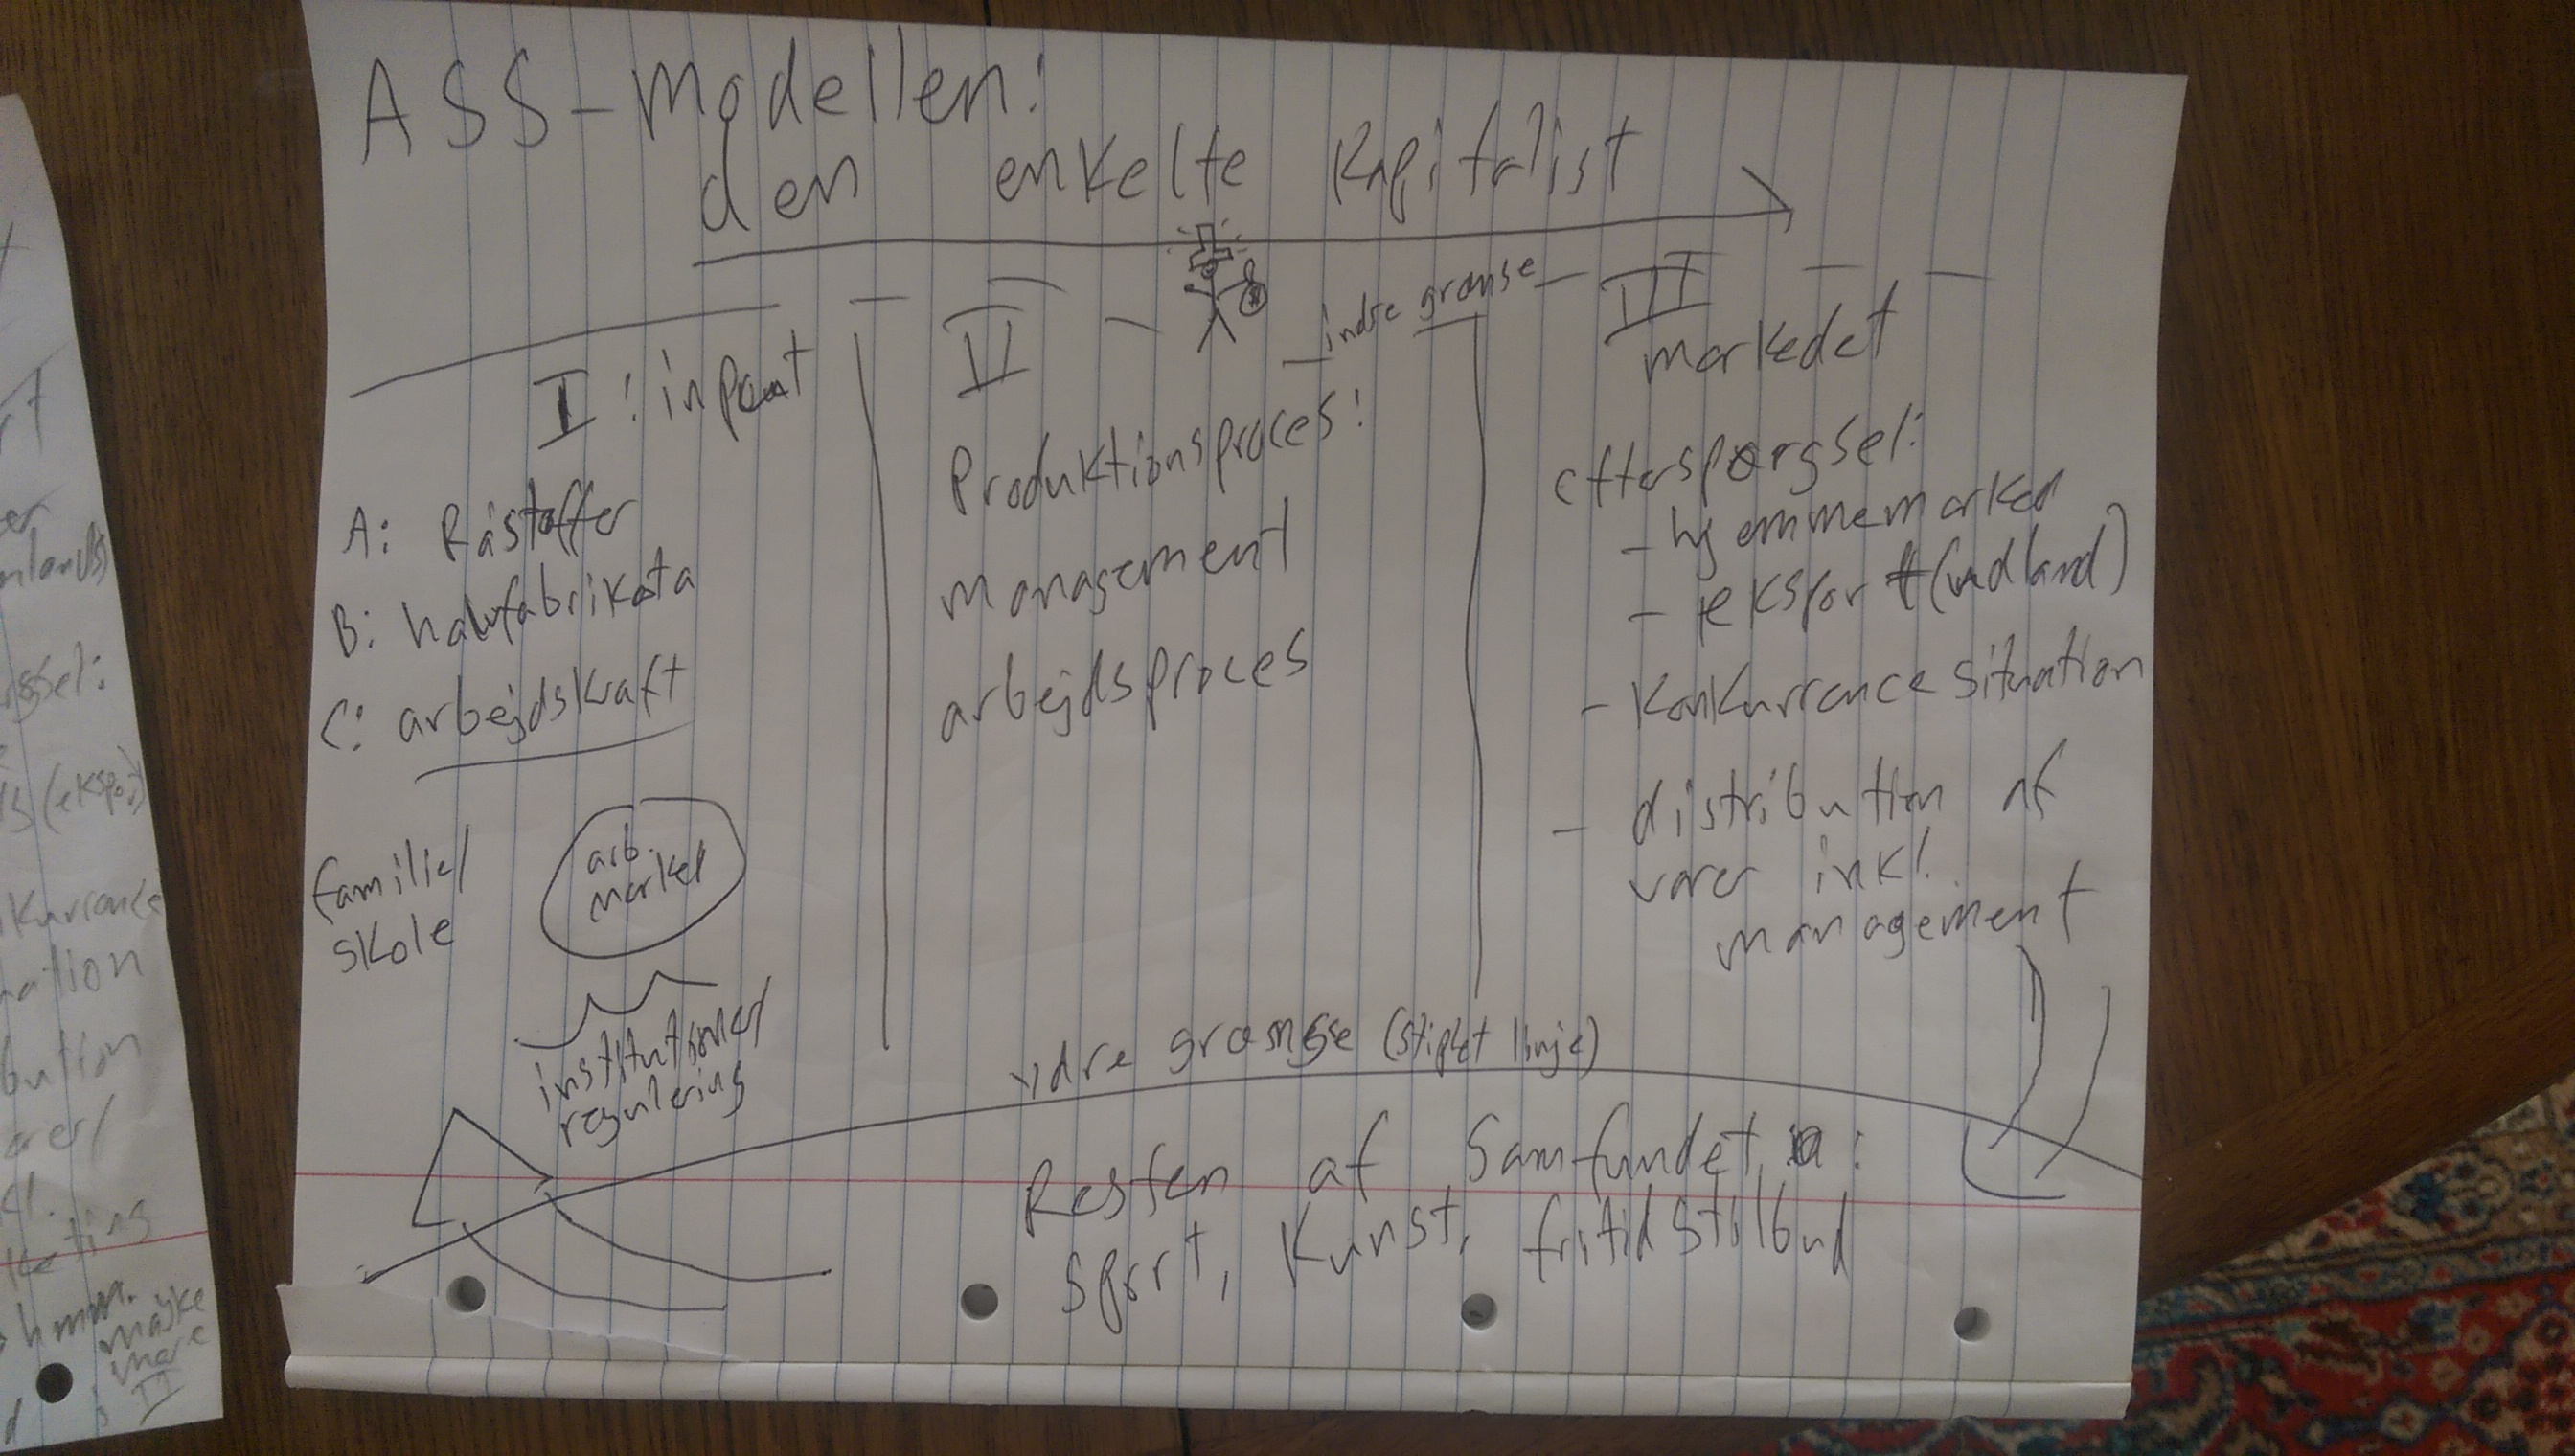
\includegraphics[width=\textwidth]{fig/ASS-model.jpg}
	\label{fig_ASSmodel}
\end{centering}
\end{figure}
%

\emph{I første fase} (I) af kapitalakkumulationen er samlingen af de nødvendige input i produktionsprocessesen. Dette inkluderer råvarer, halvfabrikata og arbejdskraft, hvoraf det sidste nævnes som den mest problematiske af de tre:  
%
\begin{quote} \small %\raggedright %(bloktekst on/off)
Labor supply, the most problematical of the three, involves both structure of the labor market, determining the immediate supply of labor, and the social institutions (family, schools, etc) that reproduce the labor force generationally\sourceatright{\parencite[24]{Gordon1982}} \label{aksocstruk}
\end{quote}
%
Efterspørgslen på arbejdskraft indeholder både arbejdsmarkedet, hvor den nødvendige arbejdskraft med de efterspurgte kompetencer købes på det påkrævne tidspunkt. Det indeholder dog også det langt større felt af sociale institutioner, der sørger for arbejdskraftens sammensætning og kompetenceniveau mere bredt forstået. Det vender jeg tilbage til.

% kunne godt referere til Fligstein her måske

\emph{Anden fase} (II) af kapitalakkumulationen foregår indenfor firmaet selv. Det indeholder organisering af selve arbejdsprocessen og management-strukturen i firmaet. Den fase kan siges ikke at have så meget med miljøet at gøre som med firmaets interne organisering. GER påpeger at det, der her tilsigtes, er de normer og erfaringer for organisering og management, som firmaerne trækker på, og som derfor er en del af den sociale struktur, det enkelte firma trækker på i dets akkumulationsproces. Denne organisering af arbejdet og ledelsen af arbejdet er central for eksempelvis fagforeningernes betingelser for at organisering. Det har også - lidt mere diffust men ikke mindre vigtigt - vidtrækkende konsekvenser for de livserfaringer, det enkelte menneske gør sig, og dermed hvordan det fortolker verden omkring sig. (REFERENCEMÅSKE? Gruskys kulturelle funktionalisme kunne nævnes her \#todo). 

\emph{Den tredje fase} (III) er salgsprocessen, hvori vareefterspørgsel,  samt status for konkurrencetilstande på det specifikke marked, et givent firma producerer til. Det kunne eksempelvis en være monopollignende tilstand, hvilket muliggør en bestemt virksomhedsstruktur. 

Det er særligt første og anden fase, der har min interesse, da mit fokus er arbejdsmarkedet og dets relation til klassestrukturen. Tredje fase har dog en meget vigtig mekanisme i relation til arbejdsmarkedets segmentering, ifølge GER, som bør fremhæves, og som leder over i GERs teori om det tredelte arbejdsmarked og forklaringen på denne.

Konkurrencetilstanden på markedet har betydning for arbejdsmarkedet generelt, ikke bare af den åbenlyse grund, at det skaber den økonomiske virkelighed for de virksomheder, lønmodtagerne er ansat i. Konkurrencetilstanden på markedet er også en af de væsentligste forudsætninger i GERs segmenteringsteori om et todelt arbejdsmarked. De viser hvordan man I USA fra 30'erne og frem udviklede store firmaer, med stabile profitrater og undertiden monopollignende markedsandele, såvel på hjemmemarkedet som internationalt. Disse firmaers størrelse og stabilitet gav mulighed for \emph{interne arbejdsmarkeder}, hvorigennem kompetencer kan udvikles internt, karrieremuligheder sikrer loyalitet, og andre fordele forbundet med hvad GER kalder \emph{bureaukratisk kontrol}. Dermed menes der management systemer, der strukturerer og sikrer størst mulig samarbejdsvillighed og produktivitet fra arbejderne i arbejdsprocessesen, baseret på nedskrevne love og regler. Det er en af årsagerne til fremkomsten af interne arbejdsmarkeder i store firmaer, der af GER karakteriseres som \emph{kernesegmentet/det primære segment} \parencite[187]{Gordon1982}. Det svært for firmaer fungerende på usikre markeder med lav profitrate at skabe disse strukturer, dette opstår derfor de mest stabile og moderne kapitalisske firmaer, de tenderende-til-monopolitiske, kunne man kan kalde dem.

På denne måde kan vi se at de fem dynamiske tendenser nævnt på \pref{kapitalakkumulation} hænger sammen med den akkumulations sociale struktur, hvorigennem disse lovmæssigheder i en marxistisk optik fungerer. Den femte tendens, arbejdernes modstand, er central for at forstå logikken i segmenteringens opståen, ifølge GER. Det er arbejdernes modtræk, og ikke mindst arbejdsgivernes modtræk til disse modtræk, så at sige. 
Fagforeninger spiller derfor en væsentlig rolle. Det er GERs argument, at fagforeningers styrkeposition fra 30'erne og frem, også i USA, banede vejen for et klassekompromis, hvor arbejdsgiverne blev tvunget til at give indrømmelser omkring stabile ansættelser, reallønstigninger og sikre arbejdsforhold. En række krav blev imødekommet, og arbejdsgiverne var til en vis grad var klar over nødvendigheden af dette. Den tidligere sociale akkumuleringsstruktur, som GER analyserer klassificerer som \emph{homogeniseringsperioden} fra 1870 til slutningen af Anden Verdenskrig, mente man, gavnede radikale elementer i arbejderbevægelsen, da denne skabte homogenitet i klassestrukturen blandt arbejderklassens forskellige fraktioner. Derfor var visse indrømmelser at foretrække. Der var desuden nok at gøre med at tilrettelægge arbejdsprocessen til ny teknologi og nye måder at styre, uddanne og inddele arbejdsstyrken på. Her kunne fagforeninger også bruges som nødvendige samarbejdspartnere \parencite[186f]{Gordon1982}. Denne overgivelse af magt over arbejdsprocessen, som fagforeninger gav - eller blev tvunget til - attribuerer GER til tre hovedårsager, nemlig muligheden for reallønstigninger og sikringer af arbejdstagerrettigheder. Det  muliggjordes af det økonomiske boom efter 2. Verdenskrig. De to andre faktorer var udrensning af radikale elementer i fagforeningerne i McCarthy-æraen, samt den manglende evne til at forstå hvad denne overgivelse af magt til arbejdsgiverne i arbejdsprocessen betød for lønmodtagernes styrkeposition. Dette danner basis for en primærøkonomi og en perifær økonomi, der skal gennemgås nu.

%%%%%%%%%%%%%%%%%%%%%%%%%%%%%%%%%%%%%%%%%%%%%%
\section{De to primære segmenter og det sekundære segment \label{AST_primuafprimundersekundaer}}
%%%%%%%%%%%%%%%%%%%%%%%%%%%%%%%%%%%%%%%%%%%%%%


Logikken i det nye system, der derved blev udviklet, kan opsummeres på følgende vis: Jobs blev findelt i specifikke jobfunktioner, ofte indenfor trin i en karriertrappe. Ny teknologi påvirkede ikke kun hastigheden og arbejdskvaliteten, men blev også benyttet med det bredere formål at akkomodere managementpolitik, reguleringen af arbejdet og arbejderne som sådan. Ansættelser, forfremmelser og afskedigelser blev systematiseret og bureaukratiseret. Forhandlinger mellem arbejdergiver-fagforeninger blev i højere grad et spørgsmål om løn og frynsegoder, mens arbejdsforholdene og arbejdspladsens indretning blev til managementpolitik, udviklet af ingeniører og forløberne til HR-konsulenter. Det betyder at arbejdsmanagement skiftede karakter fra en intervention fra ledere eller mellemledere og deres direkte autoritet, til et spørgsmål om regulativer og procedurer \parencite[189]{Gordon1982}%
%
\footnote{Udviklingen af bureaukratisk autoritet er en tendens Max Weber beskriver så tidligt som i 20'erne. Jeg anskuer det sådan, at GER viser hvorledes denne autoritetsform rodfæster sig i den samfundsmæssige produktion i årtierne efter, og at dens konkrete udformning og formål - udover at have sin egen indre logik, jvf. “rationalitetens jernbur” - sker på basis af magtkampe mellem klasserne. (FIND HENVISNING WEBER).}%
%
. 

Det betyder dog ikke, at alle arbejdstagere i den primære økonomi har samme forhold. GERs såkaldt todelte arbejdsmarkedsteori er mere en teori om et \emph{tredelt} arbejdsmarked. Deres fokus på \emph{firmaer} som central økononomisk enhed, samt den i forvejen etablerede forskning om center-periferien i amerikansk økonomi, får dem til at tale om det primære og sekundære segment, fordi det er sådan, det findes på firma-niveau. Hvis man kigger på beskæftigelsesforhold, viser GERs analyse imidlertidig en opdeling af arbejdet i primærfirmaer i to segmenter: Det \emph{“primære uafhængige”} segment og det “\emph{primære underordnede}” segment. Disse segmenter fungerer i store firmaer med de tidligere nævnte karakteristikker, og begge segmenter har, relativt til det sekundære segment, højere lønninger, bedre jobsikkerhed og mulighed for karriereveje \parencite[202]{Gordon1982} \label{GERs tre segmenter}. Det er denne virksomhedsstruktur, der danner basis for det primære segment af arbejdstagere.

Det \emph{sekundære/perifære} segment består af job i små og mellemstore virksomheder, ofte ejet af et enkelt individ eller en familie, i begrænsede markedspositioner, tit med usikker eller stærkt variende efterspørgsmål. Profitten er typisk lavere end i kerneøkonomien%
%
\footnote{betegnelserne kerneøkonomi og den perifære økonomi er stammer fra den amerikanske økonom Robert Averitt, der i 60'erne benyttede denne betegnelse til at forstå den amerikanske økonomi, dog ikke ud fra det klasseperspektiv GER benytter i deres segmenteringsteori. Det her står vist også et andet sted \#todo}%
%
, og økonomiske kriser resulterer ofte i konkurs eller alvorlige finansielle problemer. Teknologi og marketing er sjældent up to date med firmaer i kerneøkonomien \parencite[7]{Averitt1968}. Det sekundære arbejdsmarked har som følge deraf lavere lønninger, større risiko for arbejdsløshed, mange midlertidige  stillinger og andre dårlige ansættelsesforhold \parencite[70f]{Doeringer1971}.

GER peger på at firmaer i den perifære økonomi tjener et formål, og der er grunde til at de ikke overtages af kernefirmaerne: Det er usikre markeder med svingende, ofte lavt, afkast. Det giver kernefirmaer mulighed for outsourcing af bestemte opgaver, der er billigere end indenfor de restriktioner, det primære beskæftigelsessegment muliggør. Særligt i forbindelse med varierende efterspørgsel: Det giver en fleksibilitet i at kunne hyre arbejdere fra det sekundære segment indirekte, gennem et sekundært firma, når efterspørgslen på et primærfirmas varer er høj, uden at være bundet op på forpligtigelser når efterspørgslen er lav \parencite[191]{Gordon1982}. 

Det primære uafhængige segment \label{GER kontrol og intern arb marked} indeholder de højere uddannede lønmodtagere indenfor professionerne, management og teknisk arbejde. De oplever et højere økonomisk afkast ved deres uddannelse%
% 
\footnote{GER skriver at de opnår “\emph{a higher return to schooling and experience}” \parencite[202]{Gordon1982}, hvilket jeg tolker som \emph{relativt} til det underordnede segment, det vil sige at de økonomisk får mere ud af x antal års uddannelse eller erfaring end en person beskæftiget i det underordnede segment.}%
%
, og der er sjældent en direkte supervision af og autoritetsudøvelse over udførslen af deres arbejde. De er desuden tilbøjelige til at internalisere firmaets formål. 
Historisk udspringer dette, ifølge GER, af proletariseringen og de deraf følgende konsekvenser af nogle traditionelle klasser i forbindelse med kapitalismens tidligere akkummulationsstruktur, i GERs jargon kaldet \emph{homogeniseringsperioden}.  Dette skete indenfor eksempelvis håndværkerlaug, samt andre med højtudviklede faglige ekspertiser. Ekspertise på de niveauer var i midlertidigt en nødvendighed, og en omkalfatring af disse traditionelle klasser ledte til fremkomsten af positioner i den primære økonomi, hvoraf formel uddannelse med tæt tilknytning til “arbejdsmarkedets behov”, altså arbejdsgivernes behov, fandt sted. Det skete  ifølge GER ikke uden magtkampe mellem klasserne, så GER pointerer at disse erhvervsgruppers nuværende position også er et resultat af de modtræk, erhvervsgrupperne benyttede sig af, for at sikre sig autonomi og andre goder, eksempelvis ved oprettelsen af hvad GER kalder “professionelle associationer”, man kunne forestille sig at DJØF og IDA kunne eksempler i en dansk kontekst. Resultatet af denne torvtrækning med arbejdsgiverne, til en vis grad vellykket, betød følgelig skarpere segmentering ifht. det primære underordnede segment \parencite[202f]{Gordon1982}.

Dette kan ogsåDet \emph{sekundære/perifære} segment består af job i små og mellemstore virksomheder, ofte ejet af et enkelt individ eller en familie, i begrænsede markedspositioner, tit med usikker eller stærkt variende efterspørgsmål. Profitten er typisk lavere end i kerneøkonomien%
%
\footnote{betegnelserne kerneøkonomi og den perifære økonomi er stammer fra den amerikanske økonom Robert Averitt, der i 60'erne benyttede denne betegnelse til at forstå den amerikanske økonomi, dog ikke ud fra det klasseperspektiv GER benytter i deres segmenteringsteori. Det her står vist også et andet sted \#todo}%
%
, og økonomiske kriser resulterer ofte i konkurs eller alvorlige finansielle problemer. Teknologi og marketing er sjældent up to date med firmaer i kerneøkonomien \parencite[7]{Averitt1968}. Det sekundære arbejdsmarked har som følge deraf lavere lønninger, større risiko for arbejdsløshed, mange midlertidige  stillinger og andre dårlige ansættelsesforhold \parencite[70f]{Doeringer1971}.

GER peger på at firmaer i den perifære økonomi tjener et formål, og der er grunde til at de ikke overtages af kernefirmaerne: Det er usikre markeder med svingende, ofte lavt, afkast. Det giver kernefirmaer mulighed for outsourcing af bestemte opgaver, der er billigere end indenfor de restriktioner, det primære beskæftigelsessegment muliggør. Særligt i forbindelse med varierende efterspørgsel: Det giver en fleksibilitet i at kunne hyre arbejdere fra det sekundære segment indirekte, gennem et sekundært firma, når efterspørgslen på et primærfirmas varer er høj, uden at være bundet op på forpligtigelser når efterspørgslen er lav \parencite[191]{Gordon1982}. 

Det primære uafhængige segment \label{GER kontrol og intern arb marked} indeholder de højere uddannede lønmodtagere indenfor professionerne, management og teknisk arbejde. De oplever et højere økonomisk afkast ved deres uddannelse%
% 
\footnote{GER skriver at de opnår “\emph{a higher return to schooling and experience}” \parencite[202]{Gordon1982}, hvilket jeg tolker som \emph{relativt} til det underordnede segment, det vil sige at de økonomisk får mere ud af x antal års uddannelse eller erfaring end en person beskæftiget i det underordnede segment.}%
%
, og der er sjældent en direkte supervision af og autoritetsudøvelse over udførslen af deres arbejde. De er desuden tilbøjelige til at internalisere firmaets formål. 
Historisk udspringer dette, ifølge GER, af proletariseringen og de deraf følgende konsekvenser af nogle traditionelle klasser i forbindelse med kapitalismens tidligere akkummulationsstruktur, i GERs jargon kaldet \emph{homogeniseringsperioden}.  Dette skete indenfor eksempelvis håndværkerlaug, samt andre med højtudviklede faglige ekspertiser. Ekspertise på de niveauer var i midlertidigt en nødvendighed, og en omkalfatring af disse traditionelle klasser ledte til fremkomsten af positioner i den primære økonomi, hvoraf formel uddannelse med tæt tilknytning til “arbejdsmarkedets behov”, altså arbejdsgivernes behov, fandt sted. Det skete naturligvis ikke uden klassekamp, så GER pointerer at disse erhvervsgruppers nuværende position også er et resultat af de modtræk, erhvervsgrupperne benyttede sig af, for at sikre sig autonomi og andre goder, eksempelvis ved oprettelsen af hvad GER kalder “professionelle associationer”, man kunne forestille sig at DJØF og IDA kunne eksempler i en dansk kontekst. Resultatet af denne torvtrækning med arbejdsgiverne, til en vis grad vellykket, betød følgelig skarpere segmentering ifht. det primære underordnede segment \parencite[202f]{Gordon1982}.
Dette kan også tolkes som GERs bud på hvad Eric Olin Wright kalder “the problem of the middle classes” i marxismen, altså hvilken historisk rolle og nuværende position, man skal forstå middelklasserne i, i en marxistisk optik. Mere om det i afsnit (??? \#todo).

Det “\emph{primære underlagte}” segment har ikke nødvendigvis udsigt til betydningsfulde forfremmelser, men er i stedet motiveret af stabil jobsituation og lønforhøjelser gennem anciennitet. Deres arbejdsprocess er superviseret og indeholder meget repetitivt, rutinepræget arbejde, med specifikke regler for dets udførsel og direkte autoritetsudøvelse i forbindelse med overholdelsen af disse. Der er ikke kun tale manuelt arbejde af den traditionelle arbejderklasse-forestilling, men også ikke-manuelt arbejde indenfor “\emph{white-collar}”jobs befinder sig i det primære underordnede segment (du må ku finde på en bedre beskrivelse \#todo) .  Disse er i langt højere grad organiseret sig gennem fagforeninger, da loyalitet til arbejdsgiverne ligger fjernere for beskæftigede i dette segment end i det primære uafhængige segment. \parencite[28f]{Drago1995} og \parencite[203]{Gordon1982}. (hvordan kan jeg få de her stå i samme parentes? \#todo). tolkes som GERs bud på hvad Eric Olin Wright kalder “the problem of the middle classes” i marxistisk klasseteori: Hvilken historisk rolle og nuværende position kan man forstå fremkomsten af en lang række klassefraktioner, der ikke så let kan karakteriseres som arbejderklasse. Mere om det i afsnit (??? \#todo).

Det “\emph{primære underlagte}” segment har ikke nødvendigvis udsigt til betydningsfulde forfremmelser, men er i stedet motiveret af stabil jobsituation og lønforhøjelser gennem anciennitet. Deres arbejdsprocess er superviseret og indeholder meget repetitivt, rutinepræget arbejde, med specifikke regler for dets udførsel og direkte autoritetsudøvelse i forbindelse med overholdelsen af disse. Der er ikke kun tale manuelt arbejde af den traditionelle arbejderklasse-forestilling, men også ikke-manuelt arbejde indenfor “\emph{white-collar}”jobs befinder sig i det primære underordnede segment (du må ku finde på en bedre beskrivelse \#todo) .  Disse er i langt højere grad organiseret sig gennem fagforeninger, da loyalitet til arbejdsgiverne ligger fjernere for beskæftigede i dette segment end i det primære uafhængige segment. \parencite[28f]{Drago1995} og \parencite[203]{Gordon1982}. (hvordan kan jeg få de her stå i samme parentes? \#todo).

GERs historiske redegørelse for klasseudviklingen i USA er, naturligvis, netop dette: en redegørelse for klasseudviklingen \emph{i USA}. Det betyder at en lang række af de sociale forhold, der gør sig gældende, ikke kan overføres til andre lande. Sammensætningen og betydningen af hvilke sociale strata, der findes, hvordan middelklassepositionerne er udformet, samt hvilke politiske alliancer, der findes. Det er centralt for udformingen af et samfund, som de siger, og fortsætter: “\emph{an emphasis on human agency rather than abstract laws in historical change, (...) the importance of historical contingency in shaping the responses of different groups to capitalist development, (...) and the diverse spatial and temporal paths of capitalist development.}” \parencite[21]{Gordon1982}. 

Det er derfor tankegangen og forståelsen af, hvorledes arbejdsmarkedet fungerer i klassestrukturen, der er brugbar i min afhandling. Denne vil jeg benytte i min egen analyse. Først vil jeg kombinere den med indsigt fra Thomas Bojes udkast til en segmenteringsanalyse af det danske arbejdsmarked, specifikt hvor Boje peger på forskellen mellem in-market og pre-market segmentering.

Boje skelner mellem to former for segmentering: \emph{premarket} segmentering og \emph{inmarket} segmentering. Det er ganske simpelt forskellen på den stratifikation, der foregår på arbejdsmarkedet, og den, der finder sted før arbejdsmarkedet \parencite[46]{Boje1985}. At skelne disse fra hinanden i praksis er ikke nemt. Boje opstiller følgende model for forskellen mellem premarket og inmarket segmentering:
%
   \begin{figure}[H]
   \begin{centering}
   	\caption{Premarket og inmarket segmentering}
   	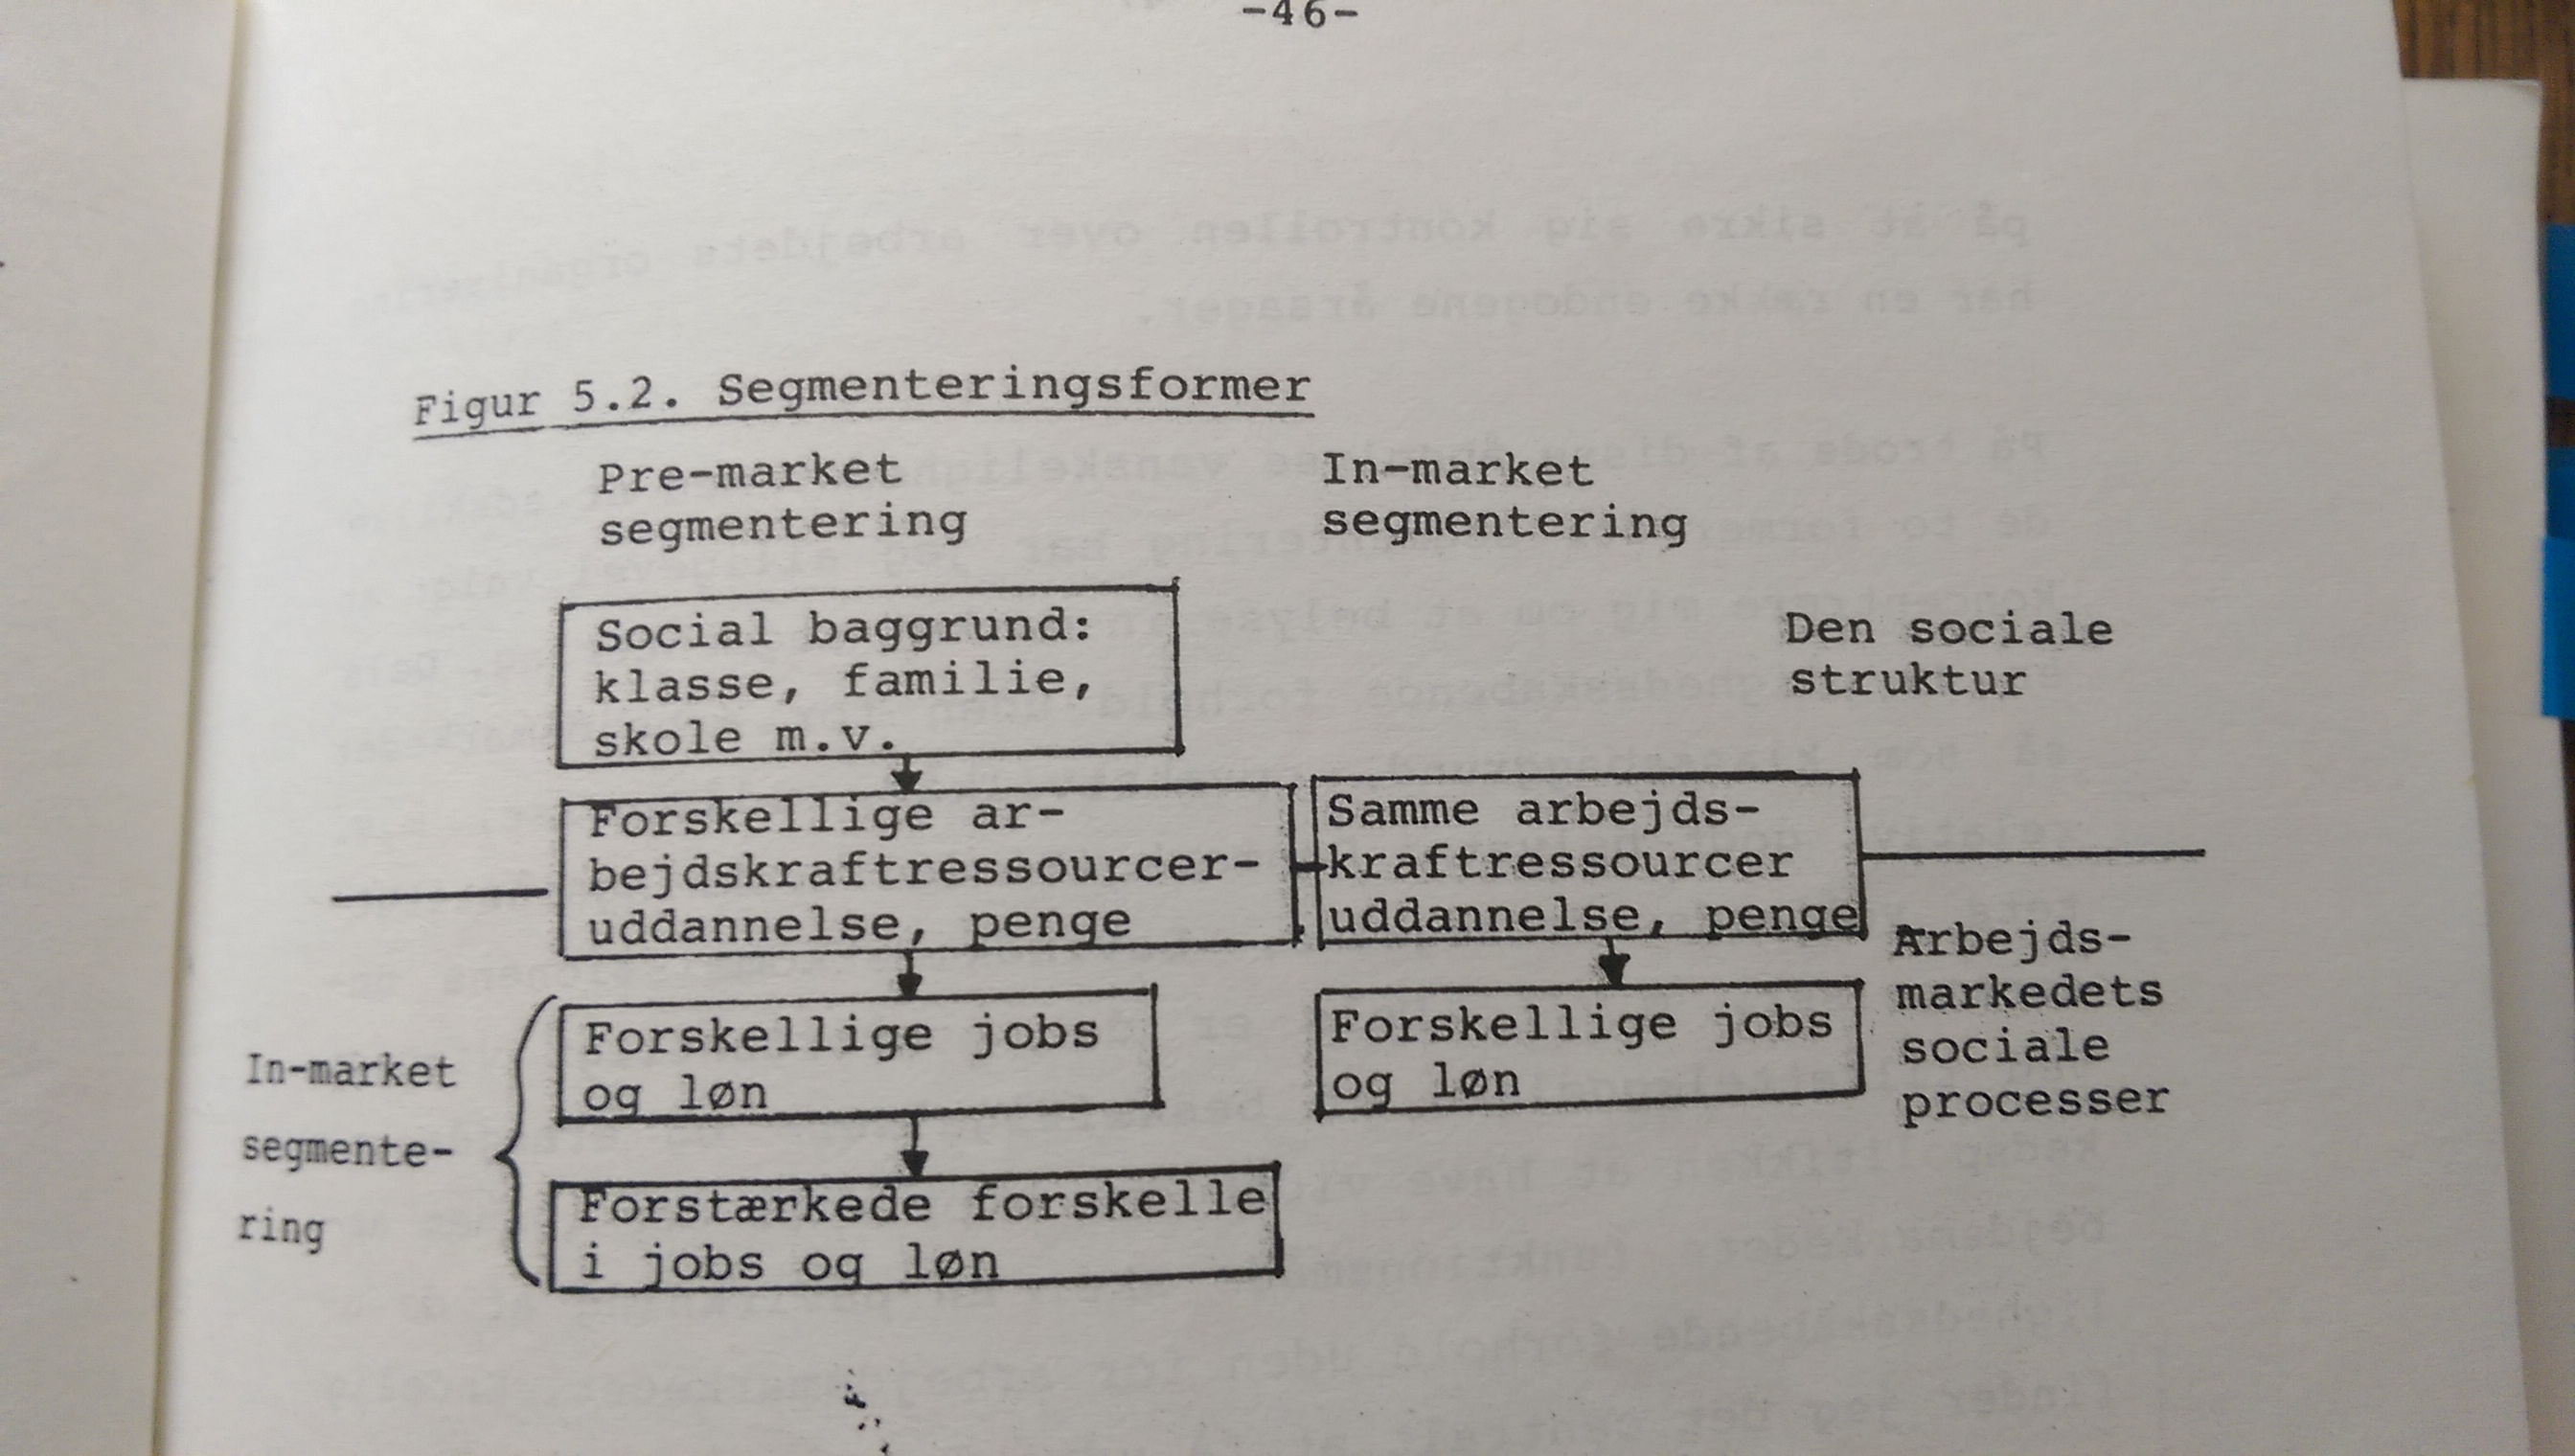
\includegraphics[width=\textwidth]{fig/Boje_premarket_inmarket.jpg}
   	\label{fig_premarketinmarket}
   \end{centering}
   \end{figure}   
%

\emph{Premarket segmentering} ligger tæt op af hvad man kunne kalde den almene sociale stratifikation i samfundet, omend fokus er rettet på de stratifikationsformer, der bevirker at lønarbejdere stilles forskelligt ved indtræden på arbejdsmarkedet. 
Eksempelvis forskelle i kvalitet af uddannelsesinstitutionerne, familiens kulturelle og økonomiske ressourcer, samt  sociale netværk i forbindelse med skolekammerater og familiekontakt, der giver forskellige ressourcer ved indtrædelse på arbejdsmarkedet. 

\emph{Inmarket segmentering} omhandler de mekanismer, der gør sig gældende på arbejdsmarkedet. Som Boje siger, er det det, som GER bruger mest i deres forklaringsmodel \parencite[46]{Boje1985}.  (vend tilbage til det her, vurder hvilke eksempler der skal med. fx race, køn \#todo).

Det kan være svært at lave en præcis grænse mellem disse to typer segmenter. I en dansk kontekst konkluderer Andrade, i en registerdata-baseret undersøgelse af nabolagseffekter på indkomstforskelle i perioden 1986-1988 og 2006-2008: “\emph{Although changes in the labour market appear to be the primary factor in the explanation of the reproduction of poor and wealthy neighborhoods, geographical movements can be viewed as a spill-over-effect in which individuals who no longer fit the socioeconomic profile of the neighborhood moves out of the the neighborhoods. These selection processses of geographical mobility in and out of neighborhoods have an active role in changing the neighborhood enviroment.}” \parencite[134]{Andrade2014}. Det vil sige, at selv det (kultur)geografiske landskab er påvirket af arbejdsmarkedets sammensætning - arbejdsmarkedet påvirker premarket segmenteringen, her forstået som geografiske fordelinger af forskellige arbejdstagere i landet. Denne socioøkonomiske fordeling, der hører ind under premarket segmentering, virker tilbage pp mulighederne på arbejdsmarkedet, altså inmarket segmenteringen. Hvad, som man siger, kom først: Hønen eller ægget? Hvor svaret naturligvis er, at det er det forkerte spørgsmål at stille i den sammenhæng, fordi der ikke er en \emph{sui genesis} kausalitet på spil. Det gælder denne kulturgeografiske - klassemæssige sammenhæng, såvel som den gælder opdelingen mellem inmarket - og premarket segmentering. 

Derfor kan det naturligvis \emph{analytisk} give mening at lave et klart skel mellem sociale processer, der foregår direkte på arbejdsmarkedet, og de processer, der er en del af hele klassestrukturen. Det er inkorporeret i følgende udvikling af ASS-modellen, nu kaldet B-ASS (for Boje): 
%
\begin{figure}[H]
\begin{centering}
	\caption{B-ASS modellen}
	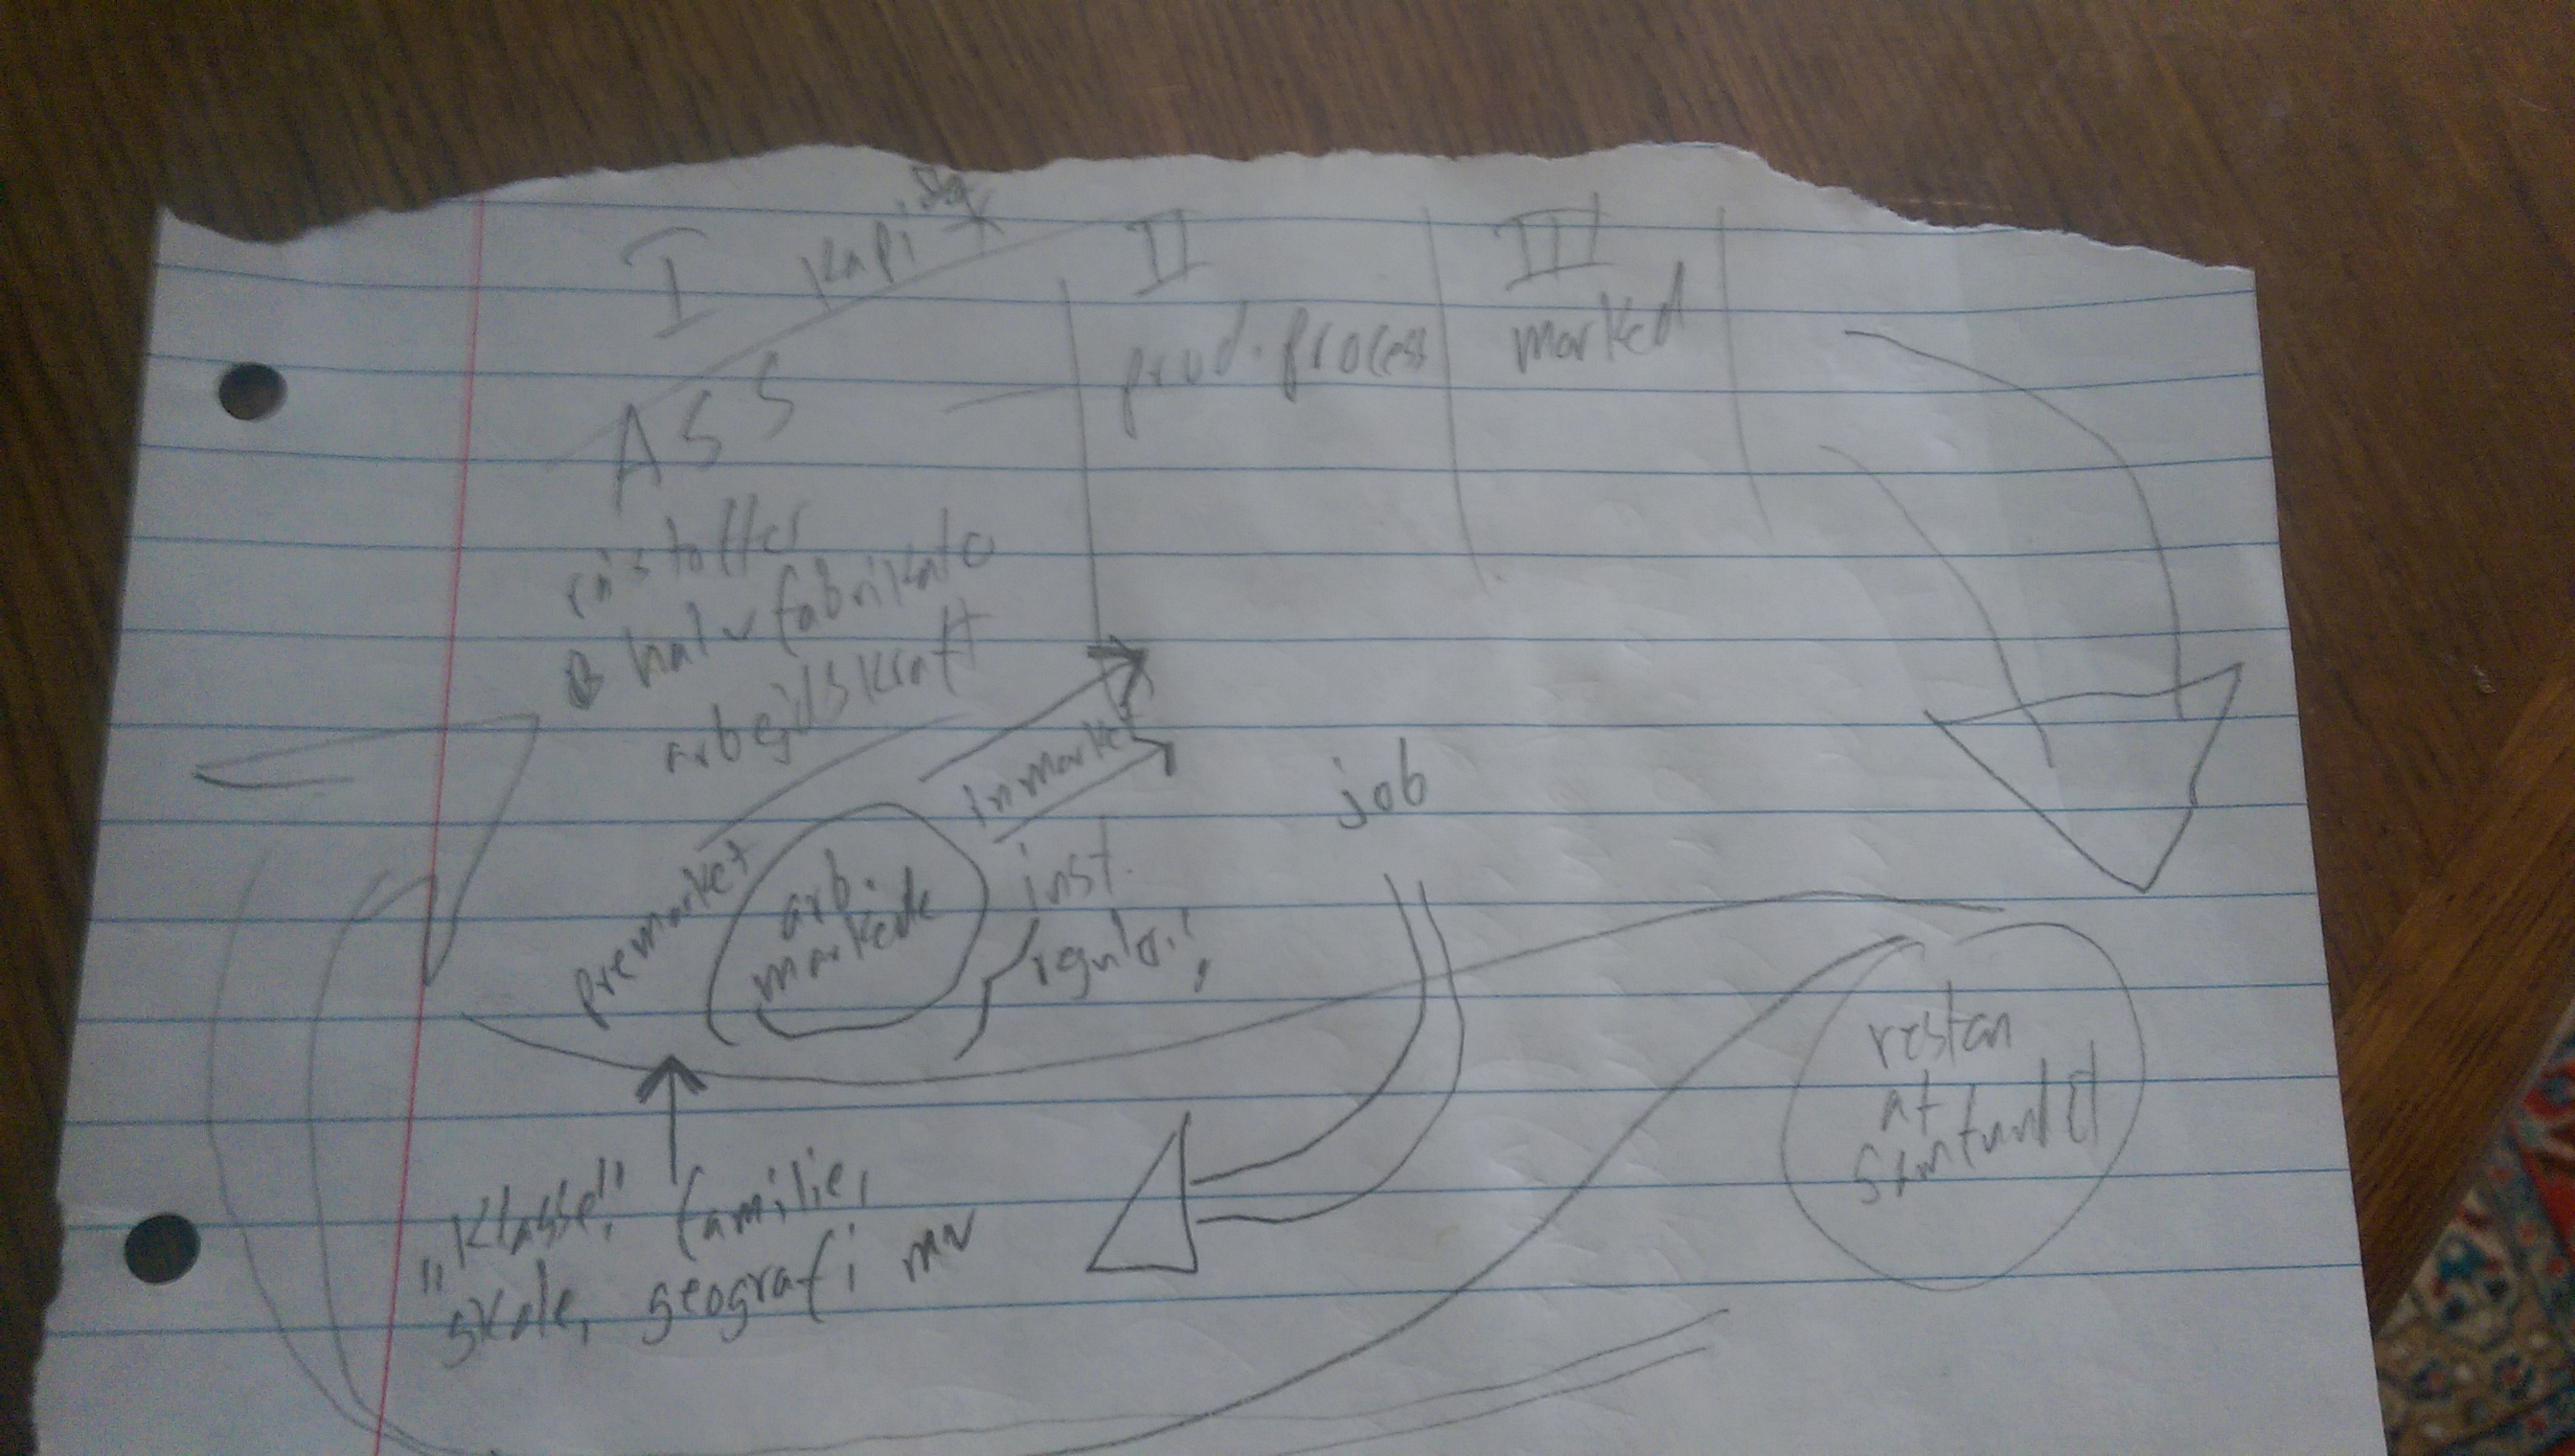
\includegraphics[width=\textwidth]{fig/B-ASS-model.jpg}
	\label{fig_B-ASSmodel}
\end{centering}
\end{figure}
%

manger ordentlig gennemgang af B-ASS modellen \#todo.


%%%%%%%%%%%%%%%%%%%%%%%%%%%%%%%%%%%%%%%%%%%%%%
\chapter{Empiriske resultater og metodologiske udfordringer  \label{teori_AST_metodeogempiri}}
%%%%%%%%%%%%%%%%%%%%%%%%%%%%%%%%%%%%%%%%%%%%%%


Skriv bedre indledning \#todo

Derudover har GERs teori samt empiri nogle problemer, der skal adresseres. Først de empiriske udfordringer samt bud på kortlægninger af segmenter, jeg har set på.

Det er en generel udfordring i segmenteringsteori, at der er meget lidt enighed om hvad der præcist karakteriserer et segment, hvordan segmenter er adskilt fra hinanden, og følgelig hvordan man empirisk observerer segmenter \parencite[71]{Leontaridi1998}, \parencite[1231]{Cain1976}. Følgelig er de indikatorerer og variable, der benyttes til at observere segmenter, vidt forskellige. Jeg vil her beskrive tre strategier, som jeg ser i litteraturen. Disse tre strategier benytter sig af forskellige variable, samt forskellige statistiske teknikker. 

Gordon, Edwards og Reich er overraskende vage i deres empiriske definition af hvad der udgør et segment, og hvordan det bør måles.
De benytter selv data på branche-niveau, men siger at brancher  indeholder både kerne- og perifæri firmaer. De mener med andre ord at data på firmaniveau er ideelt, men har ikke sådanne data til rådighed selv \parencite[193]{Gordon1982}. De indikatorer, de benytter sig af, er primært mål for økonomisk formåen på brancheniveau, hvori beviset for den 3-delte segmentering, de a priori har inddelt brancherne i, handler om den relative forskel mellem segmenterne på en række indikatorer, og særligt en stigende relativ forskel over tid. 
Det er indikatorer såsom værdi tilført per arbejder, lønforskelle per arbejder, andelen af manuelt arbejdende i forhold til ikke-manuelt arbejdende i firmaet, samt faglig organisering i branchen. Alle disse sættes op relativt mellem GERs på forhånd inddelte 3-delte segmentopldeing \parencite[193]{Gordon1982}. 

Derudover kommer de med to interessante betragtninger om ting de \emph{ikke} har kunne måle: Udover at de helst ville have data på firma-niveauer, siger de også at indenfor firmaer i den primære økonomi, findes der sekundære og primære jobtyper. Derfor ville data på beskæftigelsesniveau fremfor firma- og branche være interessant, mener de \parencite[193]{Gordon1982}. 

Det andet de siger er de løb ind i problemer, da de skulle opdele ikke-manufaktur brancher i kerne-perifæri, da denne distinktion ikke let lader sig overføre udenfor den direkte materielle produktion af goder. Derfor er deres undersøgelse \emph{en undersøgelse af en tre-delt segmenteringsproces indenfor manufakturen i USA} \parencite[199]{Gordon1982}, mens segmentstrukturen andre steder i arbejdsmarkedet kan være anderledes indrettet, også i USA på det tidspunkt.

Man kan sammenfatte og sige at denne metode inddeler brancher efter en teoretisk styret logik baseret på et tre-delt arbejdsmarked, og benytter økonomiske nøgletal på brancheniveau som variable. Nøgletallene er antageligt populationsbaserede, fremfor survey-baseret (bliv sikker på det her senere \#todo) Herefter benyttes forskellene i nøgletallene mellem de tre teoretisk inddelte segmenter til at teste hypoteser om forskelle på segmenterne. De benyttede variable har et fokus på produktion og fagforeningsorganisering til at lave denne tredeling.  

Den anden strategi er benyttet i en australsk undersøgelse fra 1995, hvor Robert Drago (1995) finder at den tredelte segmentstruktur beskrevet af GER passer med det australske arbejdsmarked. Her benyttes survey-data på firma-niveau, og metoden er en  konfirmatorisk klusteranalyse. Det vil sige antallet af klustre er bestemt ex ante til GERs tre segmenter. At observationsenheden er firmaer, giver nogle problemer, bemærker Drago selv, da firmaer godt kan indeholde job fra forskellige segmenter, men denne undersøgelse gør det til enten-eller. Variablene er andelen af manuelt arbejdende i forhold til ikke-manuelt arbejdende i firmaet, andelen af ansatte med jobancienittet på mindst 10 år, andelen af deltidsansatte, andelen af kvindelige ansatte, lønningsniveauer, andelen af supervisorer der er steget i graderne internt i firmaet og deslige. Drago finder at de tre klustres karakteristikker passer overordentligt godt med den tredelte segmentstruktur i GERs segmenteringsteori \parencite[59]{Drago1995}. 

Man kan sige sammenfatte og sige at her er den empiriske metode ganske avanceret, og baseret en survey hvor observationsenheden er firmaer, som anbefalet af GER selv. Segmentinddelingen af firmaerne er ikke lavet af forskerne selv, men af en konfirmatorisk klusteranalyse, der baserer sine grupperinger på minimal varians af variable indenfor det på forhånd fastsatte antal klustre. Selve variablene er mindre fokuseret på økonomisk formåen i segmenterne og mere fokuseret på arbejdsmiljø. 

Gittleman og Howell (1995) benytter ligeles klusteranalyse deres undersøgelse af segmenter, men ud fra et andet udgangspunkt. De opsummerer segmenteringsteoretikernes empiriske forsøg på følgende vis: “\emph{the most common approach in empirical studies of segmentation, particularly when the unit of analysis is occupations, has been to begin with the researcher's judgment about how many and what kind of rules to empirically implement the scheme, again based on the researcher's judgment. (...) the arbitrariness of this approach has been sharply critized.}” \parencite[422]{Gittleman1995}. Derfor benytter de i stedet en eksplorativ klusteranalyse, hvor antallet af segmenter ikke er defineret på forhånd. De benytter Wards hierarkisk-agglomerative klusterteknik. Det betyder at klustre merges sammen på stadig højere niveauer, sådan at to klustre, der merges på 2. niveau af klusterproceduren, hver især godt kan være sammenlægninger af tidligere klustre på 1. niveau, og så fremdeles, indtil visse varians-kriterier er opfyldt \parencite[425]{Gittleman1995}.
Man kunne måske forledes til at tro at de mener en udelukkende mekanisk inddeling er at foretrække, det er dog for simpelt. De når frem til 6 klustre, hvor de udelader en 7. kluster af teoretisk-praktiske grunde - de argumenterer for denne 7. gruppe er en undergruppe af et af de andre segmenter, da de sammenlagte jobtyper ikke adskiler sig væsentligt \emph{på et teoretisk niveau indenfor segmenteringsframeworket} fra den klynge, den kommer fra \parencite[424]{Gittleman1995}. Så der er mere tale om at beslutte sig for en deskriptiv statistisk teknik, hvorigennem ligheder og forskelle defineres ud fra, og et bud på en segmenteringsstruktur foreligger. Og derefter fortolke denne struktur teoretisk, finde ud af hvor den simpelthen ikke giver mening, fordi den udelukkende er teknisk fremstillet, og modificere de tekniske parametre, der ligger til grund, således at en meningsfuld model kan benyttes. Altså en abduktiv empirisk tilgang (find reference på abduktiv \#todo). Men grundlæggende 

De benyttede variable kommer fra en survey om arbejdskvalitet, og detaljerede informationer om respondernes beskæftigelse samt branche-tilhørsforhold. Gittleman og Howell benytter altså en kombination af jobs og branche for at kunne se forskel på \emph{samme} jobs indenfor \emph{forskellige} brancher, og forskellige jobs indenfor \emph{samme} branche. 
Det er vigtigt at bemærke at denne at segmentopdelingen, ligesom hos Drago, baserer sig på en række mål for kvaliteten af jobs. Det er ud fra en grundbetragning om at \emph{jobkvalitet}, og forskellene i disse, er definerende for hvad et segment er. 

Gittleman og Howell finder 6 \emph{jobkonturer}, som de kalder dem. De argumenterer for at disse jobklustre/konturer er underopdelinger af de tre segmenter beskrevet tidligere. De bemærker at en lignende undersøgelse baseret på stort set samme metode, men med et andet udvalg af survey-variable til beskrivelse af arbejdsforhold kom frem til den modsatte konklusion: at den fundne segmentering ikke passede ind i segmenteringsteorien om det tredelte arbejdsmarked \parencite[428]{Gittleman1995}. 

Ovenstående to undersøgelser, såvel som GERs rudimentære empiriske arbejde, konstruerer segmenter baseret på enshed i aflønning, jobsikkerhed, organiseringsgrad med mere.  
Andre har fremført, at eksistensen af gode og dårlige arbejdsforhold i forskelige grupper af arbejdskategorier ikke er nok. Mobiliteten mellem jobs i forskellige segmenter må være stærkt begrænsede \parencite[92]{Leontaridi1998}, \parencite[793]{DickensLang1985}%
%
\footnote{I deres artikel hvori de vurderer arbejdssegmenteringsteorierne, mener de nyklassisistiske økonomer Dickens \& Lang sågar at }%
%


%%%%%%%%%%%%%%%%%%%%%%%%%%%%%%%%%%%%%%%%%%%%%%
\section{Jobmobilitet som mål \label{teori_AST_jobmobmaal}}
%%%%%%%%%%%%%%%%%%%%%%%%%%%%%%%%%%%%%%%%%%%%%%

Det er en central hypotese i arbejdsmarkedssegmenteringensteorierne, at mobilitet mellem delmarkederne ikke finder sted, eller i det mindste finder sted i så lav grad, at det er betydningsløst. En række undersøgelserne fra 70'erne og 80'erne kom frem til tvetydige resultater: Nogle finder  stærk mobilitet mellem delmarkederne, både intra- og intergenerationelt, mens andre finder det modsatte. Graden af mobilitet er omdiskuteret, ikke mindst fordi disse undersøgelser lider af betydelige metodiske problemer \parencite[80]{BojeToft1989}. Selvom jobmobiliteten skulle være relativt høj mellem delmarkederne, anfører Boje, at det centrale spørgsmål ikke er, hvorvidt der er mobilitet eller ej, men om løndannelsen påvirkes af delmarkedernes mobilitet. Det skal forstås i kontekst af diskussionen med de nyklassististiske økonomer. I dette teoretiske perspektiv vil selv lav mobilitet mellem delmarkederne betyde, at markedsmekanismernes værdisættelsen af arbejdskraft vil allokere den humane kapital effektivt:  “\emph{If an individual can move out of the secondary sector in order to obtain returns on experience or education, the existence of a sector in which there are no returns is inconsequential}” \parencite[793]{DickensLang1985}. Det vil i mange sociologisk funderede teorier blive opfattet som stærkt reduktivt, og det er derfor essentielt for Boje, at løndannelsen (værdisættelsen) sker ud fra sociale processer i delmarkederne, hvori større eller mindre mobilitet mellem delmarkederne ikke er lig effektiv allokering ud fra markedsmekanismerne. Dickens \& Lang rejser et vigtigt kritisk spørgsmål: Hvilken betydning delmarkederne har delmarkederne egentligt, hvis mobilitet af en hvis størelse eksisterer mellem dem?  Deres affejning af betydning af delmarkeder i det hele taget, hvis mobilitet eksisterer, forekommer mig dog forhastet. Meget peger på, at traditionelle human kapital-variable som uddannelse, arbejdserfaring og alder har stor betydning for individets mobilitet. Nyere undersøgelser har især koncentreret sig om mobilitetsforskelle ud fra køn og etnicitet, hvor forskellene er substantielle \parencite[93-4]{Leontaridi1998}. % (læs dem og find henvisninger, Leontaridi s. 93-4 \#todo)




Det er en central del af GERs teori om det tredelte arbejdsmarked,

 De referede undersøgelser undersøger ikke mobiliteten mellem jobs, og de benytter mål for kvaliteten af jobs som mål for segmentinddelingen. Andre empiriske undersøgelser af segmenteringsteori vælger i stedet mobilitet mellem jobs som grundlag for inddeling.


% Som fremført på \pref{GER kontrol og intern arb marked}, mener de et internt arbejdsmarked eksisterer for det primære segment, som hindrer adgangen til disse jobs. Og indenfor dette er forskelle i arbejdsfunktioner, i form af ekspertviden og mulighed for supervisering, med til at lave yderligere en barriere, der bl.a. går på mobilitet. Det er en central del af de sociale lukningsmekanismer, der muliggør en ulige fordeling af hvad man lidt upræcist kunne kalde gode jobs. 



%%%%%%%%%%%%%%%%%%%%%%%%%%%%%%%%%%%%%%%%%%%%%%
% #Noter 
%%%%%%%%%%%%%%%%%%%%%%%%%%%%%%%%%%%%%%%%%%%%%%
% 
% Husk at ryd op i begrebsapparatet så du først begynder at definere segmenter efter klasseteorien, kritiser de tidligere segmentent teoretikeres løse brug af segmenter. 
% argument fra erik møller hansen om forskel i at se på lighed eller social mobilitet som et samfunds reason d' tetre? 

%
%
%
%
%
%
%
%
%
%
%
%
%
%
%












%!TEX root = ../report.tex

%%%%%%%%%%%%%%%%%%%%%%%%%%%%%%%%%%%%%%%%%%%%%%%%%%%%%%%%%%%
\chapter{Klasseteori som forklaringer \label{kapitel_teori_klasse}}
%%%%%%%%%%%%%%%%%%%%%%%%%%%%%%%%%%%%%%%%%%%%%%%%%%%%%%%%%%%
%klasse er et analytisk framework til at forstå segmenteringsprossesen

Klasse vil i denne afhandling benyttes til at forstå de sociale processer i segmenteringen. Samtidig vil der argumenteres for, at mobilitet mellem jobs på arbejdsmarkedet fanger et centralt aspekt af hvad klasse er, og kan bruges til at forstå \emph{arbejdets logik} i dagens Danmark. Jeg vil tage udgangspunkt i klassebegrebet, som det analytisk framework til at forstå segmenteringsprocessen  og de forskellige bud på klasser, da intet begreb i sociologien er så nært knyttet op på en forståelse af de sociale processer i arbejdslivet. 

Klassebegrebet har gennem de sidste ti år haft en genopblomstring, omend med en noget andet betoning end tidligere. %indsæt evt det det at det handler mere om individers liv og ikke så meget om de store samfundsændringer, se Grusky 2001 tror jeg \#todo
Der har været heftige diskussioner om de mest hensigtsmæssige definitioner af social klasse i de sociologiske tidsskrifter (se \cite{Grusky2001}, \cite{Goldthorpe2002}). Den Bourdieau-inspirerede klasseteoretiker og sociolog Mike Savage havde i september 2016 en artikel i Nature, “\emph{End Class Wars}” (\citeyear{Savage2016}). I den appelerer Savage til klasseforskerne om at løse de, efter hans opfattelse ikke længere frugtbare, uenigheder om definitioner på social klasse. For i stedet at koncentere sig om “\emph{the matter at hand}”: bedre analyser af ulighed. 

Det er tydeligt, at et gammelt spørgsmål går som et spøgelse gennem diskussionen om klasser. Det er i sin essens Marx' gamle skelnen mellem  “klasse-an-sich” og “klasse-für-sich”. Eller mere generelt, det tilbagevendende modsætningsforhold mellem at begrebslige den sociale verden i objektive eller subjektiver termer. Som Eric Olin Wright fremhæver, skal man benytte den klasseteori, der kan svare på den type spørgsmål, man gerne vil have svar på \parencite[330]{Lareau2008}.

Jeg vil derfor benytte I Gitte Harrits (\citeyear{Harrits2014})  mere konstruktive reformuleringen af problemstillingen: Hvorvidt en klasseteori er optaget af klasse som \emph{beskrivende} spørgsmål, og eller som \emph{forklarende} spørgsmål. Klasse som beskrivende spørgsmål er hvad klasse “er”: Hvad skaber en klasse, og hvordan foregår den sociale kamp, der leder til grænser mellem klassekategorierne. Klasseteorien som forklarende spørgsmål er hvad klasse “gør”: Hvilke effekter, det har at tilhøre en bestemt klasse \parencite[19]{Harrits2014}. Hvad betyder klassetilhørsforhold for eksempelvis helbred, risici for arbejdsløshed eller politiske holdninger? Denne opdeling vil blive brugt som overordnet skelnen mellem teorierne. De fleste klasseteorier har elementer af begge spørgsmål i sig, men ofte vil det ene være mere centralt end det andet.

Jeg vil inddrage tre af de teoretikere, som har været omdrejningspunkt i den akademiske diskussion, Savage omtaler. Ikke for den akademiske diskussiones egen skyld: Fokus er på \emph{hvordan social klasse er en indsigt i arbejdets betydning, der kan bidrage til forklaring af de sociale processer på arbejdsmarkedet}. Men det er nødvendigt og uundgåeligt ikke at forholde sig til, hvad teorierne, som Wright siger det, forsøger at \emph{svare} på. 
 
De tre teorier har det tilfælles, at de:
%
\begin{itemize}
 \itemsep -0.5em
 	\item er stærkt empirisk funderede- og fokuserede
 	\item tillægger \emph{arbejdsbeskæftigelse} en særlig status i definitionen af klasse 
 	\item er blevet anvendt empirisk i komparative studier af flere lande, med vidt forskellige typer \emph{markedsbaserede velfærdsstater} \textcite{Esping-Andersen1990}.
\end{itemize}
%

Det drejer sig om John Goldthorpes teori om klasser som økonomiske kategorier, der bestemmer de former for \emph{rationel handlen}, individer i samme økonomiske position er tilbøjelig til at forfølge. Goldthorpe er interessant, fordi han betoner \emph{arbejdskontraktens karakter} som differientieringsfaktor. han forfølger samme type argumentation som Gordon, Edwards og Reich, men har en mere præcis definition af denne, samt en langt mere avanceret empirisk kortlægning bag sin teori.

Derefter vil jeg gennemgå Daniel Oeschs forslag til en klassetypologi, der benytter elementer fra Goldthorpes teori, men mener at der i forskellige typer jobs findes tre overordnede \emph{arbejdslogikker}, der er centrale i en klasseadfærd. Han argumenterer for slags kulturel funktionalisme, bestemt af arbejdets genstandsfelt. Denne position finder jeg anvendelig, da den dimension af diffentiering ser ud til at være betydningsfuld i min kortlægning af arbejdsmarkedets opdeling, og ikke findes i Goldthorpes (minimalistiske) klassedefinition.

Tilsidst vil jeg forklare David Gruskys (kontroversielle) begreb om mikroklasser. Grusky anfægter a priori kategoriseringer ud fra teoretiske principper, og er eksponent for hvad man kunne kalde radikal kulturel funktionalisme. Han mener, at klassebegrebet hører til så tæt på de rent faktisk eksisterende jobkategorier som muligt, og det er her, i den for individerne genkendelige sociale verden, at klasseeffekter bør undersøges. Gruskys kritik af a priori inddelinger i klasser, kan overføres til kritikken af arbejdsmarkedssegmenteringsteorierne, for deres abstrakte segmentinddelinger, som beskrevet i kapitel \ref{teori_AST_metodeogempiri}. Hans fokus på at bygge op “fra neden” ligger min empiridrevne tilgang nært, og har derfor en anvendelighed på dette lavere niveau, som de andre klasseteorier, og arbejdssegmenteringsteorier, ikke indeholder. 

Disse tre tilgange udruster mig med begreber for at se efter og forklare eventuelle forskelle i sociale processer ud fra, som jeg finder i det danske arbejdsmarkedets opdeling og eventuelle segmenterede struktur. Dette skulle gerne bidrage til forståelsen af arbejdsmarkedets specifikke og generelle funktionsmåder, i et komplekst markedsbaseret velfærdssamfund som det danske. 

 % I moderne, mindre objektivistisk termer, tilføjer Bourdieu, "Det er en glemt dimension ved klassekampen, at de individuelle eller kollektive klassifikationskampe har som mål at forandre kategorierne for perception og vurdering af den soicale verden og derigennem forandre dne sociale verden selv." (find henvisning senere)

%%%%%%%%%%%%%%%%%%%%%%%%%%%%%%%%%%%%%%%%%%%%%%
\section{Goldthorpe: Arbejdskontrakt og rationel handlen \label{kap_klasse_Goldthorpe}}
%%%%%%%%%%%%%%%%%%%%%%%%%%%%%%%%%%%%%%%%%%%%%%


Den engelske sociolog John Goldthorpe fremhæves ofte som den neoweberianske traditions vægtigste bidrag til klasseforskning, selvom han selv værger sig at blive sat ind i en bestemt skole \parencite[90]{Harrits2014}. 
For Goldthorpe er klassebegrebet primært et spørgsmål om hvad klasse gør: Det handler om at benytte få, velvalgte begreber, såsom klasseposition og klassemobilitet, til at \emph{forklare} en række aspekter af hvad der sker med individers liv, og hvordan de reagerer på det, ud fra klassebegrebet \parencite[382]{GoldthorpeMarshall1992}. 

Goldthorpe definerer klassepositioner som de sociale relationer i økonomien, helt præcist i \emph{ansættelsesrelationerne}. Derfor er det også i økonomiske forhold såsom arbejdsløshed, løn, stabilitet i indkomst etc., hvor klasseeffekter kommer tydeligst til udtryk \parencite[1]{GoldthorpeMcKnight2004}. En primær diffentieringsmekanisme er det velkendte og i litteraturen bredt anerkendte skel mellem ejerskab af produktionsmidler, overfor ikke-ejerskab over produktionsmidlerne. Arbejdsgivere og lønmodtagere. Denne skillelinje er dog utillstrækkelig, i de voldsomt forskellige levevilkår, der findes indenfor gruppen af lønmodtagere, som er langt den største del af befolkningen. 
% smid evt Scott, Dahrendorff og andre ind her for at være fancy med referencer
For at forstå denne forskel blandt lønmodtagerne ser Goldthorpe på forskelle i arbejdskontrakten, som den ser ud for forskellige faggrupper, beskæftiget med forskellige typer af arbejde. Dette kommer til udtryk i 


ser Goldthorpe to diffentieringsmekanismer;

%
\begin{quote} \small %\raggedright %(bloktekst on/off)
Central to the theory in this respect is the following claim. Employers face contractual hazards in the labour market, ultimately on account of the essential ‘incompleteness’ of all employment contracts but, more immediately, on account of the two problems of work monitoring and of human asset specificity. In consequence, contracts of differing form are offered to employees who are engaged to carry out different kinds of work in which these problems arise to a greater or lesser extent. \sourceatright{\parencite[3]{GoldthorpeMcKnight2004}.} 
\end{quote}
%

Det er dermed \emph{specificiteten af kompetencer} og \emph{muligheden for kontrol over arbejdsprocessesen}, der afgør ansættelseskontrakten. 

Specificiteten af kompetencer omhandler den markedsværdi, bestemte færdigheder tillægges, i forhold til hvor specifikke og sjældne de er. Desto mere specialiserede, og dermed ofte monopoliserede, en færdighed er, desto mere tager den karakter af ekspertviden, som også muliggør større belønning for det udførte arbejde.

Mulighed for kontrol over arbejdsprocessen, eller mangel derpå, er afgørende for ansættelseskontrakten. Det illustreres i figur \ref{fig_teori_klasse_Goldthorpe_arbejdskontraktdimensioner}. 

\begin{figure}[H]
\begin{centering}
	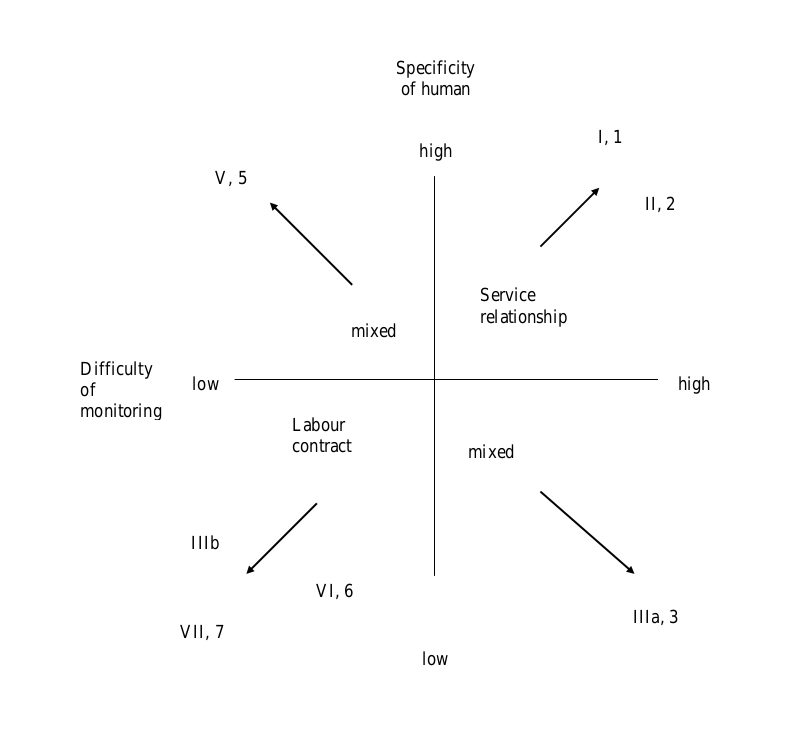
\includegraphics[width=\textwidth]{fig/Goldthorpe_ansaettelseskontrakt.png}
	\caption{Dimensioner af ansættelseskontrakten i Goldthorpes klasseskema}
	\label{fig_teori_klasse_Goldthorpe_arbejdskontraktdimensioner}
\end{centering}
\end{figure}

Den vertikale akse er specificiteten af kompetencerne, og kræver ikke yderligere forklaringen end den allerede givne.

Den horisontale akse, derimod, er udtryk for kontrollen over arbejdsprocessen. På venstre side er arbejdet af en sådan karakter, at dets udførsel og produktivitet let overvåges. Typisk vil det være manuelt arbejde.   
Til højre side findes arbejde, hvis karakter gør det svært at overvåge, og som ofte er service- relateret, eller har en symbolsk karakter, hvilket gør dets værdi og udførsel sværere at vurdere og overvåge. 

Det ses, at i det nederste venstre kvadrat gør kombinationen af højt udbud af færdigheder og nem monitorering en bestemt ansættelseskontrakt oplagt, \emph{arbejdskontrakten}. Det betyder at ansættelseskontrakten tilnærmer sig arbejdskraft som ren vare, da det er muligt at bestemme dens værdi ganske nøjagtigt. Dette er naturligvis den optimale situation set ud fra en arbejdsgivers synspunkt, og vil ofte indebære timelønning eller akkordlønning. Dette er arbejderklassens lod på arbejdsmarkedet. % skriv mere her når du gider, fx det med korter fyringsvarsler, mere som arbejdskraft man køber og sælger når man har brug for det. FX kan man se på skemaet at det der adskiller klasse IIIa og IIIb er at det er svært at overvåge arbejdet, men det er rutinepræget på en sådan vis at det er lige uspecifikt i kompetencer. Så grunden til at IIIa er så højt, er argumentet, at det er svært at overvåge deres arbejde.

I øverste højre kvadrat findes hvad Goldthorpe kalder ansættelseskontrakt som \emph{servicerelation}. De specifikke færdigheder giver gode muligheder for at forhandle gunstige arbejdsvilkår, og den diffuse målbarhed  kræver en incitatementsstrukturer, så lønmodtageren føler sig ansvarlig for firmaets mål. Dette er hvad hvad Goldthorpe kalder serviceklassen, eller \emph{salariatet}%
%
\footnote{Det kan være fornuftigt at benytte termet salariat fremfor serviceklasse, da det sidste kan forveksles med den slags repetitivt servicebaseret arbejde, der findes i dele af arbejderklassen og den lavere del af middelklassen, hvilket ikke er meningen: Salariatet er de to lønmodtagerklasser, der er \emph{mest} økonomisk begunstigede.}%
%
 \parencite[22]{GoldthorpeMcKnight2004}. %skriv mere når du gider hvis du gider at du gider

I disse to kvadrater kan man altså tale om, at selve arbejdets karakter giver enten arbejdsgiver eller arbejdstager fordele i forhandling af ansættelseskontrakten. I de to øvrige kvadrater er der tale et et blandet magtforhold, og der vil derfor være tale om et miks mellem de to typer ansættelseskontrakter. 

Ud fra disse to diffenteringsprincipper, baseret på bestemte arbejdsvilkår,laver Goldthorpe et klasseskema med 11 kategorier. Det er ud fra disse principper for arbejdsdelingen, der er grundlaget for magtpositioner, som de kommer til udtryk i ansættelseskontrakten. Ud fra disse udgår den sociale relation, en given arbejdstager har til produktionsmidlerne. % når analysen af Goldthorpes klasseskema er lavet med moneca, vurder hvor meget du skal skrive om hans klasseskema specifikt. FX det også kan kollapes til færre.


\label{klasse egp11}



Man kan sammenfatte Goldthorpes forståelse af hvad klasse \emph{gør} på følgende vis: 
%
\begin{enumerate}
 \itemsep-0.3em 		
 	\item Forskellige begivenheder indtræffer med forskellig styrker alt efter klasseposition
 	\item Forskel i interessedrejning hos forskellige klasser
 	\item Omkostninger forbundet med at forfølge en given interesse
\end{enumerate}
%
(Goldthorpe i \parencite[93]{Harrits2014}). Goldthorpe ser klassehandlen som  udtryk for de rationelle handlinger, et individ i en bestemt situation vil være tilbøjelig til at træffe. En rationel handlen defineres ud fra de økonomiske omstændigheder, individerne befinder sig i. I Goldthorpes fortolkning af økonomiske omstændigheder, vil det sige forholdet til produktionsmidlerne. Goldthorpe trækker på nymarxisten Jon Elsters forståelse af klassebaseret handlen som rationelle kollektive handling: Forskelle i belønninger kontra risici kan forklares ud fra sammenlignelige ressourcer i bestemte typer job. Især to forhold: Forskelle i begivenheder, der indtræder med forskellig styrke for forskellige klasser, fx arbejdsløshed, leder til \emph{ens}, men ikke nødvendigvis \emph{fælles}, handlingsmønstre indenfor klassen. individer i arbejderklassen have større risiko for arbejdsløshed, hvilket har betydning for den økonomiske sikkerhed, der findes i tilværelsen. Et andet eksempel er den økonomiske stabilitet, man kan forvente: i hvor høj grad et individ kan regne med, at lønindkomst er forudsigelig fra år til år, eller måned fra til måned, endda fra uge til uge \parencite[6, 10]{GoldthorpeMcKnight2004}.

Det andet: de transaktionsomkostninger og risici, der er forbundet med at forfølge bestemte mål, vil være ens, hvilket vil påvirke adfærd for individer i samme klassesituation. Børn fra mindre privilligerede familier vil have tendens til at satse på erhvervsrettede, kortere uddannelser, da afkastet i en sådan livsinvestering ikke kræver en risikabelt høj indsats, og sandsynligheden for en succesfuld sikring af klasseposition er høj, i deres position. 

Disse økonomiske forhold udgør en økonomisk virkelighed, som er ens for individer i samme klasseposition. Goldthorpe mener, at der i disse sammenhænge findes økonomisk rationelle strategier, som individer derfor vil have tilbøjelighed til at agere efter. Her understreger han, at i en given klassehandlen - altså kollektiv organisering for en gruppe lønmodtagere - kan det meget vel være mere rationelt at søge en korporativistisk fremfor antagonistisk strategi \parencite[215]{Goldthorpe2002}. Goldthorpe er ikke marxist, hvilket også ses i den forstand at han ikke anser \emph{en bestemt} type politisk handling som den objektivt rationelle, hvilket RAT-orienterede marxister har for vane at gøre (find henvisning til Boehmer, Wright, og ham fra Norge whats-his-face \#todo). Den danske velfærdsstatsmodel er eksempel på dette, hvor fagforeninger har anset det som mere fornuftigt at forfølge en overordnet korporativistisk strategi gennem det 20. århundrede. % referer til den der DSS bog? \#todo
% (Harris s. 93, hun citerer Goldthorpe 2000, find den og læs det (sociology and numbers hedder det vist, find det) \#todo

Overgang kunne være Oesch der citerer Goldthorpe for at se disse trends, men ikke mene at de er betydningsfulde endnu. (Oesch s. 28)


%%%%%%%%%%%%%%%%%%%%%%%%%%%%%%%%%%%%%%%%%%%%%%
\section{Daniel Oesch og arbejdslogik  \label{sec_}}
%%%%%%%%%%%%%%%%%%%%%%%%%%%%%%%%%%%%%%%%%%%%%%

Daniel Oesch er en schewizisk sociolog, der har søgt at reformulere et nyt grundlag for et klasseklassifikationsskema. Som hos Goldthorpe er udgangspunktet for klassedelingenden sociale relation til produktionsmidlerne, operationaliseret til erhvervsbeskæftigelse. 


Oesch mener at der sket så væsentlige ændringer i klassestrukturen, siden de mest benyttede klassifikationsskemaer blev lavet i 70'erne og 80'erne, af Wright og Goldthorpe. Denne periode var slutningen på hvad han kalder kapitalismens “gyldne æra,” og indfanger ikke klassestrukturen, som udviklingen har ført med sig, til et samfund delvist baseret på “postindustriel” produktion. Til forskel fra Daniel Bell (reference her \#todo), der forudså udviklingen af et postindustrielle samfund som en positivt betonet rationalisering og meritokratisering af samfundet, der førte til en opløsning af klassesamfundet, antager Oesch ikke en sådan udvikling. For Oesch betyder udviklingen af en offentlig sektor, kvindernes indtog på arbejdsmarkedet og  væksten i antallet af servicejobs, at klassekompositionen har \emph{ændret} sig, ikke opløst sig. Det er denne ændring, han vil indfange med sit klassifikationskema.  

Den bredere historiske analyse af årsagerne til denne ændring springer jeg let henover.

Man kan sige meget om årsagerne til disse udviklinger: Tænkere som Deleuze, Baumann, Adorno, (ham med netværkssamfundet), Negri \& Hardt, Richard Florida, Peter Wagner, Bourdieu m.m.fl. har forsøgt dette i mange år. Her vil jeg først redegøre for de tre tendenser, Oesch ser som væsentlige for at forstå ændringen i klassestrukturen. Dette sker kortfattet og hver tendens for sig. Derefter vil jeg gå lidt mere i dybden og forklare, hvordan samspillet mellem disse tre kommer til udtryk i en ændret klassestruktur, og hvordan Oesch mener at indfange denne struktur i sit klassifikationsskema. 

%
\subsection{årsager til ændringer i klassekompositionen \label{  subsec teori klasse Oesch aarsager}}
%


%
\subsubsection{tre årsager}
%


% industri- og serviceerhverv vækst findes der danske tal? \#todo

I forklaringen af den ændrede klassestruktur peger Oesch på 3 tendenser, der i perioden fra 70'erne og frem slog igennem i moderne vestlige samfund. Oesch viser udviklingen i disse tre tendenser, som de ser ud for Sverige, Tyskland, England og Schweiz \parencite[30]{Oesch2006a}.

Den første tendens er at den tertiære sektor/servicesektoren er vokset. Det betyder ikke kun flere jobs med høj specialiseret faglighed, det betyder også en vækst i antallet af servicefag med relativt lave uddannelseskrav. med andre ord sker er der sket en betydelig differentiering ud i forskellige typer af ikke-manuelle jobs. Dette ændrer på forholdet mellem manuelt/ikke-manuelt arbejde, hvor ikke-manuelt arbejde ofte automatisk har indebåret bedre vilkår end manuelt arbejde. Det mener Oesch ikke længere er tilfældet, og dette har ændret selve klassestrukturen \parencite[47]{Oesch2006a}. 

Den anden tendens er kvindernes indtræden på arbejdsmarkedet. I sin diskussion af Goldthorpes skema citerer Oesch Goldthorpe for at vedstå sig, at mange kvinder netop befinder sig i hans \texttt{klasse IIIb: lowergrade (hvad hedder det på dansk? find Harrits ord for det \#todo) rutinepræget ikke-manuelt arb.} \parencite[44]{Oesch2006a}. \texttt{Klasse III} benævnes samlet set som en slags “mellemposition”, eller middelklasse. Denne er karakteriseret ved at have en lav grad af “\emph{klassehed}” i sig; det vil sige, den fungerer som en slags residualkategori for serviceerhverv, der ikke har en høj status grundet uddannelsesmæssige specifikationer, eller i Goldthorpes jargon: sjældne kompetencer (det hedder det ikke men hvad hedder det så \#todo). Det er i høj grad kvinder, der fylder denne kategori, og Oesch mener at en nytænkning af klassifikationslogikken er nødvendig, for at tage højde for den permanente gruppe af servicebaseret, rutinepræget og primært \emph{kvindelig}, arbejdskraft, der er lokaliseret her \parencite[45]{Oesch2006a}. 

Den tredje tendens er ekspansionen og det generelt højere niveau af uddannet arbejdskraft. Det gælder også indenfor de traditionelt lavtuddannede - eller helt uuddannede - manuelle erhverv og de mange nye lavtløns jobs i servicesektoren. Det er især i de ikke-universitetsbaserede, erhvervsrettede serviceerhverv, at ekspansionen har været kraftig, ifølge Oesch (find henvisning \#todo)

Goldthorpe baserer sit skema på samfundet som det så ud i 70'erne, og siger selv, at hans formål ikke har været at forudsige tendenser i økonomien \parencite[48]{Oesch2006a}, men lave et klasseskema baseret på den nuværende økonomiske struktur. Oesch argument er, at disse tendenser ikke længere er tendenser, men \emph{er blevet} til den nuværende økonomiske struktur i (sen)moderne vestlige samfund. 

%
\subsubsection{Det ambigiøse i den automatiske hierarkisering af ikke-manuelt arbejde over manuelt}
%

For Oesch fører disse tre tendenser til en nuværende klassestruktur, hvor den traditionelle hierarkiske placering af ikke-manuelt arbejde over manuelt arbejde ikke længere er farbar; Det er ikke en hierarkisering, man kan tage for givet. Eller som Croutch siger det: “\emph{There are no grounds for regarindg the lower levels of the non-manual hierarchy as somehow superioer to manual work}” (ref \#todo) 1999:165. 

De lavtrangerende servicejobs inkluderer eksempelvis ikke den middelklassestatus, der ifølge Oesch tidligere var associaseret med ikke-manuelt arbejde. Disse servicefag har ofte en høj andel af kvinder, hvilket har betydning for deres placering på arbejdsmarkedet og dettes hierarki.   Sammenhængen mellem klassestrukturen og andre dybtliggende sociale strukturer såsom køn eller etnicitet bliver tydelig: Det er ikke et tilfælde, at arbejdsmarkedssegmenteringssteorien i USA er så optaget af den afroamerikanske befolknings placering på arbejdsmarkedet. Dette har ikke samme relevans i Danmark og andre nord- og vesteuropæiske lande%
%
\footnote{  I forbindelse med østudvidelsen af EU har vi set en diskussion af etnicitet særligt indenfor byggebranchen, restaurationsbranchen og rengøringsbranchen, og naturligvis også i diskussionen af indvandring fra ikke-vestlige lande. Min påstand vil dog være, at selvom dette påvirker visse brancher, og ikke er uvæsentligt, har det på ingen måde et omfang i Danmark, eller andre nord-og vesteuropæiske lande, der kræver en nytænkning af klassifikationslogikken som helhed. I modsætning til USA, hvor det forståeligt nok optog klasse-og arbejdsmarkedssegmenteringsteorietikere en hel del}%
%
. Det er muligt dette ændrer sig i fremtiden, og/eller allerede er på vej, som eksempelvis Mattias Tesfaye påpeger (henvisning \#todo). Kønsopdelingen af beskæftigelsesstrukturen og servicefagenes indlejring har dog en hel del flere år på bagen i de føromtalte samfund. Jeg vil formulere det således:
1) Den velkendte strukturelle placering af kvinders pligter/arbejdsområder under mænds i den traditionelle arbejdsdeling i hjemmet, gentages på arbejdsmarkedet i den samfundsmæssige arbejdsdeling, efterhånden som velfærdsstaten gradvist har overtagelet af en række af disse arbejdsopgaver op igennem den sidste halvdel af det 20. århundrede.2) Servicebaserede, rutineprægede erhverv såsom sekretær-relateret, adminstrativt arbejde, samt kundebetjening, har historisk set beskæftiget kvinder, og en vækst i efterspørgslen efter denne type jobs, bærer fortsat præg af dette. 

Det er ikke min - eller Oesch - påstand at dette udelukkende er kønsrelateret, og det er derfor jeg laver ovenstående skelnen mellem  traditionelt husarbejde og traditionelt servicearbejde. Det bliver interessant at se på, om eller hvorledes dette gør sig gældende på det danske arbejdsmarked. 

Nøglen er, ifølge Oesch, at lave en teoretisk konsistent klassifikation, således at skellet mellem manuelt/ikke-manuelt arbejde ikke per automatik medfører en vertikal placering af det sidste over det første. Dette skift i klassesstrukturen vil man have tilbøjelighed til at overse, hvis man benytter \emph{husstanden} som observationsenhed for klasseposition. Dette er ikke i sig selv en fejl, det kommer an på hvad der skal undersøges; Mere om det i afsnit REF \#todo. Men eftersom man i disse undersøgelser tit har taget mandens klasseposition som mål for husstanden, ser man, ifølge Oesch, ikke det føromtalte skift i klassestrukturen klart, da mandlige beskæftigede i langt højere grad stadig følger den vertikale placering af manuelt arbejde under ikke-manuelt arbejde \parencite[42]{Oesch2006a}.

Denne ambiguitet mellem “håndens og åndens” arbejde skyldes ikke kun væksten i antallet af rutineprægede servicejobs, men hænger sammen med en uddannelsesmæssig opgradering, også af den industrielle arbejdsstyrke. Denne opgradering har betydning både i toppen og bunden af arbejdsmarkedet: I bunden af arbejdsmarkedet
%find henvisning til snak om "den fjerde industrielle revolution"
reducerer uddannelsesvæksten/inflationen den sociale afstand mellem “bluecollar” \emph{arbejdere} og “whitecollar” \emph{ansatte(?!?)} . Distinktionen mellem arbejder og ansat er blevet mindre markerede, peger flere undersøgelser på \parencite[49]{Oesch2006a}. 

I toppen af arbejdsmarkedet kritiserer Oesch Goldthorpe for at betragte servicekontrakten til arbejdsgiveren som et homogent udtryk for \emph{én forenet} horisontal position indenfor serviceklassen%
%
\footnote{ Kun horisontalt, ikke vertikalt: Som beskrevet på side \pageref{klasse egp11} opdeler Goldthorpe selv serviceklassen i forhold til specifiteten af kompetencer, i en øvre og en nede serviceklasse.}%
%
 Goldthorpe insisterer på denne horisontalte enhed i serviceklassen, da han ingen teoretisk konsistent begrundelse har for en horisontal distinktion. Det kritiseres af Oesch for at være \emph{“somewhat academic”} \parencite[53]{Oesch2006a}. Med andre ord: Teoretisk stringens sættes højere end de differentieringer på arbejdsmarkedet, Oesch mener Goldthorpe dermed udelukker fra sit klasseskema.





 Denne forskel er på ingen måde så uskyldig som den lader til at være: faktisk åbner den netop den can of worms, som Oesch selv hævder han gerne vil lukke, når han fx siger han eksplicit vil betragte økonomiske klasser. Men det er jo netop det, Goldthorpe holder fast i her, og som Oesch så alligevel ikke mener er tilstrækkeligt. Det er ikke nødvendigvis et dårligt argument for uholdbarheden af rene økonomiske klasser, desværre præsenteres det ikke sådan af Oesch, der tværtimod - måske uden helt at være klar over det, eller ihvertfald uden at drage konsekvenserne vidtrækkende nok - først vil holde sig udelukkende til økonomiske klasser, men her reelt bryder med netop dette. Og, ironisk nok, uden at omtale det sådan, kritiserer Goldthorpe for netop at holde sig \emph{indenfor} de grænser, han selv siger må være horisonten for et udelukkende arbejdsmarkedsorienteret klasseskema! 






 Dette skyldes at Goldthorpe ikke vil 


ifølge Oesch, for at 



For det tredje er det tidligere omtalt \emph{salariat} øget i såvel antal som i heterogenitet. Det gælder både hvad Oesch kalder de management-lignende beskæftigelser samt de mere klassiske professioner%
%
\footnote{Professionerne skal her forstås i samme forstand som hos Goldthorpe på s. \ref{professionerne_def} \#todo}%
%
. De tre nævnte effekter i form af højere uddannelse%
%
\footnote{Eller,  med dansk uddannelsesforsknings \emph{grand old man}, Erik Jørgen Hansen, uddannelses\emph{inflation} find henvisning fra dds \#todo}%
%
, vækst i den tertiære sektor samt udviklingen af den offentlige sektor har haft en effekt inden for sammensætningen af disse middelklasser, omend - naturligvis - med andre effekter end på de andre to typer klasser. I væksten af velfærdsstaten ser Oesch det eksempelvis ikke køn som en central akse, som han gør det i de lavere serviceerhverv \parencite[2f]{Oesch2006a}. 
Denne forskel i betydning af det offentliges vækst for henholdvis de lavere servicefag og salariatet, argumenteres der ikke direkte for. Mellem linjerne kunne man sige at der ikke er tale om traditionelt kvindearbejde 

Resultatet er en klassestruktur, hvor sammenhænge mellem politiske holdninger, livsstil og økonomi har en anden dynamik end tidligere, hvilket alle klasseteoretikere mig bekendt anerkender (se Scott, Grusky, Harrits, Carsten etc etc find henvisninger \#todo). Eksempelvis gør salariatets heterogenisering det umuligt at behandle som en monolitisk størrelse, under een betegnelse såsom \emph{middelklassen}, eller evt. todelt til \emph{højere} og \emph{lavere} middelklasse, som vi ser hos Goldthorpe. Selvom Goldthorpe, som beskrevet på s ?? (\#todo) har yderligere opdelinger, er Oesch ikke overbevist om at dette er tilstrækkeligt for at forstå hvor forskellige de positioner, salariatet optager, egentligt er. Han mener der kræves ikke bare en \emph{empirisk} findeling, men en \emph{teoretisk} nytænkning af klassestrukturens diffenteringsakser i disse senmoderne, delvist postindustrielle samfund. 

\iffalse
\label{iffalse}

Oesch minimale klassedefinition: similarity in the position within the occupational system \parencite[16]{Oesch2006a}
 	→ AHA! men hvordan defineres position! Jeg har et bud hehehehe og det er anderledes end Oeschs hehehehe.

Breen: The major origin of data of class still rest on the golden age of capitalism  (oesch 1996, 16), s1 (nederst)

Økonomisk klasse: deler latente interesser i form af ens økonomisk situation, og ikke nødvendigvis meget andet. I modsætning til social klasse, der har større krav til identitet og ens organisering.  sæt evt. bourdieu what makes a class ind i den diskussion, for at kunne skille tingene ad. . wuhuu det blir godt. Eller Scotts distinktion mellem "social class" - household etc, og så klasseposition - individets klasseposition (refer til Scott 1994 ligesom Oesch gør det, s. 13)





klasse III i EGP består i høj grad af kvinder, og har i sin "intermediateness" et problem - måske er vi kommet langt nok i udviklingen af dette som en fast bestanddel til at kunne dekomposisere den? Lavet om til IIIb og IIIa netop af denne grund. Men er det nok? s. 46 vist nok

manual/non-manual ser ikke ud til at være brugbart rent hierarkisk s. 47-8. Ellers noget man har gået meget op i med fx. Lukacs. Darhendorff ser ud til at være mere brugbar

Bourdieu ser ikke ud til at være den bedste til at forstå det her ud fra. 

en udvidelse af en række jobs, hvilket man ser i jobs som s.49 - det finder jeg også!




Bruge arbejde eller markedssituation?
	→ klart reduktionistisk, me måske nødvendigt for at skabe sig et overblik. I dunno.

lav exceldata også på Oesch og Goldthorpes skema. Do it now!!! 




ps der er gratis kokain til de fem første!





artiklen om Trumps hvide arbejdervælgere. Brug den som argument for magten i klasseanalyse!


Goldthorpe laver, ligesom Weber, en skelnen mellem social klasse og social \emph{status}. Det 



s. 10 individuelle og strukturelle faktorer 



Det er ikke nødvendigvis sådan, at alle individer indenfor samme klasse forfølger samme interesser. Snarere sådan at individer i samme klasseposition vil have større affinitet overfor de samme interesser. Goldthorpe benytter Webers forståelse af social orden, forbundet med ære og hierarkisk værdisætning, som selvstændig kilde til social stratifikation og livsanskuelse. Disse værdisæt har ifølge Goldthorpe antaget en løsere form som det 20. århundrede skred frem, uden at det dog ser ud til at opløse dets effekter - snarere er denne form for “verdensanskuelse” langt mere betydningsfuld for at forstå eksempelvis kulturforbrug, og de politiske holdninger på en værdipolitisk akse, gående fra liberitær til autoritær (Goldthorpe i \parencite[95]{Harrits2014}. 

Selvom Goldthorpe understreger denne sociale status kilde til at forstå individerne og deres subjektivitet, er hans EGP-klasseskema dog strengt baseret på position på arbejdsmarkedet, da han laver denne skelnen mellem de to niveauer \parencite[95]{Harrits2014}. 








 









Det vil jeg gøre med følgende fremgangsmåde. 

Først vil jeg gennemgå Marx, der definerer relationerne til produktionsmidlerne som afgørende, og den udbytning, de danner basis for, og som definerer de sociale relationer. Derefter vil jeg gå ind i nymarxisternes hovedpine med basis-overbygningsmodellen, eftersom klassesamfundet ikke blev polariseret i to store klasser, sat imod hinanden, men i stedet fremkomsten af nye middelklasser samt nye serviceerhverv, der ikke ser ud til at være midlertige, men tværtimod helt nødvendige dele af den moderne kapitalisme. Jeg vil slutte min gennemgang af marxismens bud på stratifikation på arbejdsmarkedet ved det for mig at se mest empirisk anvendelige bud Eric Olin Wrights klassemodel.

Derefter vil jeg kort gennemgå Weber, der skelner mellem social status, klasse og stænder. Han har inspireret John Goldthorpes meget anvendte såkaldte EGP-klasseskema, der vil blive gennemgået som det næste, med dets fokus på kontrol over arbejdsprocessen og specifiteten af faglige kompetencer som de centrale differentieringsmekanismer. Goldthorpe har en analytisk-teoretisk funderet klasseforståelse, som bliver udfordret af David Grusky, der er fortaler for en noget anderledes klasseforståelse, baseret på erhvervsgrupper og de reelt oplevede fællesskaber, der findes her. Han benytter sig af Frank Parkins begreb om sociale lukningsmekanismer, som også bliver gennemgået (til Jens: sikkert for grundigt gennemgået, skal skæres til). I forhold til MONECA er hans bud spændende, da han udfordrer ideen om store klasser, og er fortaler for disse mikroklasser, som han mener drukner i de i sammenligning grovkornede klasseinddelinger, baseret på teoretiske principper. For mig at se kan Moneca netop være en måde at opdele i større klasser, baseret på empiriske bevægelsesmønstre, det vil sige give plads til Gruskys anke mod "big classes", som for mig at se er fornuftig nok, i og med en undersøgelse på mikroniveau kan afsløre klassedynamikker man ikke fanger på et højere plan. Jeg synes dog Gruskys teoretisk grundlag og affejning af teoretiske klasseinddelinger er problematisk, og hans afvisning af at der findes effekter af at tilhøre større klasser end erhvervsgrupper er problematisk. Her er Moneca en metode, der nærmest virker som skabt til at fungere på begge niveauer, det vil sige som beskrivelse af erhvervsgrupper på meget detaljeret niveua, samt mulighed for at afdække fællestræk i deres "sociale processer" på segmentniveau.

%til sidst vil jeg lede det over i metodeafsnittet, da både Grusky og Goldthorpe benytter økonometrisk funderet regressionsanalyse, og jeg vil mene at en relationelt funderet social netværksanalyse har mulighed for at klasser som relationelle størrelser, fremfor som udtryk for variable.



%DET VIL JEG VIL GØRE MED FØLGENDE FREMGANGSMÅDE...

% Forskellige bud på klasser
% 	Marx
% 		-forholdet til produktionsmidlerne, udbytning
% 	Nymarxisme	
% 		- Problemerne i basis-overbygning og middelklassens position
% 		- Redskaber mere nuancerede end kapital-arbejde - hvordan, og stadig beholde den marxistiske kerne? 
% 	Wright
% 		- klasse som forklarende og nominel (tror jeg)
% 		- Tre dimensioner: Ejerskab over produktionsmidler, autoritet, færdigheder
% 	Weber
% 		- Klasse, social status og stænder
% 	Goldthorpe
% 		- Klasse som forklarende og nominel
% 		- Tre dimensioner: Ejerskab over produktionsmidlerne (knapt så centralt), specifiteten af kompetencer, kontrol over arbejdsprocessen 
% 	Grusky
% 		- Klasse som beskrivende og realistisk
% 		- kritik af nominel klasseinddeling
% 			- for grovkornet
% 			- misser det centrale ved definition udenfor de reelt oplevede fælleskaber
% 		- erhvervsgrupper som klasser, sociale lukningsmekanismer

%DET SKAL ALT SAMMEN BRUGES TIL...

	% Opsamling: 
	% 	- Kobling til delanalyse 1: Moneca som måde at inddele arbejdsmarkedet i segmenter (klasser)
	% 	- Kobling til delanalyse 2: Forklare sociale processer i segmenter (klasser) vha. klasseforskere
	% 	- Kobling til delanalyse 3: Jeg  placere Moneca som et oplagt bud på at mediere og vurdere de to positioner (den realistiske og nominelle klasseindling)

Denne teoretiske gennemgang skal bruges til følgende i forbindelse med det overordnede spørgsmål om arbejdsmarkedets segmentering, i 3 analyser:

\begin{itemize}
  \item Delanalyse 1: Moneca som måde at inddele arbejdsmarkedet i segmenter
  \item Delanalyse 2: Forklare sociale processer i segmenter (klasser) vha. klasseforskere
  \item Delanalyse 3: Moneca som på at mediere og vurdere de to positioner (den realistiske og nominelle klasseindeling hos henholdsvis Grusky og Goldthorpe)
\end{itemize}



%Motivation for at inddrage klasseteori er, at analysen af delmarkeder/segmenter og mobilitet ligger inden for en tradition af klasseteori. Dette ses såvel i Wrights analyse/teori om bla bla bla såvel som i Gruskys analyse/teori om...

%Arbejdsmarkedssegmenteringsteorien, som ligger til grund for Toubøl, Larsen og Strøbys udvikling af en a posteori arbejdsmarkedssegmenteringsanalyse, ligger inden for en amerikansk/anglo-saksisk økonomisk diskussion op i mod den neoklassiske økonomiske teori \parencite[2]{Touboel2013}. Thomas Boje opsummerer kritikkken således:

%\begin{displayquote} “\textit{The core of this criticism is first that neoclassical labour-market theories in their analogies to the commodity market do not take into account the heterogeneous character of the labour market and the lack of homogeneity in the labour force. Secondly the theories do not take into account that the behaviour of individuals on the labour market is not governed by economic utility maximization, but, on the contrary, determined by social relations and institutions of which the individual is an integral part.}” \parencite[171]{Boje1986}. \end{displayquote}

%Segmenteringsteorien fremkomst primært i USA opstod ifølge Cain i 1960'erne og 1970'erne som en reaktion på kampen mod fattigdom og fuld deltagelse i økonomien for blandt andet minoritetsgrupper og kvinder \parencite[1216]{Cain1976}. Doeringer og Piore opdelte arbejdsmarkedet i primære og sekundære markeder med “gode” jobs og sidstnævnte indeholder alle de “dårlige” jobs med henblik på at forklare den ulige fordeling af lønninger \parencite[70]{Doeringer1971}, mens Reich, Gordan og Edwards mere radikale tilgang tilgang beskrev, hvordan den historiske proces, hvorved politisk-økonomiske kræfter fremmer opdelingen af arbejdsmarkedet i seperate delmarkeder \parencite[359]{Reich1973}. Hvor denne segmenteringsteori tager udgangspunkt i forandringerne i sin tid og en økomisk kritik af økonomien, så er mit udgangspunkt og fokus et andet. Mit udgangspunkt er den sociologiske tradition, klasseteori og klassediskussion.

%Derfor vil jeg frem for at dykke ned i segmenteringsteoretikerne tage fat i de sociologiske klaseteoretikere såsom Marx, Weber, Gitte Harrits, Goldthorpe, Wright, Parkin og Grusky. Disse teoretikere er både med til at forklare det første kritikere i forhold til delmarkeder og mobilitet (fx Weber og Goldthorpe), hvilket var bla bla bla... Samtidig ligger der også inden for andet kriterie det vil sige, hvorfor der er forskellen på et delmarked og et segmenter er forskelle i sociale processeser (fx Wright og Goldthorpe). Alt sammen er det interessant også for det tredjhe kriterie oim hvorfor sociale processer fører til segmentering.




%%%%%%%%%%%%%%%%%%%%%%%%%%%%%%%%%%%%%%%%%%%%%%
\section{Karl Marx \label{2_marx}}
%%%%%%%%%%%%%%%%%%%%%%%%%%%%%%%%%%%%%%%%%%%%%%

Marx selv nåede aldrig at færdiggøre sin klasseteori, eller skitsere den i en sammenhængende form. Kapitel 52 i tredje bind af \emph{Kapitalen} har titlen "Klasserne", men efter cirka en side stopper skriften, og Engels, der udgav værket efter Marx' død, skriver: "Her afbrydes manuskriptet" \parencite[22]{Harrits2014}. Som samlet klasseteori må man derfor benytte sig af Marx' generelle teoriapparat, for at forstå hvad en klasse er hos Marx. Det er værd at huske på, at netop fordi klasserne ikke nåede at modtage en specifik teoretisk behandling, må klasseteorien konstrueres ud fra hans generelle historieforståelse.

Formålet her er ikke en grundig gennemgang, men en skitsering, der skal tydeliggøre fundamentet i den neomarxistiske klasseforståelse.

Klasserne hos Marx er defineret ud fra den tilgang, at det vigtigste menneskelige forhold omhandler produktionen af livsfornødenheder, altså de materielle forhold. De værktøjer - forstået i bredest mulige forstand - som gør det muligt at producere disse livsfornødenheder, defineres som produktionsmidlerne. Menneskers forhold til produktionsmidlerne er dermed den centrale sociale relation i et samfund, og igennem denne primære sociale relatio udgår alle andre sociale relationer. Det vil sige, at mennesker med samme sociale relation, lad os kalde det ejerskabsforhold, til produktionsmidlerne, kan karakteriseres som en klasse, da de deler det mest centrale grundvilkår, nemlig betingelsen der tillader dem at reproducere deres livsgrundlag. Marx peger på det forhold, at mennesker er i stand til at arbejde mere, end det der skal til for at holde dem i live, og det arbejde, der ligger udover hvad der skal til for at reproducere dem som arbejdskraft, kaldes merarbejdet. Det er dette arbejde, der er grundlag for udbytningsrelationer mellem forskellige klasser, hvor nogle klasser i kraft af deres ejerskab over produktionsmidlerne kan nyde godt af de primære producenters arbejdskraft. Det er således både en dominansrelation og en udbytningsrelation på spil, i forholdet mellem de eller den herskende klasse og den eller de klasser, der tvinges til at arbejde for dem.

Kapitalistiske samfund er kort sagt karakteriseret ved, at penge bliver den centrale mediator mellem forskellige former for arbejde. Hvad enten den er indlejret som arbejdstid i en fysisk form som en stol, et kilo sukker, eller i et menneske, som levende arbejdskraft. Det er denne "universelle ækvivalent", som Marx kalder den, der tillader det moderne kapitalistiske marked, hvori alle former for menneskeligt arbejde kan udveksles frit som varer. Frit er det dog ikke helt, da det er Marx påstand, at kun en enkelt vare rummer en ganske særlig kvalitet, nemlig evnen til at avle mere arbejde end det, der er indlejret i den. Den vare er mennesket. Et kapitalistiske samfund er derved karakteriseret ved lønarbejde, hvori en klasse, borgerskabet, ejer produktionsmidlerne, mens størstedelen fungerer som den arbejderklasse, der bliver betalt mindre, end deres arbejde er værd, men nok til at reproducere deres arbejdskraft. Det er Marx forudsigelse, at i overgangen fra feudalsamfundet til det kapitalistiske samfund, vil størstedelen af feudalsamfundets udbyttede klasser blive tvunget fra at have, eller i det mindste være i besiddelse af, deres egne produktionsmidler, til at arbejde direkte for borgerskabet i form af løn. Det kapitalistiske samfund vil derfor blive karakteriseret ved en tiltagende polariseret klassekamp mellem arbejdere og kapitalister, bourgeosi og proletariat.

Det behøver ikke nødvendigvis tolkes sådan, at der findes to klasser, der empirisk stringent kan deles op, selvom det, særligt i mere polemisk og politiske øjemed, er blevet benyttet sådan. I Marx' egne konkrete klasseanalyser benytter han en række termer for klasser og klassefraktioner, ikke kun bourgeosiet og proletariatet. Snarere er påstanden, at der findes en grundlæggende modsætning mellem arbejde og kapital, og denne modsætning er afgørende for interesserne og handlemønstrene for dem, der står på henholdsvis den ene og den anden side af denne modsætning. Her benytter Marx sig af begreberne "klasse i sig" og "klasse for sig", hvor det første er en klasse, der findes objektivt, bestemt af de sociale relationer, og det andet er en klasse, der forstår sig selv som klasse. Der er altså to niveauer i en klasseanalyse:

- et abstrakt niveau, der handler om kampen om merværdi og den grundlæggende klassemodsætning i samfundet
- et konkret niveau, om de observerbare klassefraktioner og grupperinger, der indgår i de politiske kampe i samfundet \parencite[26]{Harrits2014}. %lav til liste

Marx' teori indeholder derfor, som Harris fremhæver, ikke nødvendigvis en påstand om arbejderklassens enhed, men kan ligeså vel tolkes som en invitation til at lave historiske analyser med fokus på samfundsforandring, klassedannelse og politiske magtkampe \parencite[28]{Harrits2014}. I den marxistiske tradition ligger der altså et fokus på at bestemme klasser ud fra deres forhold til produktionsmidlerne, sagt med lidt mere almindelige termer: Hvilken overordnet beskæftigelse, man er i. Den fokuserer derfor på relationer indenfor produktionen, og ikke markedsrelationer, med særligt fokus på den \emph{udbytning} der findes i disse relationer.


%%%%%%%%%%%%%%%%%%%%%%%%%%%%%%%%%%%%%%%%%%%%%%
\section{Problemet med middelklassen og det marxistiske svar \label{2_nymarxisme}}
%%%%%%%%%%%%%%%%%%%%%%%%%%%%%%%%%%%%%%%%%%%%%%

Ikke desto mindre udviklede de moderne samfund sig ikke sådan, at kapitalismens centrifugalkræfter delte samfundet i to, med kapitalister og arbejdere sat overfor hinanden, grundet deres ensartede relation til produktionsmidlerne, som besiddende og ikke-besiddende. Den basale to-klasse model synes ikke at fange de interessemodsætninger og klasseformationer, som opstod i stabile kapitalistiske samfund. En række klasser i det sociale stratum med ejerskab over egne produktionsmidler, såsom artians, small traders, shopkeepers and småbønder, %hvordan fanden oversætter man det
forsvandt godt nok (evt. Parkin henvisning). Men denne polarisering i den socioøkonomiske struktur - altså en koncentration af produktionsmidlerne i færre hænder - blev historisk ikke til to store klasser, sat i mod hinanden, og den teoretiske skillelinje fra den marxistiske politiske økonomi mellem arbejde - kapital kunne tydeligvis ikke omsættes til en tilsvarende opdeling i klasser med egentlig ageren efter denne opdeling. Det vigtige i denne afhandling er, at selvom denne modsætning mellem arbejde - kapital måske nok findes - som påvist af bl.a. Thomas Pikkety, og strukturerer indkomstfordeling på afgørende vis, fungerer denne grundlæggende struktur ikke på nogen entydig måde, der gør denne opdeling særlig brugbar til at undersøge de klasseformationer, vi kan observere empirisk. 

En række andre forhold må medtænkes, da det er tydeligt at middelklassen, der erstattede det gamle småborgerskab, ikke er ekstern i forhold til den kapitalistiske produktionsmåde, men er en central del af den, som Parkin påpeger i sit værk \emph{Marxism and Class Theory: A Bourgeois Critique} fra 1979 \parencite[16]{Parkin1979}. %kan man henvise bare til siden når værket allerede er nævnt?

Der må altså være en række forhold, der muliggør eksistensen af den langt mere komplekse klassestruktur i senmoderne, stabile, kapitalistiske samfund, og som er af central betydning for at forstå klasseformationerne i dette.

Hvis arbejde-kapital ikke er en skillelinje, der giver særlig meget forklaringskraft i de samfund, der findes, hvad gør man så, for at finde de politisk relevante brudflader mellem klasserne? Og hvad skal man gøre med den føromtalte middelklasse? Det er hvad Parkin kalder \emph{the boundary problem in Marxism and sociology} \parencite[11]{Parkin1979}. 

Parkin identificerer tre nymarxistiske svar på dette problem. De to første skal kun kort skitseres, mens den sidste, repræsenteret ved Eric Olin Wright, bliver gennemgået i dybden. 

Det første svar er, hvad Parkin kalder \emph{den minimalistiske} definition af arbejderklassen, repræsenteret ved Poulantzas. Her drages skillelinjen mellem produktivt og uproduktivt arbejde, baseret på en fortolkning af hvilken form for arbejde, der skaber merværdi. Lønarbejde, der ikke skaber merværdi, er også udbytning, og indgår derfor ikke i proletariatet, altså den politisk relevante samfundsgruppe i marxistisk optik. Det giver en forklaring på stabile udbytningsrelationer, også lønarbejdere i mellem. 

Det andet svar er den \emph{maksimalistiske} version, repræsenteret ved Poul Baran, der benytter sig af Marx' lighedstegn, visser steder i sine skrifter, mellem \emph{folket} og arbejderklassen. De mange mod de få. Her benyttes et politisk defineret kriterie baseret på hvilke sociale grupper, hvis sociale funktion også ville være nødvendige i et socialistisk samfund \parencite[20]{Parkin1979}. Det er politisk i den forstand, at det handler om at skabe forening mod en overklasse, og analytisk i den forstand, at det prøver at forudsige, hvilket arbejde der kan siges at være \emph{samfundsmæssigt nødvendigt}, for på den måde at klassificere dem, der lever af andres arbejde.  

Begge disse svar forekommer mig ikke særlig anvendelige i en konkret klasseanalyse, og nævnes derfor kun som forsøg på at løse “\emph{the problem of the middle-classes}”, som som Wright kalder det \parencite[15]{Wright2000}. I stedet vil jeg fokusere på den nymarxistiske retning Parkin kalder \emph{mellempositionen}, som Parkin karakteriserer ved Erik Olin Wright selv \parencite[17]{Parkin1979}.


%%%%%%%%%%%%%%%%%%%%%%%%%%%%%%%%%%%%%%%%%%%%%%
\section{Erik Olin Wright \label{2_wright}}
%%%%%%%%%%%%%%%%%%%%%%%%%%%%%%%%%%%%%%%%%%%%%%

Erik Olin Wright introducerer to dimensioner for at forstå hvad han kalder \emph{modsætningsfyldte klassepositioner}, normalt omtalt som middelklassen: “\emph{people who do not own their own means of production, who sell their labor power on a labor market, and yet do not seem part of the working class.}” \parencite[15]{Wright2000}. Det giver samtidig anledning til at differentiere arbejderklassen og klassesamfundet generelt, i en mere nuanceret klassebaseret stratifikationsteori, der viser \emph{hvad klasse gør}, som Harris formulerede det. 

Centralt står stadig forholdet til produktionsmidlerne og de udbytningsrelationer, der hersker mellem mennesker, alt efter deres relation til produktionsmidlerne. Wright sætter to dimensioner på udbytningsforholdet, der udtrykker mulighederne for at tilegnelse af samfundets ressourcer. Klassepositioner ses som udtryk for en kombination af disse to akser samtidig med, at han bibeholder overordnede skelnen mellem ejer-ikke ejer.

Den første akse kalder Wright \emph{autoritetspositioner}, og omhandler det forhold, at kapitalejere uddelegerer deres lovmæssige ret til at lede og fordele arbejdet til andre. Det sætter dem i en modsætningsfyldt klasseposition, da de ikke er kapitalister selv, men står over arbejderne, og modtager højere løn for deres ansvar i en virksomheds daglige ledelse. Den anden akse kalder Wright \emph{færdigheder}, der beskriver de faglige og tekniske færdigheder, der er nødvendige for en given produktion. 



 % Søren: Dette kan bruges i forhold til sociale processer i segmenterne på sammen måde som "socia closure".


Udover disse akser har Wright, traditionen tro fra Marx, en skillelinje mellem ejere og ansatte, altså de, der selv ejer produktionsmidler, og de, der ikke gør. Disse to akser demonstrerer dermed en skala af klassepositioner, der muliggør forskellige slags tilhørsforhold og identiter, der ikke nødvendigvis polariseres i den enkeltdimensionerede arbejder-kapitalist relation, omend denne grundlæggende modsætning bibeholdes i modellen. Middelklassen bliver dermed den gruppe mennesker, der befinder sig i disse mellempositioner, og Wrights model muliggør også at positionere ansatte indenfor service- og informations industrien, der traditionelt har voldt marxistiske teoretikere en del genvordigheder.

Wright benytter denne udbyggede model til at forstå, hvordan man på det samfundsmæssige plan ser bestemte klasseformationer og politiske kampe, der gerne skulle kunne forklares ud fra denne klassemodel. Spørgsmålet om hvorvidt man skal kortlægge klassestrukturerer “bag om ryggen” på individerne står altså stadig centralt. Wright fastholder på den side ene side en teoretisk model, baseret på udbytningsrelationer i økonomien, samtidig med at den konkrete udformning af denne skal testes empirisk og revurderes løbende, baseret på dens evne til at forklare politiske kampe og observerede klasseformationer s. 75. 

% brug evt. henvisning fra Harris s. 67 til to konkrete danske analyser med brug af Wrights klassemodel 


%%%%%%%%%%%%%%%%%%%%%%%%%%%%%%%%%%%%%%%%%%%%%%
\section{Max Weber \label{2_weber}}
%%%%%%%%%%%%%%%%%%%%%%%%%%%%%%%%%%%%%%%%%%%%%%

Selvom Weber heller aldrig nåede at færdiggøre sin klasseteori, fremstår den i noget mere færdig form end tilfældet er hos Marx \parencite[28]{Harrits2014}. Webers klasseteori medtager stratifikation, der ligger udover hans klassebegreb, og indeholder derfor en mere pluralistisk tilgang til samfundets opdeling i forskellige sociale grupperinger. Hans klassebegreb er dog tydeligt inspireret af Marx, i den forstand at det er bundet op på økonomiske interesser og et bestemt forhold til produktionsmidlerne:
%
\begin{displayquote} “\textit{Vi vil tale om "klasse" når 1. livsbetingelserne for en flerhed af mennesker er betinget af en specifik fælles komponent, for så vidt 2. denne komponent ene og alene udgøres af økonomiske ejendoms- og erhvervsinteresser, og det foregår på 3. (vare- eller arbejds)markedets betingelser ("klassesituation"}” \parencite[302]{Weber1978}. \end{displayquote}
%
Til forskel fra Marx er klasser også defineret ved deres status på arbejdsmarkedet, fremfor relationen til produktionsmidlerne, og der ligger derfor et større fokus på markedsrelationer, altså “\emph{arten af éns chancer på markedet}” (weber 31 2003, i \parencite[29]{Harrits2014}). For at begribe disse chancer på markedet, der jo i høj grad er bestemt af hvilken økonomisk klasse, man er i, siger Weber, at det er ens evne til at tilegne sig indtægter og goder (Weber 1976 i \parencite[29]{Harrits2014}). Det åbner op for et kulturelt perspektiv, da alle mulige egenskaber, der kan omsættes til økonomiske ressourcer, bliver en del af et menneskes livschancer på markedet. Hos Weber finder vi et klassebegreb, der i udgangspunktet indeholder en typologi baseret på ejerskab/ikke-ejerskab over produktionsmidlerne, men derudover indeholder en langt bredere forståelse af klassefraktioner indkapslet i konceptualisering af hvad der definerer klasser. Og i øvrigt ligger tæt på Marx egne konkrete analyser af klasser, som omtalt tidligere.

Weber peger også på mobilitet mellem klasser som et centralt spørgsmål for klasseforskning. Så bevæger vi os hen til at beskrive, hvad klasse \emph{gør} parencite[302]{Weber1978}. Der er hos Weber et større fokus på den subjektive oplevelse af klassetilhørsforhold. Selvom folk individuelt reagerer ens på deres klassesituation, er det ikke ensbetydende med en deterministisk bevægelse hen imod en klasse-for-sig, som hos Marx. Weber er dermed mere interesseret i alle de aspekter, som en klasse \emph{gør}, fremfor Marx fokus på politiske kampe og social forandring. Klassebegrebet kan bruges generelt til undersøgelse af interessekampe, mobilitet og al mulig anden adfærd. (Harris 31). % Søren: Dette skal du vende tilbage til i analysen - intern mobilitet som en weberiansk klasse-/segmentopdeling.

Det sidste centrale begreb hos Weber er hans begreb om stænder. Det vil sige hans forståelse af, at der udover en økonomisk orden, også er en social orden, "den måde hvorpå social ære" fordeler sig i et fælleskab" (Harris 31). Denne sociale orden er en \emph{selvstændig} kilde til magt i et fælleskab, hvilket er en væsentlig forskel fra den marxistiske klasseanalyse. Det er knyttet op på subjektive oplevelser af fælleskab og anerkendelse af bestemte former for livsførsel om særligt attråværdige. Selvom Weber understreger stænders selvstændighed i forhold til klassesituationen, bliver spørgsmålet om sammenfaldet mellem klasse og stænder, og den måde, de kommer til udtryk på i en bestemt praksis, et genstandsfelt for klasseforskning \parencite[32]{Harrits2014}.




%%%%%%%%%%%%%%%%%%%%%%%%%%%%%%%%%%%%%%%%%%%%%%
\section{Grusky og Parkin \label{gruskyogparkin}}
%%%%%%%%%%%%%%%%%%%%%%%%%%%%%%%%%%%%%%%%%%%%%%

Grusky har to kritikker af klasseanalyse som den almindeligvis bedrives: For det første at de er nominelt funderede, fremfor at tage reelt oplevede, sociale fællesskaber som grundprincip for klasseinddelingerne. Og for det andet, at de derved ender med en grovkornet klasseinddeling, der skjuler udbytnings- og stratifikationsmekanismer, der burde være i centrum af klasseforskningen. 

%brug eventuelt: basis skal være institutionaliserede, "aktøroplevede" (dårligt ord) erhvervsgruppers i samfundet. Det er på dette niveau, at klasse reelt "fungerer" (Grusky 2001 eller 2002 find henvisning)

Grusky påpeger at menneskers identifikation med klassebaserede identiteter historisk er blevet svagere og svagere, samt den manglende massehandlen, der burde følge med positioner i arbejderklassen, hvilket har ledt til en hel del \emph{nymarxistisk håndvridning}, som han kalder det \parencite[205]{Grusky2001}. 

Det er ikke problemet at benytte beskæftigelse som grundlag for klasseinddeling. Problemet er niveauet af aggregering, der sker ved at placere en lang række forskellige professioner i eksempelvis kategorien \emph{nedre serviceklasse}, som hos Goldthorpe, baseret på teoretisk funderede magtdimensioner, i Goldthorpes tilfælde: Kontrol over arbejdsprocessen samt specificiteten af færdigheder. 

Klasseanalyse bør tage udgangspunkt i hvad Grusky kalder \emph{realistiske} fælleskaber, altså fælleskaber der opleves som sådan af individerne i dem. Det er på dette (bevidste) niveau, at sociale stratifikationsmekanismer reelt opererer \parencite[212]{Grusky2001}. Det er ikke sådan, at den funktionelle enshed i arbejdet, som er fundamentet for erhvervsklassifikationsskemaer, skal tages for pålydende. Funktionel enshed i arbejdet er ikke nødvendigvis lig den sociale enshed, Grusky ser som udgangspunktet for en klasseanalyse. Han mener at denne "\emph{technicist vision}" %
\label{gruskytechnicistvision}%
også bør medtage reelt oplevede sociale distinktioner, fremfor udelukkende tekniske hensyn \parencite[215:fodnote 5]{Grusky2001}%
%
\footnote{Han nævner bl.a. ISCO, der benyttes af Danmarks Statistik, og som jeg også benytter i denne afhandling. Mere om det senere.}%
%
. Men på et tilstrækkeligt detaljeret niveau, hvor vi nærmer os rene professioner, er sandsynligheden for reelt oplevede fælleskaber størst \parencite[207]{Grusky2001}. Ud fra dette niveau kan aggregation i større klasser \emph{eventuelt} finde sted, omend man fornemmer at guldstandarden for Grusky stadig er de realistiske fællesskaber. Det er hans to validitetskriterier: Det første er at medlemmerne i den skal forstå sig selv som tilhørende en gruppe, baseret på beskæftigelse. Det andet er at kollektiv handlen, der sikrer denne gruppe privilegier, forstået som \emph{social luknings}-strategier. Det er et begreb fra Parkins professionssociologi, Grusky ser ud til at overføre direkte. Jeg vil derfor gennemgå Parkins definition af det nu. 

For Parkin er \emph{social lukning} som basis for gruppedannelse en måde at tilbyde et alternativ til den marxistiske nominelle klasseforståelse. Alternativet er baseret på en omfattende kritik af den særstatus, relationen til produktionsmidlerne har i marxistisk klasseinddeling. Især de ikke-holdbare krumspring, han mener nymarxister gør sig for at bevare denne særstatus, samtidig med at klasserne "ikke gør det, det var meningen de skulle gøre". Denne kritik vil ikke blive gennemgået nærmere, jeg vil i stedet fokusere på hans egen forklaringsmodel på stratifikation og udbytningsmekanismer. I forlængelse af den weberianske tradition mener Parkin, at en autoritet- og statussrelationer, der fungerer på niveauet af \emph{distributionen af goder} i samfundet er central. Det bør tillægges lige så stor vægt som ejerskabet til produktionsmidlerne \parencite[24f]{Parkin1979}. Dermed sidestilles markedsmuligheder og livschancer med den direkte relation til produktionsmidlerne%
%
\footnote{Parkin anerkender, nymarxister også har måtte indoptage denne dimension af klassekamp i deres teoriapparat. "inside every neo-Marxist there seeems to be a Weberian struggling to get out", som Parkin skadefro formulerer det. \parencite[25]{Parkin1979}. Man kunne også have sagt det omvendte, hvis man ville.}%
%
. Parkin er ikke interesseret i at revitalisere Webers klasseanalyse, men i at benytte den weberianske forståelse af sammenhængen mellem produktionsrelationer, symbolske relationer og markedseffekter, til foreslå et nyt framework til at forstå sociale gruppers kamp om goder i samfundet. Hans pointe er, at hvis man skal forstå sociale afgrænsninger, er (produktionsorienteret) klassebaseret afgrænsning kun en dimension, og det giver ikke mening at tillægge denne større vægt end andre historiske diffenteringsmekanismer, hvoraf han fremhæver etnicitet som et markant eksempel \parencite[38f]{Parkin1979}. Han vil derfor gerne skabe en teori, der kan rumme \emph{enhver slags} social afgræsning, i kampen om samfundets goder \parencite[42]{Parkin1979}. 

Parkin tager fat i Webers begreb \emph{social lukning} i fundamentet af denne teori. Han skriver:
%
\begin{displayquote} “By social closure Weber means the process by which social collectivities seek to maximize rewards by restricting access to resources and opportunities to a limited circle of eligbles. This entails the singling out of certain social or physical attribute as the justificatory basis of exclusion. (...) the nature of these exlusionary practices, and the completeness of social closure, determine the general character of the distributive system” \parencite[44]{Parkin1979}. \end{displayquote}
%
I samme åndedrag skriver Parkins, at tilegnelsen af økonomiske ressourcer er central \parencite[44]{Parkin1979}. Konsekvensen af ovenstående citat,for Parkins, er at udbytning ikke længere defineres som udtryk for en relation til produktionsmidlerne, men at ejerskab over produktionsmidlerne ses som en specifik, og dog helt central social lukningstrategi, der muliggør udbytning \parencite[53]{Parkin1979}. 

Parkins peger på en anden væsentlig kilde til udbytning i moderne samfund, som er de højere, bogligt funderede uddannelser%
%
\footnote{Parkin benytter den engelske betegnelse \emph{the professions}, hvilket jeg vil mene kan oversættes til ovenstående på dansk [er du enig Jens?]}%
%
. Ligesom en række andre sociologer såsom Bourdieu og Collins (\#henvisningmangler) peger Parkin på professionalisering gennem uddannelse og juridisk legitime uddannelsesdiplomer som central differentieringsmekanisme i moderne samfund, hvilket han kalder \emph{kredentialisme}. I Parkins teori er der tale om udbytning, da der tilegnes ressourcer i form af social lukning: En strategi til at hæve markedsværdien \parencite[54]{Parkin1979}. I Thomas Bojes optik kunne vi sige, at det er erhvervsgruppers måde at kontrollere udbuddet af arbejdskraft på et givent område, for dermed at øge markedsværdien. Parkin adskiller denne kredentialistiske strategi indenfor de længere uddannelser, med de strategier, fagforeninger bruger for at beskytte sig imod udbytning fra arbejdsgivere, da det bevidste mål ikke er at reducere de materielle muligheder for andre i arbejdsstyrken \parencite[57]{Parkin1979}. Dette vidensmonopol for de længerevarende uddannelser mener han er så omfattende, at overklassen i dag udgøres af ejerne og (deres ansatte) ledere af produktionsmidlerne, samt de lærde klasser med monopol en særlig viden \parencite[58]{Parkin1979}. 

Parkin skelner mellem social lukning som \emph{eksklusion}, hvor målet er at tilegne sig ressourcer ved at ekskludere andre, og social lukning som \emph{usurpation}. Det sidste foregår som respons på en i samfundet befæstet, muligvis \emph{formaliseret}, eksklusion. For eksempel organiserede lønarbejderes kamp for bedre løn og arbejdsvilkår, eller etniske gruppers kamp for udvidelse af deres juridiske borgerrettigheder \parencite[74]{Parkin1979}. 

Ekslusionsbaserede social lukningsstrategier er, som eksempelvis etnicitetsbaserede kriterier viser, ikke kun noget, der hører klasser som helhed til. Parkin peger også på eksklusitionsbaseret social lukning indenfor klasser, i hvad han kalder \emph{dobbelt lukning}. Han bruger arbejderklassen som eksempel, uden at definere den nærmere, men man antage at han mener de lønmodtagere, der ikke tilhører de professionaliserede højtuddannede. Disse benytter også eksklutionsbaseret social lukning mod andre dele af klassen. Det kan ske baseres på køn, etnicitet eller andre sociale kriterier der giver mening i den sociale kontekst \parencite[89]{Parkin1979}. Når en indfødt arbejderklasse lukker sig overfor en arbejderklasse fra et andet land, handler det ofte om at sikre de sikrede rettigheder overfor udvidelsen af arbejdsudbuddet til dårligere forhold \parencite[91]{Parkin1979}. Det virker ganske genkendeligt i diskussion af østarbejderes indtog í Danmark. Som han siger: "\emph{workers who opt for closure against a minority can hardly de beclared guilty of irrationality in choosing to retain the proven benefits of exclusion in preference to the uncertain or doubtful pay-off resulting from combined usupartion.}" s. 95". Ligeledes er fragmentering i klasserne langs beskæftigelsesmæssige linjer et vigtigt fokuspunkt \parencite[81]{Parkin1979}.

I en tilbagevenden til Grusky kan vi sige, at Parkin er helt enig i Gruskys 2. kriterie for klasseinddeling: For Parkin er kollektiv handlen det, der definerer en klasse, og ikke en a priori teoretisk inddeling, som han ikke har meget til overs overfor \parencite[113]{Parkin1979}. De skøjter simpelhen over potentielt vigtige lukningsmekanismer internt i deres nominelt inddelte klasser, fremfor at fokusere på sociale grupper, der viser deres eksistens ved deres sociale agens. 

Det spørgsmål, man kan stille til Parkins teori er, hvad status klassebegrebet overhovedet har i hans teori, om det ikke tømmes for substans? Hvis en klasse er omdannet til en hvilken som helst social gruppe, der er involveret i sociale lukningsmekanismer - dvs. semitautologisk, har skabt sig selv som social gruppe - til hvad nytte er så et klassebegreb? I Parkins bog fra '79 bruger han lang tid på at fjerne klasses \emph{nødvendige} relation til produktionsmidlerne, blot for at genindsætte det som central social lukningsmekanisme i moderne samfund, og alligevel benytte beskæftigelsesstatus til at beskrive de dominerende klasser i samfundet som ejere/administratorer af produktionsmidlerne samt de højtuddannede professioner. I den proces mister klasse sin betydning som et bestemt analytisk greb, og bliver til en hvilken som helst social gruppe, der har organiseret sig som sådan. Det er også formålet, for at slippe uden om den teoretiske a priori inddeling, men man kan spørge, om det er at udvande klassebegrebet i det omfang, Parkin gør det, for at slippe af med hvad man kunne kalde den marxistiske blindgyde om økonomisk basis- ideologisk overbygning%
%
\footnote{"\emph{(...) and more maddening talk about steam mills}" som Parkin hvast formulerer det \parencite[6]{Parkin1979}.}%
%
. 

Grusky giver beskæftigelsesstatus en priviligeret position, eftersom han i sin argumentation for "disaggregerede" mikroklasser benytter beskæftigelsesstatus uden at argumentere yderligere for det. %(det gør han nok et andet sted, det bliver du nok nødt til at finde. sucks. \#todo) 
Ham og Parkins indtager samme standpunkt i deres holdning til klasseinddelingskriterier.

Man kan med Harrits sige, at fokus for særligt Grusky ligger på hvad klasse er, omend han ved hjælk af Parkin m.fl. trækker på teorier, der handler om hvad klasser gør. Det primære fokus - eller første skridt - er dog spørgsmålet om hvad klasse er. 

Goldthorpe har i \emph{Acta Sociologica} svaret på Gruskys kritik, og diskussionen mellem de to for mig at se ligger i hjertet af hvad en moderne klasseanalyse bør indeholde og hvad den kan tilbyde. Jeg vil derfor referere Goldthorpes kritik, og kommentere på denne, samt se på hvad min afhandlings bidrag kan være i denne diskussion. 


%%%%%%%%%%%%%%%%%%%%%%%%%%%%%%%%%%%%%%%%%%%%%%
\section{Standoff \label{2_klassestandoff}}
%%%%%%%%%%%%%%%%%%%%%%%%%%%%%%%%%%%%%%%%%%%%%%

En række kritikker af Grufsky er kommet, og jeg vil i det følgende koncentrere mig om, hvad jeg anser som de to vigtigste emner. Det første omhandler den teoretiske definition af klasse, og den anden omhandler målbarheden af disse.


%%%%%%%%%%%%%%%%%%%%%%%%%%%%%%%%%%%%%%%%%%%%%%
\subsection{teoridiskussion \label{2_kritikafgruskyteori}}
%%%%%%%%%%%%%%%%%%%%%%%%%%%%%%%%%%%%%%%%%%%%%%

Goldthorpe påpeger, at Grufskys privilegering af realistiske klasser frem for nominelle, og fordelene ved deres reelle fremtrædelsesform i den sociale praksis, har en række problemer, Grusky enten overser eller ikke adresserer. 

Ved at forsage analytiske kategorier i klasseinddelingen, er der risiko for at miste det teoretiske grundlag for at forstå hvorfor folk gør som de gør - der ikke altid kan forstås umiddelbart af dem, der gør dets egne kategorier. For Goldthorpe er klasse derfor forskelligt fra erhvervsgrupper, da der er tale om en strukturation af livsbetingelser på et niveau \emph{over} den præcise beskæftigelse. En teoretisk konceptualisering af hvad klasse \emph{er}, udover klasse-fur-sich, er nødvendig, for at forstå denne latent sociale logik. For Goldthorpe er det centrale i en klassekontekst ikke, hvorfor lægesønnen bliver læge, men hvorfor lægesønnen udover læge har langt større chancer for at få en management-stilling eller blive akademiker, fremfor kulminearbejder \parencite[214]{Goldthorpe2002}. 

Goldthorpe trækker på nymarxisten Jon Elsters forståelse af klassebaseret handlen som rationelle kollektive handling: Forskelle i belønninger kontra risici kan forklares ud fra sammenlignelige ressourcer i bestemte typer job. Især to forhold: Forskelle i begivenheder, der indtræder med forskellig styrke for forskellige klasser, fx arbejdsløshed, leder til \emph{ens}, men ikke nødvendigvis \emph{fælles}, handlingsmønstre indenfor klassen. Og det andet: de transaktionsomkostninger og risici, der er forbundet med at forfølge bestemte mål. Eksempelvis vil børn fra mindre privilligerede familier have tendens til at satse på erhvervsrettede, kortere uddannelser, da afkastet i en sådan livsinvestering ikke kræver en risikabelt høj indsats, og sandsynligheden for en succesfuld sikring af klasseposition er høj (Harris s. 93, hun citerer Goldthorpe 2000, find den og læs det). 

Klasse, som Therborn påpeger i sin kritik af Grusky, er en sociologisk konceptualisering af aktører i samfundet, defineret ud fra deres positioner og interesser \parencite[222]{Therborn2002}. Hvordan grænserne skal drages er genstand for diskussion, men at guldstandarden bør være menneskers egen selvforståelse, er problematisk. Som eksempel bruger Therborn begrebet udbytning, der står som central i en klasseanalyse. Således også hos Grusky, der ser erhvervsgrupper som “\emph{fundamental units of exploration}” \parencite[212]{Grusky2001}. At de skulle være det, forekommer Therborn absurd, da fokus dermed bliver, hvordan sygeplejerske udnytter ikke-sygeplejersker, tømrerer udnytter ikke-tømrerer, etcera. Fremfor de økonomiske strukturer, som gør at man i bestemte klassepositioner, som fremført i afsnittet om Wright på side \pref{2_wright}. At det er den eneste centrale mekanisme i klasserelationer er Therborn ikke overbevist om. Men det er forfladigende at reducere klasseudbytning til enkelte erhvervsgruppers lukningsstrategier overfor hinanden \parencite[222]{Therborn2002}. At benytte begrebet udbytning og klasse på et aggregeret niveau, er ikke det samme som at abonnere på en kollektiv handlen baseret på “\emph{The Storming of the Winter Palace}”-modellen, som Goldthorpe kalder det \parencite[215]{Goldthorpe2002}. Ved det mener han, at kollektiv klassebaseret handlen kan antage mange former, og rationel klassehandlen kan meget vel være korporativistisk fremfor antagonistisk. 

Skriv om det som sociale processer, der fungerer på aggregeret niveau, og netop er det, der gør at man kan karakterisere det som segmenter - det rammer på samme måde indenfor jobs af samme type 


%%%%%%%%%%%%%%%%%%%%%%%%%%%%%%%%%%%%%%%%%%%%%%
\subsection{metodediskussion \label{2_kritikafgruskymetode}}
%%%%%%%%%%%%%%%%%%%%%%%%%%%%%%%%%%%%%%%%%%%%%%

Tre kritikker, der kan anskues fra en metodevinkel, er Therborn og Birkelund, der kritiserer Grusky for at fokusere på et detaljeniveau, hvor det store billede af samfundsformation, som for dem at se er en af klasseteoriens styrker, skulle forsvinde. 

For Therborn har en teoretisk funderet klasseinddeling en basal funktion: At klasse, blandt andre ting, også er en måde at håndtere information på, et tradeoff mellem den observerede virkeligheds uoverskuelighed og overblikkets simplificering. At benytte nominel klasseinddeling letter evnen til at se tendenser i den sociale struktur, ved at operere med kategorier store nok til at kunne overskue de overordnede klasserelationer og effekter. Han er bekymret for om et fokus på erhvervsgrupper ikke vil miste dette overblik (Therborn 2002:223)  

Som eksempel på risikoen ved at fokusere på erhvervsgrupper, kan Birkelunds kritik af Grusky benyttes. Birkelund giver Grusky ret i at klase som ulighedsskabende stratifikation overskygges af andre skel i befolningen, og at klasser er fragmenterede i erhverv. Sideløbende, og sikkert samenhængende med dette, er tilhørsforhold til erhvervsgruppe vigtigere for social identitet end klasse er det. Det finder han på baggrund af en applicering af Wrights klassemodel på Norges befolkning i 1987 (Birkelund 2002:218). 

Alligevel er Birkelund bekymret for det manglende makroperspektiv, som et skift i fokus til mikroklasser kan betyde. Han fremhæver globalisering af varehandel og vareproduktion, og multinationale selskabers flugt fra nationalstaten, som strukturelle ændringer, der har afgørende betydning for klasserelationerne også internt i lande. Han er bekymret for at et skift til klasser set som erhvervsgrupper, vil have svært ved at fange disse klasseeffekter på det makroniveau, de hører til på (Birkelund 2002:220). 

I en dansk kontekst har \textcite{Andrade2014} forsket i forskellige klassedefinitioners forklaringskraft for indkomst på lang sigt, baseret på registerdata. % måske argument om hvorfor det er vigtigt at se på indkomst i det hele taget. 
Andrade har undersøget søskendekorrelationer i langtidsindkomst, og set på hvilken effekt, forældres klasseposition har på denne indkomst. Her har han benyttet 6 forskellige klassedefinitioner: \textbf{1)}, lavet ud fra samme DISCO-erhvervsklassifikationsskema, som jeg benytter i denne afhandling. De 6 klasseskemaer han benytter er: Poulantzas tidligere 2-klassemodel, med skellet mellem produktivt og uproduktivt arbejde, Goldthorpe-Erikssons klasseskema i alle dets af dets oprindelige varianter med henholdsvis 3 og 9 klasser, samt to udvidede versioner. En lettere udvidet model med 13 klasser, samt en udvidet version med 15 klasser. De sidste to er udvidet for at tage hensyn til kritik af skemaet for at mangle henholdsvis nyopståede klasser af sociale og kulturelle specialister, og en der yderligere kapitalstærke større entreprenører og landejere. Den sjette klassemodel er (en version af) Gruskys mikroklassetypologi med 74 klasser \parencite[93f]{Andrade2014}.

Andrade finder, at den udvidede 15 klassemodel for forældre bedst beskriver langtidsindkomst for personer født mellem 1968 og 1974, også når forældres indkomst og uddannelse er med som kontrolvariable \parencite[108]{Andrade2014}. Gruskys mikroklasser, selvom forklaringskraften er en anelse højere, bruger så mange ekstra frihedsgrader i regressionsanalysen, grundet de yderligere 59 klassekategorier, at denne forbedring i forklaringskraft ikke er signifikant. Hans konklusion er at den udvidede EGP model med 15 klasser bedst beskriver de observerede indkomstforskelle, og man derfor ikke kan karakterisere Danmark som et land, hvori klassestruktureren er fragmenteret langs erhvervsgrupper \parencite[109]{Andrade2014}, som dem mikroklasseteorien foreskriver, hvor erhvervsgruppers partikulære sociale lukningsmekanismer er vigtigere end de aggregerede klasser, de indgår i, grundet enshed i specificiteten af deres kompetencer samt enshed i kontrollen over arbejdsprocessen. Både Grusky og Goldthorpe har fremhævet Sverige som eksempel på et land, hvori aggregerede klasser, grundet traditionen for bredt favnende og succesfulde fagforeninger, både teoretisk såvel som empirisk er fundet som havende bredere konstituerede klasser end tilfældet er i eksempelvis USA, Japan og ??? (find reference) 

Mens 10 \% af indkomstfordelingen kan forklares ved hjælp af forældrenes indkomst, giver tilføjelsen af forældrenes position i 15-klassemodellen yderligere 12 \% forklaringskraft. Der er dermed ca. 4/5 af indkomstforskellen, der ikke kan forklares ved hjælp af forældres indkomst, uddannelse og klasse (PEERREVIEwED Andrade 2016 s.20 ikke publiseret endnu!!).


%%%%%%%%%%%%%%%%%%%%%%%%%%%%%%%%%%%%%%%%%%%%%%
\subsection{mit take \label{2_gruskycomeback}}
%%%%%%%%%%%%%%%%%%%%%%%%%%%%%%%%%%%%%%%%%%%%%%

Konflikten mellem de to positioner mener jeg godt kan medieres, og det vil jeg i det følgende prøve.

På den ene side forekommer det mig tvivlsomt, om et udgangspunkt i menneskers oplevede arbejdsfælleskaber virkelig er det centrale kriterie for en klassedefinition. For mig at se er klasse bedst forstået som et teoretisk begreb, der hænger sammen med teorier om samfundets indretning, hvad enten det er dominansforhold, prestige, symbolsk magt eller udbytningsrelationer. Hvis man udelukker sig fra disse forklaringer på samfundets stratifikation i klasser, bliver afgrænsningen anderledes empirisk beskrivende, hvilket lader til at være netop hvad Grusky mener at klasseteorien bør efterstræbe. Han kalder det \emph{kulturel funktionalisme}, og det er netop på dette plan, Grusky mener at klasseteori bør bevæge sig på, for at fange de grundlæggende stratifikationsmekanismer, som de finder sted for dem, der udfører disse stratifikationer i praksis \parencite[229]{Grusky2002}. Denne form for redegørelse for klassers funktion, som vi skal se, tilbyde stærke og fremfor alt lægmands-genkendelige redegørelser, men kan, eller vil ikke, binde det sammen med en social logik, der stikker særlig langt udover dette niveau. Men hvordan forklarer man så den logik, der gør mobiliteten mellem bestemte erhvervsgrupper meget mere sandsynlig, uden at disse erhvervsgrupper har nogen tilsyneladende funktionel enshed, eller har den form for social nærhed i arbejdslivet, Grusky mener bør være basis for klasseinddelinger? 

Som tilfældet er hos Parkin sker der en form for forfladigelse af forskellige analytiske koncepter, for at ramme en forståelse, der ligger tæt op af individernes sociale identiteter. Det betyder at social status og social klasse, en grundlæggende skelnen ikke bare i den nyweberianske tradition som hos Goldthorpe, men også \textcite{Scott2002}. Og ikke mindst Bourdieu, hvis bestræbelser, i Goldthorpes formulering, på at overkomme modsætningen mellem klasse og status i den weberianske tradition, behandler status som den symbolske effekt af klasse, der ikke kan reduceres til dens økonomiske relationer \parencite[513]{Goldthorpe2007b}. Pointen er, at denne form for status i form af symbolsk kapital, der måske med en tilsnigelse kan siges at være de symbolske effekter af klasse, som Goldthorpe beskriver Bourdieus videreudvikling af social status begrebet \parencite[Goldthorpe2007b]{513}

Man kan måske sige, at Grusky forsøger at løse forholdet mellem social status, der nødvendigvis anerkendes af aktørerne selv, med klasseinteresse. Dermed kommer man naturligvis udover problemerne med at definere hvad en klasseinteresse er, og de genvordigheder, som marxisterne har tumlet i over 100 år. Ikke desto mindre mister man måske noget vigtigt, som er netop de rationelle klassehandlinger, personer i bestemte klassehandlinger vil have affinitet til at handle efter, medmindre andre kræfter trækker i den anden retning. Faren er derfor en forfladigelse af analysen. Men det fornuftige er for mig at se netop kritikken i stive kategorier,

(slutter lidt brat sorry)

%%%%%%%%%%%%%%%%%%%%%%%%%%%%%%%%%%%%%%%%%%%%%%
\subsection{analysepunkter (skitseagtigt)}
%%%%%%%%%%%%%%%%%%%%%%%%%%%%%%%%%%%%%%%%%%%%%%

I indledningen præsenterede jeg følgende 3 delanalyser:

\begin{itemize}
  \item Delanalyse 1: Moneca som måde at inddele arbejdsmarkedet i segmenter
  \item Delanalyse 2: Forklare sociale processer i segmenter (klasser) vha. klasseforskere
  \item Delanalyse 3: Moneca som på at mediere og vurdere de to positioner (den realistiske og nominelle klasseindeling hos henholdsvis Grusky og Goldthorpe)
\end{itemize}


Her er en en nogle uddybelser af ovenstående, hvad der skal undersøges

\begin{itemize}
  \item Fælles ting indenfor segmenterne (arbejdsløshed, indkomst etc?)
  \item stærk intern mobilitet (de kender hinanden - realistiske fællesskaber som hos Grusky, MEN ikke nok!)
  \item Mønstre i segmenterne, hvilke findes der? Tilnærmer de sig Goldthorpes teoretiske inddeling? Bourdieu og felter?
   \item reproduktion over tid (vigtigt men måske for omfangsrigt - Moneca kunne sagtens lave et netværk ikke på individers bevægelser, men på mobilitet fra højest uddannede forældres arbejde til barns arbejde)
\end{itemize}

%Kan disse anses som klasser? Hvad skal der til for at de kan anses som klasser?
%		- Fælles ting indenfor segmenterne (arbejdsløshed, indkomst etc?)
%		- stærk intern mobilitet (de kender hinanden - realistiske fællesskaber som hos Grusky, MEN ikke nok!)
%		- Mønstre i segmenterne, hvilke findes der? Tilnærmer de sig Goldthorpes teoretiske inddeling? Bourdieu og felter?	
%		- Reproduktion over tid (vigtigt)
%		- Boje diskuterer det ikke: Folk gifter sig, familien som enhed (ham polakken og Wright), større klynger? Hvilken konsekvens har det for segmententinddelingen? Skal de så ligges sammen hvor de gifter sig meget? Hvor langt skal "realistiske fælleskaber" strækkes? Er der ikke et hul i Gruskys argument her: Hvis far er i jordbeton segmentet og mor i omsorgsklyngen, strukturerer det ikke deres "oplevede fælleskab" på en måde der kræver en slags underliggende logik for at kunne forstås?


% Diskussionen om de to positioner 




% Den store forventning 

% Nominalist view 





% Ved hjælp 11,8 \% procent a












% søskendekorrelationer i langtidsindkomst, .  


% grusky
% grusky kritik
% grusky svar
% egne overvejelser om anvendelighed
% mere grusky fordi han kommer med anvendelige ideer
% (læs mere goldthorpe og wright måske, og andet. Konkrete mekanismer der kan undersøges, ikke mere teori om hvorfor klasser ser ud som de gør)





% Therborn er inde på et lignende argument om globalisering (Therborn 2002:224)

% i takt med globaliserings effekt på klasserelationer, at et skift i fokus til erhvervsgrupper, defineret som mikroklasser, vil betyde et manglende blik for denne essentielle mekanisme, der fremstår tydeligst på et makroniveau. 


% Der er en god teoretisk begrundelse for denne kritik, som jeg vil vende tilbage til, men jeg mener Grusky i sit svar på

% Therborn (ref!)	 og Birkelund (ref!) mener på et metodisk niveau, at makroklasser overskueliggør ten


% - for meget information
% - at have en foruddefineret nominalistisk inddeling 











% Therbon: "An unnecessary violation of language", lol, s. 222



% . Konceptet udbytning er eksempelvis centralt i klasseanalyse, omend det ikke nødvendigvis, som hos Wright,  



% I et lignende argument påpeger Therborn 


% Dette er uafhængigt af om de definerer sig som klasse. 


% de interesser, det giver, og det andet: de omkostninger, der er forbundet med at forfølge visse interesser Harris s. 93.





% definerer klasse anderledes, i rationelle termer - at undergrupper af en klasse spiller "free-rider" på de andre, grundet lokale tilhørsforhold, uden at realisere deres klasseinteresser. Men hvad er klasseinteresser så, på niveau der ikker er arbejde-kapital, men heller ikker erhvervsgrupper? s. 215



% rationelle handlingsmodeller, hvor forskelle i belønninger kontra risici kan forklares ud fra forskelle i ressourcer. Især to forhold: Forskelle i begivenheder, der indtræder for forskellige klasser, fx arbejdsløshed, de interesser, det giver, og det andet: de omkostninger, der er forbundet med at forfølge visse interesser s. 93



% Hvad Grusky harcelerer imod, er a priori teoriske inddelinger af klasse, der står udenfor den sociale praksis, og forekommer på et abstraktionsniveau, der helt har mistet følingen med den sociale praksis, den ellers postulerer at beskæftige sig med på et "væsensniveau" fremfor i "fremtrædelsesform". En kritik, der bestemt har noget på sig i de endeløse marxistiske diskussioner om klasse i dogmatisk forstand, men er lige lovlig polemisk at skyde Goldthorpe og særligt Bourdieu i skoene \parencite[206]{Grusky2001}. Snarere er 

% Som Bourdieu fremhæver, er klasse en analytisk kategori, og bør også også defineres som sådan (FIND HENVISNING). 


% Som salige Marx sagde: Sie wissen das nicht, aber sie tun es. %find reference, søg på google, det er vist nok fra Kapitalens 1. bind. 
% Der findes social logik, der virker strukturerende for aktørens handlinger, uden at denne logik umiddelbart opfattes bevidst af aktøren som en sådan logik. 



% Goldthorpe mener, at der  



% Goldthorpe afviser decideret 

% Goldthorpe mener at klasse fundamentalt adskiller sig fra erhvervsgrupper, da der er tale om en strukturation på et niveau over den præcise beskæftigelse: Det er ikke klasseanalysens formål at vise hvorfor lægesønner bliver læger, men hvorfor lægesønner bliver akademikere eller managers eller andet. Det vil sige noget bag individerne, noget der strukturerer uden nødvendigvis at være en lokal strukturation i Giddens forstand, og Durkheims gemeinschaft. Aktør/struktur. s. 214




% % Søren: Du bruger jo ikke "bare" technicist vision - altså a priori tekniske kategorier. Du tager 143 tekniske kategorier og kigger på den faktiske mobilitet. Den faktiske mobilitet har vel netop en relation til det faktiske fællesskab - man tager vel job de steder, hvor man kan se sig selv arbejde. Derfor er du bedre en Grusky. Du tager Grusky et niveau længere op.



% At fokusere på autoritetsrelationer der fungerer på et niveau af *distribution af goder* fremfor udelukkende på relationen til produktionsapparatet, siger Parker, s. 25. 
% → Er det en nyttig skelnen? Jeg er i tvivl. 

% "inside every neo-Marxist there seeems to be a Weberian struggling to get out", som Parkin triumerende og ikke uden en vis brod formulerer det. s. 25

% snak om etnicitet, ikke super brugbart tænker jeg. Hans pointe er at klasse og kulturel stratifikation som etnicitet skal fungere på samme konceptuelle niveau, hvilket leder til hans social closure teori. 






% Såfremt at en klasse er en klasse-for-sig, er den en klasse, 



% Grusky indrømmer, at alle  













% udviklet den marxistiske klasseanalys

% s

% Det spørgsmål som jeg vil trække frem, er hvorvidt en nominel inddeling af klasse, på baggrund af visse karakteristiska, kan benyttes til at beskrive hvilke klasser et samfund består af. 






% kun findes to klasser, selvom ovenstående beskrivelse unægteligt peger i den retning. Andre har 







%%%%%%%%%%%%%%%%%%%% noter %%%%%%%%%%%%%%%%%%%%%%%%%%%%%%%%


%	både Boje og Grusky pointerer at big classes i høj grad findes i skandinavien. men det er vel netop tegn på, at historiske formationer har formet dem sådan, dvs at klasse netop er et flydende begreb, der har brug for forklaringer på det niveau, fremfor blot på mikro niveau? Netop analytiske kategorier er vel vigtige her.
%	
%	
%	
%	
%	 
%	
% Hvad jeg taler om når jeg taler om klasse
%
%Marx afsnittet: Måske find stedet i kapitalen hvor han taler om "bagerklassen"? Det ved du er der et sted, brug det som bevis på hans forholdsvis løse klassebegreb.

\fi



% %!TEX root = ../report.tex

%%%%%%%%%%%%%%%%%%%%%%%%%%%%%%%%%%%%%%%%%%%%%%%%%%%%%%%%%%%
\chapter{Udkast til teoriafsnit samt overordnet udkast til analysen \label{teori}}
%%%%%%%%%%%%%%%%%%%%%%%%%%%%%%%%%%%%%%%%%%%%%%%%%%%%%%%%%%%
%klasse er et analytisk framework til at forstå segmenteringsprossesen


 Arbejdsmarkedssegmenteringsteorien er det overordnede framework der benyttes i specialet til at forstå arbejdsmarkedets indretning. Centralt i denne står mobiliteten på arbejdsmarkedet samt barrierer for mobiliteten, det vil sige arbejdsmarkedets opdeling i delmarkeder, og hvordan opkomsten af disse delmarkeder skal forstås. Thomas Boje skelner mellem delmarkeder og segmenter, hvor det sidste ses som mere stabile sociale strukturer.

 Thomas Boje benytter følgende 3 kriterier:

\begin{itemize}
  \item 1. kriterie - Delmarkeder og mobilitet
  \item 2. kriterie - Forskellen på et delmarked og et segmenter er forskelle i sociale processeser
  \item 3. kriterie - Sociale processer fører til segmentering
\end{itemize}

Sociale processer er et meget vagt begreb, hvilket også betyder at segmenter bliver tilsvarende vagt. Ellers bliver det bare empiriske observationer, der viser "klynger af jobtyper med hyppig udveksling." Dette behov for forståelse af de sociale processer der ligger bag segmentering, motiverer følgende: Hvordan kan sociologiens begreber om stratifikation og differentiering bruges til at forstå arbejsmarkedets opdeling i segmenter og delmarkeder? Der findes massere sociologisk teori om stratifikation af mange typer, men fokus vil her være på arbejdsmarkedet og hvad der virker ulighedsskabende på selve arbejdsmarkedet. 

Altså: Stratifikation i samfundet, med udgangspunkt i beskæftigelse. Jeg vil tage udgangspunkt i klassebegrebet, som det analytisk framework til at forstå segmenteringsprossesen  og de forskellige bud på klasser, da intet begreb i sociologien er så nært knyttet op på en forståelse af de sociale processer arbejdslivet  består af. 
Som Eric Olin Wright fremhæver, gælder det om at benytte den klasseteori, der er bedst til det man gerne vil udtale sig om (find henvisningen). Jeg vil i det følgende gennemgå forskellige klasseteorier, for at finde frem til de forklaringer, der hjælper til at forstå segmenteringsopdelingen, som jeg finder den empirisk ved hjælp af Moneca (mere elegant introduktion af den empiriske metode senere, skal bindes bedre an). Ud af denne gennemgang bliver det også klart, hvori Moneca er i stand til at bidrage til klasseforsknigens nuværende diskussioner. 

Gitte Harrits (2014) benytter en opdeling mellem klasseteoriens \emph{beskrivende} og \emph{forklarende} spørgsmål. Klasse som beskrivende spørgsmål er hvad klasse "er", hvordan teorien fastsætter de sociale definitionskampe, der afgrænser og definerer de forskellige klasser. Klasseteoriens forklarende spørgsmål er hvad klasse "gør": Hvilke effekter har klasserelationerne, og hvilke mekanismer er vigtige, eksempelvis værdier eller interesser \parencite[19]{Harrits2014}. Denne vil blive brugt som overordnet skelnen i teorierne (til Jens: det er så ikke rigtigt gjort endnu. Men det kommer! Ideen er god synes jeg.)

Det vil jeg gøre med følgende fremgangsmåde. 

Først vil jeg gennemgå Marx, der definerer relationerne til produktionsmidlerne som afgørende, og den udbytning, de danner basis for, og som definerer de sociale relationer. Derefter vil jeg gå ind i nymarxisternes hovedpine med basis-overbygningsmodellen, eftersom klassesamfundet ikke blev polariseret i to store klasser, sat imod hinanden, men i stedet fremkomsten af nye middelklasser samt nye serviceerhverv, der ikke ser ud til at være midlertige, men tværtimod helt nødvendige dele af den moderne kapitalisme. Jeg vil slutte min gennemgang af marxismens bud på stratifikation på arbejdsmarkedet ved det for mig at se mest empirisk anvendelige bud Eric Olin Wrights klassemodel.

Derefter vil jeg kort gennemgå Weber, der skelner mellem social status, klasse og stænder. Han har inspireret John Goldthorpes meget anvendte såkaldte EGP-klasseskema, der vil blive gennemgået som det næste, med dets fokus på kontrol over arbejdsprocessen og specifiteten af faglige kompetencer som de centrale differentieringsmekanismer. Goldthorpe har en analytisk-teoretisk funderet klasseforståelse, som bliver udfordret af David Grusky, der er fortaler for en noget anderledes klasseforståelse, baseret på erhvervsgrupper og de reelt oplevede fællesskaber, der findes her. Han benytter sig af Frank Parkins begreb om sociale lukningsmekanismer, som også bliver gennemgået (til Jens: sikkert for grundigt gennemgået, skal skæres til). I forhold til MONECA er hans bud spændende, da han udfordrer ideen om store klasser, og er fortaler for disse mikroklasser, som han mener drukner i de i sammenligning grovkornede klasseinddelinger, baseret på teoretiske principper. For mig at se kan Moneca netop være en måde at opdele i større klasser, baseret på empiriske bevægelsesmønstre, det vil sige give plads til Gruskys anke mod "big classes", som for mig at se er fornuftig nok, i og med en undersøgelse på mikroniveau kan afsløre klassedynamikker man ikke fanger på et højere plan. Jeg synes dog Gruskys teoretisk grundlag og affejning af teoretiske klasseinddelinger er problematisk, og hans afvisning af at der findes effekter af at tilhøre større klasser end erhvervsgrupper er problematisk. Her er Moneca en metode, der nærmest virker som skabt til at fungere på begge niveauer, det vil sige som beskrivelse af erhvervsgrupper på meget detaljeret niveua, samt mulighed for at afdække fællestræk i deres "sociale processer" på segmentniveau.

%til sidst vil jeg lede det over i metodeafsnittet, da både Grusky og Goldthorpe benytter økonometrisk funderet regressionsanalyse, og jeg vil mene at en relationelt funderet social netværksanalyse har mulighed for at klasser som relationelle størrelser, fremfor som udtryk for variable.



%DET VIL JEG VIL GØRE MED FØLGENDE FREMGANGSMÅDE...

% Forskellige bud på klasser
% 	Marx
% 		-forholdet til produktionsmidlerne, udbytning
% 	Nymarxisme	
% 		- Problemerne i basis-overbygning og middelklassens position
% 		- Redskaber mere nuancerede end kapital-arbejde - hvordan, og stadig beholde den marxistiske kerne? 
% 	Wright
% 		- klasse som forklarende og nominel (tror jeg)
% 		- Tre dimensioner: Ejerskab over produktionsmidler, autoritet, færdigheder
% 	Weber
% 		- Klasse, social status og stænder
% 	Goldthorpe
% 		- Klasse som forklarende og nominel
% 		- Tre dimensioner: Ejerskab over produktionsmidlerne (knapt så centralt), specifiteten af kompetencer, kontrol over arbejdsprocessen 
% 	Grusky
% 		- Klasse som beskrivende og realistisk
% 		- kritik af nominel klasseinddeling
% 			- for grovkornet
% 			- misser det centrale ved definition udenfor de reelt oplevede fælleskaber
% 		- erhvervsgrupper som klasser, sociale lukningsmekanismer

%DET SKAL ALT SAMMEN BRUGES TIL...

	% Opsamling: 
	% 	- Kobling til delanalyse 1: Moneca som måde at inddele arbejdsmarkedet i segmenter (klasser)
	% 	- Kobling til delanalyse 2: Forklare sociale processer i segmenter (klasser) vha. klasseforskere
	% 	- Kobling til delanalyse 3: Jeg  placere Moneca som et oplagt bud på at mediere og vurdere de to positioner (den realistiske og nominelle klasseindling)

Denne teoretiske gennemgang skal bruges til følgende i forbindelse med det overordnede spørgsmål om arbejdsmarkedets segmentering, i 3 analyser:

\begin{itemize}
  \item Delanalyse 1: Moneca som måde at inddele arbejdsmarkedet i segmenter
  \item Delanalyse 2: Forklare sociale processer i segmenter (klasser) vha. klasseforskere
  \item Delanalyse 3: Moneca som på at mediere og vurdere de to positioner (den realistiske og nominelle klasseindeling hos henholdsvis Grusky og Goldthorpe)
\end{itemize}



%Motivation for at inddrage klasseteori er, at analysen af delmarkeder/segmenter og mobilitet ligger inden for en tradition af klasseteori. Dette ses såvel i Wrights analyse/teori om bla bla bla såvel som i Gruskys analyse/teori om...

%Arbejdsmarkedssegmenteringsteorien, som ligger til grund for Toubøl, Larsen og Strøbys udvikling af en a posteori arbejdsmarkedssegmenteringsanalyse, ligger inden for en amerikansk/anglo-saksisk økonomisk diskussion op i mod den neoklassiske økonomiske teori \parencite[2]{Touboel2013}. Thomas Boje opsummerer kritikkken således:

%\begin{displayquote} “\textit{The core of this criticism is first that neoclassical labour-market theories in their analogies to the commodity market do not take into account the heterogeneous character of the labour market and the lack of homogeneity in the labour force. Secondly the theories do not take into account that the behaviour of individuals on the labour market is not governed by economic utility maximization, but, on the contrary, determined by social relations and institutions of which the individual is an integral part.}” \parencite[171]{Boje1986}. \end{displayquote}

%Segmenteringsteorien fremkomst primært i USA opstod ifølge Cain i 1960'erne og 1970'erne som en reaktion på kampen mod fattigdom og fuld deltagelse i økonomien for blandt andet minoritetsgrupper og kvinder \parencite[1216]{Cain1976}. Doeringer og Piore opdelte arbejdsmarkedet i primære og sekundære markeder med “gode” jobs og sidstnævnte indeholder alle de “dårlige” jobs med henblik på at forklare den ulige fordeling af lønninger \parencite[70]{Doeringer1971}, mens Reich, Gordan og Edwards mere radikale tilgang tilgang beskrev, hvordan den historiske proces, hvorved politisk-økonomiske kræfter fremmer opdelingen af arbejdsmarkedet i seperate delmarkeder \parencite[359]{Reich1973}. Hvor denne segmenteringsteori tager udgangspunkt i forandringerne i sin tid og en økomisk kritik af økonomien, så er mit udgangspunkt og fokus et andet. Mit udgangspunkt er den sociologiske tradition, klasseteori og klassediskussion.

%Derfor vil jeg frem for at dykke ned i segmenteringsteoretikerne tage fat i de sociologiske klaseteoretikere såsom Marx, Weber, Gitte Harrits, Goldthorpe, Wright, Parkin og Grusky. Disse teoretikere er både med til at forklare det første kritikere i forhold til delmarkeder og mobilitet (fx Weber og Goldthorpe), hvilket var bla bla bla... Samtidig ligger der også inden for andet kriterie det vil sige, hvorfor der er forskellen på et delmarked og et segmenter er forskelle i sociale processeser (fx Wright og Goldthorpe). Alt sammen er det interessant også for det tredjhe kriterie oim hvorfor sociale processer fører til segmentering.




%%%%%%%%%%%%%%%%%%%%%%%%%%%%%%%%%%%%%%%%%%%%%%
\section{Karl Marx \label{2_marx}}
%%%%%%%%%%%%%%%%%%%%%%%%%%%%%%%%%%%%%%%%%%%%%%

Marx selv nåede aldrig at færdiggøre sin klasseteori, eller skitsere den i en sammenhængende form. Kapitel 52 i tredje bind af \emph{Kapitalen} har titlen "Klasserne", men efter cirka en side stopper skriften, og Engels, der udgav værket efter Marx' død, skriver: "Her afbrydes manuskriptet" \parencite[22]{Harrits2014}. Som samlet klasseteori må man derfor benytte sig af Marx' generelle teoriapparat, for at forstå hvad en klasse er hos Marx. Det er værd at huske på, at netop fordi klasserne ikke nåede at modtage en specifik teoretisk behandling, må klasseteorien konstrueres ud fra hans generelle historieforståelse.

Formålet her er ikke en grundig gennemgang, men en skitsering, der skal tydeliggøre fundamentet i den neomarxistiske klasseforståelse.

Klasserne hos Marx er defineret ud fra den tilgang, at det vigtigste menneskelige forhold omhandler produktionen af livsfornødenheder, altså de materielle forhold. De værktøjer - forstået i bredest mulige forstand - som gør det muligt at producere disse livsfornødenheder, defineres som produktionsmidlerne. Menneskers forhold til produktionsmidlerne er dermed den centrale sociale relation i et samfund, og igennem denne primære sociale relatio udgår alle andre sociale relationer. Det vil sige, at mennesker med samme sociale relation, lad os kalde det ejerskabsforhold, til produktionsmidlerne, kan karakteriseres som en klasse, da de deler det mest centrale grundvilkår, nemlig betingelsen der tillader dem at reproducere deres livsgrundlag. Marx peger på det forhold, at mennesker er i stand til at arbejde mere, end det der skal til for at holde dem i live, og det arbejde, der ligger udover hvad der skal til for at reproducere dem som arbejdskraft, kaldes merarbejdet. Det er dette arbejde, der er grundlag for udbytningsrelationer mellem forskellige klasser, hvor nogle klasser i kraft af deres ejerskab over produktionsmidlerne kan nyde godt af de primære producenters arbejdskraft. Det er således både en dominansrelation og en udbytningsrelation på spil, i forholdet mellem de eller den herskende klasse og den eller de klasser, der tvinges til at arbejde for dem.

Kapitalistiske samfund er kort sagt karakteriseret ved, at penge bliver den centrale mediator mellem forskellige former for arbejde. Hvad enten den er indlejret som arbejdstid i en fysisk form som en stol, et kilo sukker, eller i et menneske, som levende arbejdskraft. Det er denne "universelle ækvivalent", som Marx kalder den, der tillader det moderne kapitalistiske marked, hvori alle former for menneskeligt arbejde kan udveksles frit som varer. Frit er det dog ikke helt, da det er Marx påstand, at kun en enkelt vare rummer en ganske særlig kvalitet, nemlig evnen til at avle mere arbejde end det, der er indlejret i den. Den vare er mennesket. Et kapitalistiske samfund er derved karakteriseret ved lønarbejde, hvori en klasse, borgerskabet, ejer produktionsmidlerne, mens størstedelen fungerer som den arbejderklasse, der bliver betalt mindre, end deres arbejde er værd, men nok til at reproducere deres arbejdskraft. Det er Marx forudsigelse, at i overgangen fra feudalsamfundet til det kapitalistiske samfund, vil størstedelen af feudalsamfundets udbyttede klasser blive tvunget fra at have, eller i det mindste være i besiddelse af, deres egne produktionsmidler, til at arbejde direkte for borgerskabet i form af løn. Det kapitalistiske samfund vil derfor blive karakteriseret ved en tiltagende polariseret klassekamp mellem arbejdere og kapitalister, bourgeosi og proletariat.

Det behøver ikke nødvendigvis tolkes sådan, at der findes to klasser, der empirisk stringent kan deles op, selvom det, særligt i mere polemisk og politiske øjemed, er blevet benyttet sådan. I Marx' egne konkrete klasseanalyser benytter han en række termer for klasser og klassefraktioner, ikke kun bourgeosiet og proletariatet. Snarere er påstanden, at der findes en grundlæggende modsætning mellem arbejde og kapital, og denne modsætning er afgørende for interesserne og handlemønstrene for dem, der står på henholdsvis den ene og den anden side af denne modsætning. Her benytter Marx sig af begreberne "klasse i sig" og "klasse for sig", hvor det første er en klasse, der findes objektivt, bestemt af de sociale relationer, og det andet er en klasse, der forstår sig selv som klasse. Der er altså to niveauer i en klasseanalyse:

- et abstrakt niveau, der handler om kampen om merværdi og den grundlæggende klassemodsætning i samfundet
- et konkret niveau, om de observerbare klassefraktioner og grupperinger, der indgår i de politiske kampe i samfundet \parencite[26]{Harrits2014}. %lav til liste

Marx' teori indeholder derfor, som Harris fremhæver, ikke nødvendigvis en påstand om arbejderklassens enhed, men kan ligeså vel tolkes som en invitation til at lave historiske analyser med fokus på samfundsforandring, klassedannelse og politiske magtkampe \parencite[28]{Harrits2014}. I den marxistiske tradition ligger der altså et fokus på at bestemme klasser ud fra deres forhold til produktionsmidlerne, sagt med lidt mere almindelige termer: Hvilken overordnet beskæftigelse, man er i. Den fokuserer derfor på relationer indenfor produktionen, og ikke markedsrelationer, med særligt fokus på den \emph{udbytning} der findes i disse relationer.


%%%%%%%%%%%%%%%%%%%%%%%%%%%%%%%%%%%%%%%%%%%%%%
\section{Problemet med middelklassen og det marxistiske svar \label{2_nymarxisme}}
%%%%%%%%%%%%%%%%%%%%%%%%%%%%%%%%%%%%%%%%%%%%%%

Ikke desto mindre udviklede de moderne samfund sig ikke sådan, at kapitalismens centrifugalkræfter delte samfundet i to, med kapitalister og arbejdere sat overfor hinanden, grundet deres ensartede relation til produktionsmidlerne, som besiddende og ikke-besiddende. Den basale to-klasse model synes ikke at fange de interessemodsætninger og klasseformationer, som opstod i stabile kapitalistiske samfund. En række klasser i det sociale stratum med ejerskab over egne produktionsmidler, såsom artians, small traders, shopkeepers and småbønder, %hvordan fanden oversætter man det
forsvandt godt nok (evt. Parkin henvisning). Men denne polarisering i den socioøkonomiske struktur - altså en koncentration af produktionsmidlerne i færre hænder - blev historisk ikke til to store klasser, sat i mod hinanden, og den teoretiske skillelinje fra den marxistiske politiske økonomi mellem arbejde - kapital kunne tydeligvis ikke omsættes til en tilsvarende opdeling i klasser med egentlig ageren efter denne opdeling. Det vigtige i denne afhandling er, at selvom denne modsætning mellem arbejde - kapital måske nok findes - som påvist af bl.a. Thomas Pikkety, og strukturerer indkomstfordeling på afgørende vis, fungerer denne grundlæggende struktur ikke på nogen entydig måde, der gør denne opdeling særlig brugbar til at undersøge de klasseformationer, vi kan observere empirisk. 

En række andre forhold må medtænkes, da det er tydeligt at middelklassen, der erstattede det gamle småborgerskab, ikke er ekstern i forhold til den kapitalistiske produktionsmåde, men er en central del af den, som Parkin påpeger i sit værk \emph{Marxism and Class Theory: A Bourgeois Critique} fra 1979 \parencite[16]{Parkin1979}. %kan man henvise bare til siden når værket allerede er nævnt?

Der må altså være en række forhold, der muliggør eksistensen af den langt mere komplekse klassestruktur i senmoderne, stabile, kapitalistiske samfund, og som er af central betydning for at forstå klasseformationerne i dette.

Hvis arbejde-kapital ikke er en skillelinje, der giver særlig meget forklaringskraft i de samfund, der findes, hvad gør man så, for at finde de politisk relevante brudflader mellem klasserne? Og hvad skal man gøre med den føromtalte middelklasse? Det er hvad Parkin kalder \emph{the boundary problem in Marxism and sociology} \parencite[11]{Parkin1979}. 

Parkin identificerer tre nymarxistiske svar på dette problem. De to første skal kun kort skitseres, mens den sidste, repræsenteret ved Eric Olin Wright, bliver gennemgået i dybden. 

Det første svar er, hvad Parkin kalder \emph{den minimalistiske} definition af arbejderklassen, repræsenteret ved Poulantzas. Her drages skillelinjen mellem produktivt og uproduktivt arbejde, baseret på en fortolkning af hvilken form for arbejde, der skaber merværdi. Lønarbejde, der ikke skaber merværdi, er også udbytning, og indgår derfor ikke i proletariatet, altså den politisk relevante samfundsgruppe i marxistisk optik. Det giver en forklaring på stabile udbytningsrelationer, også lønarbejdere i mellem. 

Det andet svar er den \emph{maksimalistiske} version, repræsenteret ved Poul Baran, der benytter sig af Marx' lighedstegn, visser steder i sine skrifter, mellem \emph{folket} og arbejderklassen. De mange mod de få. Her benyttes et politisk defineret kriterie baseret på hvilke sociale grupper, hvis sociale funktion også ville være nødvendige i et socialistisk samfund \parencite[20]{Parkin1979}. Det er politisk i den forstand, at det handler om at skabe forening mod en overklasse, og analytisk i den forstand, at det prøver at forudsige, hvilket arbejde der kan siges at være \emph{samfundsmæssigt nødvendigt}, for på den måde at klassificere dem, der lever af andres arbejde.  

Begge disse svar forekommer mig ikke særlig anvendelige i en konkret klasseanalyse, og nævnes derfor kun som forsøg på at løse “\emph{the problem of the middle-classes}”, som som Wright kalder det \parencite[15]{Wright2000}. I stedet vil jeg fokusere på den nymarxistiske retning Parkin kalder \emph{mellempositionen}, som Parkin karakteriserer ved Erik Olin Wright selv \parencite[17]{Parkin1979}.


%%%%%%%%%%%%%%%%%%%%%%%%%%%%%%%%%%%%%%%%%%%%%%
\section{Erik Olin Wright \label{2_wright}}
%%%%%%%%%%%%%%%%%%%%%%%%%%%%%%%%%%%%%%%%%%%%%%

Erik Olin Wright introducerer to dimensioner for at forstå hvad han kalder \emph{modsætningsfyldte klassepositioner}, normalt omtalt som middelklassen: “\emph{people who do not own their own means of production, who sell their labor power on a labor market, and yet do not seem part of the working class.}” \parencite[15]{Wright2000}. Det giver samtidig anledning til at differentiere arbejderklassen og klassesamfundet generelt, i en mere nuanceret klassebaseret stratifikationsteori, der viser \emph{hvad klasse gør}, som Harris formulerede det. 

Centralt står stadig forholdet til produktionsmidlerne og de udbytningsrelationer, der hersker mellem mennesker, alt efter deres relation til produktionsmidlerne. Wright sætter to dimensioner på udbytningsforholdet, der udtrykker mulighederne for at tilegnelse af samfundets ressourcer. Klassepositioner ses som udtryk for en kombination af disse to akser samtidig med, at han bibeholder overordnede skelnen mellem ejer-ikke ejer.

Den første akse kalder Wright \emph{autoritetspositioner}, og omhandler det forhold, at kapitalejere uddelegerer deres lovmæssige ret til at lede og fordele arbejdet til andre. Det sætter dem i en modsætningsfyldt klasseposition, da de ikke er kapitalister selv, men står over arbejderne, og modtager højere løn for deres ansvar i en virksomheds daglige ledelse. Den anden akse kalder Wright \emph{færdigheder}, der beskriver de faglige og tekniske færdigheder, der er nødvendige for en given produktion. Desto mere specialiserede, og dermed monopoliserede, en færdighed er, desto mere tager den karakter af ekspertviden, som også muliggør større belønning for det udførte arbejde. % Søren: Dette kan bruges i forhold til sociale processer i segmenterne på sammen måde som "socia closure".
Udover disse akser har Wright, traditionen tro fra Marx, en skillelinje mellem ejere og ansatte, altså de, der selv ejer produktionsmidler, og de, der ikke gør. Disse to akser demonstrerer dermed en skala af klassepositioner, der muliggør forskellige slags tilhørsforhold og identiter, der ikke nødvendigvis polariseres i den enkeltdimensionerede arbejder-kapitalist relation, omend denne grundlæggende modsætning bibeholdes i modellen. Middelklassen bliver dermed den gruppe mennesker, der befinder sig i disse mellempositioner, og Wrights model muliggør også at positionere ansatte indenfor service- og informations industrien, der traditionelt har voldt marxistiske teoretikere en del genvordigheder.

Wright benytter denne udbyggede model til at forstå, hvordan man på det samfundsmæssige plan ser bestemte klasseformationer og politiske kampe, der gerne skulle kunne forklares ud fra denne klassemodel. Spørgsmålet om hvorvidt man skal kortlægge klassestrukturerer “bag om ryggen” på individerne står altså stadig centralt. Wright fastholder på den side ene side en teoretisk model, baseret på udbytningsrelationer i økonomien, samtidig med at den konkrete udformning af denne skal testes empirisk og revurderes løbende, baseret på dens evne til at forklare politiske kampe og observerede klasseformationer s. 75. 

% brug evt. henvisning fra Harris s. 67 til to konkrete danske analyser med brug af Wrights klassemodel 


%%%%%%%%%%%%%%%%%%%%%%%%%%%%%%%%%%%%%%%%%%%%%%
\section{Max Weber \label{2_weber}}
%%%%%%%%%%%%%%%%%%%%%%%%%%%%%%%%%%%%%%%%%%%%%%

Selvom Weber heller aldrig nåede at færdiggøre sin klasseteori, fremstår den i noget mere færdig form end tilfældet er hos Marx \parencite[28]{Harrits2014}. Webers klasseteori medtager stratifikation, der ligger udover hans klassebegreb, og indeholder derfor en mere pluralistisk tilgang til samfundets opdeling i forskellige sociale grupperinger. Hans klassebegreb er dog tydeligt inspireret af Marx, i den forstand at det er bundet op på økonomiske interesser og et bestemt forhold til produktionsmidlerne:
%
\begin{displayquote} “\textit{Vi vil tale om "klasse" når 1. livsbetingelserne for en flerhed af mennesker er betinget af en specifik fælles komponent, for så vidt 2. denne komponent ene og alene udgøres af økonomiske ejendoms- og erhvervsinteresser, og det foregår på 3. (vare- eller arbejds)markedets betingelser ("klassesituation"}” \parencite[302]{Weber1978}. \end{displayquote}
%
Til forskel fra Marx er klasser også defineret ved deres status på arbejdsmarkedet, fremfor relationen til produktionsmidlerne, og der ligger derfor et større fokus på markedsrelationer, altså “\emph{arten af éns chancer på markedet}” (weber 31 2003, i \parencite[29]{Harrits2014}). For at begribe disse chancer på markedet, der jo i høj grad er bestemt af hvilken økonomisk klasse, man er i, siger Weber, at det er ens evne til at tilegne sig indtægter og goder (Weber 1976 i \parencite[29]{Harrits2014}). Det åbner op for et kulturelt perspektiv, da alle mulige egenskaber, der kan omsættes til økonomiske ressourcer, bliver en del af et menneskes livschancer på markedet. Hos Weber finder vi et klassebegreb, der i udgangspunktet indeholder en typologi baseret på ejerskab/ikke-ejerskab over produktionsmidlerne, men derudover indeholder en langt bredere forståelse af klassefraktioner indkapslet i konceptualisering af hvad der definerer klasser. Og i øvrigt ligger tæt på Marx egne konkrete analyser af klasser, som omtalt tidligere.

Weber peger også på mobilitet mellem klasser som et centralt spørgsmål for klasseforskning. Så bevæger vi os hen til at beskrive, hvad klasse \emph{gør} parencite[302]{Weber1978}. Der er hos Weber et større fokus på den subjektive oplevelse af klassetilhørsforhold. Selvom folk individuelt reagerer ens på deres klassesituation, er det ikke ensbetydende med en deterministisk bevægelse hen imod en klasse-for-sig, som hos Marx. Weber er dermed mere interesseret i alle de aspekter, som en klasse \emph{gør}, fremfor Marx fokus på politiske kampe og social forandring. Klassebegrebet kan bruges generelt til undersøgelse af interessekampe, mobilitet og al mulig anden adfærd. (Harris 31). % Søren: Dette skal du vende tilbage til i analysen - intern mobilitet som en weberiansk klasse-/segmentopdeling.

Det sidste centrale begreb hos Weber er hans begreb om stænder. Det vil sige hans forståelse af, at der udover en økonomisk orden, også er en social orden, "den måde hvorpå social ære" fordeler sig i et fælleskab" (Harris 31). Denne sociale orden er en \emph{selvstændig} kilde til magt i et fælleskab, hvilket er en væsentlig forskel fra den marxistiske klasseanalyse. Det er knyttet op på subjektive oplevelser af fælleskab og anerkendelse af bestemte former for livsførsel om særligt attråværdige. Selvom Weber understreger stænders selvstændighed i forhold til klassesituationen, bliver spørgsmålet om sammenfaldet mellem klasse og stænder, og den måde, de kommer til udtryk på i en bestemt praksis, et genstandsfelt for klasseforskning \parencite[32]{Harrits2014}.


%%%%%%%%%%%%%%%%%%%%%%%%%%%%%%%%%%%%%%%%%%%%%%
\section{John Goldthorpe \label{2_goldthorpe}}
%%%%%%%%%%%%%%%%%%%%%%%%%%%%%%%%%%%%%%%%%%%%%%

Den engelske sociolog John Goldthorpe fremhæves ofte som den neoweberianske traditions vægtigste bidrag til klasseforskning, selvom han selv værger sig at blive sat i hartkorn med en bestemt tradition \parencite[90]{Harrits2014}. Goldthorpes formål med sin klasseteori er, “\emph{evnen til at bruge et par få, velvalgte begreber såsom klasseposition, klaseoprindelse og klassemobilitet - immobilitet til at forklare en stor del både af hvad der sker, og ikke sker, med individer på tværs af forskellige aspekter af deres liv}” (Goldthorpe i \parencite[90]{Harrits2014}). Formålet er derfor at benytte klasse \emph{forklarende} overfor sociale forskelle, bredt forstået i samfundet. Her benytter Goldthorpe ofte Webers forståelse af livschancer og social mobilitet som centrale fokuspunkter for klasseforskning, og da han samtidig tager afstand fra det marxistiske fokus på udbytning, Marx historiefilosofi samt forståelsen af politik som klasseinteresser (goldthorpe i \parencite[90]{Harrits2014}), er det forståeligt hvorfor han ofte indskrives i en neoweberiansk tradition. % Søren: Dette skal du vende tilbage til i analysen - intern mobilitet som en weberiansk klasse-/segmentopdeling.

Selvom Goldthorpe tager afstand fra strukturen og måske især historieforståelsen i den marxistiske klasseforståelse, er hans stratifikationsprincip i klasseopdelingen ligesom i den nymarxistiske tradition baseret på placering på arbejdsmarkedet som den grundlæggende klassestratifikationsmekanisme, i Goldthorpes terminologi \emph{ansættelsesrelationer}. Forskellige ansættelsesrelationer implicerer forskellige klassepositioner og klasseinteresser. (Goldthorpe i \parencite[92]{Harrits2014}). Goldthorpe ser 3 typer af ansættelsesrelationer:
%
\begin{enumerate}
 \item ejerskab over produktionsmidlerne
 \item specificiteten af kompetencer
 \item mulighed for kontrol over arbejdsprocessen
\end{enumerate}
%
Specificiteten af kompetencer har samme status som Wrights færdighedsakse, da værdien af ens færdigheder på markedet er højere, hvis udbuddet af dem er lavt og er svært opnåelige. Mulighed for kontrol over arbejdsprocessen, eller mangel på samme, udmønter i to slags arbejsforhold: som \emph{arbejdskontrakt} eller som \emph{servicerelation}. Hvis arbejdets resultater er nemt målbare, og arbejdets karakter ikke kræver sjældne kompetencer, vil arbejdsforholdene typisk baseres på timeløn eller akkordlønning. Mere diffust målbart arbejde, hvis udførelse kræver en mere specifik, og derfor typisk sjælden, uddannelseskompetence, bliver typisk aflønnet på længere bane såsom månedsbasis eller andet, og her vil kombinationen af svært målbart arbejde, samt specifikke kompetencer, give disse lønarbejdere bedre mulighed for forhandle gode arbejdsforhold. (Goldthorpe i \parencite[93]{Harrits2014}). Kombinationen af disse faktorer indebærer forskellige vilkår for forskellige klasser, hvoraf de tre primære er: 
%
\begin{enumerate}
 \item Forskellige begivenheder indtræffer med forskellig styrker alt efter klasseposition
 \item Forskel i interessedrejning hos forskellige klasser
 \item Omkostninger forbundet med at forfølge en given interesse
\end{enumerate}
%
(Goldthorpe i \parencite[93]{Harrits2014})

Det er ikke nødvendigvis sådan, at alle individer indenfor samme klasse forfølger samme interesser. Snarere sådan at individer i samme klasseposition vil have større affinitet overfor de samme interesser. Goldthorpe benytter Webers forståelse af social orden, forbundet med ære og hierarkisk værdisætning, som selvstændig kilde til social stratifikation og livsanskuelse. Disse værdisæt har ifølge Goldthorpe antaget en løsere form som det 20. århundrede skred frem, uden at det dog ser ud til at opløse dets effekter - snarere er denne form for “verdensanskuelse” langt mere betydningsfuld for at forstå eksempelvis kulturforbrug, og de politiske holdninger på en værdipolitisk akse, gående fra liberitær til autoritær (Goldthorpe i \parencite[95]{Harrits2014}. 

Selvom Goldthorpe understreger denne sociale status kilde til at forstå individerne og deres subjektivitet, er hans EGP-klasseskema dog strengt baseret på position på arbejdsmarkedet, da han laver denne skelnen mellem de to niveauer \parencite[95]{Harrits2014}. 


%%%%%%%%%%%%%%%%%%%%%%%%%%%%%%%%%%%%%%%%%%%%%%
\section{Grusky og Parkin \label{gruskyogparkin}}
%%%%%%%%%%%%%%%%%%%%%%%%%%%%%%%%%%%%%%%%%%%%%%

Grusky har to kritikker af klasseanalyse som den almindeligvis bedrives: For det første at de er nominelt funderede, fremfor at tage reelt oplevede, sociale fællesskaber som grundprincip for klasseinddelingerne. Og for det andet, at de derved ender med en grovkornet klasseinddeling, der skjuler udbytnings- og stratifikationsmekanismer, der burde være i centrum af klasseforskningen. 

%brug eventuelt: basis skal være institutionaliserede, "aktøroplevede" (dårligt ord) erhvervsgruppers i samfundet. Det er på dette niveau, at klasse reelt "fungerer" (Grusky 2001 eller 2002 find henvisning)

Grusky påpeger at menneskers identifikation med klassebaserede identiteter historisk er blevet svagere og svagere, samt den manglende massehandlen, der burde følge med positioner i arbejderklassen, hvilket har ledt til en hel del \emph{nymarxistisk håndvridning}, som han kalder det \parencite[205]{Grusky2001}. 

Det er ikke problemet at benytte beskæftigelse som grundlag for klasseinddeling. Problemet er niveauet af aggregering, der sker ved at placere en lang række forskellige professioner i eksempelvis kategorien \emph{nedre serviceklasse}, som hos Goldthorpe, baseret på teoretisk funderede magtdimensioner, i Goldthorpes tilfælde: Kontrol over arbejdsprocessen samt specificiteten af færdigheder. 

Klasseanalyse bør tage udgangspunkt i hvad Grusky kalder \emph{realistiske} fælleskaber, altså fælleskaber der opleves som sådan af individerne i dem. Det er på dette (bevidste) niveau, at sociale stratifikationsmekanismer reelt opererer \parencite[212]{Grusky2001}. Det er ikke sådan, at den funktionelle enshed i arbejdet, som er fundamentet for erhvervsklassifikationsskemaer, skal tages for pålydende. Funktionel enshed i arbejdet er ikke nødvendigvis lig den sociale enshed, Grusky ser som udgangspunktet for en klasseanalyse. Han mener at denne "\emph{technicist vision}" %
\label{gruskytechnicistvision}%
også bør medtage reelt oplevede sociale distinktioner, fremfor udelukkende tekniske hensyn \parencite[215:fodnote 5]{Grusky2001}%
%
\footnote{Han nævner bl.a. ISCO, der benyttes af Danmarks Statistik, og som jeg også benytter i denne afhandling. Mere om det senere.}%
%
. Men på et tilstrækkeligt detaljeret niveau, hvor vi nærmer os rene professioner, er sandsynligheden for reelt oplevede fælleskaber størst \parencite[207]{Grusky2001}. Ud fra dette niveau kan aggregation i større klasser \emph{eventuelt} finde sted, omend man fornemmer at guldstandarden for Grusky stadig er de realistiske fællesskaber. Det er hans to validitetskriterier: Det første er at medlemmerne i den skal forstå sig selv som tilhørende en gruppe, baseret på beskæftigelse. Det andet er at kollektiv handlen, der sikrer denne gruppe privilegier, forstået som \emph{social luknings}-strategier. Det er et begreb fra Parkins professionssociologi, Grusky ser ud til at overføre direkte. Jeg vil derfor gennemgå Parkins definition af det nu. 

For Parkin er \emph{social lukning} som basis for gruppedannelse en måde at tilbyde et alternativ til den marxistiske nominelle klasseforståelse. Alternativet er baseret på en omfattende kritik af den særstatus, relationen til produktionsmidlerne har i marxistisk klasseinddeling. Især de ikke-holdbare krumspring, han mener nymarxister gør sig for at bevare denne særstatus, samtidig med at klasserne "ikke gør det, det var meningen de skulle gøre". Denne kritik vil ikke blive gennemgået nærmere, jeg vil i stedet fokusere på hans egen forklaringsmodel på stratifikation og udbytningsmekanismer. I forlængelse af den weberianske tradition mener Parkin, at en autoritet- og statussrelationer, der fungerer på niveauet af \emph{distributionen af goder} i samfundet er central. Det bør tillægges lige så stor vægt som ejerskabet til produktionsmidlerne \parencite[24f]{Parkin1979}. Dermed sidestilles markedsmuligheder og livschancer med den direkte relation til produktionsmidlerne%
%
\footnote{Parkin anerkender, at nymarxister også har måtte indoptage denne dimension af klassekamp i deres teoriapparat. "inside every neo-Marxist there seeems to be a Weberian struggling to get out", som Parkin triumerende og ikke uden skadefro formulerer det. \parencite[25]{Parkin1979}}. Ingen akademisk diskussion værd at beskæftige sig med uden lidt skyttegravskrig med sennepsgas.%
%
. Parkin er ikke interesseret i at revitalisere Webers klasseanalyse, men i at benytte den weberianske forståelse af sammenhængen mellem produktionsrelationer, symbolske relationer og markedseffekter, til foreslå et nyt framework til at forstå sociale gruppers kamp om goder i samfundet. Hans pointe er, at hvis man skal forstå sociale afgrænsninger, er (produktionsorienteret) klassebaseret afgrænsning kun en dimension, og det giver ikke mening at tillægge denne større vægt end andre historiske diffenteringsmekanismer, hvoraf han fremhæver etnicitet som et markant eksempel \parencite[38f]{Parkin1979}. Han vil derfor gerne skabe en teori, der kan rumme \emph{enhver slags} social afgræsning, i kampen om samfundets goder \parencite[42]{Parkin1979}. 

Parkin tager fat i Webers begreb \emph{social lukning} i fundamentet af denne teori. Han skriver:
%
\begin{displayquote} “By social closure Weber means the process by which social collectivities seek to maximize rewards by restricting access to resources and opportunities to a limited circle of eligbles. This entails the singling out of certain social or physical attribute as the justificatory basis of exclusion. (...) the nature of these exlusionary practices, and the completeness of social closure, determine the general character of the distributive system” \parencite[44]{Parkin1979}. \end{displayquote}
%
I samme åndedrag skriver Parkins, at tilegnelsen af økonomiske ressourcer er central \parencite[44]{Parkin1979}. Konsekvensen af ovenstående citat,for Parkins, er at udbytning ikke længere defineres som udtryk for en relation til produktionsmidlerne, men at ejerskab over produktionsmidlerne ses som en specifik, og dog helt central social lukningstrategi, der muliggør udbytning \parencite[53]{Parkin1979}. 

Parkins peger på en anden væsentlig kilde til udbytning i moderne samfund, som er de højere, bogligt funderede uddannelser%
%
\footnote{Parkin benytter den engelske betegnelse \emph{the professions}, hvilket jeg vil mene kan oversættes til ovenstående på dansk [er du enig Jens?]}%
%
. Ligesom en række andre sociologer såsom Bourdieu og Collins (\#henvisningmangler) peger Parkin på professionalisering gennem uddannelse og juridisk legitime uddannelsesdiplomer som central differentieringsmekanisme i moderne samfund, hvilket han kalder \emph{kredentialisme}. I Parkins teori er der tale om udbytning, da der tilegnes ressourcer i form af social lukning: En strategi til at hæve markedsværdien \parencite[54]{Parkin1979}. I Thomas Bojes optik kunne vi sige, at det er erhvervsgruppers måde at kontrollere udbuddet af arbejdskraft på et givent område, for dermed at øge markedsværdien. Parkin adskiller denne kredentialistiske strategi indenfor de længere uddannelser, med de strategier, fagforeninger bruger for at beskytte sig imod udbytning fra arbejdsgivere, da det bevidste mål ikke er at reducere de materielle muligheder for andre i arbejdsstyrken \parencite[57]{Parkin1979}. Dette vidensmonopol for de længerevarende uddannelser mener han er så omfattende, at overklassen i dag udgøres af ejerne og (deres ansatte) ledere af produktionsmidlerne, samt de lærde klasser med monopol en særlig viden \parencite[58]{Parkin1979}. 

Parkin skelner mellem social lukning som \emph{eksklusion}, hvor målet er at tilegne sig ressourcer ved at ekskludere andre, og social lukning som \emph{usurpation}. Det sidste foregår som respons på en i samfundet befæstet, muligvis \emph{formaliseret}, eksklusion. For eksempel organiserede lønarbejderes kamp for bedre løn og arbejdsvilkår, eller etniske gruppers kamp for udvidelse af deres juridiske borgerrettigheder \parencite[74]{Parkin1979}. 

Ekslusionsbaserede social lukningsstrategier er, som eksempelvis etnicitetsbaserede kriterier viser, ikke kun noget, der hører klasser som helhed til. Parkin peger også på eksklusitionsbaseret social lukning indenfor klasser, i hvad han kalder \emph{dobbelt lukning}. Han bruger arbejderklassen som eksempel, uden at definere den nærmere, men man antage at han mener de lønmodtagere, der ikke tilhører de professionaliserede højtuddannede. Disse benytter også eksklutionsbaseret social lukning mod andre dele af klassen. Det kan ske baseres på køn, etnicitet eller andre sociale kriterier der giver mening i den sociale kontekst \parencite[89]{Parkin1979}. Når en indfødt arbejderklasse lukker sig overfor en arbejderklasse fra et andet land, handler det ofte om at sikre de sikrede rettigheder overfor udvidelsen af arbejdsudbuddet til dårligere forhold \parencite[91]{Parkin1979}. Det virker ganske genkendeligt i diskussion af østarbejderes indtog í Danmark. Som han siger: "\emph{workers who opt for closure against a minority can hardly de beclared guilty of irrationality in choosing to retain the proven benefits of exclusion in preference to the uncertain or doubtful pay-off resulting from combined usupartion.}" s. 95". Ligeledes er fragmentering i klasserne langs beskæftigelsesmæssige linjer et vigtigt fokuspunkt \parencite[81]{Parkin1979}.

I en tilbagevenden til Grusky kan vi sige, at Parkin er helt enig i Gruskys 2. kriterie for klasseinddeling: For Parkin er kollektiv handlen det, der definerer en klasse, og ikke en a priori teoretisk inddeling, som han ikke har meget til overs overfor \parencite[113]{Parkin1979}. De skøjter simpelhen over potentielt vigtige lukningsmekanismer internt i deres nominelt inddelte klasser, fremfor at fokusere på sociale grupper, der viser deres eksistens ved deres sociale agens. 

Det spørgsmål, man kan stille til Parkins teori er, hvad status klassebegrebet overhovedet har i hans teori, om det ikke tømmes for substans? Hvis en klasse er omdannet til en hvilken som helst social gruppe, der er involveret i sociale lukningsmekanismer - dvs. semitautologisk, har skabt sig selv som social gruppe - til hvad nytte er så et klassebegreb? I Parkins bog fra '79 bruger han lang tid på at fjerne klasses \emph{nødvendige} relation til produktionsmidlerne, blot for at genindsætte det som central social lukningsmekanisme i moderne samfund, og alligevel benytte beskæftigelsesstatus til at beskrive de dominerende klasser i samfundet som ejere/administratorer af produktionsmidlerne samt de højtuddannede professioner. I den proces mister klasse sin betydning som et bestemt analytisk greb, og bliver til en hvilken som helst social gruppe, der har organiseret sig som sådan. Det er også formålet, for at slippe uden om den teoretiske a priori inddeling, men man kan spørge, om det er at udvande klassebegrebet i det omfang, Parkin gør det, for at slippe af med hvad man kunne kalde den marxistiske blindgyde om økonomisk basis- ideologisk overbygning%
%
\footnote{"\emph{(...) and more maddening talk about steam mills}" som Parkin hvast formulerer det \parencite[6]{Parkin1979}.}%
%
. 

Grusky giver beskæftigelsesstatus en priviligeret position, eftersom han i sin argumentation for "disaggregerede" mikroklasser benytter beskæftigelsesstatus uden at argumentere yderligere for det. %(det gør han nok et andet sted, det bliver du nok nødt til at finde. sucks. \#todo) 
Ham og Parkins indtager samme standpunkt i deres holdning til klasseinddelingskriterier.

Man kan med Harrits sige, at fokus for særligt Grusky ligger på hvad klasse er, omend han ved hjælk af Parkin m.fl. trækker på teorier, der handler om hvad klasser gør. Det primære fokus - eller første skridt - er dog spørgsmålet om hvad klasse er. 

Goldthorpe har i \emph{Acta Sociologica} svaret på Gruskys kritik, og diskussionen mellem de to for mig at se ligger i hjertet af hvad en moderne klasseanalyse bør indeholde og hvad den kan tilbyde. Jeg vil derfor referere Goldthorpes kritik, og kommentere på denne, samt se på hvad min afhandlings bidrag kan være i denne diskussion. 


%%%%%%%%%%%%%%%%%%%%%%%%%%%%%%%%%%%%%%%%%%%%%%
\subsection{analysepunkter (skitseagtigt)}
%%%%%%%%%%%%%%%%%%%%%%%%%%%%%%%%%%%%%%%%%%%%%%

I indledningen præsenterede jeg følgende 3 delanalyser:

\begin{itemize}
  \item Delanalyse 1: Moneca som måde at inddele arbejdsmarkedet i segmenter
  \item Delanalyse 2: Forklare sociale processer i segmenter (klasser) vha. klasseforskere
  \item Delanalyse 3: Moneca som på at mediere og vurdere de to positioner (den realistiske og nominelle klasseindeling hos henholdsvis Grusky og Goldthorpe)
\end{itemize}


Her er en en nogle uddybelser af ovenstående, hvad der skal undersøges

\begin{itemize}
  \item Fælles ting indenfor segmenterne (arbejdsløshed, indkomst etc?)
  \item stærk intern mobilitet (de kender hinanden - realistiske fællesskaber som hos Grusky, MEN ikke nok!)
  \item Mønstre i segmenterne, hvilke findes der? Tilnærmer de sig Goldthorpes teoretiske inddeling? Bourdieu og felter?
   \item reproduktion over tid (vigtigt men måske for omfangsrigt - Moneca kunne sagtens lave et netværk ikke på individers bevægelser, men på mobilitet fra højest uddannede forældres arbejde til barns arbejde)
\end{itemize}

%Kan disse anses som klasser? Hvad skal der til for at de kan anses som klasser?
%		- Fælles ting indenfor segmenterne (arbejdsløshed, indkomst etc?)
%		- stærk intern mobilitet (de kender hinanden - realistiske fællesskaber som hos Grusky, MEN ikke nok!)
%		- Mønstre i segmenterne, hvilke findes der? Tilnærmer de sig Goldthorpes teoretiske inddeling? Bourdieu og felter?	
%		- Reproduktion over tid (vigtigt)
%		- Boje diskuterer det ikke: Folk gifter sig, familien som enhed (ham polakken og Wright), større klynger? Hvilken konsekvens har det for segmententinddelingen? Skal de så ligges sammen hvor de gifter sig meget? Hvor langt skal "realistiske fælleskaber" strækkes? Er der ikke et hul i Gruskys argument her: Hvis far er i jordbeton segmentet og mor i omsorgsklyngen, strukturerer det ikke deres "oplevede fælleskab" på en måde der kræver en slags underliggende logik for at kunne forstås?


% Diskussionen om de to positioner 




% Den store forventning 

% Nominalist view 





% Ved hjælp 11,8 \% procent a












% søskendekorrelationer i langtidsindkomst, .  


% grusky
% grusky kritik
% grusky svar
% egne overvejelser om anvendelighed
% mere grusky fordi han kommer med anvendelige ideer
% (læs mere goldthorpe og wright måske, og andet. Konkrete mekanismer der kan undersøges, ikke mere teori om hvorfor klasser ser ud som de gør)





% Therborn er inde på et lignende argument om globalisering (Therborn 2002:224)

% i takt med globaliserings effekt på klasserelationer, at et skift i fokus til erhvervsgrupper, defineret som mikroklasser, vil betyde et manglende blik for denne essentielle mekanisme, der fremstår tydeligst på et makroniveau. 


% Der er en god teoretisk begrundelse for denne kritik, som jeg vil vende tilbage til, men jeg mener Grusky i sit svar på

% Therborn (ref!)	 og Birkelund (ref!) mener på et metodisk niveau, at makroklasser overskueliggør ten


% - for meget information
% - at have en foruddefineret nominalistisk inddeling 











% Therbon: "An unnecessary violation of language", lol, s. 222



% . Konceptet udbytning er eksempelvis centralt i klasseanalyse, omend det ikke nødvendigvis, som hos Wright,  



% I et lignende argument påpeger Therborn 


% Dette er uafhængigt af om de definerer sig som klasse. 


% de interesser, det giver, og det andet: de omkostninger, der er forbundet med at forfølge visse interesser Harris s. 93.





% definerer klasse anderledes, i rationelle termer - at undergrupper af en klasse spiller "free-rider" på de andre, grundet lokale tilhørsforhold, uden at realisere deres klasseinteresser. Men hvad er klasseinteresser så, på niveau der ikker er arbejde-kapital, men heller ikker erhvervsgrupper? s. 215



% rationelle handlingsmodeller, hvor forskelle i belønninger kontra risici kan forklares ud fra forskelle i ressourcer. Især to forhold: Forskelle i begivenheder, der indtræder for forskellige klasser, fx arbejdsløshed, de interesser, det giver, og det andet: de omkostninger, der er forbundet med at forfølge visse interesser s. 93



% Hvad Grusky harcelerer imod, er a priori teoriske inddelinger af klasse, der står udenfor den sociale praksis, og forekommer på et abstraktionsniveau, der helt har mistet følingen med den sociale praksis, den ellers postulerer at beskæftige sig med på et "væsensniveau" fremfor i "fremtrædelsesform". En kritik, der bestemt har noget på sig i de endeløse marxistiske diskussioner om klasse i dogmatisk forstand, men er lige lovlig polemisk at skyde Goldthorpe og særligt Bourdieu i skoene \parencite[206]{Grusky2001}. Snarere er 

% Som Bourdieu fremhæver, er klasse en analytisk kategori, og bør også også defineres som sådan (FIND HENVISNING). 


% Som salige Marx sagde: Sie wissen das nicht, aber sie tun es. %find reference, søg på google, det er vist nok fra Kapitalens 1. bind. 
% Der findes social logik, der virker strukturerende for aktørens handlinger, uden at denne logik umiddelbart opfattes bevidst af aktøren som en sådan logik. 



% Goldthorpe mener, at der  



% Goldthorpe afviser decideret 

% Goldthorpe mener at klasse fundamentalt adskiller sig fra erhvervsgrupper, da der er tale om en strukturation på et niveau over den præcise beskæftigelse: Det er ikke klasseanalysens formål at vise hvorfor lægesønner bliver læger, men hvorfor lægesønner bliver akademikere eller managers eller andet. Det vil sige noget bag individerne, noget der strukturerer uden nødvendigvis at være en lokal strukturation i Giddens forstand, og Durkheims gemeinschaft. Aktør/struktur. s. 214




% % Søren: Du bruger jo ikke "bare" technicist vision - altså a priori tekniske kategorier. Du tager 143 tekniske kategorier og kigger på den faktiske mobilitet. Den faktiske mobilitet har vel netop en relation til det faktiske fællesskab - man tager vel job de steder, hvor man kan se sig selv arbejde. Derfor er du bedre en Grusky. Du tager Grusky et niveau længere op.



% At fokusere på autoritetsrelationer der fungerer på et niveau af *distribution af goder* fremfor udelukkende på relationen til produktionsapparatet, siger Parker, s. 25. 
% → Er det en nyttig skelnen? Jeg er i tvivl. 

% "inside every neo-Marxist there seeems to be a Weberian struggling to get out", som Parkin triumerende og ikke uden en vis brod formulerer det. s. 25

% snak om etnicitet, ikke super brugbart tænker jeg. Hans pointe er at klasse og kulturel stratifikation som etnicitet skal fungere på samme konceptuelle niveau, hvilket leder til hans social closure teori. 






% Såfremt at en klasse er en klasse-for-sig, er den en klasse, 



% Grusky indrømmer, at alle  













% udviklet den marxistiske klasseanalys

% s

% Det spørgsmål som jeg vil trække frem, er hvorvidt en nominel inddeling af klasse, på baggrund af visse karakteristiska, kan benyttes til at beskrive hvilke klasser et samfund består af. 






% kun findes to klasser, selvom ovenstående beskrivelse unægteligt peger i den retning. Andre har 







%%%%%%%%%%%%%%%%%%%% noter %%%%%%%%%%%%%%%%%%%%%%%%%%%%%%%%


%	både Boje og Grusky pointerer at big classes i høj grad findes i skandinavien. men det er vel netop tegn på, at historiske formationer har formet dem sådan, dvs at klasse netop er et flydende begreb, der har brug for forklaringer på det niveau, fremfor blot på mikro niveau? Netop analytiske kategorier er vel vigtige her.
%	
%	
%	
%	
%	 
%	
% Hvad jeg taler om når jeg taler om klasse
%
%Marx afsnittet: Måske find stedet i kapitalen hvor han taler om "bagerklassen"? Det ved du er der et sted, brug det som bevis på hans forholdsvis løse klassebegreb.



% 	\input{tex/2.1_teori_bourdieu}
% 	% % -*- coding: utf-8 -*-
% !TeX encoding = UTF-8
% !TeX root = ../report.tex


%%%%%%%%%%%%%%%%%%%%%%%%%%%%%%%%%%%%%%%%%%%%%%%%%%%%%%%%%%%
\newpage \section{\textsc{Arbejdsløshed \label{teori_arbejdsloeshed}}}
%%%%%%%%%%%%%%%%%%%%%%%%%%%%%%%%%%%%%%%%%%%%%%%%%%%%%%%%%%%

Formålet med dette teoretiske afsnit om arbejdsløshed er at kontekstualisere arbejdsløshed som problemstilling og forskningsfelt. Denne kontekstualisering bliver anvendt i vores operationalisering af arbejdsløsheds påvirkning på mobilitet i afsnit \ref{teori_operationalisering}. Dette teoretiske afsnit om arbejdsløshed indleder med at beskrive arbejdsløshed som problemstilling. Efterfølgende beskrives økonomiske forståelser af arbejdsløshedsproblemet. Bagefter følger en beskrivelse af sociologiske forståelser af arbejdsløshedsproblemet.  Afslutningsvis foreligger en afsluttende opsamling.








%%%%%%%%%%%%%%%%%%%%%%%%%%%%%%%%%%%%%%%%%%%%%%%%%%%%%%%%%%%
\subsection{\textsc{Arbejdsløshed som problemstilling}}
%%%%%%%%%%%%%%%%%%%%%%%%%%%%%%%%%%%%%%%%%%%%%%%%%%%%%%%%%%%

C. Wright Mills konstaterer: “No problem can be adequately formulated unless the values involved and the apparent threat to them are stated.” \textbf{\parencite[129]{Mills1959}}. Med inspiration fra Mills vil vi gribe arbejdsløshed som problemstilling ved at kontekstualisere kontekstualisere arbejdsløshed som et socialt fænomen med fokus på hvilke værdier, som er involverede og truslerne herimod. Først vil vi beskrive en kort historik af arbejdsløshed som et socialt fænomen. Derefter vil vi beskrive dagens syn på arbejdsløshed, herunder beskrive de dominerende diskurser forbundet med arbejde og arbejdsløshed. %%%% Emil: Uddyb citatet. Det kunne være bedre med et Bourdieu-citat


%%%%%%%%%%%%%%%%%%%%%%%%%%%%%%%%%%%%%%%%%%%%%%%%%%%%%%%%%%%
\subsubsection{Kort historik over arbejdsløshed i et dansk perspektiv}

Arbejdsløshed anskues i dag som et socialt problem. Som begreb kom arbejdsløshed dog først til verden i løbet af det 19. århundrede. I dette århundrede blev arbejdsløshed ligeledes også et adskilt fænomen fra fattigdom \textbf{\parencite[3]{Halvorsen1999}}. I Danmark blev det op igennem 1800-tallet og omkring århundredeskiftet en dominerende tanke at anskue arbejdsløshed som et kollektivt og statsligt anliggende, som delvist var forårsaget af forhold arbejdstagerne ikke havde kontrol over. Dette bliver slået fast i 1907 med den første danske arbejdsløshedsforsikringslov\footnote{Hermed blev arbejdsløshedskasserne, staten og kommunerne de centrale aktører i  danske arbejdsløshedsforsikringssystem. Dette kendetegner den såkaldte Gent-model, hvor staten anerkender og yder tilskud til arbejdsløshedskasser organiseret af forsikringstagere (i praksis fagbevægelsen), og at det for det enkelte individ er frivilligt om denne vil forsikre sig mod arbejdsløshed \parencite{Jensen2007a}.}, som blev vedtaget med et bredt flertal i Landstinget og Folketinget. Baggrunden herfor var en kommission, som anbefalede, at samfundet måtte træde ind over for arbejdsløshed, fordi kommissionen kunne konstatere, at arbejdsløshed var et socialt onde, som ramte arbejdstagerne uden, at de havde skyld heri \parencite[69]{Pedersen2007}. Med indførelsen af arbejdsløshedsforsikringen får den danske velfærdsstat som rolle at administrere arbejdsløshed som et socialt problem. Det var dog først i 1970, at staten overtog den primære økonomiske byrde i arbejdsløshedsforsikringen gik fra at være en primært privat forsikringsordning til at være en primært statsfinansieret velfærdsordning \parencite[83]{Pedersen2007}. Fra 1907 til 1970 blev de arbejdsløses vilkår løbende styrket, men beskæftigelseskrisen som fremgår af figur \ref{fig_udvikl.arbejdsloeshed} fra 1970'erne og frem til midten af 1990'erne medfører en mere aktiv arbejdsmarkedspolitik end tidligere, der blandt andet indebar løbende besparelser. %%%% Emil: Kan fyldes en smule mere på. Måske Foucault hevisnng til dannelse af befolkning. Kan suppleres med Hornemann Møller som har gode inddelinger. Figuren skal forklares noget mere.
% 
\begin{figure}[H]
\begin{centering}
	\caption{Udviklingen i arbejdsløshedsprocenten: Kilde AE-Rådet}
	\includegraphics[width=0.8\textwidth]{fig/teori/historiskudvikling.png}

	\footnotesize{Bruttoledigheden opgør Danmarks Statistik kun tilbage til 2007. Finansministeriet har dog foretaget en tilbageføring til 1996, som er anvendt til figuren. Kilde: AE på baggrund af Danmarks Statistik, Finansministeriet og OECD \parencite[2]{Bjoersted2012}.}
	\label{fig_udvikl.arbejdsloeshed}
\end{centering}
\end{figure}
% 
Eksempelvis indføres efterlønsordningen i 1977 under Anker Jørgensens socialdemokratiske regering \parencite[86]{Pedersen2007}, dagpengesatsen fastfryses fra 1982 til 1986 under Poul Schlüters firkløverregering \parencite[88]{Pedersen2007}, vægten på ret, pligt og individuel behovsorientering øges i 1993 under Poul Nyrup Rasmussens socialdemokratisk ledede regering \parencite[92]{Pedersen2007}, muligheden for tværfaglige a-kasser oprettes for at øge konkurrencen under Anders Fogh Rasmussens VKO-regering \parencite[97]{Pedersen2007} og senest dagpengereformen fra 2010, hvor dagpengeperioden blev halveret fra 4 til 2 år og genoptjeningspligten fordobles fra 26 til 52 uger \parencite{lov_dagpenge}. %%% Søren: Henvisningen til Halvorsen er god nok, men man kunne godt overveje at anvende en anden eller flere andre henvisninger fx. Bauman

Ifølge Keane og Owens er udviklingen af velfærdsstaten i Danmark og andre lande bygget på et normativt grundsyn om at alle som udgangspunkt skal forsørge sig selv gennem et arbejde \textbf{\parencite[18]{Keane1986}}. Lønarbejdet bidrager til at sikre social integration blandt velfærdsstatens medlemmer. Og velfærdsstatens aktive arbejdsmarkedspolitik er med til at opretholde en vis levestandard for dem, som ikke har et arbejde samtidig med at benytte en “gulerod” til at få folk i arbejde gennem økonomiske incitamenter \textbf{\parencite[7]{Halvorsen1999}}. %%% Henvisningerne til Keane og Halvorsen er gode nok, men man kunne godt overveje at anvende en andre henvisninger fx. nogle fra FAOS


%%%%%%%%%%%%%%%%%%%%%%%%%%%%%%%%%%%%%%%%%%%%%%%%%%%%%%%%%%%
\subsubsection{Dagens syn på arbejdsløshed i et dansk perspektiv} 

Arbejdsløshed regnes ifølge Halvorsen for en af nutidens største udfordringer for velfærdsstaten både nationalt og internationalt \textbf{\parencite[8]{Halvorsen1999}}. Som socialt problem indgår arbejdsløshed i diskurser i forbindelse med arbejdets betydning og i den forbindelse også betydning af \textit{fravær} af arbejde. De diskurser, som er knyttet til arbejdsløshedsfænomenet er både med til at påvirke, hvordan arbejdsløse klassificeres, og hvordan arbejdsløse forstår dem selv og deres situation \textbf{\parencite[12]{Halvorsen1999}}. %%% Henvisningen til Halvorsen er god nok, men man kunne godt overveje at anvende en anden eller flere andre henvisninger fx. Bauman

Halvorsen skelner mellem tre forskellige diskurser om lønarbejde \parencite[13]{Halvorsen1999}. Den første diskurs knytter sig til retten til arbejde, hvor lønarbejdet både er lig med selvrealisering og er en forudsætning for, at man kan fungere som en god samfundsborger\footnote{Lars Svendsen skelner inden for den europæiske idéhistorie mellem to grundlæggende forskellige arbejdsopfattelser. Indtil reformationen blev arbejdet anset som en \textit{meningsløs forbandelse}, og efter reformationen blev arbejdet anset som et \textit{meningsfyldt kald} \parencite[13]{Svendsen2008}. I det moderne samfund beskriver Bauman, at arbejdet bliver æstetisk, fordi den enkelte eksempelvis skal kunne identificere sig med sit arbejde eller at ens arbejde skal være autentisk \textbf{\parencite[169-215]{Baum2006}}.}. Den anden diskurs knytter sig til arbejdspligt, hvor lønarbejde er lig med den grundlæggende værdiskabende aktivitet i samfundet\footnote{Efter anden verdenskrig gik velfærdsstaterne ind i en ny historisk fase, hvor regeringerne forsøgte at skaffe fuldtidsjobs til alle voksne igennem en politik som havde til formål for det første at stimulere privat og offentlig vækst \parencite[17]{Keane1986}.}. Den tredje diskurs knytter sig ligeledes til arbejdspligt, hvor lønarbejdet er lig med et nødvendigt onde, som er nødvendigt for at få samfundet til at fungere og et onde, fordi det enkelte individ er tvunget til at arbejde\footnote{Den dominerende opfattelse af arbejdet som et \textit{meningsløs forbandelse} \parencite[13]{Svendsen2008} kan stadigvæk siges at være gældende i dag (\textbf{henvisning mangler}).}.

Halvorsen skelner mellem tre ækvivalente arbejdsløshedsdiskurser \parencite[13]{Halvorsen1999}. \textit{Elendighedsdiskursen} handler om, at arbejdsløshed er lig med social død. Utallige historier i medierne knytter sig til denne diskurs med overskrifter som for eksempel: “Knæk. Arbejdsløshed rammer hele familien” (Politiken, 19.04.2013), “Arbejdsløse rammes af stress” (Politiken, 18.07.2010), “Ekspert: Unge arbejdsløse risikerer ar mange år frem” (Berlingske Tidende, 26.11.2010) og “Arbejdsløse frygter aldrig at finde job igen” (Politiken, 01.01.2011). \textit{Beskæftigelsesdiskursen} handler om, at arbejdsløshed er lig med sløseri med ressourcer. Dette fylder også en del i finansnyhederne, som eksempelvis “Arbejdsløse koster kassen” (Ekstra Bladet, 14.11.2008), “Ledighed sender folk i sygesengen” (Jyllands-Posten, 18.03.2013) og “Høj ledighed truer EUs økonomi” (Berlingske, 03.07.2014). \textit{Moraldiskursen} handler om, at arbejdsløshed skyldes dovenskab og manglende arbejdsmotivation. Denne diskurs har fyldt meget i mediedebatten med overskrifter som “Joachim B. til arbejdsløs: Du er for slap” (Politiken.dk, 19.04.2012), “Dovne Robert på kontanthjælp i 11 år: Hellere kontanthjælp end et lortejob” (Ekstra Bladet, 11.09.2012) og “Vi arbejdsløse bliver opfattet som dumme, dovne og dårlige mødre” (Politiken, 06.11.2014). Alle tre diskurser er fælles om, at arbejdsløshed anskues som et onde. Den danske realpolitik er domineret af de to sidstnævnte diskurser ved, at arbejdsløse mødes med de “økonomiske realiteter” eller “nødvendighedens politik” (\textbf{henvisning mangler}) med den føromtalte dagpengereform fra 2010 samtidig med, at denne reform og kommende reformer bakkes op af udsagn som “Det skal kunne betale sig at arbejde” \parencite{Stoejberg2015}. %%%% Emil: kort analyse hvem/hvad diskurserne tjener. Der mangler en Enhedslisten/venstrefløjdiskurs. Skrives mere ud.


%%%%%%%%%%%%%%%%%%%%%%%%%%%%%%%%%%%%%%%%%%%%%%%%%%%%%%%%%%%
\subsubsection{Opsummering} 

I dette afsnit har vi kontekstualiseret arbejdsløshed som problemstilling ved kort at skitsere arbejdsløshed i en historisk og en nutidig kontekst i et dansk perspektiv. Historisk er danske arbejdsløses forhold løbende blevet styrket i perioden fra den første lov om arbejdsløse i 1907 til 1970'erne. Siden har arbejdsløses forhold i højere grad været til debat og under under pres. Ifølge Halvorsen dominerer diskurserne “arbejdsløshed som social død” (elendighedsdiskursen), “arbejdsløshed som sløseri med ressourcer” (beskæftigelsesdiskursen) og “arbejdsløshed som dovenskab” (moraldiskursen) i større eller mindre grad synet på arbejdsløshed i hverdagen og den offentlige debat. Disse diskurser knytter sig ligeledes til de forskellige videnskabsdiscipliner, hvilket vi vil komme ind på i afsnittene om henholdsvis økonomiske og sociologiske forståelser af arbejdsløshed.








%%%%%%%%%%%%%%%%%%%%%%%%%%%%%%%%%%%%%%%%%%%%%%%%%%%%%%%%%%%
\newpage \subsection{\textsc{Økonomiske forståelser af arbejdsløshedsproblemet}}
%%%%%%%%%%%%%%%%%%%%%%%%%%%%%%%%%%%%%%%%%%%%%%%%%%%%%%%%%%%

Fra 1970'erne og fremefter har økonomisk teori haft en betydelig gennemslagskraft i arbejdsløshedsforskning samtidig med at være det ideologiske grundlag for de lovændringer på arbejdsløshedsområdet, som har været med til at sænke arbejdsløshedsydelserne og været med til at kontrollere de arbejdsløses bestræbelser på at få et arbejde i Danmark jævnfør \ref{teori_arbejdsloeshed} \parencite[19]{Andersen2003} \parencite[1679]{Atkinson1991}. De økonomiske modeller er orienteret mod at sikre en effektiv økonomi og et effektivt fungerende arbejdsmarked. Disse modeltyper som økonomerne benytter sig af svarer til \textit{covering law-modellen}\footnote{Carl Hempel udviklede covering law-modellen for at forstå naturvidenskabelige forklaringer \parencite[15]{Hedstroem2005}.}, hvor et foreliggende faktum forklares ud fra andre udsagn, herunder minimum en almen lov, som det pågældende faktum derfor er underordnet. Det vil sige, at for at forklare et faktum, bygger økonomerne oftest deres modeller på en eller flere antagelser.

Dette teoretiske afsnit om økonomiske forståelser af arbejdsløshed indeholder først en definition af arbejdsløshed. Herefter følger arbejdsløshed på lang sigt og modellerne trade-off mellem arbejde og fritid, basal jobsøgningsteori og principal-agent-modellen  Afslutningsvis følger arbejdsløshed på kort sigt samt modellen hysterese.


%%%%%%%%%%%%%%%%%%%%%%%%%%%%%%%%%%%%%%%%%%%%%%%%%%%%%%%%%%%
\subsubsection{Definition på arbejdsløshed} %%% Emil: vigtigt afsnit, men det er alt for indforstået

Arbejdsløshed defineres typisk inden for den økonomiske disciplin ud fra et anvendelsesorienteret sigte. Den ene af de to mest udbredte definitioner af arbejdsløshed kommer af, at det er muligt at måle antallet af individer på arbejdsløshedsunderstøttelse på et givet tidspunkt i løbet af året \parencite[594]{Mankiw2011}. Den anden definition anvendes i arbejdsmarkedsundersøgelser, stammer fra \textit{International Labour Organisation} og består af antallet af personer som står uden beskæftigelse samtidig med at være til rådighed for arbejdsmarkedet og aktivt arbejdssøgende \parencite{ILO1982}. Fordelen ved at anvende arbejdsmarkedsundersøgelser til at måle arbejdsløshed kontra at måle antallet af individer på arbejdsmarkedsunderstøttelse er, at lovændringer kan resultere i ændringer i, hvem som har ret til arbejdsløshedsunderstøttelse. %%% Emil: Uddybes

De arbejdsløse er sammen med beskæftigede per definition arbejdsstyrken, mens den resterende ikke økonomisk aktive del  befolkningen i den arbejdsdygtige alder per definition står uden for arbejdsstyrken\footnote{Denne opdeling anvendes til at udregne arbejdsløshedsraten, som er lig med procentdelen af arbejdsstyrken som er arbejdsløse, og arbejdsmarkedsdeltagelsesraten, som er lig med procentdelen af den befolkningen i den arbejdsdygtige alder som er en del af arbejdsstyrken. \parencite[595]{Mankiw2011}. Forholdet mellem arbejdsløshed og beskæftigelse er kompleks, fordi det er muligt for arbejdsløshedsraten at falde samtidig med at beskæftigelsen ikke stiger, hvis for eksempelvis arbejdsstyrken skrumper \parencite[449]{Cahuc2004}.}. Atkinson har kritiseret de fleste arbejdsmarkedsmodeller for at antage, at arbejdsløshedstilstande både starter og slutter med beskæftigelse uden at tage højde for at de i mange tilfælde både starter og slutter uden for arbejdsstyrken \parencite[1683]{Atkinson1991}. Atkinson er endvidere kritisk over for at behandle beskæftigede, arbejdsløse og personer uden for arbejdsstyrken som homogene kategorier \parencite[1683]{Atkinson1991}. Når man skelner mellen arbejdsløse og personer uden for arbejdsstyrken, kan man have dem som er aktivt jobsøgende, men som ikke modtager eller ikke har ret til arbejdsløshedsydelse. Omvendt kan man også have dem, som modtager arbejdsløshedsydelser, men som ikke er aktivt jobsøgende. Som et tredje eksempel er der også de såkaldte “modløse arbejdere”, som hverken søger job eller modtager arbejdsløshedsydelser\footnote{Beskæftigede er også heterogen kategori, hvor man kan komme i beskæftigelse efter at have været arbejdsløs som selvstændig eller lønmodtager, fuldtid eller deltid og hvad Atkinson kalder almindelige eller marginale jobs \parencite[1685]{Atkinson1991}, hvilket minder om Guy Standings definition af prækære jobs \parencite[168]{Standing2011}.}. %%% svært at forstå

Fuld beskæftigelse anvendes i forbindelse med et konkurrencedygtigt arbejdsmarked, hvor lønnen er i equilibirum samtidig med at være lig med værdien af arbejdskraftens marginalprodukt. Equilibrium modellen, som dette udsagn også kaldes, hænger sammen med de grundlæggende antagelser om \textit{udbud}, \textit{efterspørgsel} og \textit{arbejdskraftens marginalprodukt}. På arbejdsmarkedet er arbejdskraft, jord og kapital de inputs som anvendes til produktion af varer og ydelser. Efterspørgslen på arbejdskraft bygger på antagelserne om, at virksomheder er \textit{konkurrencedygtige} og \textit{profitmaksimerende} \parencite[383]{Mankiw2011}. Når den konkurrencedygtige virksomhed skal ansætte en person, skal der tages højde for antallet af ansattes påvirkning af produktionen af varer. Hvis arbejdskraftens marginalprodukt er profitabelt, kan det betale sig for virksomheden at ansætte en ny person \parencite[384]{Mankiw2011}. Når arbejdstagere er ansat til at arbejde til en løn i perfekt balance mellem udbud og efterspørgsel samtidig med, at lønnen er lig med værdien af arbejdskraftens marginalprodukt, så vil der være fuld beskæftigelse. Da fuld beskæftigelse reelt ikke eksisterer, skelner økonomiske arbejdsløshedsstudier mellem arbejdsløshed på lang sigt og arbejdsløshed på kort sigt, som vi henholdsvis vil beskæftige os med i det kommende to afsnit. %%% Emil: Forklar equilibrium + hvad betyder "Lønnen er lig med værdien af arbejdskraftens marginalprodukt"


%%%%%%%%%%%%%%%%%%%%%%%%%%%%%%%%%%%%%%%%%%%%%%%%%%%%%%%%%%%
\subsubsection{Arbejdsløshed på lang sigt}

Arbejdsløshed på lang sigt kaldes også den naturlige arbejdsløshedsrate, som er lig med den mængde arbejdsløshed en økonomi normalt er udsat for \parencite[592]{Mankiw2011}. På lang sigt skyldes arbejdsløshed friktionsledighed, strukturel lighed og sæsonledighed\footnote{I praksis er det vanskeligt at udskille friktions- og sæsonledighed fra strukturledighed, hvilket betyder, at de alle sammen oftest optræder som strukturarbejdsløshed \parencite{2015}.}. %%%% Emil: hvad betyder normalt
\textit{Friktionsledighed} som også kaldes skifteledighed opstår ofte i forbindelse med indtræden på arbejdsmarkedet eller ved jobskifte. Det tager tid at matche den rette arbejdstager til det rette job, fordi arbejdstagerne blandt andet har forskellige præferencer og færdigheder og jobs kræver forskellige færdigheder\footnote{Det bryder med equilibrium-modellen som antager, at alle arbejdstagere kan passe hvilket som helst jobs, fordi alle arbejdstagere og alle jobs er identiske. Hvis dette var sandt, og arbejdsmarkedet var i equilibrium, så ville et jobtab ikke medfører arbejdsløshed, fordi en fyret arbejdstager ville finde et nyt job til markedsløn \parencite[163]{Mankiw2007}.} \parencite[163]{Mankiw2007}.
\textit{Strukturel ledighed} opstår ved manglende faglig eller geografisk fleksibilitet på arbejdsmarkedet. Dette betyder, at lønnens balance mellem udbud og efterspørgsel ikke er i stand til at sikre fuld beskæftigelse\footnote{Dette bryder ligeledes med equilibrium-modellen, hvor de reelle lønninger tilpasser sig i perfekt balance med udbud og efterspørgsel. Men lønninger er ikke altid fleksible, fordi de reelle lønninger kan være fastsat over markedsniveau. Denne lønstivhed medfører strukturel arbejdsløshed, fordi den udbudte mængde af arbejdskraft er større end den efterspurgte mængde af arbejdskraft. Årsagerne her til er blandt andet minimumslønninger, fagforeningerne og effektivitetslønninger, som har til fælles at skabe lønninger over equilibrium \parencite[165]{Mankiw2007}.} \parencite[600]{Mankiw2011}.
\textit{Sæsonledighed} opstår på grund af sæsonmæssige svingninger i produktionen, hvor en stor del af sæsonarbejdsløsheden forekommer er midlertidig hjemsendelsesledighed, idet den arbejdsløse efter en kortere periode som arbejdsløs kommer tilbage til den samme arbejdsgiver \parencite{2015}.

Modellerne trade-off mellem arbejde og fritid, den basale jobsøgningsteori og principal-agent-modellen, som vil blive gennemgået i forbindelse med arbejdsløshed på lang sigt beskæftiger sig primært med arbejdsløshed som friktionsledighed.

%%%%%%%%%%%%%%%%%%%%%%%%%%%%%%%%%%%%%%%%%%%%%%%%%%%%%%%%%%%
\textbf{Trade-off'et mellem arbejde og fritid} bygger på en antagelse fra den neoklassiske økonomiske teori om, at for at have et arbejde skal man have valgt at tage et. Individet har begrænset tid, og står derfor over for et trade-off mellem arbejde og fritid\footnote{Implicit er dette også et trade-off mellem at forbruge goder og forbruge fritid \parencite[5]{Cahuc2004}.}. Det betyder, at når en handling vælges frem for andre mulige handlinger er der omkostninger herved \parencite[389]{Mankiw2011}. Eksempelvis, hvis hvis man vælger at holde en times fri frem for at arbejde den samme time til en timeløn på 100 kroner, så er omkostningerne herved altså 100 kroner\footnote{Trade-off'et mellem arbejde og fritid er senere hen blevet mere kompleks. Eksempelvis er den tid man ikke arbejder ikke nødvendigvis blot fritid, fordi denne tid kan bruges på produktion i husholdningen, som jo også er et supplement for ens lønindtægter \parencite[14]{Cahuc2004}.}. Ifølge Halvorsen hænger trade-offet mellem arbejde og fritid sammen med, at den økonomiske disciplin ser arbejdet som et onde samtidig med, at individet er rationelt og nyttemaksimerende \parencite[26]{Halvorsen1999}.

%%%%%%%%%%%%%%%%%%%%%%%%%%%%%%%%%%%%%%%%%%%%%%%%%%%%%%%%%%%
\textbf{Den basale jobsøgningsmodel} kaldes også for den partielle model og blev udviklet i 1970'erne af blandt andet McCall og Mortensen \parencite[109]{Cahuc2004}. Teorien forklarer, hvorfor friktionsledighed forekommer og bryder hermed med to væsentlige neoklassiske perspektiver. Den første perspektiv er, at der er fuld beskæftigelse, når arbejdsmarkedet er i equilibrium. Her vil en fyret arbejdstager automatisk vil finde et nyt job til markedsløn, fordi alle arbejdstagere kan varetage alle jobs \parencite[163]{Mankiw2007}. Det anden perspektiv er, at individer har \textit{fuldkommen information} om arbejdsmarkedet, og derfor ikke har brug for tid til at søge arbejde. Jobsøgningsteorien tager udgangspunkt i jobsøgning som en proces, hvor individer under ufuldkommen information har brug for tid til at finde de rette jobs i forhold til deres præferencer og færdigheder med henblik på at få den højeste løn som betaling for sin ydelse \parencite[108]{Cahuc2004}. Den optimale søgestrategi for en person som leder efter arbejde består i at vælge en \textit{reservationsløn}. En reservationsløn er den laveste løn en person er villig til at acceptere, hvilket betyder, at alle jobtilbud under dette beløb afvises \parencite[114]{McCall1970}. Og jo højere reservationslønnen er sat til, jo længere vil den gennemsnitlige arbejdsløshedsperiode være \parencite[848]{Mortensen1970}. Valget af reservationsløn kan betragtes som en bestræbelse på at maksimere egennytte. Det vil sige, at fordelene man kan opnå ved at acceptere et job dags dato må opvejes med fordelene i form af bedre job på længere sigt. Et bedre job på længere sigt kan både give en bedre løn, men kan også medfører indkomsttab mens søgningen foregår \parencite[1698]{Atkinson1991}.


%%%%%%%%%%%%%%%%%%%%%%%%%%%%%%%%%%%%%%%%%%%%%%%%%%%%%%%%%%%
\textbf{Principal-agent-modellen} udvikles fra slutningen af 1970'ernes af blandt andet Baily og Flemming på baggrund af den basale jobsøgningsmodel. Her tages der udgangspunkt i en kontrakt mellem en principal og en agent, som gør, at agenten kan tage flere risici, fordi principalen bærer byrden af disse risici. Adfærden hos principalen og agenten er afhængig af om jobsøgningsindsatsen er kontrollerbar eller ej, hvilket vil sige, om der er bevis for, at agenten virkelig har foretaget en indsats for at søge job \parencite[134]{Cahuc2004}. Når indsatsen \textit{er} kontrollerbar, kan principalen gøre udbetalingen af arbejdsløshedsydelsen afhængig af agenternes jobsøgningsindsats, hvilket betyder, at den optimale kontrakt mellem principal og agent giver agenten fuld kompensationsgrad for at søge arbejde, når agenten er arbejdsløs \parencite[138]{Cahuc2004}. Når indsatsen \textit{ikke} er kontrollerbar er der mulighed kan der være mulighed for, at agenten modtager en arbejdsløshedsydelse uden at gøre en indsats for at søge arbejde. Derfor er det nødvendigt for principalen, at den optimale kontakt \textit{ikke} giver fuld kompensationsgrad for arbejdsløshed med henblik på at give agenten større incitament for at søge arbejde\footnote{Baily definerer det optimale arbejdsløshedsforsikringsystem som en afvejning mellem jobsøgningsincitament og arbejdsløshedsforsikringen.
Den marginale gevinst af arbejdsløshedsforsikring er lig den marginale omkostning ved øget arbejdsløshed. Derved påviser Baily som en af de første sammenhængen mellem incitament for at søge jobs og størrelsen på arbejdsløshedsforsikring \parencite[379]{Baily1978}.} \parencite[379]{Baily1978}. %%% Baily er uforståelig

%%%%%%%%%%%%%%%%%%%%%%%%%%%%%%%%%%%%%%%%%%%%%%%%%%%%%%%%%%%
Ifølge Atkinson bygger politiske valg om at sænke ydelsesniveauerne for arbejdsløse på baggrund af en oversimplificering af arbejdsmarkedet, hvor økonomer typisk ser arbejdsløshedsydelser som havende en negativ effekt på arbejdsmarkedet med høje ydelser som forårsager, at arbejdsløse er mindre villige til at tage et arbejde \parencite[1680]{Atkinson1991}. Atkinson selv kritiserer modellerne for typisk at antage, at arbejdsløshedens effekt kan reduceres til beløbet på arbejdsløshedsydelsen uden at forholde sig til de institutionelle forhold i arbejdsløshedssystemet\footnote{I OECD-lande er betingelserne for modtagelse af arbejdsløshedsydelser eksempelvis typisk, at personen ikke må være frivillig arbejdsløs, der skal gøres en reel jobsøgningsindsats, man må ikke blive ved med at afvise jobtilbud og der er ydelsen dækker over en begrænset periode \parencite[1689]{Atkinson1991}.} \parencite[1688]{Atkinson1991}. De økonomiske modeller er altså ikke gode nok til at forklare institutionelle forhold som for eksempel kommunikation med jobcentret og a-kassen og deres påvirkning på den arbejdsløse på trods af forsøg på at tage højde for hvor længe der kan modtages ydelser, forskelle på arbejdsløshedsydelser og sociale ydelser og dem som ikke er berettiget til arbejdsløshedsydelser \parencite[1692]{Atkinson1991} \parencite[33-34]{Halvorsen1999} \parencite[114]{Cahuc2004}.

De økonomiske modeller forudsætter typisk en positiv sammenhæng mellem søgeintensitet og antallet af jobtilbud man modtager. Modellerne har dog typisk ikke fokus på, at jobsøgningen ikke er enstationær tilstand og jo længere arbejdsløsheden varer, jo færre jobtilbud vil der for det meste komme \parencite[119]{Cahuc2004}. Ifølge Halvorsen er et væsentligt problem med jobsøgningsmodellerne, at arbejdsløse næsten altid vil tage imod det første tilbud de modtager, hvilket betyder at variationer i arbejdsløshedslængden primært opstår ud fra sandsynligheden for at modtage et jobtilbud \parencite[28]{Halvorsen1999}.

Omvendt er en høj arbejdsløshedsydelsen også blevet sat i et mere positivt lys, fordi det kan bidrage til at have en positiv effeekt på søgeaktiviteten. Ifølge Tatsiramos er fordelene ved at modtage arbejdsløshedsforsikring større end omkostningerne. Selvom en høj arbejdsløshedsforsikring kan medføre en længere arbejdsløshedsperiode, viser et europæisk studie, at de arbejdsløse som modtager arbejdsløshedsydelse forbliver 2-4 måneder længere i det efterfølgende jobs end arbejdsløse som ikke modtager en arbejdsløshedsydelse \parencite[602]{Mankiw2011}. Dette perspektiv åbner op for, at et job ikke bare er et job, hvilket kommer af at beskæftigelse som tidligere nævnt ligesom arbejdsløshed og personer uden for arbejdsstyrken er en heterogen kategori. %%% Det ligger måske endu mere op til Bourdieu

 Afslutningsvis skal det nævnes, at de økonomiske modeller typisk ser også bort fra ikke-økonomiske incitamenter, hvor lønarbejde typisk foretrækkes frem for arbejdsløshed, fordi det giver selvrespekt, anderkendelse og man lever op til de sociale forventninger. Disse sociale og psykologiske forhold dominerer den sociologiske arbejdsløshedsforskning som vi som før nævnt vil gå i dybden med senere \parencite{Jahoda1971, Eisenberg1938, Ezzy1993, Halvorsen1999, Baum2001, Noerup2014}. %%% Emil: Senere - udnyt latex


%%%%%%%%%%%%%%%%%%%%%%%%%%%%%%%%%%%%%%%%%%%%%%%%%%%%%%%%%%%
\subsubsection{Arbejdsløshed på kort sigt} %%%% Emil: Bedre overgang måske

Arbejdsløshed på kort sigt kaldes også konjunkturledighed, og karakteriseres ved økonomiske udsving fra år til år \parencite[592]{Mankiw2011}. John Maynard Keynes forsøgte som den første at forklare disse udsving i forbindelse med den depressionen i 1930'erne.  Ifølge Keynes ville lønninger og priser ikke nødvendigvis tilpasse sig på kort sigt. På den måde ville økonomien være i en position, hvor efterspørgslen ikke var tilstrækkelig til at skabe en beskæftigelse svarende til fuld beskæftigelse. Når økonomien ikke ville kunne tilpasses på kort sigt, mente Keynes, at staten burde gribe ind og administrere efterspørgslen for at opnå det ønskede beskæftigelsesniveau \parencite[707]{Mankiw2011}. Det kan staten typisk gøre ved finanspolitisk at øge forbruget for at booste den økonomiske aktivitet\footnote{Et eksemepl herpå kunne være, når staten laver en kontrakt på 10 milliarder for at bygge tre nye atomkraftværker. Hermed skabes beskæftigelse og profit hos byggefirmaet, som resulterer i beskæftigelse og profit hos underleverandørerne. Alt i alt skaber der et forbrug, hvor hvert pund som er brugt får den samlede efterspørgsel på varer og ydelser til at stige for mere end et pund. Dette kaldes også multiplikatoreffekten som er defineret ved at være supplerende ændringer i den samlede efterspørgsel som finder sted, når  ekspansiv finanspolitik øger indkomst og dermed øger privatforbruget. \parencite[709]{Mankiw2011}.} eller ved pengepolitik, hvis centralbanken beslutter sig for at udvide mængden af penge \parencite[718]{Mankiw2011}. Udover Keynes insisteren på vigtigheden af arbejdsløshed på kort sigt spiller \textit{Phillipskurven} en stor rolle. Phillipskurven viser en negativ sammenhæng mellem arbejdsløshedsraten og inflationsraten, hvilket vil sige at år med lav arbejdsløshed har høj inflation, og år med høj arbejdsløshed har lav inflation \parencite[783]{Mankiw2011}. Finanspolitik og pengepolitik kan flytte økonomien langs Phillipskurven. Øgninger af pengemængden, øger det offentlige forbrug eller skattelettelser udvider den samlede efterspørgsel og flytter økonomien til et punkt i Phillipskruven, som giver et trade-off med lav arbejdsløshed for høj inflation \parencite[785]{Mankiw2011}.

%%%%%%%%%%%%%%%%%%%%%%%%%%%%%%%%%%%%%%%%%%%%%%%%%%%%%%%%%%%
\textbf{Hysterese} kendetegner midlertidige chok på økonomien, som har permanente eftervirkninger på arbejdsløshedsniveauet. Hermed er det muligt for, at arbejdsløshed på kort sigt har en effekt på arbejdsløsheden på lang sigt. Det kan ske ved, at visse arbejdsløse bliver ved med at være ekskluderet fra arbejdsmarkedet, fordi deres produktivitet er så lav, at det ikke er profitabelt at ansatte dem selv til en lav løn. Hvis der ikke er nogen måde at reintegrerer de arbejdsløse på, så vil de have en vedholdende effekt på arbejdsløshedsraten \parencite[477]{Cahuc2004}. Dette hænger sammen med den lave beskæftigelse af langtidsledige. De langtidsledige har svært ved at komme i beskæftigelse på grund af manglende påskønnelse af deres human kapital, manglende motivation i jobsøgning og kendsgerningen, at en lang arbejdsløshedsperiode kan fortolkes som en signal om at arbejdstagerens kvalitet ved ansættelsen kan forklare den dårlige præstation hos den langtidsledige \parencite[479]{Cahuc2004}.


%%%%%%%%%%%%%%%%%%%%%%%%%%%%%%%%%%%%%%%%%%%%%%%%%%%%%%%%%%%
\subsubsection{Opsummering}

Dette afsnit har behandlet arbejdsløshed i lyset af, at økonomisk teori har domineret arbejdsløshedsforskningen samtidig med at være det ideologiske grundlag for politiske beslutninger på arbejdsløshedsområdet. Inden for den økonomiske disciplin inddeles befolkningen typisk i arbejdsstyrken, som består af beskæftigede og arbejdsløse, og i den ikke-økonomisk aktive del af befolkningen, som står uden for arbejdsstyrken. I dette afsnit har vi beskæftiget os med en række modeller i relation til arbejdsløshed på kort og lang sigt. Arbejdsløshed på lang sigt kan opdeles i friktionsledighed, strukturel ledighed og sæsonledighed. Trade-off'et mellem arbejde og fritid, den basale jobsøgningsmodel og principal-agent-modellen er med til at forklare, hvorfor arbejdsløshed opstår, og hvordan man kan få arbejdsløse i beskæftigelse. Arbejdsløshed på kort sigt  opstår i forbindelse med konjunkturændringer, hvor hysterese er med til at forklare arbejdsløshed som konsekvens heraf. De økonomiske modeller er blevet kritiseret for at oversimplificere arbejdsløshedsproblemet ved at anvende for simple kategorier og for at reducere incitament til et økonomisk spørgsmål uden at forholde sig til institutionelle, sociale og psykologiske spørgsmål.







%%%%%%%%%%%%%%%%%%%%%%%%%%%%%%%%%%%%%%%%%%%%%%%%%%%%%%%%%%%
\newpage \subsection{\textsc{Sociologiske forståelser af arbejdsløshedsproblemet}}
%%%%%%%%%%%%%%%%%%%%%%%%%%%%%%%%%%%%%%%%%%%%%%%%%%%%%%%%%%%

Sociologien står i skarp kontrast til økonomien. Granovetter som er en af de mest førende sociologiske kritikere af den økonomiske diciplin definerer den økonomiske aktør som undersocialiseret: “Actors do not behave or decide as atoms outside a social context, nor do they adhere slavishly to a script written for them by the particular intersection of social categories that they happen to occupy. Their attempts at purposive action are instead embedded in concrete, ongoing systems of social relations.” \parencite[487]{Granovetter1985}. Hvor økonomien mangler psykologisk og social realisme, beskæftiger sociologien sig med identitet, social integration, normer og menneskelig adfærd såvel som et statistisk baseret styringsvidenskab efter et mere økonomisk mønster \parencite[36]{Halvorsen1999}. Sociologisk arbejdsløshedsforskning er desuden domineret af empirisk variabelanalyse, årsags-virkningsforhold og mekanismer som kan fører til dårligt mentalt helbred \parencite[38]{Halvorsen1999}. Størstedelen af arbejdsløshedsforskerne benytter sig af middle-range teorier \parencite[9]{Hedstroem2005}, som beskriver en begrænset del af den sociale virkelighed i modsætning grand theories. %%%% EmIL: "Sociologisk arbejdsløshedsforskning er desuden..." er en lidt uklar formulering

Dette teoretiske afsnit om sociologiske forståelser af arbejdsløshed indeholder først en strukturbaserede teorier som primært beskæftiger sig med sociale og psykologiske konsekvenser af arbejdsløshed herunder, stadiemodellen, Jahodas funktionelle deprivationsteori, Warrs vitaminmodel og marginaliseringsperspektivet. Herefter følger en række aktørbaserede teorier herunder rehabiliteringstilgangen, Fryers agency kritik, status passagemodellen og Halvorsens mestringsperpektiv. 


%%%%%%%%%%%%%%%%%%%%%%%%%%%%%%%%%%%%%%%%%%%%%%%%%%%%%%%%%%%
\subsubsection{Strukturbaserede teorier}

De negative konsekvenser af arbejdsløshed blev først beskrevet Marienthal-studiet af Jahoda, Lazarsfeld og Zeizel som foregår i den østrigske by Marienthal, hvor en voldsom arbejdsløshed havde ført til apati blandt de arbejdsløse \parencite[vii]{Lazarsfeld1971}. Sidenhen er der foretaget en række strukturbaserede teorier og modeller som er særlig relevante i forhold til sociale og psykologiske konsekvenser af arbejdsløshed herunder stadiemodellen, Jahodas funktionelle model, Warr's vitaminmodel og marginaliseringsperspektivet.

Lazarsfeld udvikler sammen med Eisbenberg en model som trækker erfaringerne fra Marienthal og en lang række andre arbejdsløshedsstudier. Jahoda, Lazarsfeld og Zeizel skelnede mellem det at være knækket, resigneret, fortvivlet og apatisk som reaktioner på arbejdsløshed i Marienthal \parencite[56]{Jahoda1971}. \textbf{Stadiemodellen} konkluderer, at arbejdsløse gennemgår tre forskellige stadier: Først oplever den arbejdsløse et chok opfulgt af en aktiv indsats for at søge job, hvor den arbejdsløse stadigvæk er optimistisk og ikke knækket. Dernæst, når al indsats er mislykket, bliver den arbejdsløse pessimistisk, fortvivlet og føler sig i nød. Til sidst bliver den arbejdsløse knækket \parencite[378]{Eisenberg1938}. Stadiemodellen er dog blevet kritiseret for at være metodisk problematisk, teorien modsætningsfuld og kategorierne hule. Ifølge Ezzy er modellen ikke så meget en teori som et deskriptivt framework, hvor den operationelle variabel er længden på arbejdsløshed \parencite[44]{Ezzy1993}.

Det centrale i \textbf{Jahodas funktionelle deprivationsteori} er, at arbejdsløshed medfører en række afsavn, som den arbejdsløse ville have fået ved at være i beskæftigelse \parencite[44]{Ezzy1993}. Udgangspunktet er Mertons opdeling af sociale funktioner som manifeste og latente. Arbejdets manifeste funktion består i at opfylde et økonomisk behov for indtægt, mens arbejdets latente funktion består i at opfylde et psykologisk behov: “First, employment imposes a time structure on the waking day; second, employment implies regularly shared experiences and contacts with people outside the nuclear family; third, employment links individuals to goals and purposes that transcend their own; fourth, employment defines aspects of personal status and identity; and finally, employment enforces activity.” \parencite[188]{Jahod1981}. Som en parallel til trade-offet mellem arbejde og fritid, kan “fritiden” hos den arbejdsløse ikke udfylde de samme funktioner som arbejdet har \parencite[189]{Jahod1981}. Ifølge Ezzy imødekommer lønarbejdet ikke automatisk individets grundlæggende psykologiske og sociale behov, Jahoda romantiserer derfor og ser bort fra, at lønarbejde for nogle kan være isolerende og ubehageligt \parencite[45]{Ezzy1993}.

I modsætning til Jahoda giver Warrs \textbf{vitaminmodel} mulighed for at skelne mellem at have et godt eller dårligt mentalt helbred både som beskæftiget og som arbejdsløs. Warr foreslår, at på samme måde som vitaminer har en effekt på det fysiske helbred, så har forskellige forhold i ens omgivelser en effekt på det mentale helbred. Disse forhold eller “vitaminer” består af muligheden for at have kontrol over ens tilværelse, muligheden for at anvende ens færdigheder, ydre mål, variation, klarhed i forhold til omgivelserne, penge, fysisk sikkerhed, social kontakt og værdsat social position \parencite[45]{Ezzy1993}. Det vil sige, at når vitaminniveauerne er lave i en utilfredsstillende jobtilværelse eller som arbejdsløs, går det ud over det mentale helbred. Samtidig er der også mulighed for at skelne mellem vitaminniveauet hos eksempelvis arbejdsløse middelalderende mænd med større problemer i forhold til penge, sikkerhed, personlig kontakt og en værdsat social position end hos arbejdsløse teenagere, som er mindre afhængige af arbejde for at have tilstrækkelige niveauer inden for de nævnte vitamintyper \parencite[46]{Ezzy1993}.

\textbf{Marginaliseringsperspektivet} anvendes både på arbejdsmarkedet, men også en række andre områder. Ifølge Elm larsen skal marginaliseringsperspektivet ses som en midterkategori mellem inklusion og eksklusion. Larsen definerer eksklusion som en ufrivillig ikke-deltagelse gennem forskellige typer af udelukkelsesmekanismer og -processer, som det ligger uden for indvidets og gruppens muligheder at få kontrol over \parencite[137]{Larsen2009}. Hermed er Larsen kritisk over for Luhmanns dikotomi inklusion/eksklusion, som Larsen i dens binære form ikke mener er særlig hensigtsmæssig i forhold til at beskrive virkeligheden \parencite[130]{Larsen2009}. Derfor argumenter han for, at marginalisering kan anvendes som en midtergruppe mellem de to, hvor individet bevæger sig i en proces mod inklusion eller eksklusion. På baggrund af dette har vi tegnet følgende model:\footnote{Modellen er også inspireret af lignende modeller benyttet af Lars Svedberg \parencite[44]{Svedberg1995} og Catharina Juul Kristensen \parencite[18]{Kristensen1999}.} som fremgår af tabel \ref{tab_marginaliseringsmodel_1}. 
% 
\begin{table}[H] \centering
\caption{Model over marginalisering}
\label{tab_marginaliseringsmodel_3}
\begin{tabular}{@{} m{3,4cm} c m{3,6cm} c m{3,6cm} @{}} \toprule
\textbf{Inkluderet} & & \textbf{Marginaliseret} & & \textbf{Ekskluderet} \\ \midrule
\end{tabular} \end{table} %%%%%
\begin{table}[H] \centering
\label{tab_marginaliseringsmodel}
\begin{tabular}{@{} m{5,9cm} m{5,9cm} @{}} 
  \textbf{Marginaliseringsproces} & \textbf{Eksklusionsproces} \\  
  --------------------------------------------> & --------------------------------------------> \\ 
\end{tabular} \end{table} %%%%%
\begin{table}[H] \centering
\label{tab_marginaliseringsmodel}
\begin{tabular}{@{} m{12,3cm} @{}} 
  \textbf{Inklusionsproces} \\  
  <--------------------------------------------------------------------------------------------- \\ \bottomrule
\end{tabular} \end{table}
%
Den første proces består af individer som går fra at være inkluderet til at indgå i en proces i retning mod marginalisering. Den anden proces består af individer som går fra at være marginaliseret til at indgå i en proces i retning mod inklusion. Marginaliseringsperspektivet giver hermed mulighed for at se de  bevægelser på arbejdsmarkedet inden for kategorier som ikke rigide.


%%%%%%%%%%%%%%%%%%%%%%%%%%%%%%%%%%%%%%%%%%%%%%%%%%%%%%%%%%%
\subsubsection{Aktørbaserede teorier}

De aktørbaserede teorier beskæftiger sig mere mindre med de negative sociale og psykologiske konsekvenser for den arbejdsløse og mere med, hvad agenten gør, ikke gør eller kan gøre for at komme ud af arbejdsløshedssituationen herunder rehabiliteringstilgangen, Fryers agency kritik, status passagemodellen og Halvorsens mestringsperpektiv.

\textbf{Fryers agency kritik} er ikke så meget en teori, men mere en direkte kritik af at beskæftige sig med passive aktører i arbejdsløshedsteorier såsom Jahoda og Warrs. Fryer foreslår, at det individet bringer til situationen er lige så vigtigt som konsekvenserne af arbejdsløshed. De proaktive arbejdsløse i Fryers studie oplever ikke sociale og psykologiske afsavn på trods af, at de lider af de materielle afsavn, som kommer af at miste indtægterne fra deres arbejde. Ifølge Fryer er disse proaktive arbejdsløse eksempler på aktive sociale agenter, som forsøger at få mening ud af deres situation and agerer ud fra målsætninger \parencite[47]{Ezzy1993}. Omvendt er Fryer blevet kritiseret for at lægge for meget vægt på kognitive processer og ignorerer de institutionelle begrænsninger som arbejdsløsheden oftest medfører \parencite[47]{Ezzy1993}.

Tiffany, Cowan og Tiffanys udvikler i 1970 \textbf{rehabiliteringstilgangen} på baggrund af et studie, som viser, at størstedelen af de arbejdsløse er arbejdsløse på grund af psykologiske årsager: “they show avoidance behavior pattern or what has been referred to as “work inhibition” which implies that they are physically capable of work but are prevented from working because of psychological disabilities” \parencite[43]{Ezzy1993}. Som konsekvens bør man ifølge Tiffany, Cowan og Tiffany rehabiliterer de arbejdsløse gennem terapi eller træning, så de kan vende tilbage på arbejdsmarkedet. Ifølge Ezzy ligner denne tilgang den historiske skelnen mellem dem, som var fysisk ude af stand til at arbejde og fortjente støtte, og dem, som var i fysisk stand til at arbejde, men som ikke arbejdede, fordi de var dovne, og derfor ikke fortjente støtte. Ezzy påpeger, at årsagen til, at tilgangen fokuser på individuelle forklaringer frem for strukturelle forklaringer er, at tilgangen har været mest toneangivende i perioder med relativ lav arbejdsløshed, mens de fleste andre sociologiske og psykologiske arbejdsløshedsstudier er foretaget i perioder med høj arbejdsløshed \parencite[43]{Ezzy1993}.
 
Ezzy anvender begrebet jobtab i stedet for arbejdsløshed\footnote{Denne problematik adskiller sig på den ene side fra andre veje til arbejdsløshed såsom dimittendledighed eller et vende tilbage til arbejdsstyrken igen og veje ud af beskæftigelse såsom pensionering, orlov eller at tage en uddannelse \parencite[48]{Ezzy1993}.} og sammenligner det at miste sit job med at gå i gennem et skilsmisseforløb, et sygdomsforløb eller opleve et dødsfald i familien. Disse overgange skal forstås i forlængelse af Glaser og Strauss' definition af en \textbf{status passage} som et individs ”movement into a different part of a social structure, or loss or gain of privilige, influence, or power, and changed behaviour” \parencite[48]{Ezzy1993}. En status passage er en del af individets biografi, hvilket involverer samtidige og tidligere erfaringer, som påvirker meningen der tillægges arbejdsløsheden. Ezzy skelner mellem integrative passager og afhændelsespassager\footnote{Denne skelnen er foretaget med udgangspunkt i Van Gennep skelnen mellem separation (for eksempel begravelse), transition (for eksempel jobskifte) og integration (for eksempel ægteskab) som kategorier for sociale passager\parencite[48]{Ezzy1993}.}. Integrative passager er oftest en overgangsperiode efterfulgt af integration i en ny status gennem en ceremonial proces som for eksempel bryllupper. Afhændelsespssager er en separation fra en status som oftest er en længerevarende overgangsfase med en usikker varighed for eksempel skilsmisser, sygdomsforløb, arbejdsløshed eller dødsfald \parencite[49]{Ezzy1993}. En afhændelsespassager fører ikke nødvendigvis i sig selv til mentale problemer, mistrivsel eller eksklusion, da det afhænger af den enkeltes identitet og selvopfattelse i relation til andre og samfundet og en lang række andre faktorer samt om afhændelsespassagen efterfølges af en reintegrativ passage, hvor den enkelte får en ny status eksempelvis et nyt job \parencite[32]{Noerup2014}.

Knut Halvorsen anskuer med \textbf{mestring}-perspektivet ligeledes de arbejdsløse som aktive aktører. De arbejdsløse kan dermed påvirke deres situation og være med til at forandre den i stedet for at være ofre for omstændighederne. For at kapere en negativ hændelse - som det at miste sit job er - indgår den arbejdsløse i forskellige psykiske, fysiske og sociale aktiviteter. Den problemorienterede mestring udgør konkrete strategier med formål at fjerne belastningen af den marginaliserede position for eksempel jobsøgning. Den emotionsorienterede mestring handler om, hvordan man ser verdenen for eksempel kan det at redefinere sig som hjemmegående ved at måde at søge ny basis for mening for at opretholde selvrespekten \parencite[47]{Halvorsen1999}. Ifølge Nørup ligger fokus i perspektivet, hvordan individet håndterer det, at stå midlertidigt uden for arbejdsmarkedet. På den måde forholder Halvorsen sig ikke til, hvad der sker med, når arbejdsløsheden bliver permanent eller langsigtet \parencite[30]{Noerup2014}. Nørup kritiserer endvidere Halvorsen for i sin ontologiske individualisme at fokuserer på, hvordan individet mestrer bestemte livssituationer under bestemte rammer frem for på hvordan de samfundsmæssige strukturer og sociale relationer påvirker eksklusionen \parencite[37]{Noerup2014}.


%%%%%%%%%%%%%%%%%%%%%%%%%%%%%%%%%%%%%%%%%%%%%%%%%%%%%%%%%%%
\subsubsection{Opsummering}
%%%%%%%%%%%%%%%%%%%%%%%%%%%%%%%%%%%%%%%%%%%%%%%%%%%%%%%%%%%

Vi har valgt at dele de sociologiske forståelser af arbejdsløshedsproblemet op i struktur- og aktørbaserede teorier. Fælles for de strukturbaserede teorier såsom stadiemodellen, Jahodas funktionelle deprivationsteori og Warrs vitaminmodel som i høj grad fokuserer på de sociale og psykologiske konsekvenser af arbejdsløshed. De aktørbaserede teorier såsom Fryers agency kritik, rehabiliteringstilgangen og Halvorsens mestringsperpektiv beskæftiger sig mere med, hvad agenten gør, ikke gør eller kan gøre for at håndtere arbejdsløsheden eller komme tilbage i beskæftigelse. Jahoda, Warr og andre strukturbaserede teoretikere er blevet kritiseret for at gøre de arbejdsløse til passive individer, mens Fryer, Halvorsen og andre agentbaserede teoretikere omvendt er blevet kritiseret for at se bort fra de strukturelle og institutionelle begrænsninger i arbejdsløshedsperspektivet. Jahoda er i særdeleshed blevet kritiseret for at fremhæve  lønarbejdet som et ubetinget gode, hvilket hænger sammen med det førnævnte elendighedsperspektiv på arbejdsløsheden. Denne beskrivelse af lønarbejdet står i modsætning til den økonomisk teori, der som nævnt så lønarbejdet som en byrde\footnote{Dette perspektiv har imidlertidigt være udfordret af den marxistiske tradition inden for sociologien, hvor lønarbejdet anset for at være fremmedgørende \parencite[48]{Halvorsen1999}.}. Status massagemodellen og marginaliseringsperspektivet giver mulighed for at anskue arbejdsløshed i bevægelse og dermed også mere dynamisk end flere af de sociologiske og økonomiske teorier.





%%%%%%%%%%%%%%%%%%%%%%%%%%%%%%%%%%%%%%%%%%%%%%%%%%%%%%%%%%%
\newpage \subsection{SFI - en case}
%%%%%%%%%%%%%%%%%%%%%%%%%%%%%%%%%%%%%%%%%%%%%%%%%%%%%%%%%%%

Det Nationale Forskningscenter for Velfærd (SFI) er storproducent af policy-studier på arbejdsmarkeds- og beskæftigelsesområdet med rapporter som typisk er bestilt af Beskæftigelesministeriet eller forskellige ministerier og kommuner. Rapporterne tager typisk udgangspunkt i en grupper af personer. Hvis man kigger på SFIs rapporter de sidste 20 år er målgrupperne hovedsageligt ledige\footnote{Også kaldet udsatte ledige, arbejdsmarkedsparate ledige, ikke-arbejdsmarkedsparate ledige, langtidsledige og forsikrede ledige}, dagpengemodtagere\footnote{Også kaldet sygedagpengemodtagere og aktiverede dagpengemodtagere.}, kontanthjælpsmodtagere\footnote{Også kaldet ikke arbejdsmarkedsparatemodtagere, de svageste kontanthjælpsmodtagere og aktiverede kontanthjælpsmodtagere.}, sygemeldte og arbejdsskadede\footnote{Også kaldet skadeslidte beskæftigede og personer som har nedsat arbejdsevne efter en ulykke i fritiden.} samt pensionister og efterlønsmodtagere\footnote{Der er også foretaget en hel del undersøgelse om handicappede, indvandrere, efterkommere, mænd, kvinder, ældre og højtuddannede.}. Fokus handler hovedsageligt om at få dem i beskæftigelse eksempelvis ved at bringe de langtidsledige tættere på arbejdsmarkedet i \textit{Tættere på arbejdsmarkedet} (2011), ved at måle beskæftigelseseffekten af dagpengeophør i \textit{Dagpengemodtagers situation omkring dagpengeophør} (2014), ved at kigge på indsatser over for ikke arbejdsmarkedsparate kontanthjælpsmotagere i \textit{Veje til beskæftigelse} (2010), ved at måle effekten af den beskæftigelesrettede indsats for sygemeldte i \textit{Effekten af den beskæftigelsesrettede indsats for sygemeldte} (2012) eller ved at kigge på pensionisters og efterlønsmodtageres genindtræden op arbejdsmarkedet i \textit{Pensionisters og efterlønsmodtageres arbejdskraftspotentiale} (2012). Det som er kendetegnede ved denne typer rapporter er et grundlæggende fokus på at få de pågældende personer tilbage i beskæftigelse hvad man kan gøre og ikke hvad deres situation egentlig betyder for deres liv\footnote{Der skal ikke menes med, at disse rapporter slet ikke forholder sig til de pågældende personers liv. I \textit{Veje til Beskæftigelse} (2010) fortælles der igennem 30 kvalitative interviews med sagsbehandlere, at de oplever de ikke-arbejdsmarkedsparate kontanthjælpsmodtagere som værende en heterogen gruppe som har gavn af forskellige typer indsatser alt efter, hvilke udfordringer de har. Nogle har for eksempel helbredsproblemer, mens andre har brug for hjælp til daglige gøremål.}.





%%%%%%%%%%%%%%%%%%%%%%%%%%%%%%%%%%%%%%%%%%%%%%%%%%%%%%%%%%%
\newpage \subsection{\textsc{Afsluttende opsamling}}
%%%%%%%%%%%%%%%%%%%%%%%%%%%%%%%%%%%%%%%%%%%%%%%%%%%%%%%%%%%

\textbf{Marginaliseringsperspektivet i stedet for arbejdsløshed:} Arbejdsløse fremtræder forskelligt og et ikke et problem. Arbejdsløse fremtræder i dagligdagen, den offentlige debat og blandt forskerne på forskellige måder. Det kan være som ledige, dagpengemodtagere, kontanthjælpsmodtagere. Dertil kommer der en masse tillægsord som udsatte, arbejdsmarkedsparate, ikke-arbejdsmarkedsparate, langtids, forsikrede, ikke-forsikrede, sæson/friktion/førstegang, syge, aktiverede, svage, sygemeldte, arbejdsskadede, skadeslidte. Dertil kommer der undergrupper som handikappede, indvandrere, efterkommere, mænd, kvinder, ældre, højtuddannede\footnote{Denne lange beskrivelse af forskellige typer arbejdsløse kommer fra en gennemgang af Det Nationale Forskningscenter for Velfærd (SFI) rapporter fra de sidste 20 år.}. Dertil kommer der en masse forskellige definitioner af arbejdsløse fra forskellige forskere og institutioner. En af de mest gængse definitioner kommer fra International Labour Organization som definerer arbejdsløse som det antal personer som står uden beskæftigelse samtidig med at være til rådighed for arbejdsmarkedet og aktivt arbejdssøgende \parencite{ILO1982}. Men hvad har de arbejdsløse egentlig tilfælles ud over at de står uden lønnet arbejde. Det er netop, hvad Halvorsen spørger sig selv og konkluderer, at arbejdsløse ikke er en ensartet gruppe, men en kategori sammensat af forskellige mennesker med forskellige udfordringer.  Arbejdsløshed er en institutionel konstruktion, som påvirkers af sociale ordninger og arbejdsmarkedets organisering: “The unemployed are not a group of people, but an economic and adminsitrative category” \parencite{Kelvin1985} \parencite[18]{Halvorsen1999}. Overordnet kan man sige, at arbejdsløshed ikke bare et socialt problem, men som flere til dels adskilte sociale problemer. Samtidig er arbejdsløse ikke bare en ensartet gruppe, men forskellige mennesker med forskellige problemstillinger . Til sidst fremstår arbejdsløse - om man kalder dem ledige eller noget tredje som en kategori forbundet med negative beskrivelser \parencite[12]{Halvorsen1999}. Definition af arbejdsløshed. Det centrale at have med - inddeling af arbejdsmarkedet - kategorierne beskæftiget, arbejdsløs og uden for arbejdsstyrken - jobsøgning - aktiv indsats/handling for at søge jobs - incitament - motivation for at handle. Atkinson, Jørgen Elm, Ezzy mv. Kernen i vores teoretiske og empiriske arbejde er arbejdsløshed. Arbejdsløshed defineres i \textit{Den Store Danske} som den manglende overensstemmelse på arbejdsmarkedet mellem udbud af arbejdskraft og efterspørgsel efter arbejdskraft \parencite{2015}. I de almindelige statistiske definitioner opdeles den danske befolkning i folk der er inden for og uden for arbejdsstyrken. Dem der er inden for arbejdsstyrken er enten i beskæftigede eller arbejdsløse, mens alle andre per definition betragtes som værende uden for arbejdsstyrken \parencite{2015a}. Problemet med denne opdeling er, at personer der klassificeres som uden for arbejdsstyrken ofte kommer fra beskæftigelse og bevæger sig tilbage i beskæftigelse. De følger måske ikke standarddefinitionen på arbejdsløshed\footnote{\textit{International Labour Organization} definerer arbejdsløse som det antal personer som står uden beskæftigelse samtidig med at være til rådighed for arbejdsmarkedet og aktivt arbejdssøgende \parencite{ILO1982}. Denne definition fremgår både af \textit{Den Store Danske}, Danmarks Statistik, Beskæftigelsesministeriet med flere.}, men kan i et lidt bredere perspektiv godt betragtes som arbejdsløse. Eksempelvis kan personer på revalideringsydelse, kontanthjælp og førtidspension godt vende tilbage i beskæftigelse igen. For at få en bedre forståelse af arbejdsløses sociale mobilitet på arbejdsmarkedet må vi derfor bryde med de almindelige definitioner af arbejdsløshed\footnote{Vi er vel opmærksomme på den symbolske kamp, der ligger i at gøre dette, hvilket fremgår af de politiske diskussioner om arbejdsløse og kontanthjælpsmodtagere, der er ’skjult’ i aktiveringsforløb...}. For at bryde med standarddefinitionerne af arbejdsløshed vil først og fremmest redegøre for sociologisk-videnskabelige og økonomisk-videnskabelige tilgang til arbejdsløse og arbejdsløshed for så til sidst at anvende Bourdieu og marginaliseringsbegrebet til at lave en teoretisk operationalisering af arbejdsløshed. Når en stor gruppe får sværere ved at konkurrere om de ledige jobs, vil arbejdsløsheden i mindre grad lægge pres på løndannelsesprocessen, og løntilpasningen vil således ikke kunne sikre en tilbagevenden til høj beskæftigelse. Jo længere tid arbejdsmarkedet er præget af høj arbejdsløshed, jo flere af de arbejdsløse vil blive marginaliserede, og jo større bliver den strukturelle ledighed \parencite{2015}.  Marginaliseringbegrebet åbner op for arbejdsløshed i forhold til at inkluderer dem som står uden for arbejdsstyrken. Flere måde at anskue de arbejdsløse på som helhed, det vil sige alle eller som dele, hvilket både kan være i grupper (for eksempel ledige, langtidsledige og kontanthjælpsmodtagere) eller som årsag (friktionsledighed, konjunkturledighed, strukturledighed og sæsonledighed). Blik for uden for arbejdsstyrken, hvilket vil sige studerende, efterløn, pensionister mv. Vores definition af arbejdsløse er så bred som overhovedet muligt. Med arbejdsløs har vi som udgangspunkt den bredeste definition overhovedet, hvilket er det at stå uden arbejde. Den teoretiske pointe er at arbejdsløshed defineres og behandles forskelligt alt efter om det er økonomer, sociologer mv.. Vores fokus ligger i forlængelse af marginaliseringsbegrebet \parencite{Larsen2009} samt Bourdieus perspektiver om at være placeret et specifikt sted i det sociale rum og at være på kanten af arbejdsmarkedet. Arbejdsløse versus ledige: Fokus på arbejdsmarkedsparate arbejdsløse, men værd opmærksom på, at arbejdsmarkedsparathed kan have en mening (økonomiske incitamenter) vi ikke ønsker. Arbejdsløse versus ledige... Arbejdsløshed er en person uden arbejde, mens ledig er en person som står til rådig på arbejdsmarkedet. Spørgsmål om skyld.

\textbf{Psykiske plager og selvrespekt:} Fælles for de strukturbaserede teorier er, at de behandle de sociale og psykologiske konsekvenser af arbejdsløshed, når man er arbejdsløs. Her er der tale om Rehabiliteringstilgangen repræsenteret ved Tiffany, Cowan og Tiffany, Stadiemodellen repræsenteret ved Lazarsfed og Eisenberg, Jahodas funktionelle deprivationsteori og Warrs vitaminmodel. Hysterese - det at være arbejdsløs - De aktørbaserede teorier beskæftiger sig mere med, at arbejdsløshed ikke nødvendigvis er negativt i sig selv og beskæftiger sig mere med den proces som får individer til at opleve psykologiske og materielle afsavn samtidig med, hvad agenten gør, ikke gør eller kan gøre for at komme videre. Her er der tale om Fryers agency kritik, Ezzys status passagemodel og Halvorsens mestringsperpektiv.

\textbf{Incitamenter.} - det at bevæge sig mod beskæftigelse Arbejdsløshed på lang sigt: friktionsledighed, strukturel lighed og sæsonledighed. Trade-off mellem arbejde og fritid. Basal jobsøgningsteori. Trade-off mellem forsikring og incitament.Incitamenter. - det at bevæge sig mod beskæftigelse Arbejdsløshed på lang sigt: friktionsledighed, strukturel lighed og sæsonledighed. Trade-off mellem arbejde og fritid. Basal jobsøgningsteori. Trade-off mellem forsikring og incitament - Økonomiske vanskeligheder og det offentlige og private sikkerhedsnet 

Den økonomiske gennemgang bidrager med at vise den dominerende perspektiv på arbejdsløse. Fokus ligger på at få folk i beskæftigelse (fra marginalisering til inklusion). Den sociologiske og socialpsykologiske gennemgang bidrager med at få et indblik i de arbejdsløses vilkår. Fokus på arbejdsløshed (marginalisering og eksklusion). Deprivation (Jahoda, Lazarsfeld og Zeizel 1971; Eisenberg og Lazarsfeld 1938; Tiffany, Cowan og Tiffany 1970; Warrs (987) er delvist brugbart i forståelsen af arbejdsløshed som havende en social og psykologisk påvirkvning på arbejdsløse. Halvorsen er delvis brugbar i forståelsen af at individerne bliver aktører som kan handle og har ressourcer. Social passage (Glaser og Strauss 1971)er relevant i vores definition af arbejdsløshed som midlertidigt.

% 
\begin{table}[H]
\centering
\caption{Oversigt over økonomiske og sociologiske teoriperspektiver}
\label{tab_spellrun}
\resizebox{0.6\textwidth}{!}{%
\begin{tabular}{@{}|l|l|l|@{}} \toprule
Tematik & Økonomi & Sociologi \\ \midrule
Begrebet &  &  \\ \midrule
Incitamenter & Søgeteori & Mestring \\ \midrule
Mentalt helbred & Hysterese & Deprivationsteori \\ \midrule
Det offentlige system & Principal-agent-model & \\ \bottomrule
\end{tabular} }
\end{table}
% 

Litteratur som gerne må læses ifm. med dette afsnit: 
%
 \begin{enumerate} [topsep=6pt,itemsep=-1ex]
   \item \sout{\parencite{Halvorsen1999}}
   \item (Dencker Larsen 2014, s. 17-38)
   \item \parencite{Baum2001, Baum2006}
   \item Goul Andersen
   \item ny forskning (web of science)
 \end{enumerate}




%%%%%%%%%%%%%%%%%%%%%%%%%%%%%%%%%%%%%%%%%%%%%%%%%%%%%%%%%%%

%Local Variables: 
%mode: latex
%TeX-master: "report"
%End:
% 	% \input{tex/2.3_teori_mobilitet}
% 	\input{tex/2.4_teori_opsamling}

% % -*- coding: utf-8 -*-
% !TeX encoding = UTF-8
% !TeX root = ../report.tex


%% kunne være en ide at inkludere den sort-hvide udgave af det endelige moneca kort, bare så de kan se hvad pokker det egentligt handler om. Sætte det ind i starten som en lille figur.


%%%%%%%%%%%%%%%%%%%%%%%%%%%%%%%%%%%%%%%%%%%%%%%%%%%%%%%%%%%
\chapter{Social netværksanalyse \label{metode_sna}}
%%%%%%%%%%%%%%%%%%%%%%%%%%%%%%%%%%%%%%%%%%%%%%%%%%%%%%%%%%%

I dette speciale tilgår vi arbejdsmarkedet som et netværk af forskellige arbejdsstillinger. I netværket bevæger individer sig mellem forskellige typer af arbejdsstillinger. Det sker når en person går fra at være beskæftiget i en arbejdsstilling til at være beskæftiget i en anden arbejdsstilling.

Arbejdsstillingerne betragtes som noder i et netværk, og personernes bevægelser mellem forskellige arbejdsstillinger bestemmes som forbindelserne i netværket. Det er motiveret teoretisk i afsnit ???? og skal ikke uddybes yderligere her. Formålet med at anskue arbejdsmarkedet som et netværk er at kortlægge beskæftigelsesmønstre på arbejdsmarkedet for at se, hvilke arbejdsstillinger de ledige bevæger sig imellem, og hvilke arbejdsstillinger de ikke bevæger sig imellem. Vi har tidligere beskrevet arbejdssegmenteringsteorier kort, og vi vil her gå i dybden med vores centrale metodiske værktøj, social netværksanalyse, i en specifik udgave, som Toubøl og Larsen har udviklet til analyser af mobilitet. Denne metode har de kaldet Moneca - “\emph{Mobility Network Clustering Algorithm}”.  

%begge disse to afsnit bør nok ikke stå her. Skal skrives sammen når vi er færdige #todo

Dette afsnit uddyber og forklarer de centrale antagelser og beregninger i Toubøl og Larsens to artikler om deres nyopfundne metode, samt opridser fundamentale begreber i netværksanalysen efterhånden som de introduceres i forbindelse med gennemgangen af Moneca. Da der er tale om en ny anvendelse af social netværksanalyse, er der ikke meget andet litteratur at benytte sig af end de to forfatteres to artikler, da vi er de første udover omtalte skabere af metoden, der benytter sig af den. Et delmål for dette speciale er derfor at undersøge, hvad Moneca-algoritmen er i stand til, samt være opmærksom på dens eventuelle begrænsinger og mulige fejlbehæftninger. Det er derfor et delmål for dette speciale at evaluere hvorledes Moneca fungerer i relation til videnskabelige mål for reliabilitet og validitet. Dette vil løbende blive diskuteret i specialet, men først skal algoritmens grundlæggende funktioner beskrives.


%  skriv noget med at begrebet klynge og segment vil blive brugt nogenlunde ens


%%%%%%%%%%%%%%%%%%%%%%%%%%%%%%%%%%%%%%%%%%%%%%%%%%%%%%%%%%%
\subsection{Grundlæggende begreber og datastruktur i social netværksanalyse}
%%%%%%%%%%%%%%%%%%%%%%%%%%%%%%%%%%%%%%%%%%%%%%%%%%%%%%%%%%%

Moneca er en overordnet set en kvantitativ, deskriptiv metode, hvis formål er: 
%
\begin{enumerate} \label{monecaformaal}
  \item at vise tilstedeværelsen, fraværet og styrken af relationer mellem forskellige grundkategorier af interesse.
  \item at benytte et sæt kriterier baseret på centrale mål indenfor social netværksanalyse til at slå disse grundkategorier sammen i større grupper, herfra kaldet \emph{segmenter}. Deraf navnet Moneca: \emph{Mobility Network Clustering Algorithm}.
\end{enumerate}
%
Grundkategorierne bestemmes ud fra det empiriske formål. Toubøl og Larsen har benyttet Moneca til at se på den sociale mobilitet mellem forskellige beskæftigelseskategorier indenfor hele det danske arbejdsmarked. Relationerne defineres som skift fra et arbejde indenfor én beskæftigelseskategori til arbejde indenfor en anden beskæftigelseskategori. Herefter benyttes Moneca-algoritments 2. skridt til at undersøge, hvorledes denne datadrevne inddeling af arbejdsmarkedet i segmenter kan give ny indsigt i klasseinddelingen. 


Det centrale er derfor hvilke grundkategorier, der benyttes, samt hvad der tæller som en relation mellem to grundkategorier. Toubøl og Larsen kommer selv med andre forslag til mulige anvendelser af Moneca, eksempelvis kortlægning af klassemobilitet gennem ægteskaber \parencite[27]{Touboel2013}. Her ville grundkategorierne blive bestemt ud fra en given klasseinddeling af interesse, og relationerne mellem disse klasser defineres som ægteskaber. I netværksterminologi betegnes kategorierne som \emph{noder}, mens relationerne mellem noderne betegnes som \emph{edges}, eller på dansk: forbindelser.%
%
\footnote{Det er ofte en udfordring at oversætte de tekniske termer fra netværksanalyse til dansk. Hvor det ikke har været muligt  at benytte et tilstrækkeligt unikt oversat dansk begreb, har vi derfor beholdt de engelske termer.}%
%
. I vores speciale ligger vi derfor konceptuelt helt lig Toubøl \& Larsen, når vi definerer vores noder som beskæftigelseskategorier, og edges som skift mellem disse kategorier%
%
\footnote{Omend forskellen i populationsdefinition - ledige fremfor alle beskæftigede - har stor betydning for den konkrete operationalisering af begreberne, hvilket vil blive behandlet i de efterfølgende kapitler.}%
%
. Vi har det til fælles, at vi ser på en social mobilitetstabel, der viser skift fra beskæftigelseskategorierne i rækkerne til beskæftigelseskategorierne i kolonnerne. Denne er illustreret i tabel \ref{tab_adjacencyeks} ved hjælp af empirisk data fra vores mobilitetstabel.
%
\begin{table}[H] \centering
\caption{Eksempel på en adjacency matrice}
\label{tab_adjacencyeks}
\resizebox{0.8\textwidth}{!}{%
\begin{tabular}{@{}l|cccc@{}} \toprule
	                & Til: Tandlæge & Til: Folkeskolelærer & Til: Pædagog & Til: Automekaniker \\ \midrule
	Fra: Tandlæge        & 264      & 0               & 0       & 0             \\ 
	Fra: Folkeskolelærer & 0        & 6148            & 288     & 6             \\ 
	Fra: Pædagog         & 0        & 454             & 9308    & 0             \\ 
	Fra: Automekaniker   & 0        & 13              & 13      & 1861          \\ \bottomrule
\end{tabular} }
\end{table}
% 

I netværkstermer kaldes sådan en tabel for en \emph{adjacency matrice}, da den har samme udfald i både rækker og kolonner, og datamatricen derfor er kvadratisk \parencite[55]{Scott2000}. I vores tilfælde skal det tolkes sådan, at rækkeudfaldene er de beskæftigelseskategorier, man kom \emph{fra}, og kolonneudfaldene er de beskæftigelseskategorier man er gået \emph{til}, efter en ledighedsperiode. Det ses at 264 personer på et tidspunkt har skiftet fra tandlæge til tandlæge i løbet af de 14 år, og ikke har skiftet til nogle af de andre tre erhverv. Skift fra samme beskæftigelse til samme beskæftigelse som fra tandlæge til tandlæge, noteres grundet den kvadratiske form langs diagonalen i en adjacency matrice, og denne har derfor en særlig status. Vi har at gøre med en \emph{retningsbestemt}, \emph{vægtet} adjacency matrice, hvilket er den mest komplicerede form for  data i social netværksanalyse \parencite[61]{Scott2000}. Med vægtet skal forstås, at de enkelte celler ikke bare tilkendegiver en binær opdeling i tilstedeværelse eller fravær af en forbindelse, eksempelvis mellem folkeskolelærer og automekaniker, men at den også angiver en værdi for styrken af denne forbindelse. At den er retningsbestemt betyder at matricen ikke er symmetrisk langs diagonalen, da bestemmelsen af retningen sker ud fra hvorvidt man ser på et udfald rækkevis eller kolonnevis. Samt - i en vægtet matrice - kan styrken naturligvis også variere alt efter om man befinder sig over eller under diagonalen. I tilfældet automekaniker ses det, at hvis man i matricens nederste del kigger på Automekaniker, er relationen til tandlæge 0, det vil sige fraværende, mens den til folkeskolelærer og pædagog har en styrke på 13 i begge tilfælde. I selve diagonalen, det  vil sige \emph{den interne mobilitet}, er styrken forventeligt langt højere. Hvis man ser på automekaniker i matricens øverste del, det vil sige kolonnevis, er der et fravær af forbindelse til tandlæge, en styrke på 6 til folkeskolelærerer, og et fravær af forbindelse til pædagoger. Det viser hvad der menes med en retningsbestemt, vægtet adjacency matrice: Styrken i mobiliteten fra automekaniker til folkeskolelærer er på 13, mens den fra pædagog til automekaniker er på 6, altså halvt så kraftig.



%%%%%%%%%%%%%%%%%%%%%%%%%%%%%%%%%%%%%%%%%%%%%%%%%%%%%%%%%%%
\subsection{Relativ risiko og styrken af forbindelser \label{metode_relativrisiko}}
%%%%%%%%%%%%%%%%%%%%%%%%%%%%%%%%%%%%%%%%%%%%%%%%%%%%%%%%%%%

Indtil videre har vi kun talt om styrken af forbindelser som antallet af skift, altså en absolut enhed. Det er imidlertidig ikke særlig retvisende, da styrken af forbindelsen dermed ikke står relativt til størrelsen af den kategori, den udspringer af. I 1996 var der eksempelvis 5.207 tandlæger, mens der var 53.676 beskæftigede pædagoger, altså omtrent ti gange så mange. Et skift fra tandlæge til en anden profession bør derfor vægtes højere end et skift fra pædagog til en anden profession.  Her kommer konceptet relativ risiko ind i billedet, som en ratio mellem to proportioner \parencite[244, 271]{Agresti1997}: 
%
\begin{align} 
\frac{\pi_{A}}{\pi_{B}}
\end{align} 
%
Den relative risiko (RR) fortæller os hvad chancen er for at begivenhed B sker, relativt til begivenhed A. Begivenhed A kender vi. Det er den simultane sandsynlighed for udfald \emph{x} og udfald \emph{y} i de to stokastiske variable \emph{I} og \emph{J} () \parencite[41]{Malchow-Moeller2003}, givet ved sandsynlighedsfunktionen:
%
\begin{align} 
f(i,j) = P(I=i, J=j)
\end{align} 
%
I eksemplet fra tabel \ref{tab_adjacencyeks} er den simultane sandsynlighed for at have skiftet fra folkeskolelærer til pædagog: $\frac{45}{45} = 0,45 = \pi_{A}$. Begivenhed B er til vores formål%
%
\footnote{Indenfor medicinsk forskning vil relativ risiko typisk blive brugt sammen med oddsratio-værdier til at bestemme risici mellem en gruppe patienter tildelt en ny medicin samt en kontrolgruppe. Relativ risiko bruges derfor typisk til at vurdere forskelle mellem to konkrete grupper. Toubøl og Larsen benytter det i stedet som det bruges indenfor hypotesetest som det kommer til udtryk i eksempelvis $\chi^{2}$-testen \parencite[205]{Malchow-Moeller2003}.}%
%
 karakteriseret som \emph{den forventede værdi}. Det er derfor en helt igennem teoretisk størrelse - dens værdi er udelukkende bestemt ud fra teoretiske forventninger til hvad chancen \emph{bør} være for at begivenheden indtræffer.  

Toubøl \& Larsen foreslår at det forventede udfald $\pi_{B}$ bør være uafhængighed mellem f(I) og f(J), hvilket betyder at de marginale sandsynligheder for \emph{I} og \emph{J} giver den simultane sandsynlighed \parencite[44]{Malchow-Moeller2003}:
%
\begin{align} \label{eq_ss_under_uafh} 
f(i,j) = f_{J}(i)*f_{J}(j)
\end{align} 
%
Hvis vi ser arbejdsmarkedet som et frit marked, er der således tale om den perfekte markedstilstand; alle søger til og fra jobs som man bør forvente ud fra fordelingen af de givne jobs, uden at være betinget af hvilket job man kommer fra eller går til \parencite[43]{Malchow-Moeller2003}. Lad $\pi_{ij_{B}}$ være udtrykket for den simultane sandsynlighed under uafhængighed for den \emph{i}de række og den \emph{j}de kolonne, det vi i starten benævnte som begivenhed B. $\pi_{ij_{A}}$ er den observerede simultane sandsynlighed vi rent faktisk observerer, det vil sige f(\emph{i},\emph{j}). Den relative risiko, beregnet ud fra de observerede marginale sandsynligheder, er derved givet ved udtrykket   
%
\begin{align} \label{eq_RR_observeret1}
% f(i,j) = f_{J}(i)*f_{J}(j)
\frac{\pi_{ij_{A}}}{\pi_{ij_{B}}} = \frac{f(i,j)}{f_{I}(i)*f_{J}(j)} = RR_{(i,j)_{observeret}}
\end{align} 
%
Det betyder at hvis den relative risiko for celle(\emph{i,j}) er lig 1, er formel \ref{eq_ss_under_uafh} sand, og dermed eksisterer der uafhængighed mellem job \emph{i} og job \emph{j}. Hvis RR er under 1, er sandsynligheden for jobskifte mellem de to jobtyper mindre end forventet givet uafhængighed, hvorimod en RR på over 1 betyder at det er mere sandsynligt end under uafhængighed. Toubøl \& Larsen definerer derfor en forbindelse mellem to typer job som uafhængighed eller derover, altså RR $\geq$1 \parencite[9]{Touboel2013}. Man kan tolke dette som udtryk for, at hvis RR < 1, eksisterer der barrierer i tilgangen fra det ene job til det andet, hvorimod RR $\geq$1 betyder at en sådan barriere ikke eksisterer.

Indtil videre har vi beregnet den simultane sandsynlighed under uafhængighed ud fra de marginale fordelinger af de simultane sandsynligheder observeret i krydstabellens celler. I tilfældet med mobilitet blandt ledige afspejler det dermed hvor mange mobile, der skulle være i hver celle, ud fra hvor mange mobile der i det hele taget er. Det kan af sociologiske årsager være en problematisk antagelse. Hvis et bestemt job ikke fordrer en særlig stor mobilitet i det hele taget, bør det tages med i beregningen af den forventede værdi, hvilket ikke sker ved at benytte de marginale sandsynligheder for de mobile - fordi det netop kun beregnes ud fra dem, der rent faktisk \emph{er} mobile. Hvis der blandt tandlæger eksempelvis er 5 \% mobile, mens der blandt tjenere er 20 \%, er det ikke hensigtsmæssigt at at tandlægernes 5 \% tæller for 100 \%, ligesom tjenernes 20 \% mobile nu også tæller som 100 \%. Det er ikke desto mindre konsekvensen af at benytte de observerede marginale sandsynligheder fra formel \ref{eq_RR_observeret1}. 
Vi vil i stedet have at tjenernes mobilitet på 20 \% skal tælle fire gange så meget som tandlægernes 5 \% i beregningen af deres respektive $\pi_{ij_{B}}$. Toubøl \& Larsen benytter derfor de marginale sandsynligheder, ikke fra den observerede fordeling, men fra den oprindelige fordeling blandt alle beskæftigede, hvorfra de mobile “er trukket fra”, for at blive i jargonen. Dermed bliver forventningen til indholdet i den enkelte celle, $\pi_{ij_{B}}$, udtrykt i form af af de marginale sandsynligheder for det samlede antal beskæftigede. Dermed forhindres det at at tandlægernes 5 \% og tjenernes 20 \% begge tæller for 100 \%, og i stedet tages der udgangspunkt i forventninger, der er informeret af vores viden om den samlede fordeling blandt alle tandlæger og tjenere.  Vi laver derfor følgende omskriving af formel \ref{eq_RR_observeret1}, hvor variablene \emph{K} og \emph{L} står for de marginale sandsynligheder for henholds række- og kolonnefordelingerne for alle beskæftigede. Det vil sige de fordelinger, som fordelingerne af variablene \emph{I} og \emph{J} er trukket fra \emph{K} og \emph{L}, og vi kan derfor opskrive følgende formel:
%
\begin{align} \label{eq_RR_observeret2}
% f(i,j) = f_{J}(i)*f_{J}(j)
\frac{\pi_{ij_{A}}}{\pi_{ij_{B}}} = \frac{f(i,j)}{f_{K}(k)*f_{L}(l)} = RR_{(i,j)_{population}}
\end{align} 
%

Der er yderligere en fordel ved at benytte de marginale sandsynligheder for populationen, og det er at man kan tage højde for strukturelle ændringer i beskæftigelse over tid. Det vil sige, hvis givne fagkategorier skrumper eller vokser, vil $\pi_{ij_{B}}$ i den modificerede form, baseret på $f_{K}(k)*f_{L}(l)$, tage højde for dette. For at forstå det skal man huske på, at selvom \emph{K} og \emph{L} er samme variabel, er der forskel i fordelingen hos de to, da de er forskudt med et enkelt år. I vores tilfælde er række-variablen udtryk for tidsperioden 1996 til 2008, da perioden, vi beskriver, strækker  sig fra 1996 til 2009. Man kan derfor ikke inkluderes med et “start-job” i 2009, og det omvendte gælder for kolonne variablen: Man kan ikke ende i et job i 1996, da vi ikke ved hvilket job man kom fra, i 1995. Det betyder at de to marginale sandsynligheder for henholdsvis \emph{K} og \emph{L} er forskudt med et enkelt år, og ændringer mellem disse to år medregnes i forventningerne til den enkelte celle $\pi_{ij_{B}}$.

Vi har hermed redegjort for principperne bag styrken af forbindelser i den retningsbestemte, vægtede mobilitetstabel, som Moneca er baseret på. Det centrale er, at styrken af forbindelser er et teoretisk funderet valg. $\pi_{ij_{B}}$ bestemmes ud fra en betragtning om hvilket mønster, de observerede frekvenser i cellerne bør følge. Det vil sige, 1) fra hvilken population mener man at éns egen population er en subpopulation af, og 2) hvilket mønster i denne populations fordeling er det interesant at vurdere som udgangspunkt for om forbindelser eksisterer eller ej.  Vi har her valgt, ligesom Toubøl \& Larsen, at benytte de marginale sandsynligheder i populationen af alle beskæftigede til at vurdere hvilket mønster, der burde eksistere under uafhængighed. Det gør vi, da vi, jævnfør ovenstående diskussion af mobilitet blandt de hypotetiske tandlæger og tjenere, mener at den bedst viser det mønster der burde eksistere såfremt ingen mobilitetsbarrierer eksisterede, samt tager højde for erhvervsstruktuerelle forhold, der bestemmer mønstrene også hos vores subpopulation af ledige,.% 
%
\footnote{Vi kunne også have baseret vores forventninger til cellens indhold på eksempelvis mønstrene hos alle mobile, fremfor alle beskæftigede, ud fra en betragtning om at de forventede mønstre blandt ledige burde følge denne fordeling under uafhængighed. Det kunne vi dog ikke se nogle gode argumenter for. Ved at benytte denne alternative fordeling ville vi kun introducere en række usikkerheder omkring hvilke sociale strukturer man prøvede at beskrive. Man kan se det sådan at vi dermed ville benytte mønstrene hos mobile, der i forvejen er trukket fra populationen af alle beskæftigede. Det ville dermed introducere et tredje led af strukturelle fordelingsmekanismer, hvilket kunne være hensigtsmæssigt, såfremt vi mente at vores population af ledige rent faktisk var en subpopulation (af subpopulationen) alle mobile. Det har vi dog intet belæg for at mene, da populationen af alle mobile i langt de fleste tilfælde er kendetegnet ved at gå mere eller mindre direkte fra et job til et andet. Derfor virkede mønstret under uafhængighed blandt alle beskæftigede mere hensigtsmæssigt.}.



%%%%%%%%%%%%%%%%%%%%%%%%%%%%%%%%%%%%%%%%%%%%%%%%%%%%%%%%%%%
\subsection{Segmentering og klyngeanalyse \label{segogklynge}}
%%%%%%%%%%%%%%%%%%%%%%%%%%%%%%%%%%%%%%%%%%%%%%%%%%%%%%%%%%%

At kortlægge forbindelserne mellem beskæftigelseskategorier, hvori mobiliteten er så stor at der ikke kan siges at eksisterer barrierer, baseret på definitionen af barierer fra foregående afsnit, er i sig selv interessant. Moneca har, som beskrevet på side \ref{monecaformaal}, også til formål at benytte centrale mål fra social netværksanalyse til at vurdere hvilke beskæftigelseskategorier, hvori styrken af forbindelserne antager en sådan karakter, at de kan siges at tilhøre et segment, eller klynge. Vi vil komme nærmere ind på de sociologiske argumenter for at lave denne opdeling i afsnit \ref{kategori_teori}, mens dette afsnit primært omhandler metoden der benyttes til denne segmentering.

At lede efter sammenhængende subgrupper i et netværk, er en af de helt fundamentale opgaver i social netværksanalyse \parencite[6]{Touboel2015}, og en række mål indenfor eksisterer for at afgrænse og identificerer sådanne subgrupper, såsom \emph{k-cores}, \emph{m-cores}, \emph{klike} og \emph{klan}.  Problemet med disse mål er at de beregnede klynger ikke er diskrete, men overlapper. Det er naturligvis ikke et problem i sig selv. Men for at reducere kompleksitet i komplicerede og og tæt forbundne netværk, så forskelle og ligheder fremtræder tydeligt, kan det være ønskeligt. En anden fordel ved Moneca er muligheden for at håndtere vægtede netværk, hvilket ovenstående koncepter traditionelt er dårlige til. %indsæt reference til Touboel2015 eller læs den artikel af Yang og Snoke som de henviser til. #todo
Fordelene ved at benytte social netværksanalyse til at bestemme klynger, er at denne tager udgangspunkt i klyngedannelsen ud fra et princip om \emph{forbindelse}, fremfor \emph{enshed} \parencite[6]{Touboel2015}. Det betyder kort sagt om man ser på en gruppe relationelt i forhold til andre grupper, eller om nodernes tilhørsforhold bestemmes ud fra karakteristika, de har til fælles. Det er en central forskel i videnskabsteoretisk grundlag, hvilket vi kommer nærmere ind på i afsnit \ref{videnskabsteori}. %indsæt referencer her, fra eksempelvis Emirbayer og måske endda Gujarati, gennemsnitsværdier, det er bare det det er #todo
Monecas algoritme baserer sig på det netværksteoretiske mål kaldet en \emph{klike}. En klike er i netværkstermer defineret som en subgraf, hvor alle noder er forbundet med alle andre noder i subgrafen, og som samtidig ikke er indeholdt i andre subgrafer \parencite[112]{Scott2000}. Moneca kan ses som en algoritme, hvis formål er at afgøre de tvivlspørgsmål, hvor en node kan tilhøre flere forskellige kliker, hvilket ofte er  tilfældet i komplekse netværk med mange forbindelser mellem noderne. Figur og tabel \ref{monecaeksempel1} er en simpel illustration af et sådant tvivlsspørgsmål om tilhørsforhold. 
%
\begin{figure} \label{monecaeksempel1}
\parbox[H]{6cm}{\null
  % \centering
  \captionof{figure}{Eksempel på netværk}
	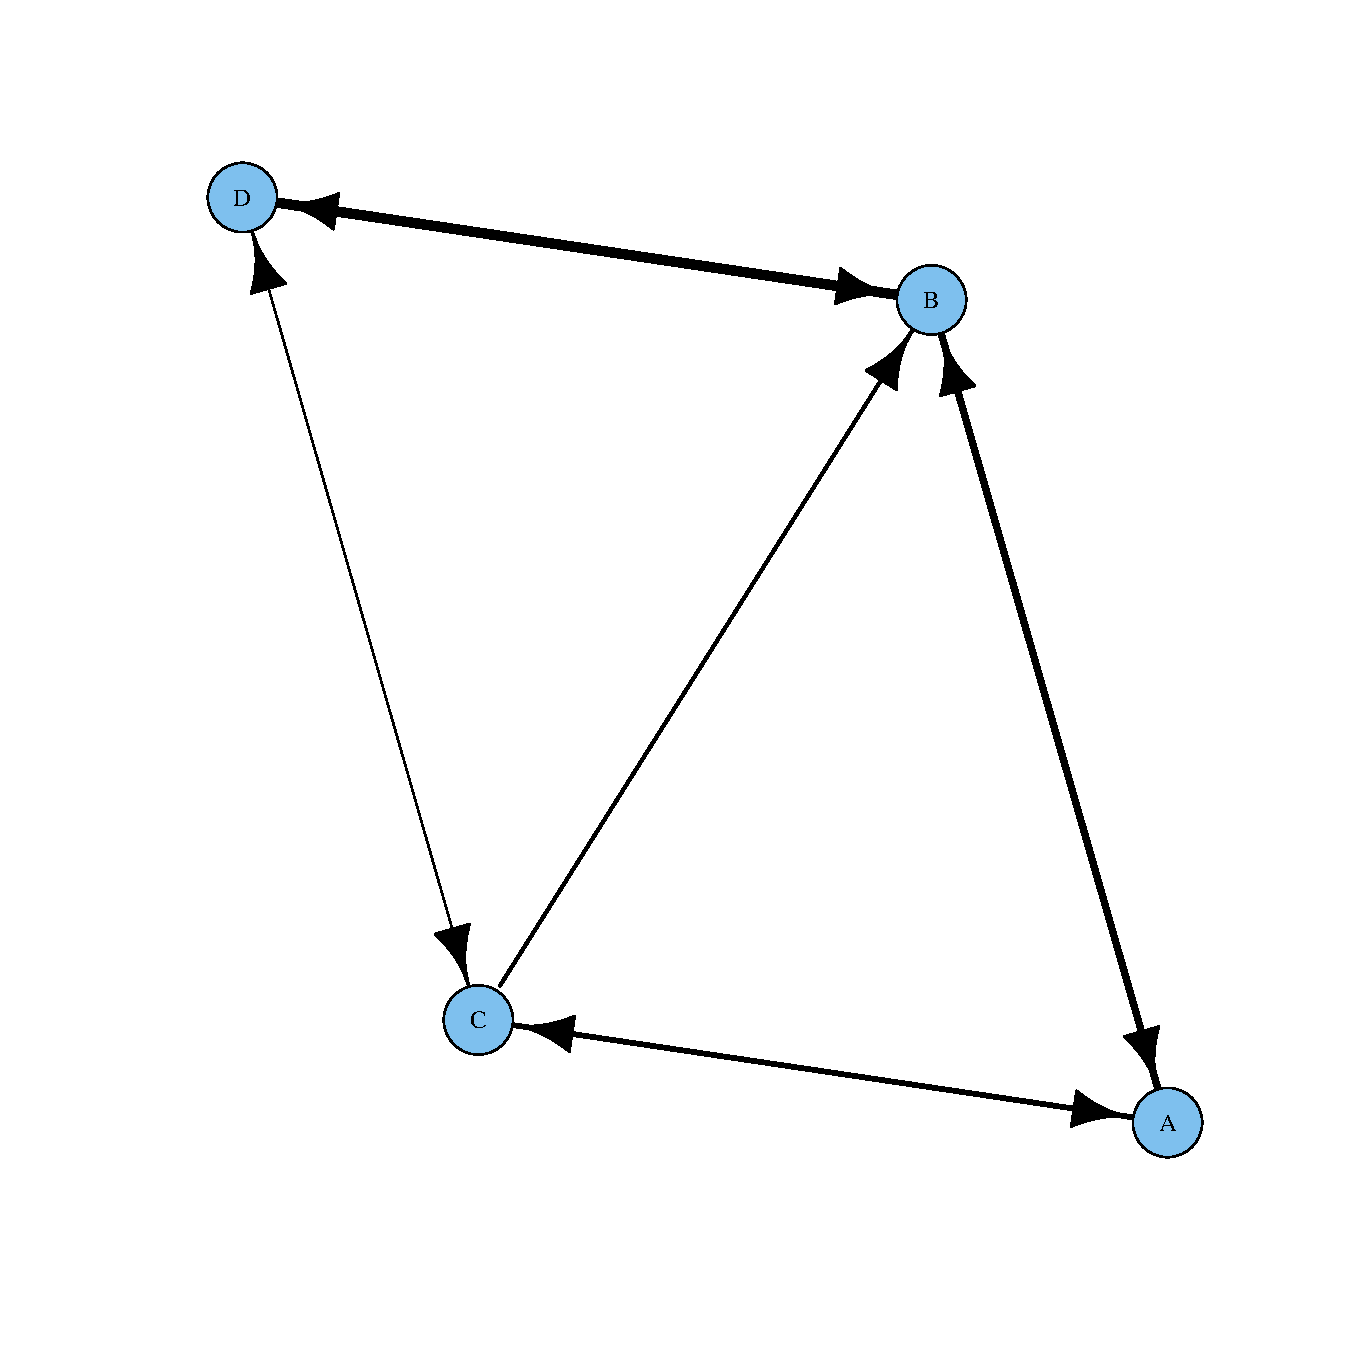
\includegraphics[width=7cm]{fig/metode/moneca_eksempel1.pdf}
}
\parbox[H]{8cm}{\null
\centering
  % \vskip-\abovecaptionskip
  \captionof{table}[t]{Adjacency matrice til netværk}%
  \vskip\abovecaptionskip
\begin{tabular}{@{}c|c|c|c|c@{}}
\multicolumn{1}{l|}{} & A & B & C & D \\ \midrule
A                     & - & - & - & - \\ \midrule
B                     & 4 & - & - & - \\ \midrule
C                     & 3 & 2 & - & - \\ \midrule
D                     & 0 & 6 & 1 & -
\end{tabular}
}
\end{figure}
%
Moneca ville i dette tilfælde komme frem til at netværket i figur \ref{monecaeksempel1} består af klyngerne [A|C] og [B|D]. Det sker ud fra følgende procedure: 
%
\begin{enumerate} \label{metode_monecastepbystep}
  \item Først lægges de to kraftigst forbundne noder sammen. Det vil her sige [B|D], hvor styrken af forbindelsen er seks.
  \item Derefter gør det den samme med de to næstmest forbundne noder, [A|B], der har en styrke på 4. Eftersom [B] allerede er en del af den foreløbige klynge [B|D], spørger Moneca om det er muligt at indlemme [A] i den allerede etablerede foreløbige klynge. Det kan ikke lade sig gøre, da [A|B] ikke er forbundne.
  \item Moneca går derfor videre til den tredje stærkeste forbindelse, [A|C]. Hverken [A] eller [C] er en del af en foreløbig klynge, og de lægges derfor sammen.
  \item Den fjerde stærkeste forbindelse er [B|C]. [B] og [C] er allerede parret med henholds [D] og [A], og Moneca beregner derfor om [A|B|C|D] udgør en klike, altså alle er forbundne med hinanden. Da det ikke er tilfældet, stopper Moneca og har dermed etableret klyngerne [A|C] og [B|D].
\end{enumerate}
% lidt usikker på om nedenstående bør tages med - det er jo beskrevet heroppe. Måske dobbeltkonfekt. 
Det vil sige at Moneca ikke etablerer nogen af de maksimale kliker, [A|B|C] eller [B|C|D]. Den semistrenge stopregel om klike-tilhørsforhold indenfor klynger betyder desuden, at man med en vis sindsro kan sige at en klynge rent faktisk \emph{er} en samlet størrelse - da den kun kan dannes hvis alle noderne har forbindelse til hinanden, hvilket eksemplet illustrerer: De to maksimale kliker etableres netop ikke, og hvis de gjorde, ville troværdigheden af grænsedragningen mellem klyngerne være langt mere tvivlsom.

For at opsummere ovenstående i mere generelle termer: Moneca starter med at slå noderne med de to mest intense forbindelser sammen til en foreløbig klynge, og går derefter videre til den næstmest intense forbindelse. Hvis en eller begge af noderne i de efterfølgende forbindelser allerede har forbindelse til en tredje eller fjerde node, vurderer Moneca, om denne indgår i en klike med den allerede etablerede klynge. Det er her vigtigt at understrege, at denne vurdering ikke er baseret på styrken af forbindelserne, men udelukkende om der eksisterer en forbindelse%
%
\footnote{Man kan forestille sig en fremtidig version af Moneca foretage en mere avanceret vurdering i disse tvivlsspørgsmål, hvori styrken af relationen kunne indgå som vurderingsgrundlag.}
%
. Moneca fortsætter med denne procedure i prioriteret rækkefølge fra de mest intense forbindelser til de mindst intense, indtil alle noder er placeret i kliker med andre noder, der endnu ikke er “optaget” af en mere intens forbindelse. Kriteriet for, om Moneca tillader at slå de tre noder sammen, er om de tilsammen former en klike, altså alle er forbundet til hinanden. Hvis de ikke er det, går den videre til den den næstmest intense forbindelse, og fortsætter med at forbinde noder indtil der ikke længere kan etableres flere kliker. Kriteriet om at allerede-etablerede klynger kun kan lægges sammen med nye noder, hvis disse indgår i en klike med alle medlemmer af klyngen, er den stop-regel, der gør at Moneca ikke bare ender med at etablere det redundante stykke information, at hvert enkelt komponent%
%
\footnote{Et komponent betyder en subgraf, hvor alle noder er forbundne gennem stier. Et netværk kan således bestå af flere komponenter, der per definition ikke er forbundne (ellers ville de være en del af samme komponent), samt noder uden forbindelse til andre noder (\emph{isolates}) \parencite[100]{Scott2000}.}% 
er en klynge i sig selv \parencite[8]{Touboel2015}. 

Efter denne  første segmentering er Moneca beregnet til at gentage proceduren indtil det ikke længere er muligt at skabe større segmenter, fordi den føromtalte klike-regel forhindrer det. Det er vigtigt at fremhæve, at Moneca i de efterfølgende klyngeinddelinger baseret den på side \pageref{monecastepbystep} beskrevne procedure, \emph{ikke} længere tager de oprindelige, interne forbindelser mellem grundkategorierne i betragtning, hvis disse er blevet lagt sammen med andre grundkategorier. I den efterfølgende klyngeinddeling vil de interne forbindelser mellem noderne på et lavere niveau ikke indgå i beregningerne i forbindelserne mellem de nyskabte noder. Det vil sige at klike-reglen kun tager højde for forbindelser til noder \emph{på det niveau noderne befinder sig på, og ikke forbindelserne på de lavere niveauer}. Når man vurderer kvaliteten af klyngerne på de højere niveauer, er det derfor centralt at se på en række standardmål for klyngens interne forbindelser, for at vurdere rimeligheden af at vurdere klyngen som en samlet størrelse. Det er dette spørgsmål vi nu afslutter gennemgangen af Moneca med.



% en lang række fordele ved at have fuld population i netværk, udover det argument vi brugte i adelsbogen, så også fx beregning af densitet (scott s. 74-5) mm. 



%%%%%%%%%%%%%%%%%%%%%%%%%%%%%%%%%%%%%%%%%%%%%%%%%%%%%%%%%%%
\subsection{Opsummering \label{}}
%%%%%%%%%%%%%%%%%%%%%%%%%%%%%%%%%%%%%%%%%%%%%%%%%%%%%%%%%%%


%%%%%%%%%%%%%%%%%%%%%%%%%%%%%%%%%%%%%%%%%%%%%%%%%%%%%%%%%%%
% Trash
%%%%%%%%%%%%%%%%%%%%%%%%%%%%%%%%%%%%%%%%%%%%%%%%%%%%%%%%%%%


%%%%%%%%%%%%%%%%%%%%%%%%%%%%%%%%%%%%%%%%%%%%%%%%%%%%%%%%%%%

%Local Variables: 
%mode: latex
%TeX-master: "report"
%End:
% 	% \input{tex/3.1_metode_arbejdsloeshed}
% 	% \input{tex/3.2_metode_netvaerksanalyse}
% 	% \input{tex/3.3_metode_disco}
% 	% \input{tex/3.4_metode_opsamling}

%%%%%%%%%%%%%%%%%%%%%%%%%%%%%%%%%%%%%%%%%%%%%%%%%%%%%%%%%%%%
\chapter{Segmenteringsprocessen og segmentkvalitet \label{desk_seg}}
%%%%%%%%%%%%%%%%%%%%%%%%%%%%%%%%%%%%%%%%%%%%%%%%%%%%%%%%%%%


dette afsnit blah blah

haha blah blah bhaha 









% 
\begin{table}[H] \centering
\caption{nøgletal for segmenteringsprocessen}
\label{4_segproces}
\resizebox{.8\textwidth}{!}{%
\begin{tabular}{@{}lrrrr@{}} \toprule										
Niveau	&	1. niveau	&	2. niveau	&	3. niveau	&	4. niveau	\\	\midrule
Antal segmenter	&	143	&	62	&	45	&	40	\\	
  Intern mobilitet i gennemsnit	&	66,9\%	&	74,5\%	&	77,2\%	&	77,6\%	\\	
  Ekstern mobilitet i gennemsnit	&	33,1\%	&	25,5\%	&	22,8\%	&	22,4\%	\\	\midrule
  Mobilitet i alt	&	100\%	&	100\%	&	100\%	&	100\%	\\	\bottomrule
\end{tabular} }
\end{table}
	%!TEX root = ../report.tex

\part{Analyse\label{part_analyse}}


%%%%%%%%%%%%%%%%%%%%%%%%%%%%%%%%%%%%%%%%%%%%%%%%%%%%%%%%%%%
\chapter{Delanalyse 1: delmarkeder og segmenter, noget i den retning \label{analyse_deskriptivt}}
%%%%%%%%%%%%%%%%%%%%%%%%%%%%%%%%%%%%%%%%%%%%%%%%%%%%%%%%%%%

Lorem ipsum dolor sit amet, consectetur adipisicing elit, sed do eiusmod
tempor incididunt ut labore et dolore magna aliqua. Ut enim ad minim veniam,
quis nostrud exercitation ullamco laboris nisi ut aliquip ex ea commodo
consequat. Duis aute irure dolor in reprehenderit in voluptate velit esse
cillum dolore eu fugiat nulla pariatur. Excepteur sint occaecat cupidatat non
proident, sunt in culpa qui officia deserunt mollit anim id est laborum.

% fra møde med Søren:
% 	Relater til forskningsspm 1, sig hvad du vil gøre (det står sort på hvidt i forskningsspm 1,)
	
% 	Opdel segprocessens 4 kort i 4 enkeltdele og smid dem ind i teksten, brug kode fra Sørens speciale. 
	
% 	skriv hvorfor det giver mening at reducere yderligere, så vi kan gå fra 274 kategorier til 51, uden at tabe intern mob, den er hele tiden sådan at "mobilitet i delmarkeder er hyppig og mellem mindre hyppig", selvom den "går lidt i stå" på de sidste 2 niveauer. Det betyder fremfor at have bygnings-arbejdere har vi en bygge-klynge. Arbejdslogik (slut evt af med det også så du kan lede det frem til delanalyse 2)

	% flere sections/sections så det ikke er så teksttungt i visse afsnit.	

	%  når der tales om et kluster skal der altid et billed med. 


%  delanalyse 2: forskelle i sociale processer: Brug løn, køn, indkomst. Bare start med den, med de lette klynger, fx fra Sørens speciale. 
% 
% 
% Sæt metodeafsnit ind uden tekst, bare "det her er og der er styr på det, du behøver ikke læse det"
% 
% 
% 





% delanalyse 3: Lav forskningsspm 3 om fra: Kan forskelle i de sociale processer vise, at der er tale om segmenter, og ikke blot delmarkeder? Hvordan kommer disse sociale processer til udtryk,  og kan moderne klassebegreber være en måde at forstå delmarkederne på som udtryk for bestemte diffentieringslogikker? Hvad siger disse diffentieringslogikker 

%  se på Goldtorpe, 
%  se på Oesh, 
%  se på Grusky
%  
% 


%%%%%%%%%%%%%%%%%%%%%%%%%%%%%%%%%%%%%%%%%%%%%%
\section{Segmenteringsprocessen \label{analyse_deskriptivt_segmenteringsproces}}
%%%%%%%%%%%%%%%%%%%%%%%%%%%%%%%%%%%%%%%%%%%%%%

De følgende netværkskort benytter den i kapitel ?? \#todo omtalte metode til at aggregere erhvervskategorier i klynger, baseret på deres mobilitetsmønstre. For at klyngerne kan siges at være egentlige delmarkeder, i Bojes definition, bør der eksistere barrierer for mobilitet mellem klyngerne. Ellers er de jo ikke til megen nytte.

Moneca var i stand til at skabe klynger frem til et 5. aggregatniveau. Tabel \ref{analyse_deskriptivt_karakteristika}  er et overblik over segmenteringsprocessen, med den gennemsnitlige interne og eksterne mobilitet i klyngerne, for hver segmenteringsniveau.

% 
\begin{table}[H] \centering
\caption{Karakteristika for segmenteringsprocessen}
\label{tab_analyse_deskriptivt_karakteristika}
\resizebox{.8\textwidth}{!}{%
\begin{tabular}{@{}l|rrrrr@{}}
Niveau	&	1. niveau	&	2. niveau	&	3. niveau	&	4. niveau	&	5. niveau	\\		\midrule
Antal segmenter	&	273	&	114	&	68	&	53	&	51	\\		
Reduktion i antal segmenter	&	-	&	139\%	&	68\%	&	28\%	&	4\%	\\		\midrule
Intern mobilitet (gns.)	&	68\%	&	75\%	&	77\%	&	78\%	&	79\%	\\		
Ekstern mobilitet (gns.)	&	32\%	&	25\%	&	23\%	&	22\%	&	21\%	\\		\midrule
Mobilitet i alt	&	100\%	&	100\%	&	100\%	&	100\%	&	100\%	\\		
Forøgelse i intern mobilitet	&	-	&	10\%	&	3\%	&	2\%	&	1\%	\\		\midrule

\end{tabular} }
\end{table}
%

Det ses at den mest markante aggregering finder sted i skiftet fra 1. niveau til 2. niveau, og herefter falder effekten af aggregeringen eksponentielt. 

På niveau går vi fra de oprindelige 273 noder til 81 klynger, bestående af 240 noder samt 33 endnu fritstående noder. Det vil sige 114 “segmenter”. Der skelnes i ovenstående tabel ikke mellem enkelte noder og klynger, da klyngernes interne mobilitet jo netop skal erstatte nodernes, og en direkte sammenligning derfor er ønskelig.
Vi ser ud fra tabellen at på 2. niveau er antallet af noder reduceret med 139 \%, og den gennemsnitlige interne mobilitet i segmenterne er steget med 7 procentpoint, svarende til en forøgelse på 10 \%. 

3. niveau inkluderer yderligere 21 enkeltstående noder i klynger, samt sammenlægger en række niveau 2 klynger. Det reducerer antallet af segmenter til 68, svarende, sjovt nok, til en reduktion på 68 \%. Det ses at stigningen i den interne mobilitet fra dette niveau og frem til niveau 5 ikke stiger væsentligt. Det lader til at en gennemsnitlig intern mobilitet tæt på 80 \% er hvad det er muligt at komme frem til. Dette forekommer rimeligt og acceptabelt, og en stigning på 11 procentpoint i den interne mobilitet fra niveau 1 til niveau 5 vurderer jeg som ganske tilfredsstillende, når det endelige resultat i gennemsnit forklarer $\nicefrac{4}{5}$ af mobiliteten. 

Fra 3. niveau og frem kan klyngedannelsen derfor primært ses som et redskab til at danne større segmenter, det vil sige reducere kompleksiteten i jobstrukturen. Det femte og endelige niveau indeholder 51 segmenter. Det betyder at den oprindelige 273 x 273 mobilitetstabel nu er reduceret til en noget mere overkommelig 51 x 51 mobilitetstabel. Ud af disse 51 kategorier er 12 enkelstående noter, der ikke er sammenlagt med andre noter, mens 39 er klynger. Medianen på det 1. niveau er på 79 \%, mens det på 5. niveau er steget til 80 \%. Standardafvigelsen for den interne mobilitet på det 1. niveau er på 12 \%, mens den på det 5. niveau er på 10 \%. Det vil sige at på de 3 centrale mål i deskriptiv statistik (Find henvisning Malchow-Muller \#todo) er mobilitetsgennemsnittene fra de oprindelige 273 mobilitetskategorier til Monecas aggregerede 51 kategorier, har der kun fundet en optimering sted: 5. niveau forklarer mere mobilitet, og kategoriernes interne mobilitet svinger mindre om gennemsnitsmobiliteten end i kategorierne på 1. niveau. Det er meget tilfredsstillende, da det indikerer at et højere aggregeringsniveau ud fra Monecas beslutningsprocedure er bedre til at forklare \emph{hvor} mobiliteten løber den, når den bevæger sig udenfor de oprindelige kategorier. Det er jo sådan set også det, den er designet til, kunne man indvende. Men det tilfredsstillende her er at helt op til \emph{det 5. aggregreringsniveau} er der stadig en bedre forklaringskraft end på de tidligere niveauer. Man kunne forestille sig at for mange kompromisser med sammenlægninger - genkald argumentet fra side ??(det om at der lægger noder sammen der rent faktisk ikke hænger sammen \#todo) ville fungere kontraproduktivt over et vist niveau, men det er altså ikke tilfældet. % ved ikke helt om det her argument egentligt holder -vil en større sammenlægning ikke bare automatisk give bedre forklaring? Nej! for hvis en node nu har meget mere udveksling med en node udenfor det, den er lagt sammen med, så ville det jo godt kunne trække ned. Men det sker ikke her, altså er det en god sammenlægning. Tror jeg. 

I figur \ref{fig_analyse_deskriptivt_kort_seg_proces} ses denne segmenteringsprocess første 4 stadier/niveauer, repræsenteret visuelt%
%
\footnote{Det 5. niveau er ikke medtaget, da det er det endelige niveau. Det vil blive præsenteret og analyseret indgående i resten af afhandlingen.}%
%
. Forskellen på hvide og sorte noder i figuren, er at hvide noder \emph{ikke} er blevet inkluderet i nogle nye klynger på det pågældende niveau. Sorte noder indikerer derimod at de \emph{er} blevet inkluderet. Så på 1. niveau er alle noderne hvide, da ingen aggregering endnu er foretaget. På niveau 2 ses det at langt de fleste noder er involveret i en aggregering, da de næsten alle er sorte. Antallet af hvide noder stiger på 3. niveau og på 4. niveau, da antallet af noder, der er muligt for algoritmen at inkludere i klynger fra det foregående niveau falder, grundet sammenlægnignskravene.   

%
%
\newgeometry{left=-0.01cm,bottom=0.1cm}
\begin{figure}[H]
\begin{center}
	\caption{Segmenteringsprocessens første 4 niveauer.}
	\label{fig_analyse_deskriptivt_kort_seg_proces}
	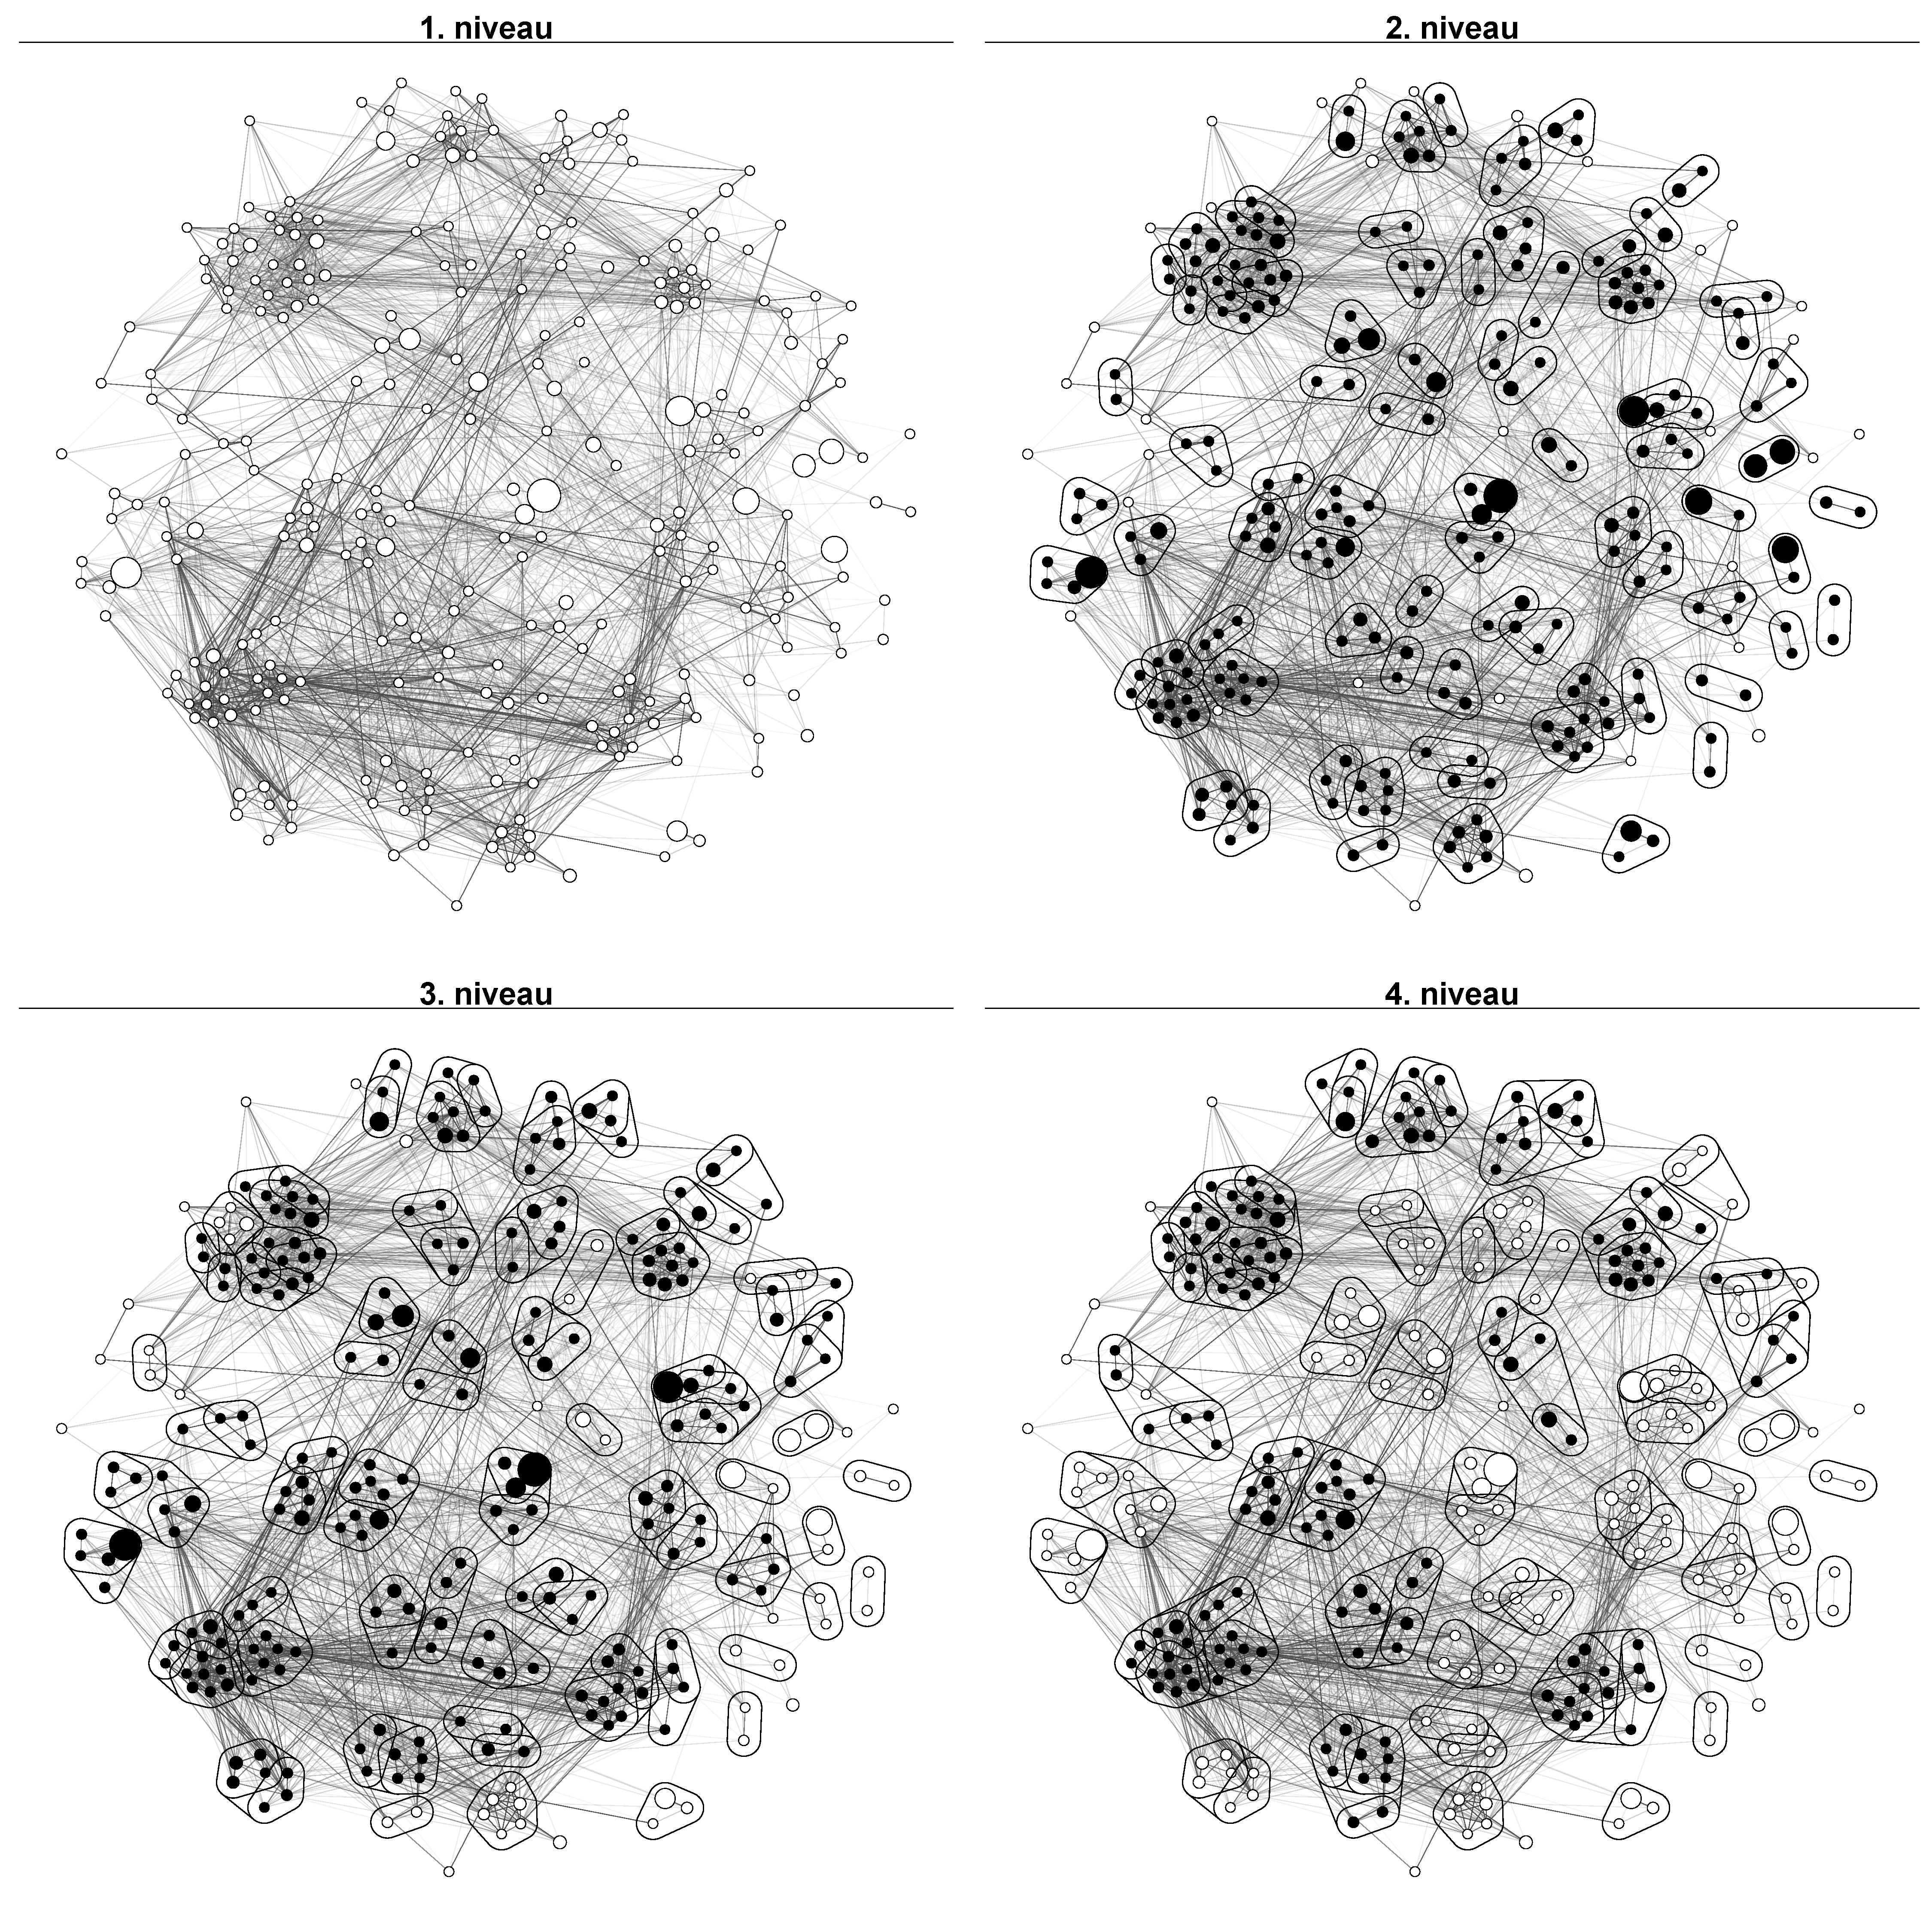
\includegraphics[width=1.0\textwidth]{fig/netvaerkskort/kort_seg_proces.pdf}
	\centerline{ \tiny{Kilde: Nielsen-Gravholt og Begtrup-Bright}}
\end{center}
\end{figure}
\restoregeometry
%
%

%%%%%%%%%%%%%%%%%%%%%%%%%%%%%%%%%%%%%%%%%%%%%%
\section{Den interne mobilitet i segmenterne \label{analyse_deskriptivt_within_mob_seg}}
%%%%%%%%%%%%%%%%%%%%%%%%%%%%%%%%%%%%%%%%%%%%%%


Det første netværkskort, jeg vil præsentere, er kortet der viser den interne mobilitet for hvert segment,  i figur \ref{fig_analyse_deskriptivt_kort_intern_mob_seg}, \pref{fig_analyse_deskriptivt_kort_intern_mob_seg}). % Den interne og eksterne mobilitet er drøftet teoretisk i afsnit ?? og den metodiske implementering er drøftet i afsnit ?? \#todo.
Da dette er det første kort, vil jeg først præsentere en vejledning i at læse de informationer, kortet indeholder. 

Noget man måske ligger mærke til ved første øjekast, er forbindelsernes farve og størrelsen af noderne. Som beskrevet i afsnit \ref{metode_relativrisiko}, er forbindelsernes styrke målt ved den relative risiko. Et forholdsmål, der udtrykker mobiliteten fra en kategori til en anden, givet den relative størrelse af antallet af beskæftigede i kategorien. Det er styrken af denne relative risiko, der afgør farven på forbindelserne: Helt lysegrå angiver en relativ risiko på 3, og helt orange angiver en relativ risiko på 15 eller derover. For at minde læseren om fortolkningen af relativ risiko (RR):  det vil sige, at der er ved en lysegrå forbindelse er 3 gange så stor sandsynlighed for mobilitet fra den forladte beskæftigelse til den nye beskæftigelse, i forhold til hvis der var tale om et helt frit arbejdsmarked. I bestemmelsen af klyngerne, er alle forbindelser med en RR på over 1 medtaget som en forbindelse. På det visuelle kort ville alle disse forbindelser ikke være til meget hjælp, da de mange pile og grå streger gør det umuligt at aflæse den underliggende systematik i hvilke forbindelser, der værd at lægge mærke til. Derfor visualiseres kun forbindelser med en RR på over 3. 

Argumentet for at vælge at sætte grænsen opadtil på 15, det vil sige reducere alle forbindelser med en RR på \emph{over} 15 \emph{til} 15 er anderledes. Her skyldes det at RR-værdierne mellem beskæftigelserne har et bredt udfaldsrum. (hvor bredt? kan du finde ud af det? \#todo) hvilket ikke er uinteressant, men repræsenteret som farvetoning på kortet, er en loyal repræsentation af denne skala ikke til meget hjælp. Visuelt er det svært at fortolke kompleksiteten, så i stedet har jeg valgt at alle RR-værdier over 15 - og der er mange - bliver sat \emph{til} 15. Derfor skal den rene orange farve tolkes ikke \emph{som} 15, men som “meget stærk” mobilitet fra en RR-værdi på 15 og op.

Størrelsen på noden repræsenterer ganske simpelt hvor mange personer, der i gennemsnit er i beskæftiget indenfor jobkategorien i årrækken 1996-2009%
%
\footnote{Når jeg fra nu af taler om hvor mange der er beskæftigede, vil det være underforstået at der er tale om det gennemsnitlige antal \emph{indenfor årrækken 1996-2009}, med mindre det eksplicit fremhæves at der er tale om noget andet.}%
%
. Ligesom med forbindelsernes styrke, er der ikke tale om et korrekt repræsenteret størrelsesforhold mellem de forskellige jobkategorier. Den største kategori, \texttt{5220: Ekspedient-, kasse- og demonstrationsarbejde} indeholder 114.869 personer i gennemsnit, svarende til 4,9 \% af det totale antal beskæftigede. Mens den mindste, \texttt{7346: Serigrafisk arbejde} indeholder 504 personer, svarende til 0,02 \% af det totalen. Det er for komplekst til visuel afkodning i et allerede informationstungt netværkskort, da de mindste noder ville blive meget små og de store noder voldsomt store. Derfor har jeg valgt et størrelsesforhold mellem noderne, der ikke er 1:1 med deres reelle forskelle i størrelse, men som alligevel giver en fornuftig fornemmelse for de reelle størrelsesforhold.  

Man skal dermed se både farve af forbindelserne og nodernes størrelse som en grov målestok af den variabel, den repræsenterer. Med vægten lagt på nem visuel afkodning, fremfor korrekt gengivelse af dataens reelle kompleksitet. Forbindelsernes styrke og beskæftigelseskategoriernes størrelse vil blive gennemgået nærmere senere, her præsenteres de kun med det formål at kunne aflæse kortene.  

Til sidst skal læseren mindes om, at der er tale om et retningsbestemt netværk, hvor pilene på kortet angiver retningen af mobiliteten mellem noderne. 

Det var de generelle retningslinjer for kortene. Dette gælder alle de præsenterede kort. Næste side indeholder(??) det første kort, der er farvelagt efter den interne mobilitet på segmentniveau.


\newgeometry{left=-0.01cm,bottom=0.1cm}
\begin{figure}[H]
\begin{center}
	\caption{Intern mobilitet for segmenterne.}
	\label{fig_analyse_deskriptivt_kort_intern_mob_seg}
	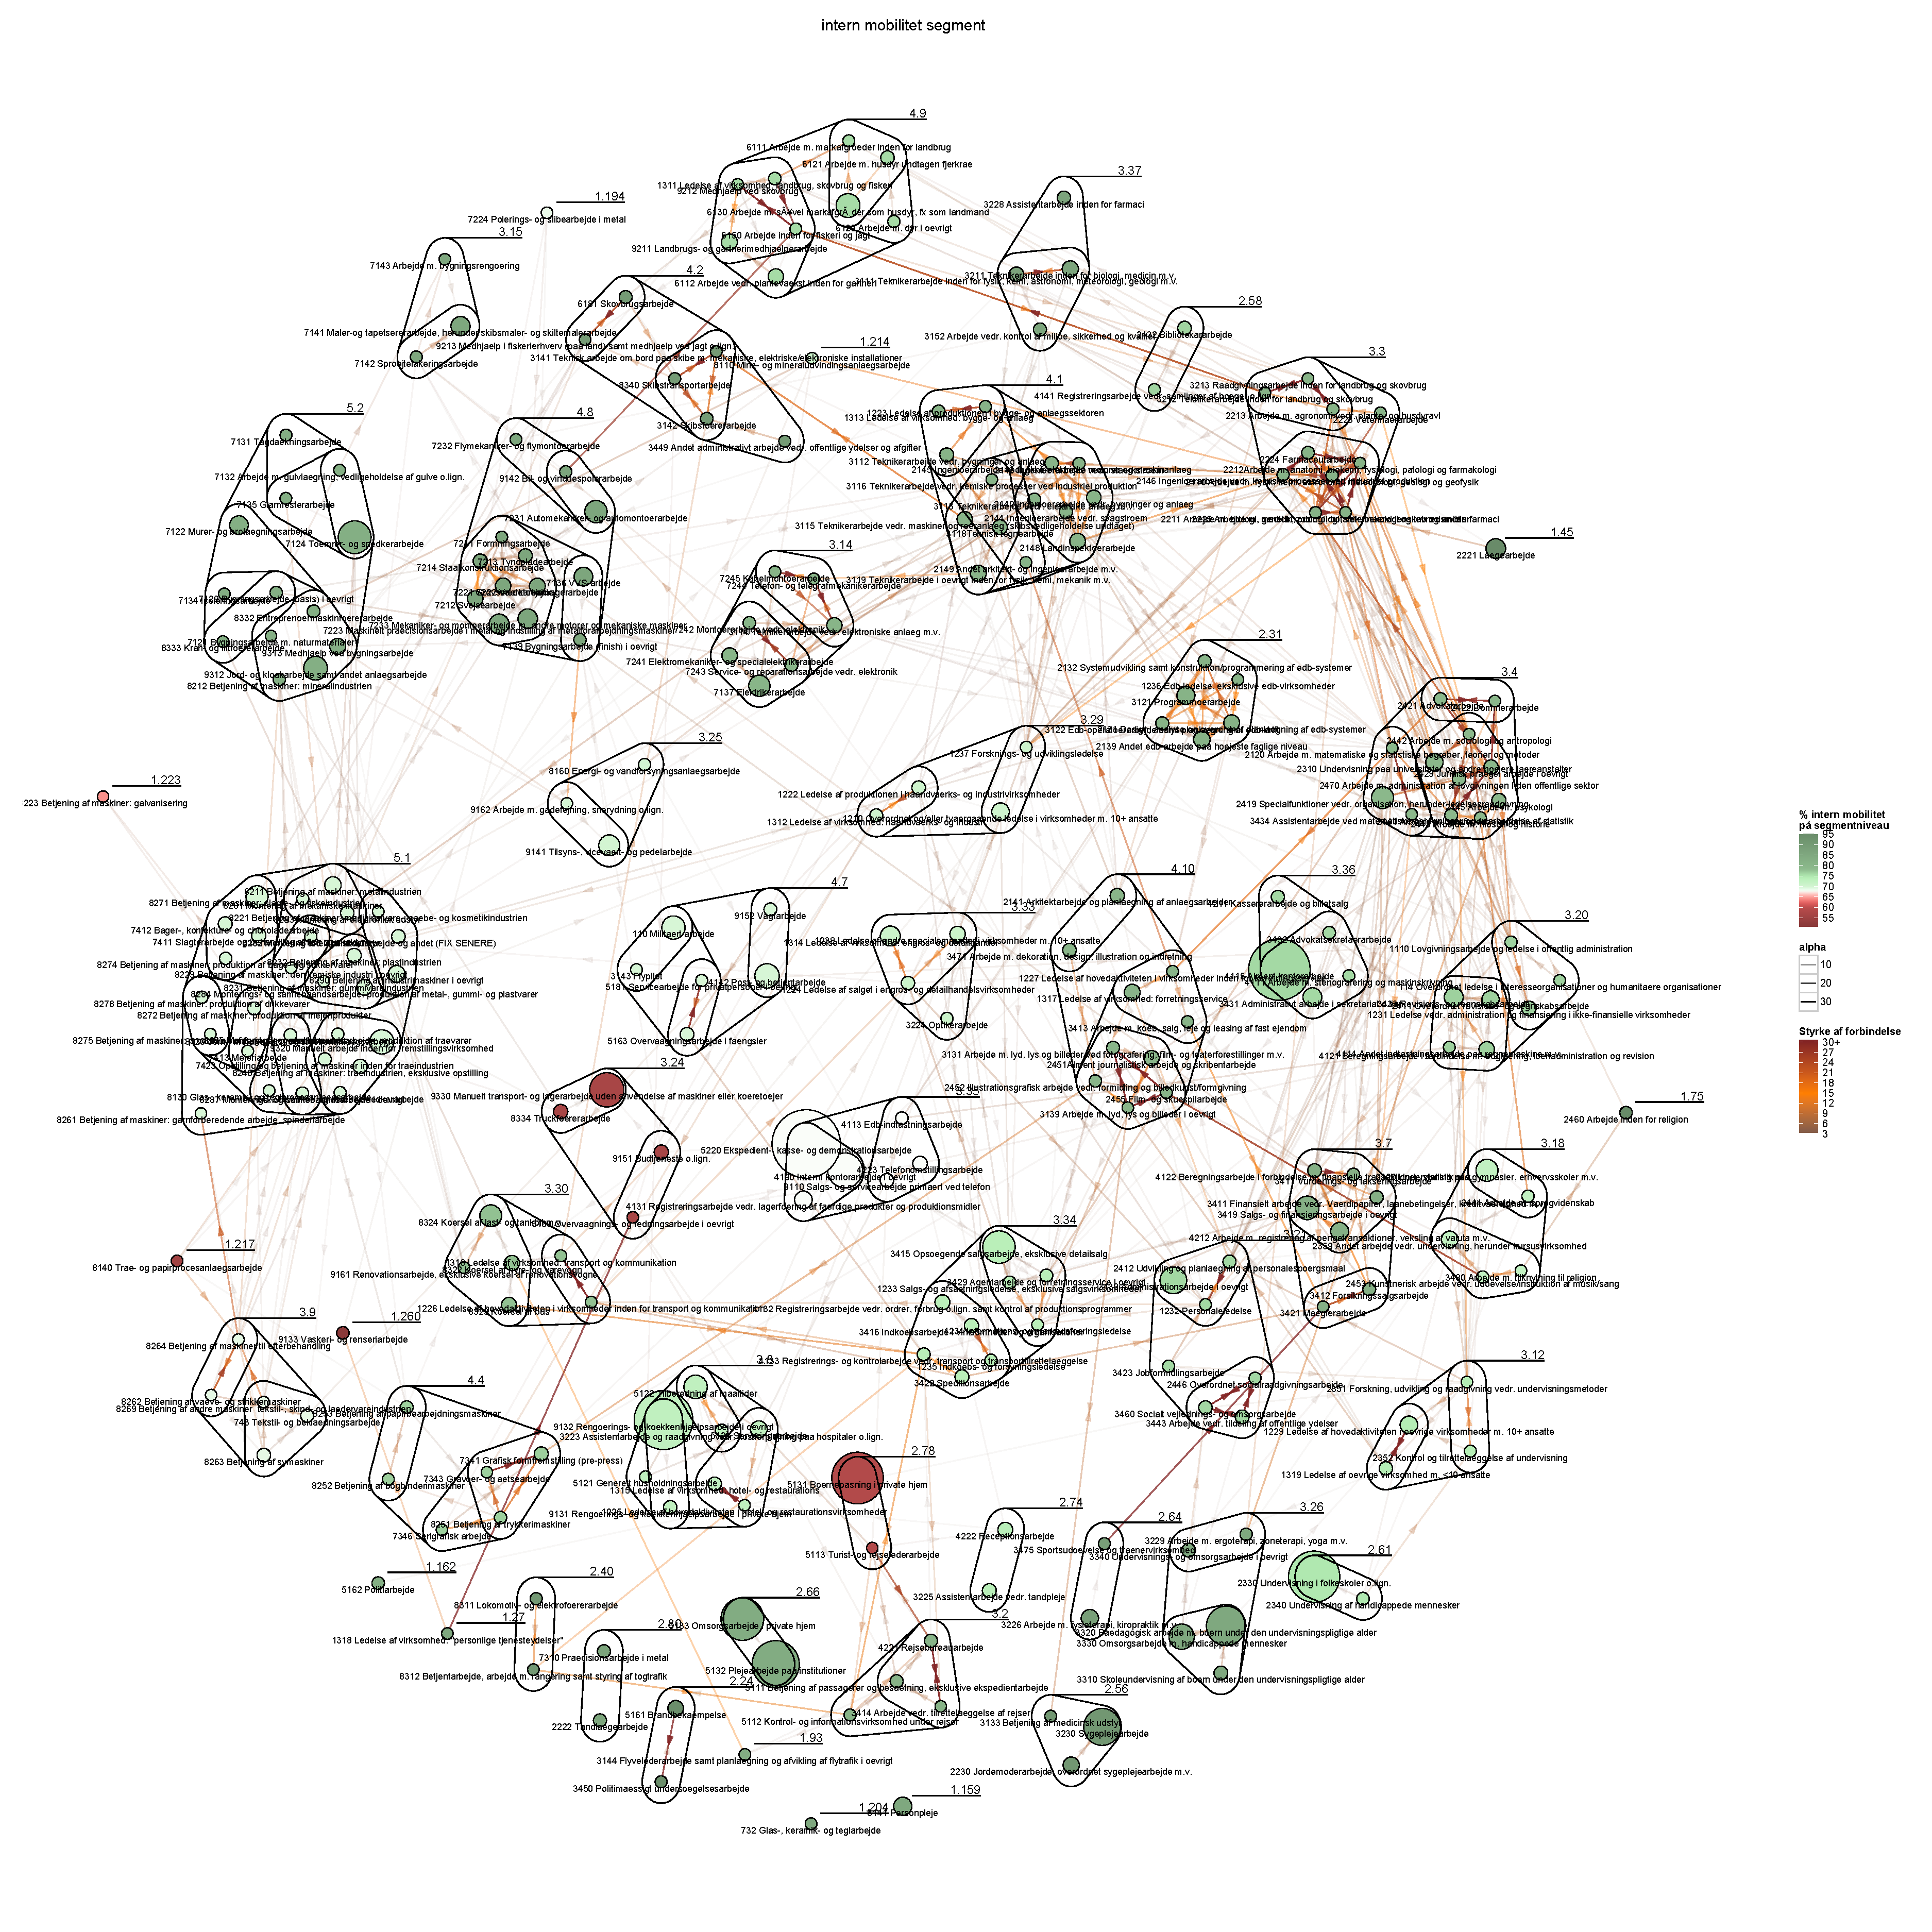
\includegraphics[width=1.0\textwidth]{fig/netvaerkskort/kort_intern_mob_seg.pdf}
	\centerline{ \tiny{Kilde: Nielsen-Gravholt og Begtrup-Bright}}
\end{center}
\end{figure}
\restoregeometry

Det ses på kortet, at nodernes farve går fra mørkerød, til hvid, til mørkegrøn. Mørkerød betyder at klyngen har en intern mobilitet på mellem 50 og 60 \%, mens den derfra og op til 69 \% antager en stadigt svagere lys rød, indtil den er ren hvid ved 70 \%. Derfra og op til 78 \% bliver den stadig mere grøn, for ved 80 \% at være helt mørkegrøn. Da der er tale om en gradient, er skiftet i farve ikke diskret, men kontinuert. 

Skiftet i farve er motiveret af min egen vurdering. Der findes ingen tidligere brug af Moneca algoritmen, hvori dette indgående bliver analyseret. Jeg har derfor besluttet mig for, at en mobilitet mellem erhvervene i en klynge på 70 \% og derover, er en fornuftig tærskel at benytte til at  vurdere kvaliteten af et segment, på dette parameter. Det ses at langt de fleste klynger overholder denne beslutningsregel. Klynge \emak{s5.1} har en intern mobilitet på 69,4 \%. Jeg vil betragte det som acceptabelt, da det ligger så tæt på min tærskelværdi. Der er ikke er tale om en statistisk test med et vist signifikansniveau, men min egen tentative vurdering. Og selv med de vedtagne signifikansniveauer i statistiske test, eksempelvis p-værdier i en T-test eller en F-test,  der advarer litteraturen om ikke at tolke disse tærskelværdier som skrevet i sten, men som nyttige konventioner (find henvisning, Gujarati og Malchow-Møller \#todo). 

Der kan være to årsager til lav intern mobilitet. Den ene er at beskæftigelserne i disse klynger simpelthen er jobs, der af den ene eller anden årsag er af en type, hvor folk sjældent opholder sig længe i dem. Det kunne være ufaglærte jobs, der typisk henvender sig til unge og studerende. Eller ufaglært, sæsonbetinget arbejde, eller jobs der simpelthen er så hårde, eller ansættelserne så usikre, at man ikke bliver i dem længe af gangen. Hvis arbejdet har denne karakter, må man forvente, at de sociale lukningsmekanismer næppe er særlig højtudviklede, hvoraf den mest legitime i moderne samfund må være adgangsgivende uddannelse. Vi vil derfor forvente at finde enten ufaglærte eller fag med lave uddannelsesmæssige krav. 

Hvis vi kigger på klynge \emak{s2.78}, kan vi se at den består børnepasning i private hjem, samt turist- og rejseledere, der har en intern mobilitet på henholdsvis  59 \% og 47 \%, altså ganske lavt sammenlignet med den gennemsnitlige interne mobilitet indenfor erhvervene selv, der er på 68 \%.  Begge jobs er indenfor hovedgruppe 5 i Disco-nomenklaturet, salgs-, service- og omsorgsarbejde. Det er arbejde, der ifølge Danmarks Statistik er klassificeret som ISCEDs færdighedsniveau 2, hvilket betyder at det kræver uddannelse “på grundniveau” \parencite[tabel 1]{DSTDISCO88}. Det er en klar indikator på at de formelle sociale lukningsmekanismer i erhvervene er begrænsede. 


Der er imidlertidig også andre klynger på kortet, hvor uddannelseskravene er lave, men hvor den interne mobilitet er høj. Et nærliggende eksempel er klynge \emak{s2.66}, Der ligeledes befinder sig i hovedgruppe 5, men hvor den interne mobilitet både i klyngen og blandt jobbene selv er meget høj. Børnepasning i private hjem ligger ganske tæt på arbejdsfunktionerne i klynge \emak{s2.66}, faktisk så tæt at de også på et 3-cifret Disco niveau er kategoriseret ens. Men børnepasning i private hjem har tilsyneladende en noget anden social profil. Den interne mobilitet er meget lavere, og den ligger sammen med turist- og rejseleder. 

Det ses også at der ikke er nævneværdig mobilitet mellem de to klynger, trods denne enshed. Det får mig til at konkludere, at der trods en vis funktionel enshed mellem børnepasning på en ene side og omsorgsarbejde for ældre mennesker i deres hjem og på institutioner på den anden, er tale om vidt forskellige sociale processser. Den funktionelle enshed er ikke bestemmende for den sociale ditto. Det viser sig også ved at gennemsnitlige alder indenfor klynge \emak{s2.78} er omtrent 37 år.%
%
\footnote{Det også gælder de to jobs i klyngen hver især}%
%
. Klynge \emak{s2.66} har en gennemsnitsalder på 42 $\nicefrac{3}{4}$ år, hvilket er er nærmest identisk med populationsgennemsnitet på 42,3 år. (check hvilken kvartil det befinder sig i på forskermaskinen \#todo). 


















%%%%%%%%%%%%%%%%%%%% noter %%%%%%%%%%%%%%%%%%%%%%%%%%%%%%%%%%%%%%%%%%%


%  Måske skal der laves mere stringent begrebsafklaring om forskel på delmarkeder, segmenter og klynger. 




% \input{tex/5.0_diskussion}

% \input{tex/6.0_konklusion}





% %%% -------------- Appendiks ----------------- %%%
%i en tidligere version hed det appendices i stedet for appendix, så hvis appendikset ikke dukker frem så prøv i stedet
%\begin{appendix}

%\setcounter{secnumdepth}{3}
% % \input{tex/app_figurer}
% %!TEX root = ../report.tex

%%%%%%%%%%%%%%%%%%%%%%%%%%%%%%%%%%%%%%%%%%%%%%%%%%%%%%%%%%%
\newpage \chapter{variabelbeskrivelser: løn \label{app_loen}}
%%%%%%%%%%%%%%%%%%%%%%%%%%%%%%%%%%%%%%%%%%%%%%%%%%%%%%%%%%%

Jeg har valgt at beskrive indkomstbeskrivelse i realindkomst, da denne gør det muligt at lave sammenligninger i indkomst over tid. Alternativet er en nominel indkomstbeskrivelse, altså blot kroner og ører, som det ser ud på et givent tidspunkt \parencite[6]{DST2009}. 
En beskrivelse af realindkomsten tager udgangspunkt i købekraften, som den reelt ser ud, og korrigerer således for inflation mv. Tallene korrigeres ud fra forbrugerprisindekset \parencite{DSTPRISINDEKS}. 

Monecakortet er, som beskrevet i ???, et tværsnit lavet på baggrund af 1996 til 2009, altså 14 år. Et lignende tværsnit af indkomst virker derfor mest fornuftigt, da det på samme måde som selve netværkskortet viser strukturen, som den ser ud gennem alle de 14 år. Et alternativ ville være at vise lønninger for et enkelt år, eksempelvis det seneste, 2009. Det mener jeg ville være misvisende, da det ikke tager højde for de strukturelle udsving i indkomsten, der uværgeligt forekommer over en periode på 14 år. Derfor forekommer et gennemsnit af indkomsten over de 14 år som den fornuftigste måde at beskrive indkomst på, indenfor denne afhandlings rammer. Metoden til det er som nævnt at korrigere hvert af de tidligere år, således at alle indkomster i årene 1996-2008 bliver opdateres til 2009-priser, hvorefter gennemsnittet tages. 

Danmarks Statistik har en række indkomstvariable til rådighed. Disse variable registrerer indkomst ud fra en række forskellige parametre. Selv tilsyneladende ens variable har alligevel diskrete, omend ofte betydningsfulde, forskelle i opgørelsesmetoden. Dette er ikke uskyldige forskelle, og i sammenligning af variablenes centralmål er det tydeligt, at disse forskellige opgørelsesmetoder har stor betydning for variablenes fordelinger.

Eksempelvis registrerer \texttt{DISPO\_NY} den disponible indkomst efter skat og renter, mens \texttt{perindkialt} registrerer personindkomst i alt, hvilket defineres som summen af erhvervsindkomst, overførselsindkomst, formueindkomster samt anden ikke-klassificerbar indkomst, altså hvad der forekommer som rub og stub. Disse to variable beskrivelser et individs samlede indkomst, men på forskellige måder, hvoraf den mest centrale og iøjnefaldene er, at den sidstnævnte måler før skat, og førstnævnte er efter skat. Derudover registreres den samlede indkomst ud fra forskellige kilder, som ikke altid er lige lette at gennemskue betydningen af. Dette ses også i deres fordelinger, samt i mængden af fejlværdier såsom negative indkomstværdier m.m.

Andre variable registrerer løn direkte, såsom \texttt{loen\_mv}, der inkluderer hele den skattepligtige lønindkomst, inklusiv frynsegoder, skattefri løn, jubilæums- og fratrædelsesgodtgørelser samt værdi af aktieoptioner. Det gælder også \texttt{jobloen}, hvis opgørelsesmetode i beskrivelsen hos DST er mere centreret på ansættelses i registreringsmåneden november, omend også inkluderer andre ansættelser i ikke-novemberansættelser, som de kalder det. \label{indkomstvariable}

Det har vist sig, at stort set alle indkomstvariablene, som jeg har til rådighed i registerdataet, ligger en del lavere end de tal, DST selv benytter til at beskrive løn indenfor forskellige \texttt{DISCO}kategorier i deres rapport \emph{Indkomst} fra 2009  \textcite{DST2009}.  

Den eneste variabel, hvor det ikke er tilfældet, \texttt{TIMELON}, der beskriver timelønnen. Det er den variabel, der, udover sin kvalitet i form af let fortolkbarhed, kommer tættest DSTs egne tal i rapporten \emph{Befolkningens løn} fra 2012. Denne variabel vil derfor benyttes til at beskrive lønindkomst i denne afhandling, og selvom nedenstående vil inddrage de andre indkomstvariable som reference, er denne variabel, dens validitet og central omdrejningspunktet for dette appendiks. 

\section{Timeløn \label{}}

variablen \texttt{TIMELON} har til formål at beskrive timelønnen, også for danskere, hvori lønninger normalt ikke opgøres i timeløn. “Variablen angiver den gennemsnitlige timeløn i novemberansættelsen for hoved- og bibeskæftigede lønmodtagere.” \parencite{DST-TIMELON}. Lønnen, der indgår i den gennemsnitlige timeløn, er det beløb, der årligt indberettes af arbejdsgiveren på oplysningssedlen til Skat. Dvs. at der indgår løn, feriegodtgørelse, løn under sygdom mv. Bidrag til pensionsordninger medregnes ikke. 

Den centrale vanskelighed ved at beskrive timeløn, er, iflg. DST, at bestemme antallet af arbejdstimer for den enkelte, således at timelønsskønnet er pålideligt. Til at bestemme kvaliteten af timelønsskønnet i \texttt{TIMELON}, findes variablen \texttt{TLONKVAL}, der går fra 0 \% til 100 \%, hvor 0 \% er maksimal sikkerhed af skønnet, og 100 \% er maksimal usikkerhed. I denne vurdering indgår en række elementer til bestemmelsen af antal arbejdstimer, trukket af arbejdsgiverens oplysningssedler, ATP-biddrag mm. DST skriver, at værdier fra 0 til 50 \% er af brugbar kvalitet, mens >50 \% er af tvivlsom kvalitet. DST skriver om kvaliteten, at “\emph{Set for alle ansættelsesforhold under ét er der en rimelig overensstemmelse mellem den beregnede timeløn i IDA og Danmarks Statistiks lønstatistik. For ansatte på fuld tid er der for 44 pct. af lønmodtagerne en forskel på 5 kr. eller mindre (Det økonomiske Råds sekretariat 2003). Der kendes ingen kvalitetsundersøgelser på et mere detaljeret niveau. }” \parencite{DST-TIMELON}. Det centrale her er, at der ingen kvalitetsundersøgelser findes på et mere detaljeret niveau. 

Der er derfor to problemer på spil i ovenstående: \emph{Det første} er, at \texttt{TIMELON} beregnes for novemberansættelsen et givent år, hvorimod vores \texttt{DISCO}-variabel benytter den længste ansættelse indenfor et givent år. Der er, for mange mennesker, med ganske stor sandsynlighed fin overenstemmelse mellem længste ansættelse, og novemberansættelsen. Men vi har ingen mulighed for at tjekke det. \emph{Det andet problem} er det, DST skriver i ovenstående paragraf: Der findes ingen kvalitetsundersøgelse af \texttt{TIMELON} på et mere detaljeret niveau. Et sådant detaljeret niveau kunne eksempelvis være inddelingen af befolkningen i 150 arbejdskategorier. Som jeg gør det, i dette speciale. 

For at komme det første problem til livs, vælger jeg derfor at fjerne alle observationer med en \texttt{TLONKVAL} på >50 \%. Det sker naturligvis ud fra DSTs anbefaling om at disse er “af tvivlsom kvalitet” generelt, men især fordi, at dette mål for tvivlsom kvalitet er baseret på deltidsansættelse. Det er mit skøn, at ved at fjerne personer, der arbejder under halv tid på et år, fjerner jeg mange af de fejl, der måtte forekomme, hvis en person, der 3 måneder af året arbejder som taxachauffør, men tilfældigvis i november har en ansættelse som jord- og betonarbejder. Det ville betyde, at jeg i min benyttelse af \texttt{TIMELON} ville få registreret lønnen som taxachauffør som en jord-og betonarbejder lønning. Ved at fjerne dem, hvor deres \texttt{TIMELON} ansættelse er under halvdelen af året, er faren for fejlkategoriserede lønninger reduceret væsentligt, da jeg nu kun har lønninger med for folk, der arbejder over halvdelen af året. Chancen for at denne halvdel af året inkluderer november, er derfor over halvdelen. Dette er naturligvis ikke en skudsikker gardering overhovedet, men er en nem måde at fjerne, så vidt jeg kan vurdere, den værste kilde til fejl i min lønbeskrivelse.

min bedste mulighed for at vurdere omfanget af disse problemer for validiteten af \texttt{TIMELON}, er i sidste ende at undersøge dens overenstemmigelse med virkelighedens lønninger. Den overenstemmigelse har jeg mulighed for at vurdere via følgende 3 metoder:

\begin{enumerate}
  \item DSTs timelønsbeskrivelser i rapporten \emph{Befolkningens Løn 2012}
  \item common sense vurdering af lønniveauer for forskellige genkendelige faggrupper
  \item Den relationelle forskel mellem de forskellige lønninger, og hvorvidt denne relationelle forskel er konsistent med de relationelle forskel jeg ser i andre af DSTS indkomstvariable
\end{enumerate}


\section{Centrale mål \label{}}

Nedenstående tabel \ref{app_timelon1996_2009} viser de centrale mål for hvert år af \texttt{TIMELON}. Disse er ikke korrigeret for inflation, da jeg har valgt ikke at omregne hele populations individuelle lønninger med forbrugerprisindekset, og i stedet kun valgt de relevante gennemsnitsværdier. Standardafvigelse og percentiler kan naturligvis ikke vises medmindre hele populations observationer er i samme enhed, derfor denne fremstillingsform. 

Det bemærkes at ingen har en timeløn under 11 kr. Det skyldes at jeg har fjernet alle observationer der tjener mellem 0 og 10 kr, da dette forekom som en kunstigt lav timeløn, der kun kunne forekomme, grundet udregningsmetoden i \texttt{TIMELON}-variablen. Dette ville, ifølge mit skøn, give et misvisende billede af den reelle timeløn indenfor en given disco-kategori. I gennemsnit fjernes 369 personer pr. år på denne måde, altså et ubetydeligt bortfald. 

Det ses desuden i tabel \ref{app_timelon1996_2009} der i 2003 sker et lille fald i gennemsnitslønnen, fra 185,5 kr/t til 184,8 kr/t. Det efterfølgende år sker der en relativt kraftig stigning til 195,2 kr/t. Dette skyldes databrud hos DST. I denne henseende er det en fordel at min datastruktur kræver et gennemsnit over den 14-årige periode, da et databrud i en kortere periode indenfor tidsrammen derfor er af mindre betydning. 

\begin{table}[H] \centering
\caption{centrale mål for TIMELON, 1996-2009}
\label{app_timelon1996_2009}
\resizebox{1.0\textwidth}{!}{
\begin{tabular}{@{}lrrrrrrrrrrrrrr@{}} \toprule	
År	&	1996	&	1997	&	1998	&	1999	&	2000	&	2001	&	2002	&	2003	&	2004	&	2005	&	2006	&	2007	&	2008	&	2009	\\	\midrule
N	&	1677704	&	1738875	&	1755089	&	1789319	&	1624672	&	1638380	&	1582448	&	1508256	&	1512068	&	1530139	&	1526006	&	1587350	&	1521759	&	1647924	\\	
Gennemsnit (2012 priser)	&	211,6	&	208,5	&	216,1	&	215,5	&	217,5	&	223,5	&	221,8	&	223,5	&	219,8	&	227,8	&	232,0	&	234,9	&	236,90	&	239,35	\\	
Gennemsnit (2009-priser)	&	196,8	&	193,9	&	201,0	&	200,4	&	202,2	&	207,8	&	206,3	&	207,9	&	204,4	&	211,9	&	215,7	&	218,4	&	220,31	&	222,58	\\	
Gennemsnit	&	150,6	&	151,6	&	159,8	&	163,9	&	169,8	&	177,7	&	181,3	&	185,6	&	184,8	&	195,2	&	202,3	&	209,8	&	217,4	&	222,6	\\	
Sdafvigelse	&	67	&	66	&	72	&	74	&	78	&	83	&	84	&	84	&	84	&	90	&	99	&	102	&	113	&	108	\\	
Mindste værdi	&	11	&	11	&	11	&	11	&	11	&	11	&	11	&	11	&	11	&	11	&	11	&	11	&	11	&	11	\\	
Højeste værdi	&	9974	&	5970	&	5952	&	8772	&	8019	&	9826	&	6850	&	7158	&	15165	&	8323	&	29429	&	11940	&	16977	&	28752	\\	
p25	&	115	&	116	&	121	&	125	&	129	&	135	&	137	&	141	&	141	&	149	&	154	&	159	&	164	&	169	\\	
p50	&	139	&	140	&	147	&	151	&	156	&	163	&	167	&	171	&	170	&	180	&	187	&	194	&	200	&	204	\\	
p75	&	170	&	171	&	181	&	185	&	192	&	201	&	205	&	210	&	208	&	220	&	228	&	237	&	245	&	250	\\	
p90	&	218	&	218	&	232	&	237	&	245	&	257	&	262	&	267	&	265	&	279	&	289	&	300	&	312	&	318	\\	
p99	&	379	&	380	&	408	&	418	&	433	&	456	&	467	&	476	&	477	&	499	&	521	&	548	&	580	&	580	\\	\bottomrule
\end{tabular} }
\end{table}

Jeg har benyttet forbrugerindekset til to korrektioner af lønningerne. omregningen til 2012 priser sker for at kunne sammenligne direkte med DSTs rapport fra 2012, og omregningen til 2009 priser bliver benyttet i afhandlingen. Det kan måske forekomme omstændigt, men det virker mest hensigtsmæssigt at benytte et prisniveau fra et år i den tidsperiode, der rent faktisk er i analysen, fremfor et prisniveau 3 år længere fremme i tiden, og som udelukkende er med for at kunne teste validiteten af variablen op imod DSTs rapport.

\begin{table}[H] \centering
\caption{centrale mål for TIMELON, 1996-2009}
\label{app_timeloninf}
\begin{tabular}{@{}lccc@{}} \toprule								
	&	2009 priser	&	2012 priser	&	DST 2012	\\	\midrule
gennemsnitsløn	&	207,8	&	223,5	&	243,0	\\	
N	&	\multicolumn{2}{c}{1.617.142}			&	1.353.000	\\	\bottomrule
\end{tabular}
\end{table}

% \begin{table}[]
% \centering
% \caption{My caption}
% \label{my-label}
% \begin{tabular}{cccc}
% 					& 2009      & 20012     & dst \\
% A                    & -         & -         & -   \\
% n                    & \multicolumn{2}{c}{4} & -  
% \end{tabular}
% \end{table}




Det ses af tabel \ref{app_timeloninf}, at den gennemsnitlige timeløn i perioden 1996-2009, omregnet til 2012-priser, er 223,5 kr/t. i DST rapporten omhandlende samme år, er de kommet frem til en gennnemsnitsløn på 243 kr/t, altså en forskel på 19,5 kr i timen. Det er naturligvis en klar forskel. Det er dog ikke så bekymrende, når man medtager det forhold, at der faktisk ikke er tale om to direkte sammenlignende tal: DSTs gennemsnitslønning er et forsøg på at ramme den reelle gennemsnitsløn for et bestemt år, her 2012. Mit formål er imidlertidig at beskrive lønniveauet i en 14-årig periode. Det betyder at min gennemsnitslønning også indeholder strukturelle forskydninger og konjunktursvingninger i økonomien, som den har  udviklet sig over de 14 år. Det er derfor forventeligt, at den ikke rammer præcis gennemsnitslønnen, som den så ud i et enkelt år, her 2012. I denne optik er forskellen på 19,5 kr på ingen måde bekymrende. Det ses også, at mit N har 264.142 flere personer i gennemsnit over årene, end DST benyttede til deres rapport i 2012. Datarensningen i DSTs rapport fremgår ikke tydeligt, så det er ikke muligt at klargøre hvorfor denne forskel eksisterer. Det er dog ikke bekymrende, når gennemsnittet alligevel ligger acceptabelt tæt.  



\section{sammenligning med DSTs rapport \label{app_indkdstrapport}}

Grundet omkodninger og xx (det ord Søren bruger) fra et 4-cifret DISCO-niveau til mit, omtalt i Bilag (\#henvisning), er det ikke muligt at sammenligne direkte med DSTs rapport om timelønninger fra forskellige faggrupper. I 19 tilfælde svarer mit DISCO-variabel imidlertidig direkte til DSTs oprindelige 4-cifrede niveau. Det er således muligt at lave en sammenligning mellem mit data og DSTs timelønsrapport, for at få en indikator på validiteten af mine timelønninger. Disse 19 tilfælde er opgjort i Tabel \ref{app_timelon_dstsammenligning}. Det viser timelønnen i mit data, i DST rapporten, forskellen i timellen opgjort i absolutte værdier samt i procent. Rangeringen går fra højeste positive forskel til mellem DST rapportens timeløn for faggruppen og min timeløn for faggruppen, til højest negative forskel ditto. Det vil sige at at en positiv forskel i timeløn, rangeret øverst, betyder at mine tal ligger \emph{under} x antal kroner under DSTs timelønssats, og en negativ forskel i timeløn, rangeret lavest, betyder at min timelønssats ligger x antal kroner \emph{over} DSTs timelønssats. Endelig er den gennemsnitlige (numeriske) forskel opgjort nederst, i absolut værdi og i procent. Min timelønssats er som omtalt korrigeret til 2012-priser. 

\begin{table}[H] \centering
\caption{Sammenligning med DST rapport}
\label{app_timelon_dstsammenligning}
\resizebox{1.0\textwidth}{!}{
\begin{tabular}{@{}lrrrrr@{}} \toprule
Discokode	&	Eget data, sdafvigelse 2009	&	Eget data, gns.	&	DST rapport, gns.	&	Forskel	&	Forskel i procent	\\	\midrule
110: Militaert arbejde	&	78	&	218	&	312	&	94	&	29 \%	\\	
7139: Bygningsarbejde (finish) Elektriker	&	75	&	192	&	220	&	28	&	12 \%	\\	
3111: Teknikerarbejde inden for fysik, kemi, astronomi, \\ meteorologi, geologi mv	&	55	&	193	&	219	&	26	&	11 \%	\\	
7124: Bygningsarbejde (basis), toemrer- og snedkerarbejde	&	64	&	186	&	205	&	19	&	9 \%	\\	
4110: Alment kontorarbejde	&	60	&	182	&	199	&	17	&	8 \%	\\	
3118: Teknisk tegnearbejde	&	48	&	200	&	214	&	14	&	6 \%	\\	
7122: Bygningsarbejde (basis), murer- og brolaegningsarbejde	&	65	&	197	&	210	&	13	&	6 \%	\\	
3112: Teknikerarbejde vedr. bygninger og anlaeg	&	72	&	246	&	259	&	12	&	4 \%	\\	
2141: Ingenioerer og arkitekter	&	108	&	306	&	317	&	11	&	3 \%	\\	
2221: Laege	&	155	&	391	&	401	&	10	&	2 \%	\\	
2411: Overordnet revisions- og regnskabsarbejde, herunder \\ registeret revisor og statsautoriseret revisor	&	172	&	300	&	308	&	8	&	2 \%	\\	
2331: Folkeskolelaerer	&	49	&	219	&	224	&	5	&	2 \%	\\	
9130: Rengoerings- og koekkenhjaelpsarbejde	&	48	&	158	&	162	&	4	&	2 \%	\\	
3113: Teknikerarbejde vedr. elektriske anlaeg mv	&	72	&	266	&	267	&	1	&	0 \%	\\	
3114: Teknikerarbejde vedr. elektroniske anlaeg mv	&	77	&	257	&	251	&	-6	&	-2 \%	\\	
3115: Teknikerarbejde vedr. maskiner og roeranlaeg, eksklusiv \\ vedligeholdelse af maskiner om bord paa skibe	&	74	&	265	&	250	&	-14	&	-5 \%	\\	
8322: Koersel af hyre- og varevogn m.v. 	&	90	&	196	&	170	&	-26	&	-15 \%	\\	
2412: Udvikling og planlaegning af personalespoergsmaal	&	160	&	327	&	296	&	-31	&	-10 \%	\\	
6130: Arbejde med saavel markafgroeder som husdyr, fx som landmand	&	79	&	195	&	159	&	-36	&	-22 \%	\\	
1211: Ledelse 10+ ansatte: overordnet og/eller tvaergaaende ledelse i virksomheder,  herunder \\ administrerende direktoer, bankdirektoer, kreditforeningsdirektoer, varehusdirektoer	&	409	&	480	&	398	&	-82	&	-20 \%	\\	\midrule
Gennemsnitlig forskel	&	-	&	-	&	-	&	24	&	9 \%	\\	\bottomrule
\end{tabular} }
\end{table}

Det ses af tabellen, at den gennemsnitlige timelønsforskel ligger på 24 kr/t, hvilket stemmer nogenlunde overens med den overordnede gennemsnitlige forskel på 19,5 kr/t. Det ses at tre faggrupper afviger ganske betragteligt fra DSTs rapport. I faggruppen \texttt{1211: Ledelse 10+ ansatte} overvurderer jeg deres lønninger med 82 kr/t eller 20 \%. Der er tale om en gruppe, hvis lønninger varierer ganske betragteligt, hvilket ses på standardafvigelsen fra år 2009%
%
\footnote{Da jeg kun har korrigeret gennemsnittene for de enkelte faggrupper, og ikke hver enkelt observation i registerdataen, kan jeg ikke inflationskorrigere standardafvigelsen. Jeg har derfor benyttet variansen for 2009, der derfor ikke kan sammenlignes direkte, men alligel giver en ganske udemærket indikation af variansen omkring gennemsnittet}%
%
. Her ses det, at \texttt{1211: Ledelse 10+ ansatte} har en voldsomt høj standardvigelse, hvilket giver fin mening, indenfor en gruppe ledere af små virksomheder med eksempelvis 11 ansatte, samt chefer for en stribe af landets største virksomheder. Det giver derfor ikke anledning til bekymring, og må nok anses som et særtilfælde. 
De to andre kategorier med store udsving, \texttt{110: Militært arbejde}, hvor jeg undervurderer deres lønninger med med 78 kr/t eller 29 \%, samt \texttt{6130: Arbejde med såvel markafgrøder som husdyr}, hvor forskellen er med 79 kr/t eller 22 \% kan ikke umiddelbart forklares. Det eneste, der måske kan forklare det, er at der er tale om meget brede kategorier, der indeholder en række meget forskellige typer jobs, selv på dette nære DISCO-niveau. Det er værd at holde sig for øje om de brede kategorier, at de muligvis er mere upålidelige end de mere mere specifikke erhvervskategorier, omend det måske er meget at konkludere ud fra disse sparsomme sammenligninger. Jeg vil derfor på anden vis prøve at vurdere, om jeg kan stole på disse kategorier. Derfor vil jeg benytte den i indledningen omtalte 3. metode, nemlig den relative forskel i indtjening mellem faggrupperne, set over flere af DSTS indkomstvariable. 

\section{relative lønforskelle \label{app_relativloen}}


Det er vigtigt, at de lønningerne afspejler virkeligheden, men det allervigtigste må være, at den \emph{relative forskel} mellem faggrupperne er pålidelig. Derfor har jeg sammenlignet med 4 andre af DSTs indkomstvariable, for at vurdere om den relative forskel i indtjening er nogenlunde ensartet over 5 variable. De fire andre indkomstvariable 
er \texttt{DISPON\_NY}, \texttt{loen\_mv}, \texttt{perindkialt} samt \texttt{joblon}, og er omtalt i indledning på s. \pref{indkomstvariable}. En nærmere analyse ville være for omfattende at komme ind på her, men det skal kort nævnes, at den relative forskel er nogenlunde ensartet, taget i betragtning af de vidt forskellige opgørelsesmetoder. Det vigtige i denne sammenhæng er de tre føromtalte faggrupper ligger relativt pålideligt. \texttt{1211: Ledelse 10+ ansatte} ligger som nr. 1 i alle indkomstvariablene, så det er meget tilfredsstillende. \texttt{110: Militært arbejde} ligger ikke på præcis samme placering i alle de 5 variable, men ligger omtrent i midten i alle 5 variable, hvilket også må anses som tilfredsstillende. \texttt{6130: Arbejde med såvel markafgrøder som husdyr} derimod ligger som nr. 93 i \texttt{timelon}, men placerer sig lige fra en bundkategori på 132. plads over indtjeninger i \texttt{loen\_mv}, noget tilsvarende i \texttt{joblon}. Altså de andre to andre \emph{lønnings} variable. Mens faggruppen i \texttt{DISPON\_NY} og \texttt{perindkialt} placerer sig som henholdsvis nr. 36 og 17, altså ganske tæt på Danmarks bedst tjenende faggrupper i \emph{overordnet indkomst}, som disse to variable måler. Hvad dette skyldes, kan være svært at sige, men i forhold til, om \texttt{timelon} er et pålideligt lønmål, er det ganske fint, at der tilsyneladende "bare" er tale om en DISCO-kategori, hvori deres måde at tjene penge på er sådan skruet sammen, at opgørelsesmetoden bliver vigtig. At arbejde med markafgrøder og husdyr er et specielt erhverv, i forhold til de mere almindelige lønarbejdsformer, vi ellers arbejder med, og som tabel \ref{app_timelon_dstsammenligning} ser ud til at dække ganske fint. Det gælder heldigvis et fåtal af faggrupperne, som set på s. \#ref. 

\section{sammenfatning \label{app_indksammenfatning}}

Sammenfattende må man konkludere, at mit mål for timeløn er validt, selv indenfor så detaljeret et DISCO-niveau som dette. de tre faggrupper, der giver anledning til bekymring, kan i høj grad forklares ved deres særlige stilling i samfundet, og af disse to - ledere med over 10 ansatte samt militæret - viser det sig i sammenligning af relative indkomstforskelle at der ikke er anledning til bekymring. Den sidste faggruppes timelønsskøn må anses som netop dette, et skøn, omed forskellen mellem DSTs opgørelse og min er på 79 kr/t eller 22 \%. 22 \% er naturligvis en del, men ikke alarmenerende, og i betragtning af faggruppens særlige karakter giver det ikke anledning til tvivl om timelønsvariablens validitet i langt de fleste tilfælde. Det, der skal tages med forbehold i analysen, må være at for faggrupper, hvis arbejdsindhold har en ganske særlig karakter, kan timelønvariablen være unøjagtig, dog uden at være alarmende unøjagtig. 
Udover det er "stikprøven", der er mulig at sammenligne med DSTs rapport, i god overenstemmigelse, og jeg vil derfor kun med det enkelte ovenstående forbehold i mente, benytte \texttt{timelon} i analysen. 













% %!TEX root = ../report.tex

%%%%%%%%%%%%%%%%%%%%%%%%%%%%%%%%%%%%%%%%%%%%%%%%%%%%%%%%%%%
\newpage \chapter{netværkskort \label{app_netvaerkskort}}
%%%%%%%%%%%%%%%%%%%%%%%%%%%%%%%%%%%%%%%%%%%%%%%%%%%%%%%%%%%







\newgeometry{left=-0.01cm,bottom=0.1cm}
\begin{figure}[H]
\begin{center}
	\caption{Netværkskort: Intern mobilitet}
	\label{appendiks kort within.mob}
	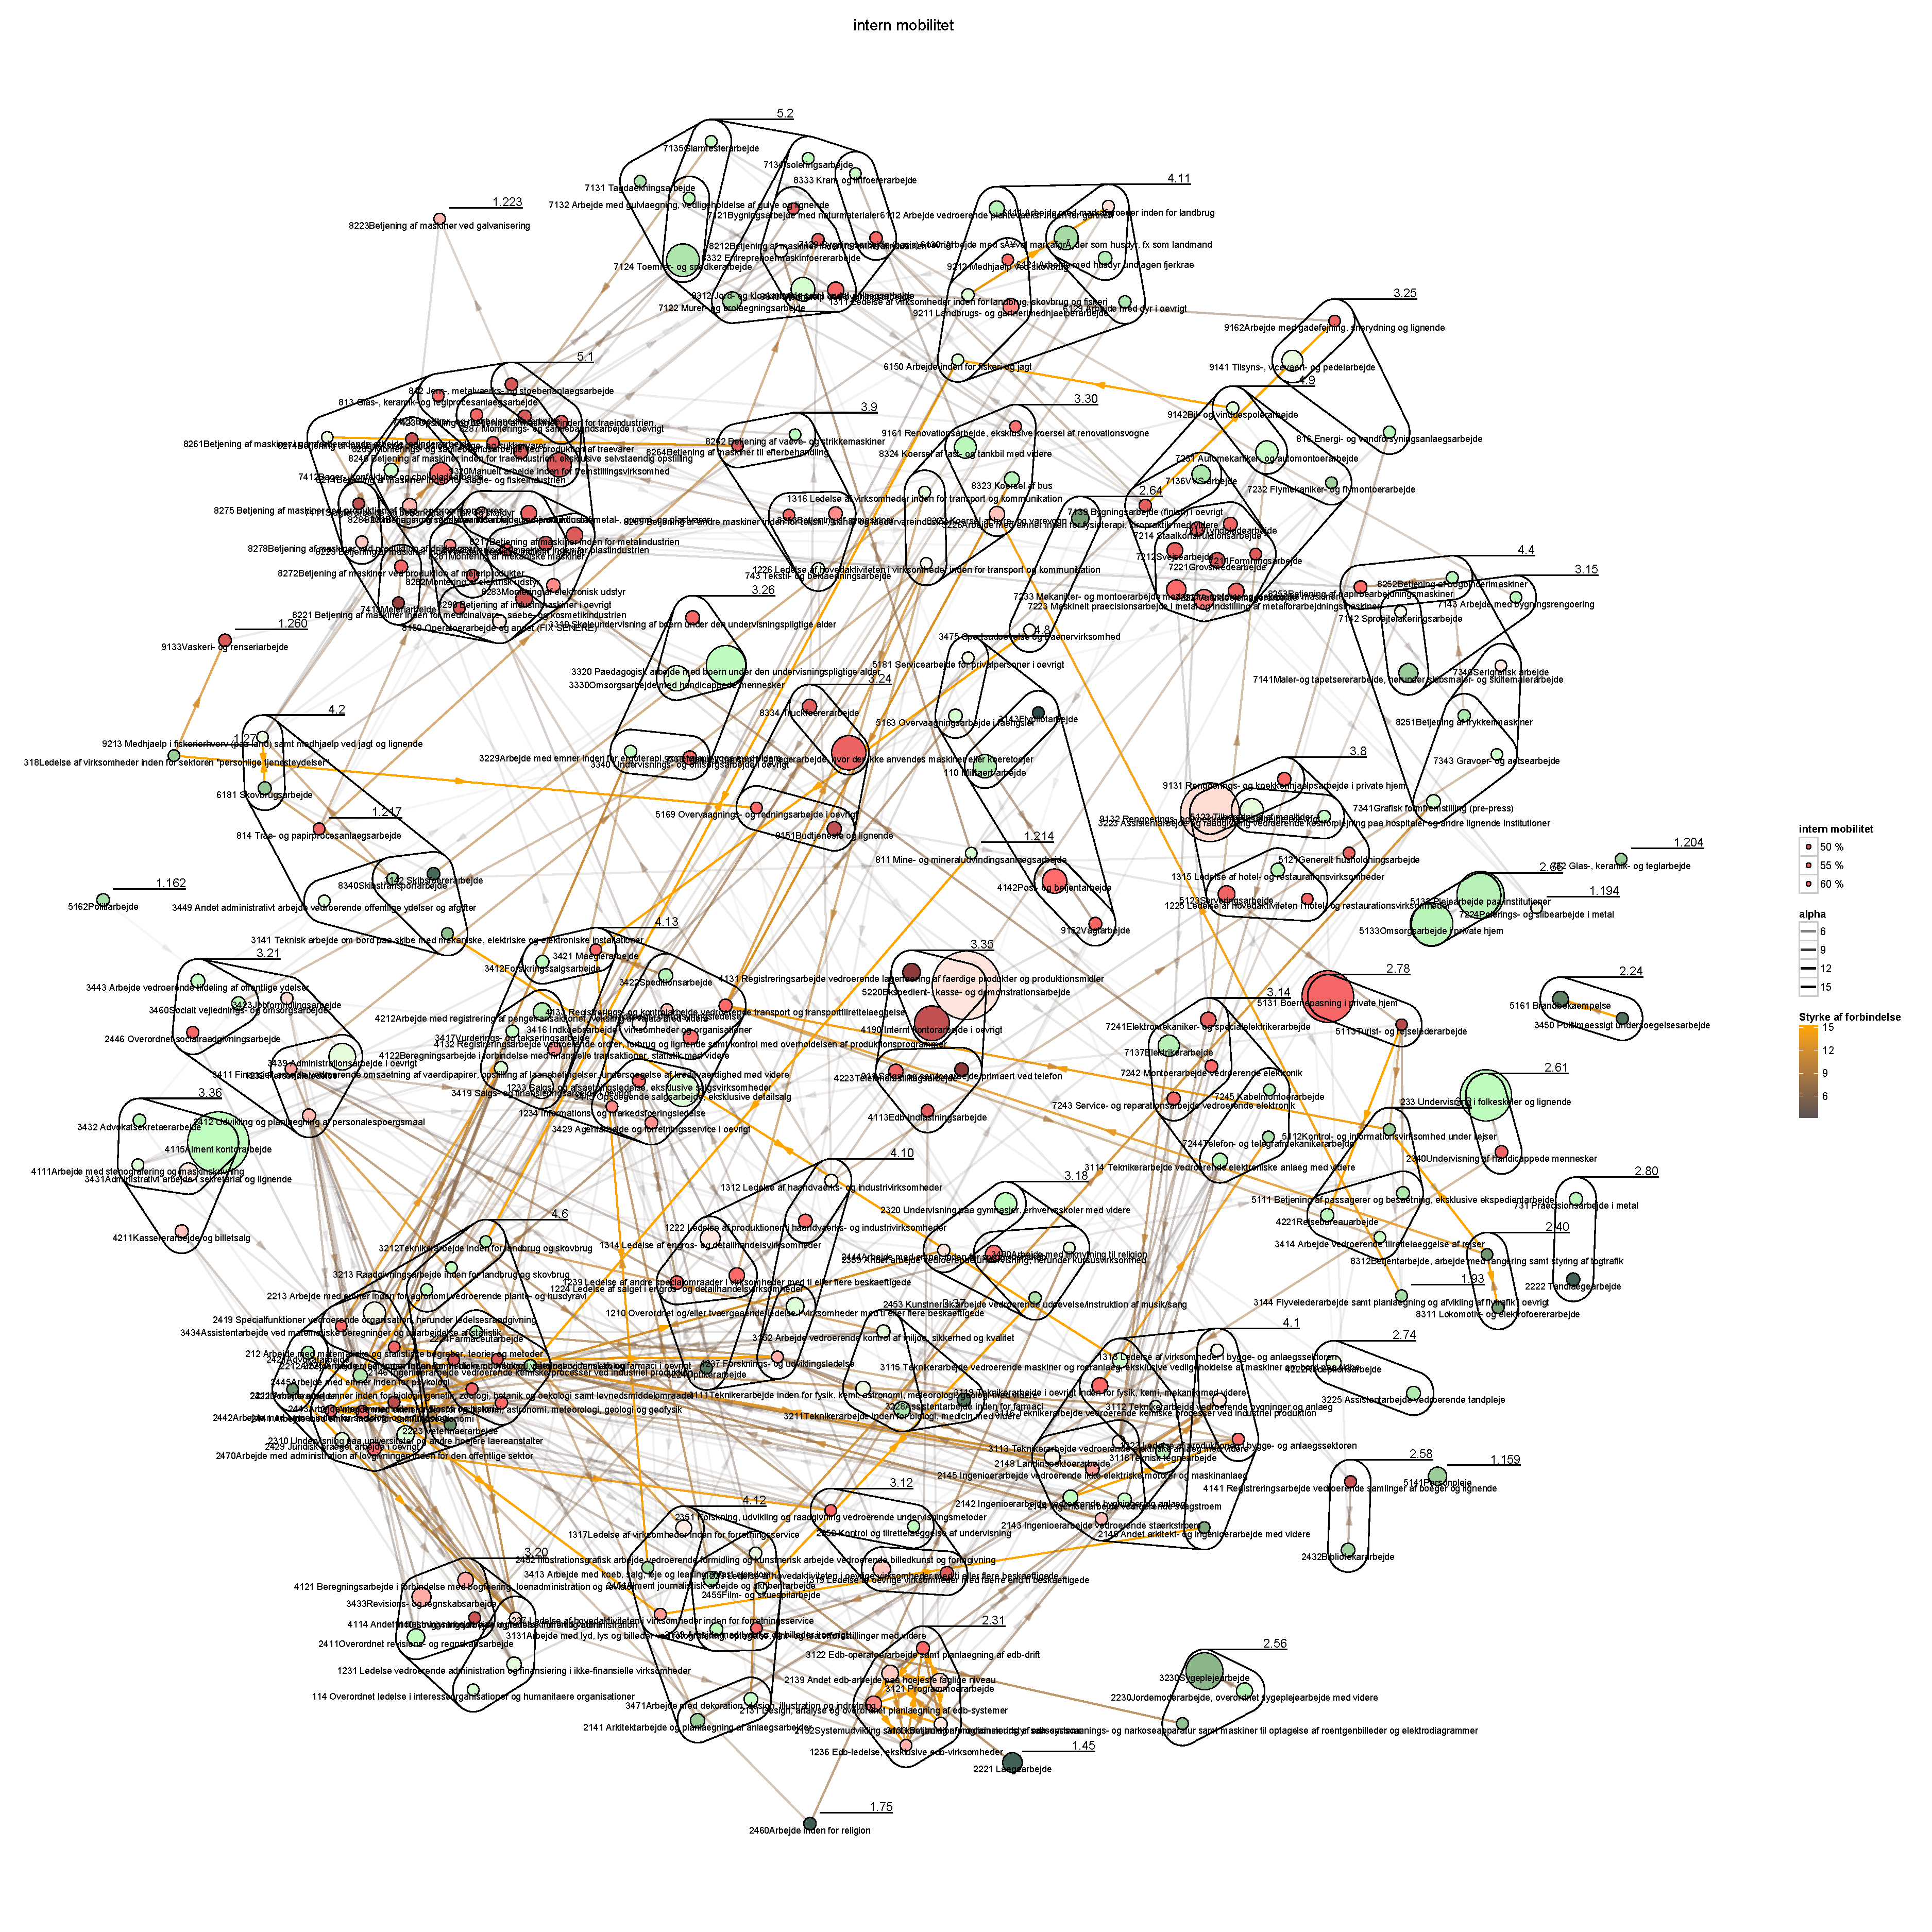
\includegraphics[width=1.0\textwidth]{fig/netvaerkskort/kort_intern_mob.pdf}
\end{center}
\end{figure}
\restoregeometry



\newgeometry{left=-0.01cm,bottom=0.1cm}
\begin{figure}[H]
\begin{center}
	\caption{Netværkskort: Timelønninger}
	\label{appendiks kort timelon}
	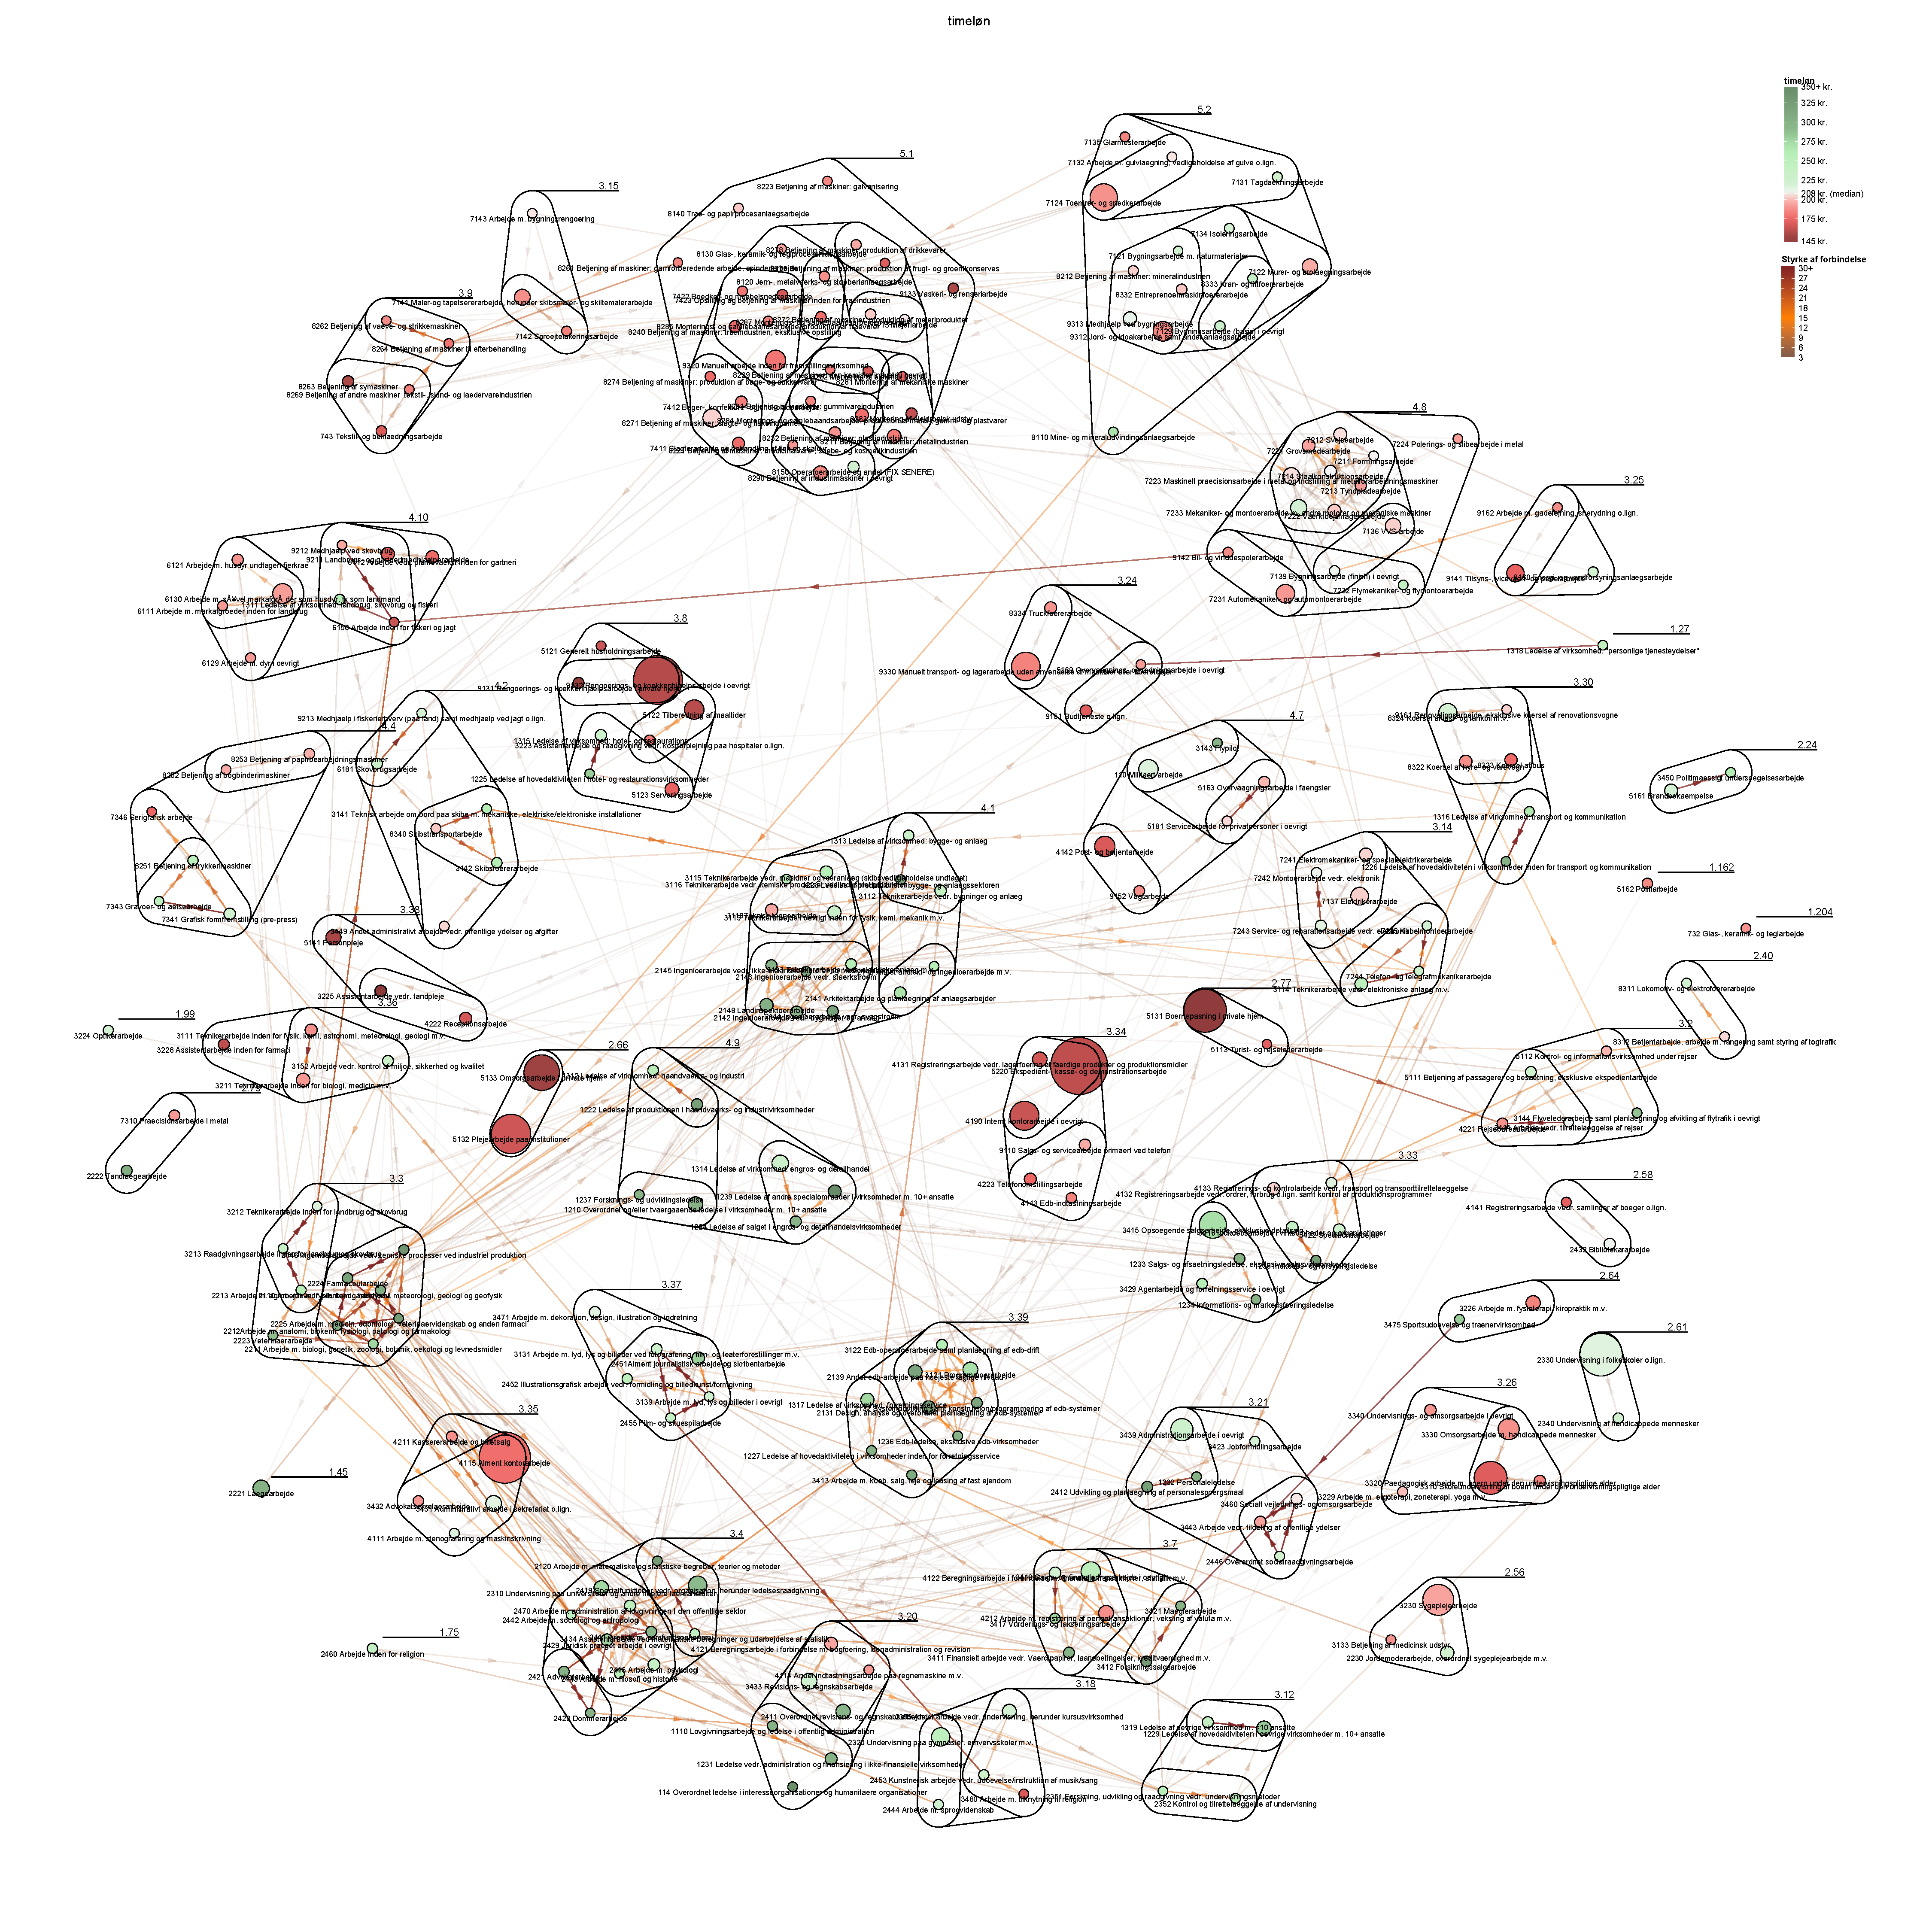
\includegraphics[width=1.0\textwidth]{fig/netvaerkskort/kort_timelon.pdf}
\end{center}
\end{figure}
\restoregeometry



\newgeometry{left=-0.01cm,bottom=0.1cm}
\begin{figure}[H]
\begin{center}
	\caption{Netværkskort: detaljerede forbindelser/edges}
	\label{appendiks kort edges}
	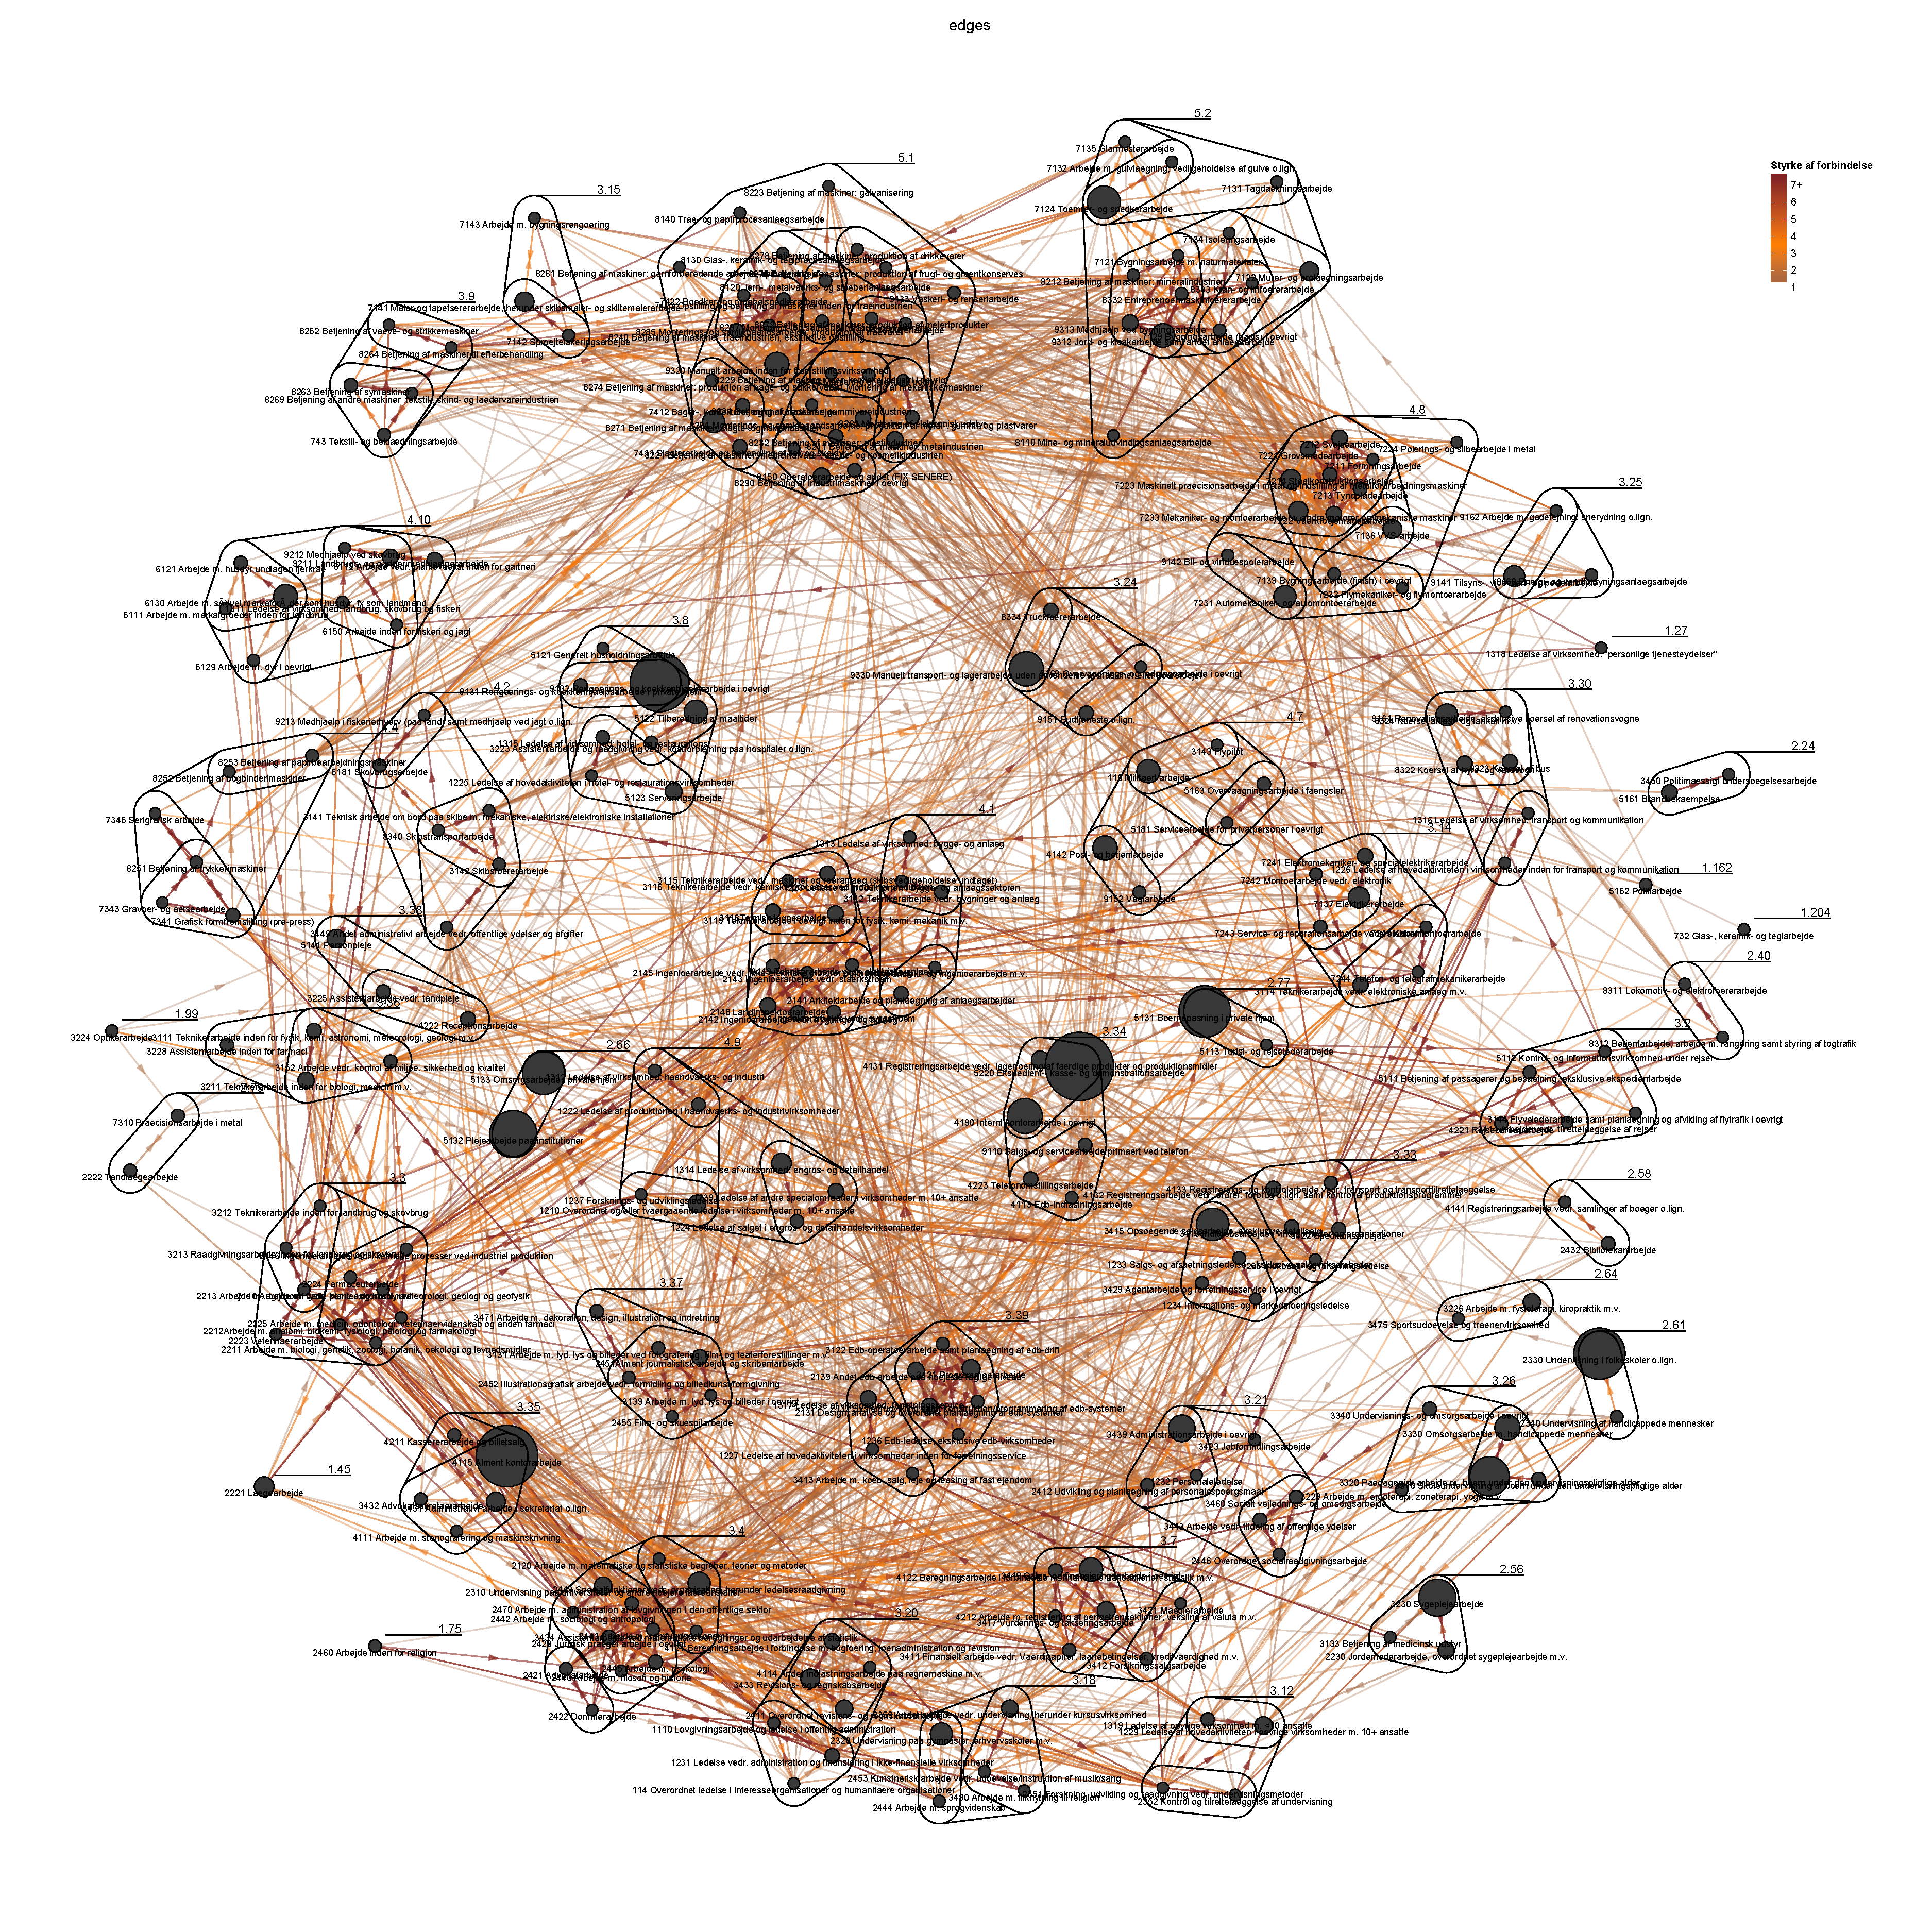
\includegraphics[width=1.0\textwidth]{fig/netvaerkskort/kort_edges.pdf}
\end{center}
\end{figure}
\restoregeometry


% % \input{tex/app_metode_disco}
% % \input{tex/app_metode_baggrundsvariable}

%\end{appendix} 

%\newpage

%%% -------------- Bibliografi ----------------- %%%

\chapter{Litteraturliste \label{litteraturliste}}
%%%%% biblatex definerer alt i preamblet

% \nocite{*} % brug denne for at tage referencer med der ikke citeres i teksten

%%%%% til samlet litteraturliste
% \printbibliography

% %%%%% til opsplittet litteraturliste
\printbibliography[heading=subbibliography,title={Primær litteraturliste},filter=notonline]
\printbibliography[heading=subbibliography,title={Online kilder},type=online]
\printbibliography[heading=subbibliography,title={DST manualer},filter=DST]
\printbibliography[heading=subbibliography,title={Danmarks Statistiks Manualer},type=manual]

\newpage



%%% -------------- slut det hele er slut ----------------- %%%
\end{document}




